\documentclass{format/laszewski} 

\newcommand{\TITLE}{Lecture Notes\\Introduction to Cloud Computing}
\newcommand{\SUBTITLE}{Theory and Practice}
\newcommand{\AUTHOR}{Gregor von Laszewski}
\newcommand{\EMAIL}{laszewski@gmail.com}
\newcommand{\LOCATION}{URL}

\addbibresource{bib/bibliography.bib} % BibTeX bibliography file
\addbibresource{bib/refs-jabref.bib} % BibTeX bibliography file
\defbibheading{bibempty}{}
%%%%%%%%%%%%%%%%%%%%%%%%%%%%%%%%%%%%%%%%%%%%%%%%%%%%%%%%%%%%%%%%%%%%%%
% IMAGE DIRECTORIES
%%%%%%%%%%%%%%%%%%%%%%%%%%%%%%%%%%%%%%%%%%%%%%%%%%%%%%%%%%%%%%%%%%%%%%
\graphicspath{%
{.}%
{images/}%
{section/cloud/chameleon/}%
{section/iot/}%
{section/mapreduce/}%
{section/os/}%
{section/cluster/pi/}%
{section/container/}%
{section/aws/}%
{dest/}%
{dest/section/cloud/chameleon/}%
{dest/section/iot/}%
{dest/section/mapreduce/}%
{dest/section/os/}%
{dest/section/cluster/pi/}%
{dest/section/container/}%
{dest/section/aws/}%
{dest/format/}%
{format/}%
{notebooks/facedetection/}%
{notebooks/}%
{notebooks/opencv/secchi-a/}%
{notebooks/opencv/opencv_files/}%
{notebooks/opencv/secchi/}%
{notebooks/files/}%
{notebooks/facedetection/facedetection_files/}%
{notebooks/scipy/}%
{notebooks/scikit-learn/scikit-learn-k-means_files/}%
{notebooks/fingerprint/}%
{notebooks/opencv/secchi/data/}%
{notebooks/scikit-learn/}%
{notebooks/opencv/}%
}


%https://github.com/cloudmesh/book/blob/master/section/container/kubernetes-fs.md

\begin{document}

\maketitle


\chapterimage{container.png} 
\part{Cloud Container Technologies}

% chktex-file 8
% chktex-file 1

\chapter{Introduction to Containers}
\label{c:container}

\FILENAME

This section covers an introduction to containers that is split up
into four parts. We discuss microservices, serverless computing,
Docker, and kubernetes.

\section{Motivation - Microservices}
\label{s:motivation-microservices}

We discuss the motivation for containers and contrast them to virtual
machines. Additionally we provide a motivation for containers as they
can be used to microservices.

\video{Container}{11:01}{Container A}{https://youtu.be/-HlB0eiwV10}

\section{Motivation - Serverless Computing}
\label{s:motivation-serverless}

We enhance our motivation while contrasting containers and
microservices while relating them to serverless computing. We
anticipate that serverless computing will increase in importance over
the next years

\video{Container}{15:08}{Container B}{https://youtu.be/fxDc5cL6MgQ}

\section{Docker}
\label{s:motivation-docker}

In order for us to use containers, we go beyond the historial
motivation that was introduced in a previous section and focus on
Docker a predominant technology for containers on Windows, Linux, and
OSX

\video{Container}{40:09}{Container C}{https://youtu.be/A2b-LrnoMqg}

\section{Docker and Kubernetes}
\label{s:motivation-docker-kubernetes}

We continue our discussion about docker and introduce kubernetes,
allowing us to run multiple containers on multiple servers building a
cluster of containers.

\video{Container}{50:14}{Container D}{https://youtu.be/V41oi2Bh8Cc}


\section{Resources}

\subsection{Container Orchestration Tools: Compare Kubernetes vs Docker Swarm}

\URL{https://platform9.com/blog/compare-kubernetes-vs-docker-swarm/}

\subsection{Gentle introduction to Containers}

\URL{https://www.slideshare.net/jpetazzo/introduction-docker-linux-containers-lxc}

\subsection{Tutorialspoint}

\URL{https://www.tutorialspoint.com/docker/index.htm}

\URL{https://www.tutorialspoint.com/docker/docker_tutorial.pdf}

\URL{https://www.tutorialspoint.com/docker/docker_pdf_version.htm}



% chktex-file 1
% chktex-file 29

\FILENAME

\section{Intorduction to Docker}
\label{Docker}
\index{Docker}

Docker is the company driving the container movement and the only
container platform provider to address every application across the
hybrid cloud. Today's businesses are under pressure to digitally
transform but are constrained by existing applications and
infrastructure while rationalizing an increasingly diverse portfolio of
clouds, datacenters and application architectures. Docker enables true
independence between applications and infrastructure and developers and
IT ops to unlock their potential and creates a model for better
collaboration and innovation.

\begin{figure}[htbp]
\centering
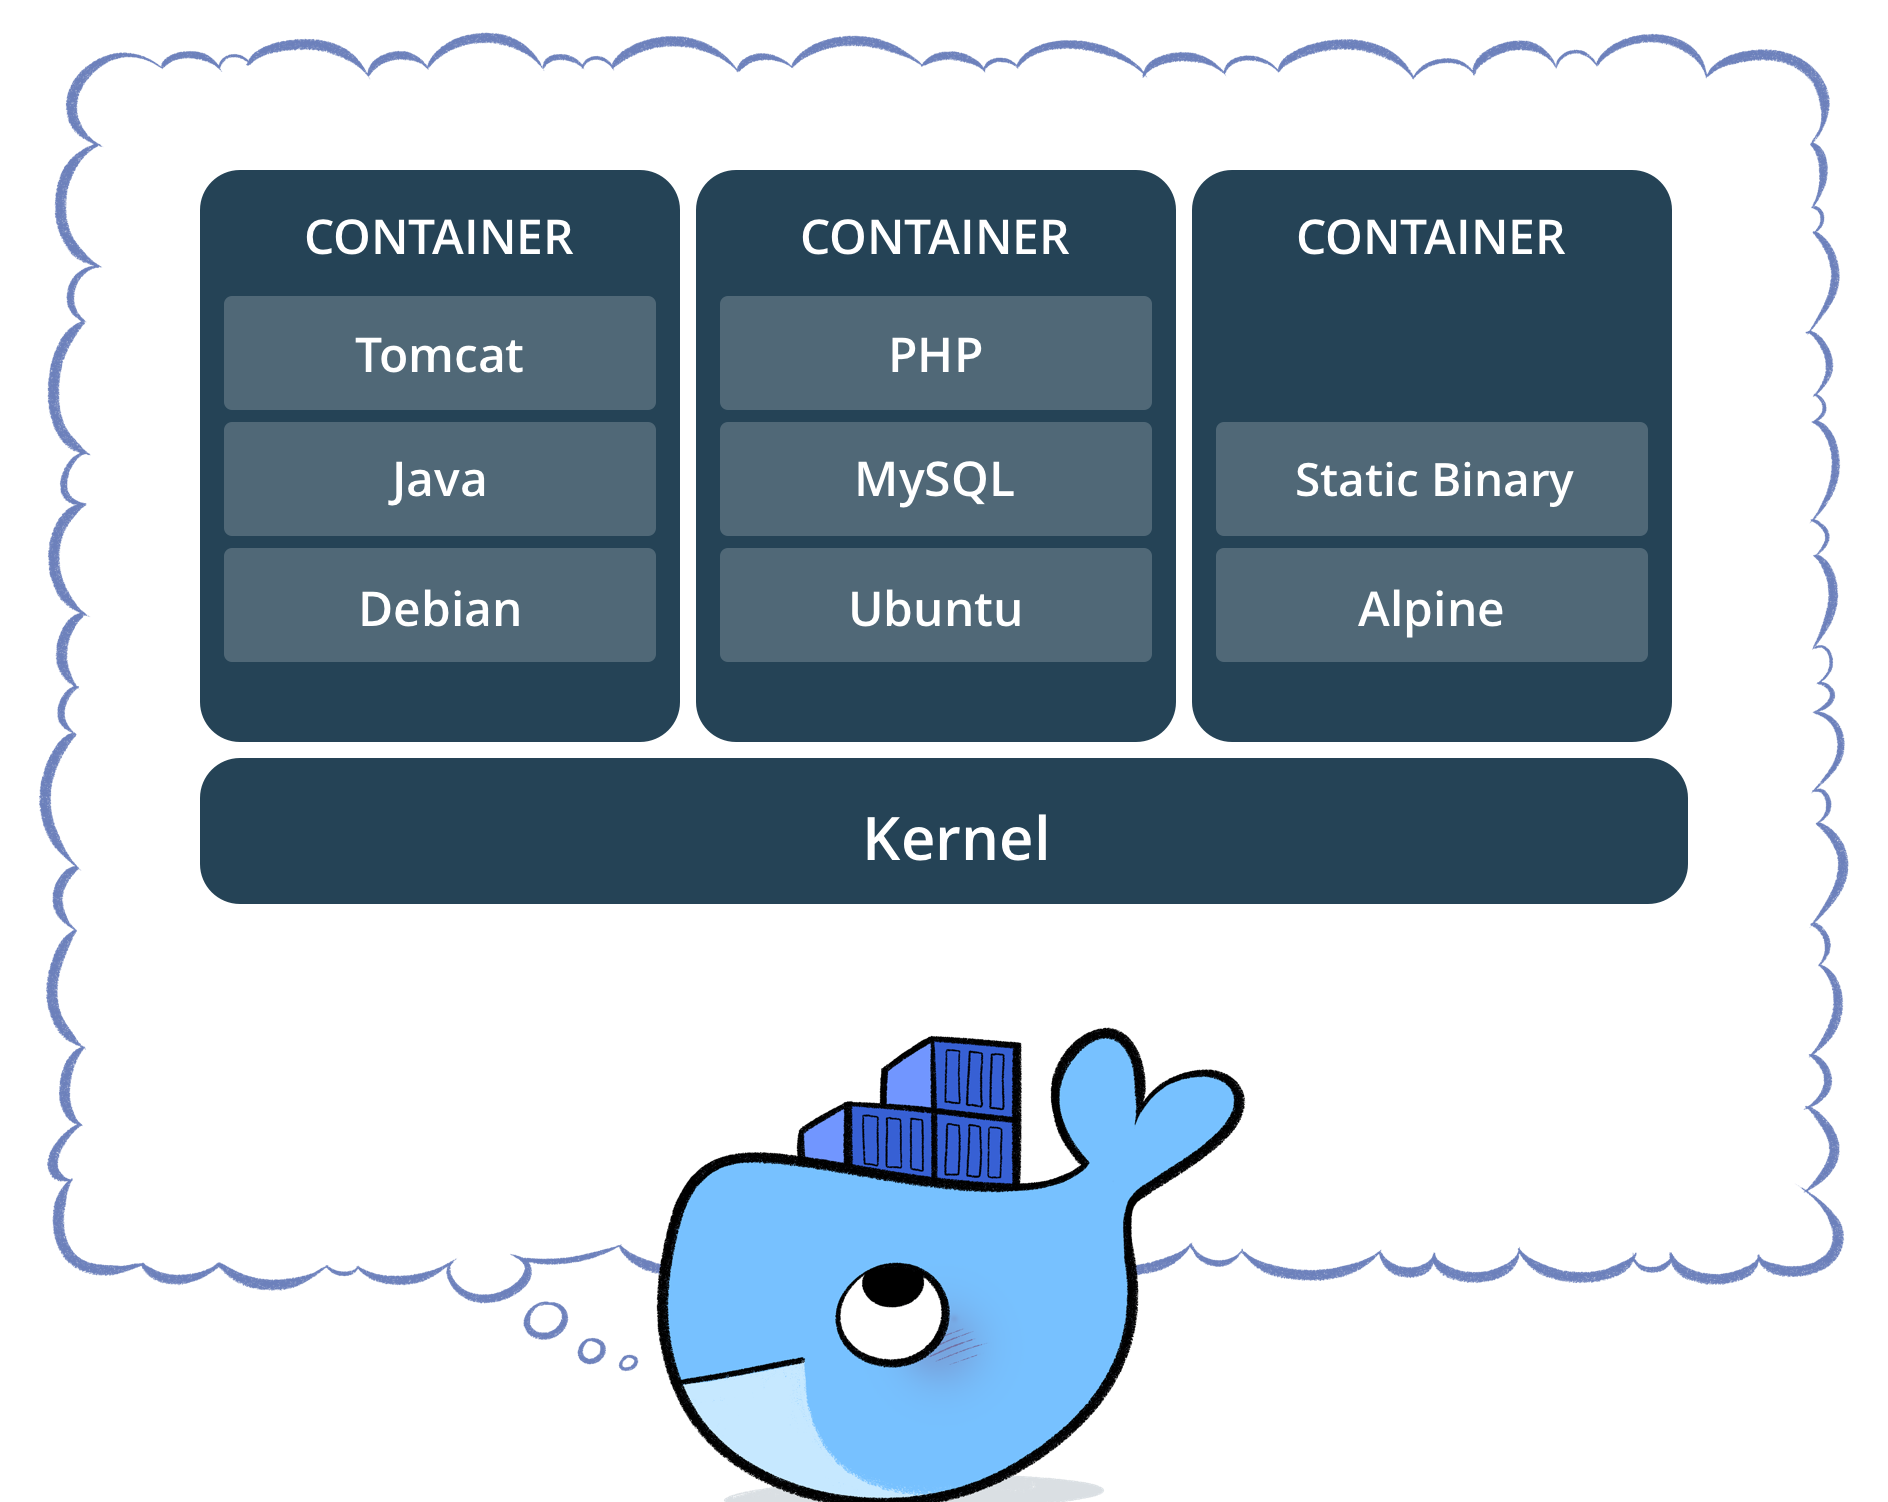
\includegraphics[width=0.7\textwidth]{docker-container.png}
\caption{Docker Containers}
\end{figure}

Image Source
\url{https://www.docker.com/sites/default/files/Package\%20software\%40x2.png}


% chktex-file 1
% chktex-file 13

\chapter{Running Docker Locally}
\label{S:docker-local}
\index{Docker!Local}

\FILENAME\

The official installation documentation for docker can be found by
visiting the following Web page:

\URL{https://www.docker.com/community-edition}

Here you will find a variety of packages, one of which will hopefully
suitable for your operating system. The supported operating systems
currently include:

\begin{itemize}
\item  OSX, Windows, Centos, Debian, Fedora, Ubuntu, AWS, Azure
\end{itemize}

Please chose the one most suitable for you. For your convenience we
provide you with installation instructions for OSX
(Section~\ref{s:docker-osx}), Windows 10 (Section~\ref{s:docker-windows})
and Ubuntu (Section~\ref{s:docker-ubuntu}).

\section{Instillation for OSX}
\label{s:docker-osx}
\index{Docker!Install!OSX}

The docker community edition for OSX can be found at the following link

\URL{https://store.docker.com/editions/community/docker-ce-desktop-mac}

We recommend that at this time you get the version \textit{Docker CE for MAC (stable)}

\URL{https://download.docker.com/mac/stable/Docker.dmg}

Clicking on the link will download a dmg file to your machine, that
you than will need to install by double clicking and allowing access
to the dmg file. Upon installation a \texttt{whale} in the top status
bar shows that Docker is running, and you can access it via a terminal.

\begin{figure}[htb]
\centering

\includegraphics[width=0.5\textwidth]{whale-in-menu-bar.png}
\caption{Docker integrated in the menu bar on OSX}
\end{figure}

\section{Installation for Ubuntu}
\label{s:docker-ubuntu}
\index{Docker!Install!Ubuntu}

In order to instal Docker community edition for Ubuntu, you first have
to register the repository from where you can download it. This can be
achieved as follows:

\begin{lstlisting}[language=bash]
$ sudo apt-get update
$ sudo apt-get install \
    apt-transport-https \
    ca-certificates \
    curl \
    software-properties-common
$ curl -fsSL https://download.docker.com/linux/ubuntu/gpg | sudo apt-key add -
$ sudo apt-key fingerprint 0EBFCD88
$ sudo add-apt-repository \
   "deb [arch=amd64] https://download.docker.com/linux/ubuntu \
   $(lsb_release -cs) \
   stable"
\end{lstlisting}

Now that you have configured the repository location, you can install it
after you have updated the operating system. The update and install is
done as follows:

\begin{lstlisting}[language=bash]
$ sudo apt-get update
$ sudo apt-get install docker-ce
$ sudo apt-get update
\end{lstlisting}
%$


\section{Draft: Installation for Windows 10}
\label{s:docker-windows}
\index{Docker!Install!Windows}

\begin{WARNING}
The instructions for Windows have not passed our quality control. We
look for TAs and student that test out and improve this section.
\end{WARNING}

\TODO{TA: Docker on windows. Please improve and finalize the section}

Before we start we create the following directory:

\begin{lstlisting}[language=bash]
mkdir $HOME/cloudmesh
\end{lstlisting}
%$

We also assume you have installed gitbash and use the a git bash
terminal window for the next steps.

To install Docker on Windows, please download the following files

\URL{https://download.docker.com/win/stable/Docker\%20for\%20Windows\%20Installer.exe}

\URL{https://download.docker.com/win/stable/DockerToolbox.exe}

Move the downloaded files to a directory \verb|$HOME/cloudmesh|

Place the downloaded exe files in the cloudmesh directory we created
earlier. First conduct the Docker installation and then continue with
the Docker Toolbox installation. You can double click the exe files  and
run the installation.

When you are doing the installation, check on the selection in the
installation saying to create shortcuts in your desktop. This way you
can start all the programs from a desktop shortcut.

To run docker, you need to start the \textit{Docker Quickstart
  Terminal} application and it will load all docker and provide a
terminal window in which you can execute docker commands. Once the
terminal is loaded, it will show something like following:

\begin{lstlisting}[language=bash]
$ <username>@<yourpc> ~
\end{lstlisting}
%$



\section{Testing the Install}
\index{Docker!Install!Test}

To test if it works execute the following commands in a terminal:

\begin{lstlisting}[language=bash]
docker version
\end{lstlisting}

You should see an output similar to

\begin{lstlisting}
docker version

Client:
  Version:      17.03.1-ce
  API version:  1.27
  Go version:   go1.7.5
  Git commit:   c6d412e
  Built:        Tue Mar 28 00:40:02 2017
  OS/Arch:      darwin/amd64

Server:
  Version:      17.03.1-ce
  API version:  1.27 (minimum version 1.12)
  Go version:   go1.7.5
  Git commit:   c6d412e
  Built:        Fri Mar 24 00:00:50 2017
  OS/Arch:      linux/amd64
  Experimental: true
\end{lstlisting}

To see if you can run a container use

\begin{lstlisting}[language=bash]
docker run hello-world
\end{lstlisting}

Once executed you should see an output similar to

\begin{lstlisting}[language=bash]
Unable to find image 'hello-world:latest' locally
latest: Pulling from library/hello-world
78445dd45222: Pull complete 
Digest: sha256:c5515758d4c5e1e838e9cd307f6c6a .....
Status: Downloaded newer image for hello-world:latest

Hello from Docker!
This message shows that your installation appears to 
be working correctly.

To generate this message, Docker took the following steps:
1. The Docker client contacted the Docker daemon.
2. The Docker daemon pulled the "hello-world" image 
   from the Docker Hub.
3. The Docker daemon created a new container from that 
   image which runs the executable that produces the 
   output you are currently reading.
4. The Docker daemon streamed that output to the Docker 
   client, which sent it to your terminal.

To try something more ambitious, you can run an Ubuntu container 
with:

$ docker run -it ubuntu bash

Share images, automate workflows, and more with a free Docker ID:
https://cloud.docker.com/

For more examples and ideas, visit:
https://docs.docker.com/engine/userguide/
\end{lstlisting}
%$

\chapter{Running Docker on FutureSystems}\label{S:docker-fg}

\FILENAME

\section{Overview}\label{overview}

This documentation introduces how to run Docker container on
FutureSystems. Currently we have deployed Docker swarm on Echo.

\section{Getting Access}\label{getting-access}

You will need an account on FutureSystems. To verify, try to see if you
can log into india.futuresystems.org. You need to be a member of a valid
FutureSystems project, and had submitted an ssh public key via the
FutureSystems portal.

If your access to the india host has been verified, try to login to the
docker swarm head node with the same username and key:

\begin{quote}
ssh FS_USER@149.165.150.76
\end{quote}

\textbf{NOTE: If you have access to india but not the docker swarm
system, your project may not have been authorized to access the docker
swarm cluster. Send a ticket to FutureSystems ticket system to request
this.}

Once logged in to the docker swarm head node, try to run:

to verify `docker run' works.

\section{Creating a service and deploy to the swarm
cluster}\label{creating-a-service-and-deploy-to-the-swarm-cluster}

While `docker run' can start a container and you may even attach to its
console, the recommended way to use a docker swarm cluster is to create
a service and have it run on the swarm cluster. The service will be
scheduled to one or many number of the nodes of the swarm cluster, based
on the configuration. It's also easy to scale up the service when more
swarm nodes are available. Docker swarm really makes it easier for
service/application developers to focus on the functionality development
but not worrying about how and where to bind the service to some
resources/server. The deployment, access, and scaling up/down when
necessary, are all managed transparently. Thus achieving the new
paradigm of `serverless computing'.

As an example, the following command creates a service and deploy it to
the swarm cluster:

\begin{quote}
docker service create --name notebook\_test -p 9001:8888
jupyter/datascience-notebook start-notebook.sh
--NotebookApp.password=NOTEBOOK\_PASS
\end{quote}

It pulls a published image from docker cloud, starts a container and
runs a script to start the service inside the container with necessary
parameters. The option ``-p 9001:8888'' maps the service port inside the
container (8888) to an external port of the cluster node (9001) so the
service could be accessed from the Internet. In this example, you can
then visit the URL:

\begin{quote}
\url{http://149.165.150.76:9001}
\end{quote}

to access the Jupyter notebook. Using the specified password when you
create the service to login.

Please note the service will be dynamically deployed to a container
instance, which would be allocated to a swarm node based on the
allocation policy. Docker makes this process transparent to the user and
even created mesh routing so you can access the service using the IP
address of the management head node of the swarm cluster, no matter
which actual physical node the service was deployed to.

This also implies that the external port number used has to be free at
the time when the service was created.

Some useful related commands:


\begin{verbatim}
docker service ls
\end{verbatim}

lists the currently running services.

\begin{verbatim}
docker service ps notebook_test
\end{verbatim}

lists the detailed info of the container where the service is running.

\begin{verbatim}
docker node ps NODE
\end{verbatim}

lists all the running containers of a node.

\begin{verbatim}
docker node ls
\end{verbatim}

lists all the nodes in the swarm cluster.

To stop the service and the container:

\begin{verbatim}
docker service rm noteboot_test
\end{verbatim}


\subsection{Create your own service}\label{create-your-own-service}

You can create your own service and run it. To do so, start from a base
image, e.g., a ubuntu image from the docker cloud. Then you could:

\begin{itemize}

\item Run a container from the image and attach to its console to develop
the service, and create a new image from the changed instance using
command `docker commit'.

\item Create a dockerfile, which has the step by step building process of
the service, and then build an image from it.

\end{itemize}

In reality, the first approach is probably useful when you are in the
phase of develop and debug your application/service. Once you have the
step by step instructions developped the latter approach is the
recommended way.

Publish the image to the docker cloud by following this documentation:

\begin{quote}
\url{https://docs.docker.com/docker-cloud/builds/push-images/}
\end{quote}

Please make sure no sensitive information is included in the image to
be published. Alternatively you could publish the image internally to
the swarm cluster.

\paragraph{Publish an image privately within the swarm cluster}
\label{publish-an-image-privately-within-the-swarm-cluster}

\TODO{Fugang: create image for distribution}

Once the image is published and available to the swarm cluster, you
could start a new service from the image similar to the Jupyter Notebook
example.


\chapterimage{rest.png} % Chapter heading image


\section{Dockerized Flask REST API Application}
\label{s:docker-flask-rest} 
\index{Docker!Flask REST API}
\FILENAME

We discuss how to use Docker to deploy a REST service designed using
Python Flask.

\subsection{Prerequisites}

In order to follow our discussion you will need a system on which you
can run docker. THis could either be OSX, LInux, or Windows.

\TODO{Q: WHICH VERSION OF PYTHON?}

\subsubsection{Ubuntu and OSX}

Please use our instructions on installying pyenv.

\subsubsection{Windows}

We start with download Python:

\href{https://www.python.org/ftp/python/2.7.14/python-2.7.14.msi}{Download
Python MSI}

After installing python add an environmental variable by pressing
Windows Key + Pause and Select Advanced system settings. Then add an
environment varible for system variables for the variable PATH which is
already there. And in that add the new variable

\begin{lstlisting}
C:\Python27
\end{lstlisting}

As older python versions do not come or come with an outdated version of
pip, we install it as follows:

\href{https://bootstrap.pypa.io/get-pip.py}{Download Pip Installer
Script}

Now copy this file to

\begin{lstlisting}
C:\Users\<your_username>\cloudmesh\bin
\end{lstlisting}

If you do not have this path please create it, because we will be using
this place to store all the tools we need. Within the bin folder run the
following commands using command line tool or cmd.exe in windows.

\begin{lstlisting}
$ python get-pip.py
\end{lstlisting}
%$

Now add this environmental variable to PATH in System variables the same
way we did earlier by putting the following value

\begin{lstlisting}
C:\Python27\lib\site-packages
C:\Python27\Scripts
\end{lstlisting}

After adding the variables make sure you use a new cmd.exe.

Now continue by installing a Virtualenv installation

\begin{lstlisting}
    $ pip install virtualenv 
\end{lstlisting}
%$

Turn on Hyper-V (Windows Features Turn On and In the list selectHyber V)

Turn on Containers (Windows Features Turn On and In the list select
Hyber V)

Install emacs via chocolatey

\subsection{Activate Virutal Environment}

\subsubsection{Ubuntu and OSX}

\begin{lstlisting}
$ mkdir -p ~/cloudmesh/containers/docker-flask
$ cd ~/cloudmesh/containers/docker-flask
$ virtualenv venv
$ source venv/bin/activate
\end{lstlisting}

\subsubsection{Windows}

Using cmd.exe Please replace with your username.

\begin{lstlisting}
$ mkdir -p C:\Users\<your_username>\cloudmesh\containers\docker-flask
$ cd C:\Users\<your_username>\cloudmesh\containers\docker-flask
$ virtualenv venv
$ venv/Script/activate
\end{lstlisting}

Now you are inside the created virtual environment. The terminal will
look something like

\begin{lstlisting}
(venv)neo$
\end{lstlisting}
%$

\subsection{File Structure}

The File structure takes the following look.

\begin{lstlisting}
docker-flask/[FOLDER]:[BASE PATH : ~/cloudmesh/containers/docker-flask]
    --|Dockerfile [FILE]
    --|requirements.txt [FILE]
    --|app/ [FOLDER]
        --|--|main.py [FILE]
        --|venv [FOLDER]
\end{lstlisting}

\subsubsection{Step 1}

Create requirements.txt file

\paragraph{Ubuntu and OSX}

\begin{lstlisting}
$ emacs requirements.txt
\end{lstlisting}
%$

\paragraph{Windows}

Install an editor such as emacs on Windows. YOu can use chocolatey for
that, or use pycharm. Do not use notepad++

\begin{lstlisting}
emacs requirements.txt
\end{lstlisting}

Include the folllowing content in the requirements.txt file.

\begin{lstlisting}
Flask==0.11.1
\end{lstlisting}

Now run the following command

\begin{lstlisting}
$ pip install -r requirements.txt
\end{lstlisting}
%$

\subsubsection{Step 2}

Then we are going to create thr Dockerfile which includes all the
instructions for the deployment of the REST API on docker.

\paragraph{Ubuntu and OSX}

\begin{lstlisting}
$ emacs Dockerfile
\end{lstlisting}
%$

\paragraph{Windows}

\begin{lstlisting}
emacs Dockerfile
\end{lstlisting}

Include the following content in the Dockerfile

\begin{lstlisting}
FROM tiangolo/uwsgi-nginx-flask:flask
COPY ./app /app
\end{lstlisting}

Here we have created a minimal Dockerfile.

FROM: command tells the image that has to be pulled from the Docker hub.
So in this case for the ease of the task and to keep it simple with
minimum packages we are going to select an image including nginx, flask
and uWSGI.

\begin{enumerate}
\def\labelenumi{\arabic{enumi}.}
\item
  Nginx: An open source software for web serving capability.
\item
  Flask: REST API package in Python
\item
  uWSGI: A server and one of the protocols implemented in WSGI which is
  a protocol used for pure HTTP communications and load balancing.
\end{enumerate}

So this image includes everything we need to work on this tutorial.

COPY: Here it will copy content from app folder created in local machine
to the Docker container.

Now the Dockerfile is completed and we have everything needed to build a
docker image.

\subsubsection{Step 3}

Then we need to creat the main.py file inside the app folder.

\paragraph{Ubuntu and OSX}

\begin{lstlisting}
emacs app/main.py
\end{lstlisting}

\paragraph{Windows}

\begin{lstlisting}
emacs app/main.py
\end{lstlisting}

Then add the following content.

\begin{lstlisting}
from flask import Flask

app = Flask(__name__)

@app.route("/")
def hello():
    return "Hey I am using Docker!"

@app.route("/api/cpu")
def get_cpu():
# ADD CODE TO GET CPU INFO
# USE psutil LIBRARY
    return "SHOW YOUR CPU INFO"

if __name__ == "__main__":
    app.run(host="127.0.0.1", debug=True, port=80)
\end{lstlisting}

After adding the content save and exit emacs.

\subsection{Build Docker Image}

\subsubsection{Ubuntu and OSX}

Now run the following commands.

\begin{lstlisting}
$ cd ~/cloudmesh/containers/docker-flask
$ docker build -t sample-flask-rest-app .
\end{lstlisting}

\subsubsection{Windows}

Run Powershell as administrator and replace with your username.

\begin{lstlisting}
cd C:\Users\<your_username>\cloudmesh\containers\docker-flask
docker build -t sample-flask-rest-app .
\end{lstlisting}

If it builds successfully, you will get the following response

\begin{lstlisting}
$ docker build -t sample-flask-rest-app .
Sending build context to Docker daemon  19.15MB
Step 1/2: FROM tiangolo/uwsgi-nginx-flask:python2.7
 ---> ec43f17def9a
Step 2/2: COPY ./app /app
 ---> e8eb1bff86b8
Successfully built e8eb1bff86b8
Successfully tagged sample-flask-rest-app:latest

Note: Changing any content inside the app folder must be
      updated in the container by rebuilding the image.
\end{lstlisting}
%$

\subsection{Run Docker Image}

Run the following commands to get the REST API hosted on
\url{http://127.0.0.1:80}

\subsubsection{Ubuntu and OSX}

\begin{lstlisting}
$ docker run -p 80:80 -t sample-flask-rest-app
\end{lstlisting}
%$

\subsubsection{Windows}

In Windows powershell Run as adminstrator (use the previous powershell
window)

\begin{lstlisting}
$ docker run -p 80:80 -t sample-flask-rest-app
\end{lstlisting}
%$

Here you may have to grant permission for using this port number. So
please allow that to run.

It will take sometime to load the server once it is loaded and if it
runs successfully you will see a response shown below.

\begin{lstlisting}[basicstyle=\footnotesize]
$ docker run -p 80:80 -t sample-flask-rest-app
Checking for script in /app/prestart.sh
Running script /app/prestart.sh
Running inside /app/prestart.sh, you could add migrations to this file, e.g.:

#! /usr/bin/env bash

# Let the DB start
sleep 10;
# Run migrations
alembic upgrade head

/usr/lib/python2.7/dist-packages/supervisor/options.py:296:
UserWarning: Supervisord is running as root and it is searching
for its configuration file in default locations (including its
current working directory); you probably want to specify a "-c"
argument specifying an absolute path to a configuration file for
improved security.

'Supervisord is running as root and it is searching '
2018-02-19 18:07:46,198 CRIT Supervisor running as root 
           (no user in config file)
2018-02-19 18:07:46,198 WARN Included extra file
           "/etc/supervisor/conf.d/supervisord.conf" during parsing
2018-02-19 18:07:46,204 INFO RPC interface 'supervisor' initialized
2018-02-19 18:07:46,204 CRIT Server 'unix_http_server' 
           running without any
           HTTP authentication checking
2018-02-19 18:07:46,204 INFO supervisord started with pid 7
2018-02-19 18:07:47,207 INFO spawned: 'nginx' with pid 10
2018-02-19 18:07:47,211 INFO spawned: 'uwsgi' with pid 11
[uWSGI] getting INI configuration from /app/uwsgi.ini
[uWSGI] getting INI configuration from /etc/uwsgi/uwsgi.ini
*** Starting uWSGI 2.0.15 (64bit) on [Mon Feb 19 18:07:47 2018] ***
compiled with version: 4.9.2 on 04 February 2018 16:11:35
os: Linux-4.4.0-112-generic #135-Ubuntu SMP 
    Fri Jan 19 11:48:36 UTC 2018
nodename: 7f9706084219
machine: x86_64
clock source: unix
pcre jit disabled
detected number of CPU cores: 8
current working directory: /app
detected binary path: /usr/local/bin/uwsgi
your memory page size is 4096 bytes
detected max file descriptor number: 1048576
lock engine: pthread robust mutexes
thunder lock: disabled (you can enable it with --thunder-lock)
uwsgi socket 0 bound to UNIX address /tmp/uwsgi.sock fd 3
uWSGI running as root, you can use --uid/--gid/--chroot options
*** WARNING: you are running uWSGI as root !!! 
    (use the --uid flag) *** 
Python version: 2.7.14 (default, Dec 12 2017, 16:55:09)  [GCC 4.9.2]
*** Python threads support is disabled. You can enable it 
    with --enable-threads ***
Python main interpreter initialized at 0x1eed1b0
your server socket listen backlog is limited to 100 connections
your mercy for graceful operations on workers is 60 seconds
mapped 1237056 bytes (1208 KB) for 16 cores
*** Operational MODE: preforking ***
WSGI app 0 (mountpoint='') ready in 0 seconds on interpreter 
     0x1eed1b0 pid: 11 (default app)
*** uWSGI is running in multiple interpreter mode ***
spawned uWSGI master process (pid: 11)
spawned uWSGI worker 1 (pid: 14, cores: 1)
spawned uWSGI worker 2 (pid: 15, cores: 1)
2018-02-19 18:07:48,357 INFO success: nginx entered RUNNING 
  state, process has stayed up for > than 1 seconds (startsecs)
2018-02-19 18:07:48,358 INFO success: uwsgi entered RUNNING 
  state, process has stayed up for > than 1 seconds (startsecs)

\end{lstlisting}
%$


Go to this URL: \url{http://127.0.0.1:80}

\paragraph{Additional INFO}


\begin{lstlisting}[basicstyle=\tiny]
$ docker ps -a
CONTAINER ID IMAGE                     COMMAND                  CREATED             STATUS                   PORTS                         NAMES
dc8cccf22216 35ffca69dcc3            "/entrypoint.sh /sta..." 4 minutes ago Up 4 minutes             0.0.0.0:80->80/tcp, 443/tcp   romantic_sammet
e7a45c81b237 sample-flask            "/entrypoint.sh /usr..." 2 days ago    Exited (0) 2 days ago                                  silly_kare
a4b6419016af sample-flask            "/entrypoint.sh /usr..." 2 days ago    Exited (0) 2 days ago                                  musing_lamport
6eb7102a514e prakhar1989/static-site "./wrapper.sh"           5 days ago    Exited (0) 5 days ago                                  competent_borg
f7c6a4710ad2 prakhar1989/static-site "./wrapper.sh"           5 days ago    Exited (0) 5 days ago                                  static-site
361c8812ba90 busybox                 "echo 'hello from bu..." 5 days ago    Exited (0) 5 days ago                                  blissful_wing
350ec9a2609f busybox                 "sh"                     5 days ago    Exited (0) 5 days ago                                  nifty_mahavira
893cb11019f9 hello-world             "/hello"                 5 days ago    Exited (0) 5 days ago                                  competent_spence
1f90a411c746 hello-world             "/hello"                 11 days ago   Exited (0) 11 days ago                                 reverent_raman

$ docker stop dc8cccf22216
dc8cccf22216

$ docker ps -a
CONTAINER ID IMAGE                     COMMAND                  CREATED             STATUS                     PORTS   NAMES
dc8cccf22216 35ffca69dcc3            "/entrypoint.sh /sta..."   4 minutes ago       Exited (137) 5 seconds ago      romantic_sammet
e7a45c81b237 sample-flask            "/entrypoint.sh /usr..."   2 days ago          Exited (0) 2 days ago           silly_kare
a4b6419016af sample-flask            "/entrypoint.sh /usr..."   2 days ago          Exited (0) 2 days ago           musing_lamport
6eb7102a514e prakhar1989/static-site "./wrapper.sh"           5 days ago          Exited (0) 5 days ago             ompetent_borg
f7c6a4710ad2 prakhar1989/static-site "./wrapper.sh"           5 days ago          Exited (0) 5 days ago             tatic-site
361c8812ba90 busybox                 "echo 'hello from bu..."   5 days ago          Exited (0) 5 days ago            blissful_wing
350ec9a2609f busybox                 "sh"                     5 days ago          Exited (0) 5 days ago             ifty_mahavira
893cb11019f9 hello-world             "/hello"                 5 days ago          Exited (0) 5 days ago             ompetent_spence
1f90a411c746 hello-world             "/hello"                 11 days ago         Exited (0) 11 days ago            everent_raman
\end{lstlisting}


\paragraph{Deleting Docker Conatiner first and then remove Docker Image}


\begin{lstlisting}[basicstyle=\tiny]
$ docker images
REPOSITORY                   TAG                 IMAGE ID            CREATED             SIZE
sample-flask-rest-app        latest              8b3246425402        8 minutes ago       697MB
<none>                       <none>              35ffca69dcc3        10 minutes ago      697MB
sample-flask                 latest              b763c65ae11b        2 days ago          709MB
my-awesome-nginx             v3                  56cb2d15e863        3 days ago          16.8MB
tiangolo/uwsgi-nginx-flask   flask               3ab637f17463        2 weeks ago         709MB
tiangolo/uwsgi-nginx-flask   python2.7           ec43f17def9a        2 weeks ago         697MB
ubuntu                       16.04               0458a4468cbc        3 weeks ago         112MB
ubuntu                       latest              0458a4468cbc        3 weeks ago         112MB
busybox                      latest              5b0d59026729        3 weeks ago         1.15MB
nginx                        alpine              bb00c21b4edf        5 weeks ago         16.8MB
hello-world                  latest              f2a91732366c        3 months ago        1.85kB
prakhar1989/static-site      latest              f01030e1dcf3        2 years ago         134MB


$ docker ps -a
CONTAINER ID IMAGE                     COMMAND                  CREATED             STATUS                   PORTS NAMES
74b9b994c9bd sample-flask-rest-app   "/entrypoint.sh /sta..." 2 minutes ago  Exited (137) About a minute ago       infallible_mahavira
dc8cccf22216 35ffca69dcc3            "/entrypoint.sh /sta..." 10 minutes ago Exited (137) 5 minutes ago            romantic_sammet
e7a45c81b237 sample-flask            "/entrypoint.sh /usr..." 2 days ago     Exited (0) 2 days ago                 silly_kare
a4b6419016af sample-flask            "/entrypoint.sh /usr..." 2 days ago     Exited (0) 2 days ago                 musing_lamport
6eb7102a514e prakhar1989/static-site "./wrapper.sh"           5 days ago     Exited (0) 5 days ago                 competent_borg
f7c6a4710ad2 prakhar1989/static-site "./wrapper.sh"           5 days ago     Exited (0) 5 days ago                 static-site
361c8812ba90 busybox                 "echo 'hello from bu..." 5 days ago     Exited (0) 5 days ago                 blissful_wing
350ec9a2609f busybox                 "sh"                     5 days ago     Exited (0) 5 days ago                 nifty_mahavira
893cb11019f9 hello-world             "/hello"                 5 days ago     Exited (0) 5 days ago                 competent_spence
1f90a411c746 hello-world             "/hello"                 11 days ago    Exited (0) 11 days ago                reverent_raman


$ docker rm 74b9b994c9bd
74b9b994c9bd


$ docker ps -a
CONTAINER ID IMAGE                     COMMAND                  CREATED             STATUS              PORTS NAMES
dc8cccf22216 35ffca69dcc3            "/entrypoint.sh /sta..." 10 minutes ago Exited (137) 5 minutes ago       romantic_sammet
e7a45c81b237 sample-flask            "/entrypoint.sh /usr..." 2 days ago     Exited (0) 2 days ago            silly_kare
a4b6419016af sample-flask            "/entrypoint.sh /usr..." 2 days ago     Exited (0) 2 days ago            musing_lamport
6eb7102a514e prakhar1989/static-site "./wrapper.sh"           5 days ago     Exited (0) 5 days ago            competent_borg
f7c6a4710ad2 prakhar1989/static-site "./wrapper.sh"           5 days ago     Exited (0) 5 days ago            static-site
361c8812ba90 busybox                 "echo 'hello from bu..." 5 days ago     Exited (0) 5 days ago            blissful_wing
350ec9a2609f busybox                 "sh"                     5 days ago     Exited (0) 5 days ago            nifty_mahavira
893cb11019f9 hello-world             "/hello"                 5 days ago     Exited (0) 5 days ago            competent_spence
1f90a411c746 hello-world             "/hello"                 11 days ago    Exited (0) 11 days ago           reverent_raman


$ docker images
REPOSITORY                 TAG       IMAGE ID     CREATED        SIZE
sample-flask-rest-app      latest    8b3246425402 8 minutes ago  697MB
<none>                     <none>    35ffca69dcc3 10 minutes ago 697MB
sample-flask               latest    b763c65ae11b 2 days ago     709MB
my-awesome-nginx           v3        56cb2d15e863 2 days ago     16.8MB
tiangolo/uwsgi-nginx-flask flask     3ab637f17463 2 weeks ago    709MB
tiangolo/uwsgi-nginx-flask python2.7 ec43f17def9a 2 weeks ago    697MB
ubuntu                     16.04     0458a4468cbc 3 weeks ago    112MB
ubuntu                     latest    0458a4468cbc 3 weeks ago    112MB
busybox                    latest    5b0d59026729 3 weeks ago    1.15MB
nginx                      alpine    bb00c21b4edf 5 weeks ago    16.8MB
hello-world                latest    f2a91732366c 3 months ago   1.85kB
prakhar1989/static-site    latest    f01030e1dcf3 2 years ago    134MB


$ docker rmi 8b3246425402
Untagged: sample-flask-rest-app:latest
Deleted: sha256:8b3246425402b55aa5c4cf02cc5ad9ebd880b9fef639529b81495e778e3b3246
Deleted: sha256:639497d8f8bfa7cf497dfc142c8cc9d9b0b6b8689c777b9daa185c618b33d03c
\end{lstlisting}

%$


\chapterimage{container.png} % Chapter heading image
% chktex-file 1
% chktex-file 29

\FILENAME

\chapter{Introduction to Kubernetes}
\index{Kubernetes}

\section{Topics Covered and Learning Outcome}

\begin{itemize}
\item What is Kubernetes?
\item What are containers?
\item Cluster components in Kubernetes
\item Basic Units in Kubernetes
\item Run an example with Minikube
\item Interactive online tutorial
\item Have a solid understanding of Containers and Kubernetes
\item Understand the CLuster components of Kubernetes
\item Understand the terminology of Kubernetes
\item Gain practical experience with kubernetes
\item With minikube
\item With an interactive online tutorial
\end{itemize}

\section{What is Kubernetes?}

Kubernetes is an open-source platform designed to automate deploying,
scaling, and operating application containers.
\url{https://kubernetes.io/docs/concepts/overview/what-is-kubernetes/}

With Kubernetes, you can:

\begin{itemize}

\item Deploy your applications quickly and predictably.
\item Scale your applications on the fly.
\item Roll out new features seamlessly.
\item Limit hardware usage to required resources only.
\item Run applications in public and private clouds.
\end{itemize}

Kubernetes is

\begin{itemize}

\item Portable: public, private, hybrid, multi-cloud
\item Extensible: modular, pluggable, hookable, composable
\item Self-healing: auto-placement, auto-restart, auto-replication,
  auto-scaling
\end{itemize}

\section{What are containers?}

\begin{figure}[htbp]
\centering
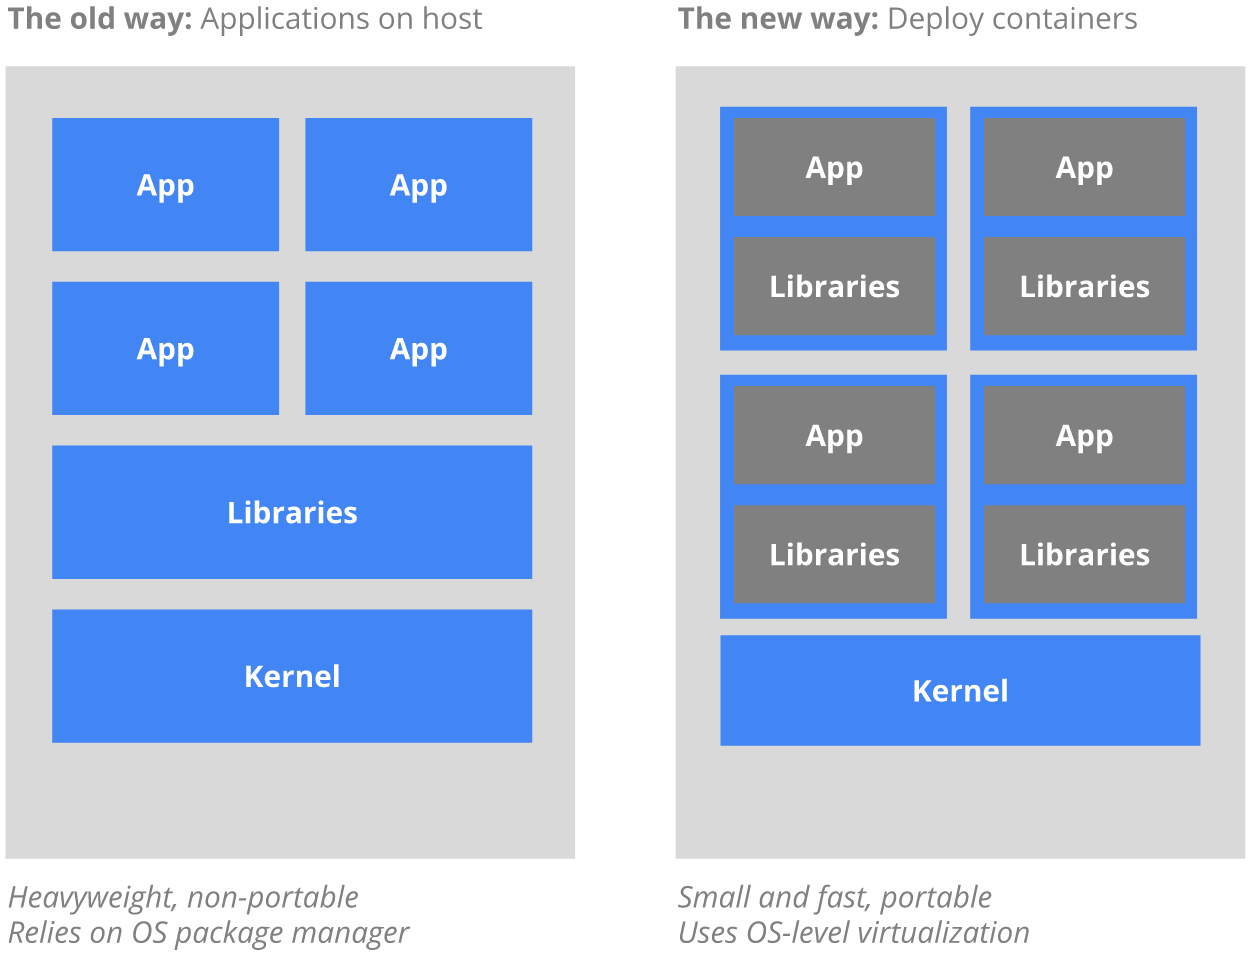
\includegraphics[width=0.8\textwidth]{why_containers.png}
\caption{Kubernetes Containers}
\end{figure}

Image source:

\URL{https://d33wubrfki0l68.cloudfront.net/e7b766e0175f30ae37f7e0e349b87cfe2034a1ae/3e391/images/docs/why_containers.svg}

\section{Terminology}

\begin{description}

\item[Pods:]\index{Pods} A pod (as in a pod of whales or pea pod) is a
  group of one or more containers (such as Docker containers), with
  shared storage/network, and a specification for how to run the
  containers. A pod's contents are always co-located and co-scheduled,
  and run in a shared context. A pod models an application-specific
  \textit{logical host}. It contains one or more application
  containers which are relatively tightly coupled. In a pre-container
  world, they would have executed on the same physical or virtual
  machine.

\item[Services:]\index{Kuberneted!Services} Service is an abstraction
  which defines a logical set of Pods and a policy by which to access
  them. Sometimes they are called a micro-service. The set of Pods
  targeted by a Service is (usually) determined by a Label Selector.

\item[Deployments:]\index{Kuberneted!Deplyments} A Deployment
  controller provides declarative updates for Pods and
  ReplicaSets. You describe a desired state in a Deployment object,
  and the Deployment controller changes the actual state to the
  desired state at a controlled rate. You can define Deployments to
  create new ReplicaSets, or to remove existing Deployments and adopt
  all their resources with new Deployments.

\end{description}

\section{Kubernetes Architecture}

\FIGURE{htb} 
    {1.0}
    {images/kubernetes.png}
    {Kubernetes (Source: Google)}
    {F:tas-arch} 

\section{Minikube}
\index{Kubernetes!Minikube}

\begin{enumerate}
\item minikube installation
\item minikube hello-minikube
\end{enumerate}

\subsection{Install minikube}

\paragraph{OSX}\label{osx}

\begin{lstlisting}[language=bash]
curl -Lo minikube https://storage.googleapis.com/minikube/releases/v0.25.0/minikube-darwin-amd64 && chmod +x minikube && sudo mv minikube /usr/local/bin/
\end{lstlisting}

\paragraph{Windows 10}\label{windows-10}

We assume that you have installed Oracle VirtualBox in your machine
which must be a version 5.x.x.

Initially, we need to download two executables.

\href{http://storage.googleapis.com/kubernetes-release/release/v1.4.0/bin/windows/amd64/kubectl.exe}{Download
Kubectl}

\href{https://storage.googleapis.com/minikube/releases/v0.25.0/minikube-windows-amd64.exe}{Download
Minikube}

After downloading these two executables place them in the cloudmesh
directory we earlier created. Rename the \verb|minikube-windows-amd64.exe|
to \verb|minikube.exe|. Makesure minikube.exe and kubectl.exe lie in the
same directory.

\paragraph{Linux}\label{linux}

\begin{lstlisting}[language=bash]
curl -Lo minikube https://storage.googleapis.com/minikube/releases/v0.25.0/minikube-linux-amd64 && chmod +x minikube && sudo mv minikube /usr/local/bin/
\end{lstlisting}

Installing KVM2 is important for Ubuntu distributions

\begin{lstlisting}[language=bash]
$ sudo apt install libvirt-bin qemu-kvm
$ sudo usermod -a -G libvirtd $(whoami)
$ newgrp libvirtd
\end{lstlisting}

We are going to run minikube using KVM2 libraries instead of virtualbox
libraries for windows installation.

Then install the drivers for KVM2,

\begin{lstlisting}[language=bash]
$ curl -LO https://storage.googleapis.com/minikube/releases/latest/docker-machine-driver-kvm2 && chmod +x docker-machine-driver-kvm2 && sudo mv docker-machine-driver-kvm2 /usr/bin/
\end{lstlisting}
%$

\subsection{Start a cluster using Minikube}

\paragraph{OSX Minikube Start}

\begin{lstlisting}[language=bash]
$ minikube start
\end{lstlisting}
%$

\paragraph{Ubuntu Minikube Start}

\begin{lstlisting}[language=bash]
minikube start --vm-driver=kvm2
\end{lstlisting}

\paragraph{Windows 10 Minikube Start}

In this case you must run Windows PowerShell as administrator. For
this search for the application in search and right click and click Run
as administrator. If you are an administrator it will run automatically
but if you are not please make sure you provide the admin login
information in the pop up.

\begin{lstlisting}[language=bash]
$ cd  C:\Users\<username>\Documents\cloudmesh
$ .\minikube.exe start --vm-driver="virtualbox"
\end{lstlisting}

\subsection{Create a deployment}

\begin{lstlisting}[language=bash]
$ kubectl run hello-minikube --image=k8s.gcr.io/echoserver:1.4 --port=8080
\end{lstlisting}

\subsection{Expose the service}

\begin{lstlisting}[language=bash]
$ kubectl expose deployment hello-minikube --type=NodePort
\end{lstlisting}

\subsection{Check running status}

This step is to make sure you have a pod up and running.

\begin{lstlisting}[language=bash]
$ kubectl get pod
\end{lstlisting}

\subsection{Call service api}

\begin{lstlisting}[language=bash]
$ curl $(minikube service hello-minikube --url)
\end{lstlisting}

\subsection{Take a look from Dashboard}

\begin{lstlisting}[language=bash]
$ minikube dashboard
\end{lstlisting}

If you want to get an interactive dashboard,

\begin{lstlisting}[language=bash]
$ .\minikube.exe dashboard --url=true
http://192.168.99.101:30000
\end{lstlisting}

Browse to http://192.168.99.101:30000 in your web browser and it will
provide a GUI dashboard regarding minikube.

\subsection{Delete the service and deployment}

\begin{lstlisting}[language=bash]
$ kubectl delete service hello-minikube
$ kubectl delete deployment hello-minikube
\end{lstlisting}

\subsection{Stop the cluster}

For all platforms we can use the following command.

\begin{lstlisting}[language=bash]
$ minikube stop
\end{lstlisting}

\section{Interactive Tutorial Online}

\begin{itemize}

\item
  Start cluster
  https://kubernetes.io/docs/tutorials/kubernetes-basics/cluster-interactive/
\item
  Deploy app
  https://kubernetes.io/docs/tutorials/kubernetes-basics/cluster-interactive
\item
  Explore
  https://kubernetes.io/docs/tutorials/kubernetes-basics/explore-intro/
\item
  Expose
  https://kubernetes.io/docs/tutorials/kubernetes-basics/expose-intro/
\item
  Scale
  https://kubernetes.io/docs/tutorials/kubernetes-basics/scale-intro/
\item
  Update
  https://kubernetes.io/docs/tutorials/kubernetes-basics/update-interactive/
\item
  MiniKube
  https://kubernetes.io/docs/tutorials/stateless-application/hello-minikube/
\end{itemize}

\MDNAME\
%%%%%%%%%%%%%%%%%%%%%%%%%%%%%%%%%%%%%%%%%%%%%%%%%%%%%%%%%%%%%%%%%%%%%%%%%%%%%%%
% DO NOT MODIFY THIS FILE
%%%%%%%%%%%%%%%%%%%%%%%%%%%%%%%%%%%%%%%%%%%%%%%%%%%%%%%%%%%%%%%%%%%%%%%%%%%%%%%

\section{Using Kubernetes on FutureSystems}

\label{s:kubernetes-fs}

\index{Kubernetes!Futuresystems} \index{Futuresystems!Kubernetes}

This section introduces you on how to use the Kubernetes cluster on
FutureSystems. Currently we have deployed kubernetes on our cluster
called \emph{echo}.

\subsection{Getting Access}

You will need an account on FutureSystems and upload the ssh key to the
FutureSystems portal from the computer from which you want to login to
echo. To verify, if you have access try to see if you can log into
india.futuresystems.org. You need to be a member of a valid
FutureSystems project.

If you have verified that you haveaccess to the india, you can now try
to login to the kubernetes cluster head node with the same username and
key:

At this time we ask you to use the following IP address to communicate
with echo via its head node:

\begin{lstlisting}
149.165.150.85
\end{lstlisting}

To login to echo use the command

\begin{lstlisting}
ssh FS_USERNAME@149.165.150.85
\end{lstlisting}

where FS\_USERUSER is the username you have on futureSystems.

\textbf{NOTE: If you have access to india but not the kubernetes
software, your project may not have been authorized to access the
kubernetes cluster. Send a ticket to FutureSystems ticket system to
request this.}

Once you are logged in to the kubernetes cluster head node, try to run:

\begin{lstlisting}
kubectl get pods
\end{lstlisting}

This will let you know if you have access to kubernetes and verifies if
the kubectl command works for you. Naturally it will also list the pods.

\subsection{Example Use}

The following command runs an image called nginx with two replicas:

\begin{lstlisting}
kubectl run nginx --replicas=2 --image=nginx --port=80
\end{lstlisting}

As a result of this one deployment was created, and two PODs are created
and started. To see the deployment, please use the command

\begin{lstlisting}
kubectl get deployment
\end{lstlisting}

This will result in the following output

\begin{lstlisting}
NAME      DESIRED   CURRENT   UP-TO-DATE   AVAILABLE   AGE
nginx     2         2         2            2           7m
\end{lstlisting}

To see the pods please use the command

\begin{lstlisting}
kubectl get pods
\end{lstlisting}

This will result in the following output

\begin{lstlisting}
NAME                   READY STATUS  RESTARTS AGE
nginx-7587c6fdb6-4jnh6 1/1   Running 0        7m
nginx-7587c6fdb6-pxpsz 1/1   Running 0        7m
\end{lstlisting}

If we want to see more detailed information we cn use the command

\begin{lstlisting}
kubectl get pods -o wide
\end{lstlisting}

\begin{lstlisting}
NAME                   READY STATUS  RESTARTS AGE IP        NODE
nginx-75...-4jnh6 1/1   Running 0        8m  192.168.56.2   e003
nginx-75...-pxpsz 1/1   Running 0        8m  192.168.255.66 e005
\end{lstlisting}

Please note the IP address field. Now if we try to access the nginx
homepage with wget (or curl)

\begin{lstlisting}
wget 192.168.56.2
\end{lstlisting}

we see the following output:

\begin{lstlisting}
--2018-02-20 14:05:59--  http://192.168.56.2/
Connecting to 192.168.56.2:80... connected.
HTTP request sent, awaiting response... 200 OK
Length: 612 [text/html]
Saving to: 'index.html'

index.html    100%[=========>]     612  --.-KB/s    in 0s

2018-02-20 14:05:59 (38.9 MB/s) - 'index.html' saved [612/612]
\end{lstlisting}

It verifies that the specified image was running, and it is accessible
from within the cluster.

Next we need to start thinking about how we access this web server from
outside the cluster. We can explicitly exposing the service with the
following command

\begin{lstlisting}
kubectl expose deployment nginx --type=NodePort --name=999-nginx-ext
\end{lstlisting}

We will see the response

\begin{lstlisting}
service "nginx-external" exposed
\end{lstlisting}

To find the exposed ip adresses, we simply issue the command

\begin{lstlisting}
kubectl get svc
\end{lstlisting}

We se somthing like this

\begin{lstlisting}
NAME          TYPE      CLUSTER-IP    EXTERN PORT(S)      AGE
                                      AL-IP
kubernetes    ClusterIP 10.96.0.1     <none> 443/TCP      8h
999-nginx-ext NodePort  10.96.183.189 <none> 80:30275/TCP 6s
\end{lstlisting}

please note that we have given a unique name.

\begin{IU}

You could use your username or if you use one of our classes your
hid. The number part will typically be suficient.  For class users
that do not use the hid in the name we will terminate all instances
without notification. In addition, we like you explicitly to add
"-ext" to every container that is exposed to the internet. Naturally
we want you to shut down such services if they are not in use. Failure
to do so may result in termination of the service without notice, and
in the worst case revocation of your priveledges to use *echo*.

\end{IU}

In our example you will find the port on which our service is exposed
and remaped to. We find the port \textbf{30275} in the value
\textbf{80:30275/TCP} in the ports column for the running container.

Now if we visit this URL, which is the public IP of the head node
followed by the exposed port number

\begin{lstlisting}
http://149.165.150.85:30275
\end{lstlisting}

you should see the `Welcome to nginx' page.

\subsection{Exercises}

\begin{exercise}
Explore more complex service examples.
\end{exercise}

\begin{exercise}
Explore constructing a complex web app with multiple services.
\end{exercise}

\begin{exercise}
Define a deployment with a yaml file declaratively.
\end{exercise}



% chktex-file 1
% chktex-file 36
% chktex-file 25
% chktex-file 13
% chktex-file 8
% chktex-file 26

\FILENAME

\chapter{Apache Hadoop using Docker}


In this section we will explore the 
Map/Reduce framework using Hadoop provided through a Docker
container. The example that we use in this session is similar to
WordCount but simple calculations are added e.g.\ minimum, maximum,
average and standard deviation values using several input files which
contain float numbers.

\section{Draft: Creating the Hadoop Container}

\section{Hadoop from Docker}

Build a docker image by Dockerfile from:

\begin{lstlisting}
mkdir hadoop
cd hadoop
wget https://raw.githubusercontent.com/cloudmesh/book/master/examples/docker/hadoop/Dockerfile
docker build -t cloudmesh/hadoop .
\end{lstlisting}

%We use a Docker image from Docker Hub:
%(\url{https://hub.docker.com/r/lee212/e222/}) The base image is from
%sequenceiq/hadoop and the example with input data is added for this
%tutorial.

\section{Start a Hadoop container}

\begin{lstlisting}
docker run -it cloudmesh/hadoop /etc/bootstrap.sh -bash
%docker run -it lee212/e222 /etc/bootstrap.sh -bash
\end{lstlisting}

It may take a few minutes at first to download image layers which are
about 847MB\@.

\section{Statistical Example with Hadoop}  

After a container is launched, the interactive shell prompt is given
to run hadoop application which we have an example to get
Min/Max/Avg/Std values by analyzing input text files.

\subsection{Description}

In a nutshell, this Hadoop program reads multiple files from HDFS and
provides calculated values. We walk through every step from compiling
Java source code to reading a output file from HDFS\@. The idea of this
exercise is to get you started with Hadoop and the MapReduce
concept. You may seen the WordCount from Hadoop official website or
documentation and this example has a same functions (Map/Reduce)
except that you will be computing the basic statistics such as min,
max, average, and standard deviation of a given data set.

The input to the program will be a text file(s) carrying exactly one
floating point number per line. The result file includes \textit{min,
 max, average, and standard deviation} of these numbers.


\begin{figure}[!htbp]
 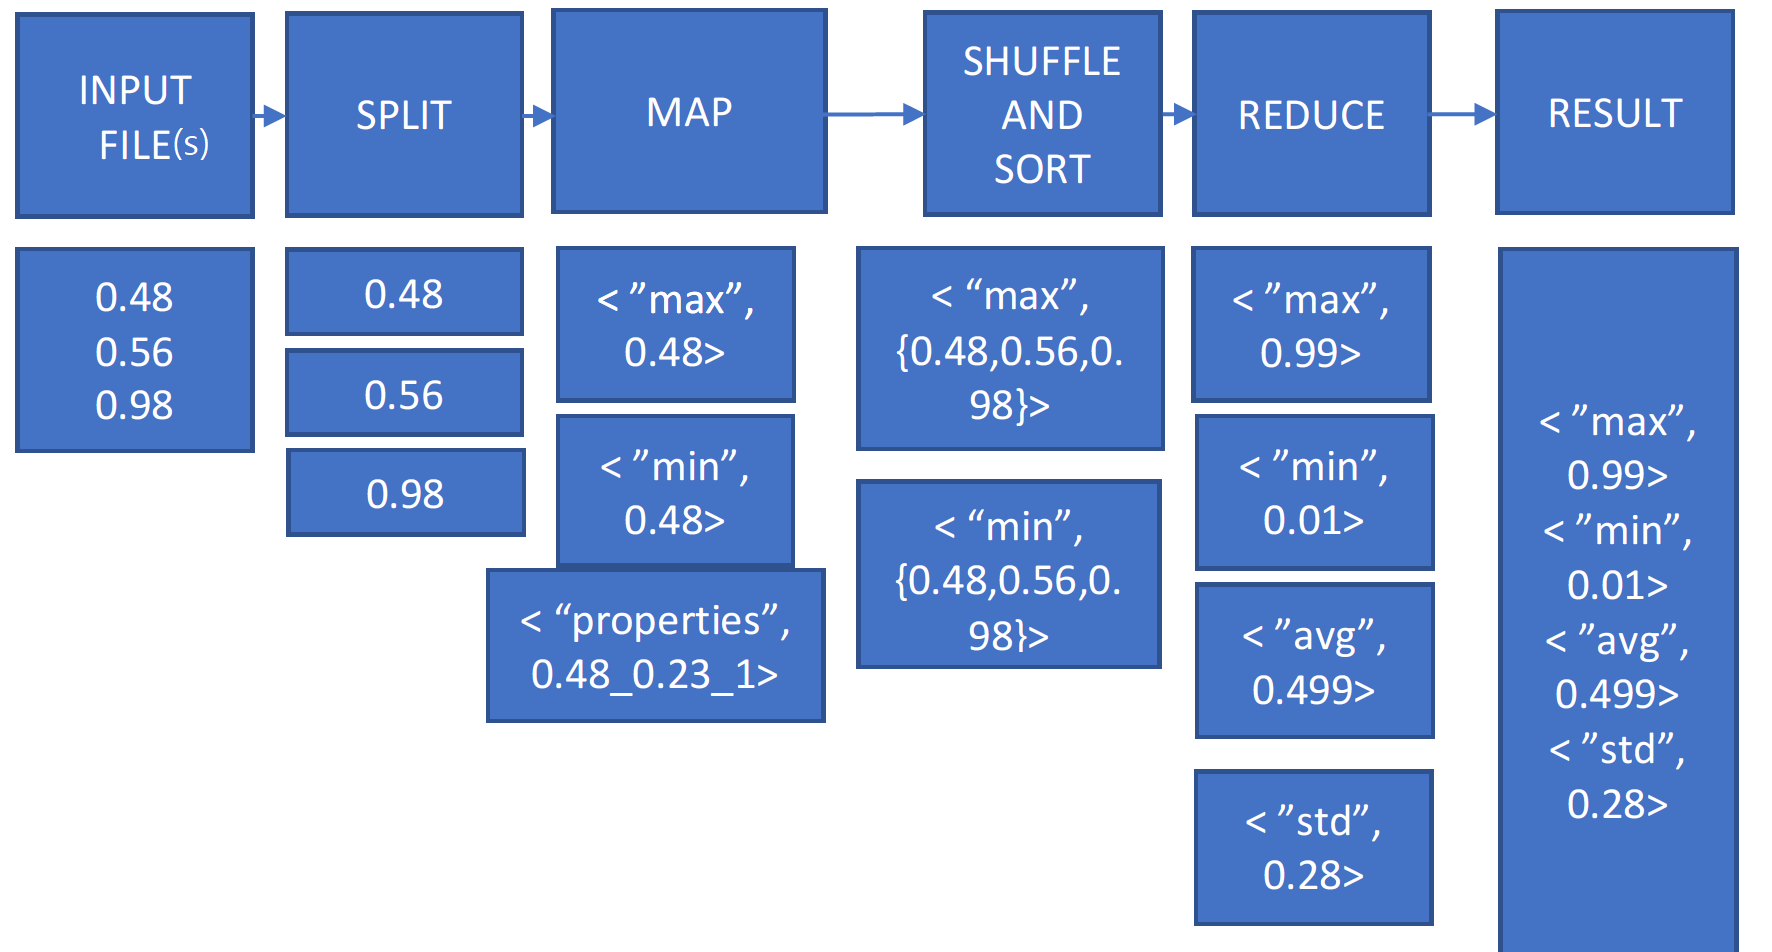
\includegraphics[width=0.9\textwidth]{section/container/images/docker-hadoop-1.png}
 \centering
 \caption{Caption Missing}
\end{figure}

\subsection{Base Location}

The example is available at:

\begin{lstlisting}
cd /cloudmesh/exer1
\end{lstlisting}

\subsection{Input Files}

A test input files are available under
\verb|/cloudmesh/exer1/input_data}|
directory inside of the container. The statistics values for this
input are \textit{Min: 0.20 Max: 19.99 Avg: 9.51 StdDev: 5.55} for all
input files.

10 files contain 55000 lines to process and each line is a random
float point value ranging from 0.2 to 20.0.

\subsection{Compilation}

The source code file name is \textit{MinMaxAvgStd.java} which is
available at \textit{/cloudmesh/exer1/src/exercise/}.

There are three functions in the code \textit{Map, Reduce and Main}
where Map reads each line of a file and updates values to calculate
minimum, maximum values and Reduce collects mappers to produce average
and standard deviation values at last.

\begin{lstlisting}
export HADOOP_CLASSPATH=`$HADOOP_PREFIX/bin/hadoop classpath`
mkdir /cloudmesh/exer1/dest
javac -classpath $HADOOP_CLASSPATH -d /cloudmesh/exer1/dest /cloudmesh/exer1/src/exercise/MinMaxAvgStd.java
\end{lstlisting}

These commands simply prepare compiling the example code and the
compiled class files are generated at the \textit{dest} location.

\subsection{Archiving Class Files}

Jar command tool helps archiving classes in a single file which will be used
when Hadoop runs this example. This is useful because a jar file contains all
necessary files to run a program.

\begin{lstlisting}
jar -cvf exer1.jar -C /cloudmesh/exer1/dest/ /cloudmesh/exer1/
\end{lstlisting}

\subsection{HDFS for Input/Output}

The input files need to be uploaded to HDFS as Hadoop runs this example by
reading input files from HDFS.

\begin{lstlisting}
export PATH=$PATH:/$HADOOP_PREFIX/bin
hadoop fs -mkdir exer1_input
hadoop fs -put input_data/* exer1_input
hadoop fs -ls exer1_input/
\end{lstlisting}

If uploading is completed, you may see file listings like:

\begin{tiny}
\begin{lstlisting}
Found 10 items
-rw-r--r-- 1 root supergroup  13942 2018-02-28 23:16 exer1_input/data_1000.txt
-rw-r--r-- 1 root supergroup 139225 2018-02-28 23:16 exer1_input/data_10000.txt
-rw-r--r-- 1 root supergroup  27868 2018-02-28 23:16 exer1_input/data_2000.txt
-rw-r--r-- 1 root supergroup  41793 2018-02-28 23:16 exer1_input/data_3000.txt
-rw-r--r-- 1 root supergroup  55699 2018-02-28 23:16 exer1_input/data_4000.txt
-rw-r--r-- 1 root supergroup  69663 2018-02-28 23:16 exer1_input/data_5000.txt
-rw-r--r-- 1 root supergroup  83614 2018-02-28 23:16 exer1_input/data_6000.txt
-rw-r--r-- 1 root supergroup  97490 2018-02-28 23:16 exer1_input/data_7000.txt
-rw-r--r-- 1 root supergroup 111451 2018-02-28 23:16 exer1_input/data_8000.txt
-rw-r--r-- 1 root supergroup 125337 2018-02-28 23:16 exer1_input/data_9000.txt
\end{lstlisting}
\end{tiny}

\subsection{Run Program with a Single Input File}

We are ready to run the program to calculate values from text
files. First, we simply run the program with a single input file to
see how it works. \verb|data_1000.txt| contains 1000 lines of
floats, we use this file here.

\begin{lstlisting}
hadoop jar exer1.jar exercise.MinMaxAvgStd exer1_input/data_1000.txt exer1_output_1000
\end{lstlisting}

The command runs with input parameters which indicate a jar file (the
program, exer1.jar), exercise.MinMaxAvgStd (package name.class name),
input file path (\verb|exer1_input/data_1000.txt|) and output file path
(\verb|exer1_output_1000|).

The sample results that the program produces look like this:

\begin{lstlisting}
18/02/28 23:48:50 INFO client.RMProxy: Connecting to ResourceManager at /0.0.0.0:8032
18/02/28 23:48:50 INFO input.FileInputFormat: Total input paths to process: 1
18/02/28 23:48:50 INFO mapreduce.JobSubmitter: number of splits:1
18/02/28 23:48:50 INFO mapreduce.JobSubmitter: Submitting tokens for job: job_1519877569596_0002
18/02/28 23:48:51 INFO impl.YarnClientImpl: Submitted application application_1519877569596_0002
18/02/28 23:48:51 INFO mapreduce.Job: The url to track the job: http://f5e82d68ba4a:8088/proxy/application_1519877569596_0002/
18/02/28 23:48:51 INFO mapreduce.Job: Running job: job_1519877569596_0002
18/02/28 23:48:56 INFO mapreduce.Job: Job job_1519877569596_0002 running in uber mode: false
18/02/28 23:48:56 INFO mapreduce.Job: map 0% reduce 0%
18/02/28 23:49:00 INFO mapreduce.Job: map 100% reduce 0%
18/02/28 23:49:05 INFO mapreduce.Job: map 100% reduce 100%
18/02/28 23:49:05 INFO mapreduce.Job: Job job_1519877569596_0002 completed successfully
18/02/28 23:49:05 INFO mapreduce.Job: Counters: 49
  File System Counters
    FILE: Number of bytes read=81789
    FILE: Number of bytes written=394101
    FILE: Number of read operations=0
    FILE: Number of large read operations=0
    FILE: Number of write operations=0
    HDFS: Number of bytes read=14067
    HDFS: Number of bytes written=86
    HDFS: Number of read operations=6
    HDFS: Number of large read operations=0
    HDFS: Number of write operations=2
  Job Counters
    Launched map tasks=1
    Launched reduce tasks=1
    Data-local map tasks=1
    Total time spent by all maps in occupied slots (ms)=2107
    Total time spent by all reduces in occupied slots (ms)=2316
    Total time spent by all map tasks (ms)=2107
    Total time spent by all reduce tasks (ms)=2316
    Total vcore-seconds taken by all map tasks=2107
    Total vcore-seconds taken by all reduce tasks=2316
    Total megabyte-seconds taken by all map tasks=2157568
    Total megabyte-seconds taken by all reduce tasks=2371584
  Map-Reduce Framework
    Map input records=1000
    Map output records=3000
    Map output bytes=75783
    Map output materialized bytes=81789
    Input split bytes=125
    Combine input records=0
    Combine output records=0
    Reduce input groups=3
    Reduce shuffle bytes=81789
    Reduce input records=3000
    Reduce output records=4
    Spilled Records=6000
    Shuffled Maps =1
    Failed Shuffles=0
    Merged Map outputs=1
    GC time elapsed (ms)=31
    CPU time spent (ms)=1440
    Physical memory (bytes) snapshot=434913280
    Virtual memory (bytes) snapshot=1497260032
    Total committed heap usage (bytes)=402653184
  Shuffle Errors
    BAD_ID=0
    CONNECTION=0
    IO_ERROR=0
    WRONG_LENGTH=0
    WRONG_MAP=0
    WRONG_REDUCE=0
  File Input Format Counters
    Bytes Read=13942
  File Output Format Counters
    Bytes Written=86

\end{lstlisting}

The second line of the following logs indicates that the number of
input files is 1.

\subsection{Result for Single Input File}

We reads results from HDFS by:

\begin{lstlisting}
doop fs -cat exer1_output_1000/part-r-00000
\end{lstlisting}

The sample output looks like:

\begin{lstlisting}
Max: 19.9678704297
Min: 0.218880718983
Avg: 10.225467263249385
Std: 5.679809322880863
\end{lstlisting}

\subsection{Run Program with Multiple Input Files}

The first run was done pretty quickly (1440 milliseconds took
according to the sample result above) because the input file size was
small (1,000 lines) and it was a single file. We provides more input
files with a larger size (2,000 to 10,000 lines). Input files are
already uploaded to HDFS. We simply run the program again with a
slight change in the parameters.

\begin{lstlisting}
hadoop jar exer1.jar exercise.MinMaxAvgStd exer1_input/ exer1_output_all
\end{lstlisting}

The command is almost same except that an input path is a directory
and a new output directory. Note that every time that you run this
program, the output directory will be created which means that you
have to provide a new directory name unless you delete it.

The sample output messages look like the following which is almost
identical compared to the previous run except that this time the
number of input files to process is 10, see the line two below:

\begin{lstlisting}
18/02/28 23:17:18 INFO client.RMProxy: Connecting to ResourceManager at /0.0.0.0:8032
18/02/28 23:17:18 INFO input.FileInputFormat: Total input paths to process: 10
18/02/28 23:17:18 INFO mapreduce.JobSubmitter: number of splits:10
18/02/28 23:17:18 INFO mapreduce.JobSubmitter: Submitting tokens for job: job_1519877569596_0001
18/02/28 23:17:19 INFO impl.YarnClientImpl: Submitted application application_1519877569596_0001
18/02/28 23:17:19 INFO mapreduce.Job: The url to track the job: http://f5e82d68ba4a:8088/proxy/application_1519877569596_0001/
18/02/28 23:17:19 INFO mapreduce.Job: Running job: job_1519877569596_0001
18/02/28 23:17:24 INFO mapreduce.Job: Job job_1519877569596_0001 running in uber mode: false
18/02/28 23:17:24 INFO mapreduce.Job: map 0% reduce 0%
18/02/28 23:17:32 INFO mapreduce.Job: map 40% reduce 0%
18/02/28 23:17:33 INFO mapreduce.Job: map 60% reduce 0%
18/02/28 23:17:36 INFO mapreduce.Job: map 70% reduce 0%
18/02/28 23:17:37 INFO mapreduce.Job: map 100% reduce 0%
18/02/28 23:17:39 INFO mapreduce.Job: map 100% reduce 100%
18/02/28 23:17:39 INFO mapreduce.Job: Job job_1519877569596_0001 completed successfully
18/02/28 23:17:39 INFO mapreduce.Job: Counters: 49
  File System Counters
    FILE: Number of bytes read=4496318
    FILE: Number of bytes written=10260627
    FILE: Number of read operations=0
    FILE: Number of large read operations=0
    FILE: Number of write operations=0
    HDFS: Number of bytes read=767333
    HDFS: Number of bytes written=84
    HDFS: Number of read operations=33
    HDFS: Number of large read operations=0
    HDFS: Number of write operations=2
  Job Counters
    Launched map tasks=10
    Launched reduce tasks=1
    Data-local map tasks=10
    Total time spent by all maps in occupied slots (ms)=50866
    Total time spent by all reduces in occupied slots (ms)=4490
    Total time spent by all map tasks (ms)=50866
    Total time spent by all reduce tasks (ms)=4490
    Total vcore-seconds taken by all map tasks=50866
    Total vcore-seconds taken by all reduce tasks=4490
    Total megabyte-seconds taken by all map tasks=52086784
    Total megabyte-seconds taken by all reduce tasks=4597760
  Map-Reduce Framework
    Map input records=55000
    Map output records=165000
    Map output bytes=4166312
    Map output materialized bytes=4496372
    Input split bytes=1251
    Combine input records=0
    Combine output records=0
    Reduce input groups=3
    Reduce shuffle bytes=4496372
    Reduce input records=165000
    Reduce output records=4
    Spilled Records=330000
    Shuffled Maps =10
    Failed Shuffles=0
    Merged Map outputs=10
    GC time elapsed (ms)=555
    CPU time spent (ms)=16040
    Physical memory (bytes) snapshot=2837708800
    Virtual memory (bytes) snapshot=8200089600
    Total committed heap usage (bytes)=2213019648
  Shuffle Errors
    BAD_ID=0
    CONNECTION=0
    IO_ERROR=0
    WRONG_LENGTH=0
    WRONG_MAP=0
    WRONG_REDUCE=0
  File Input Format Counters
    Bytes Read=766082
  File Output Format Counters
    Bytes Written=84
\end{lstlisting}


\subsection{Result for Multiple Files}

\begin{lstlisting}
hadoop fs -cat exer1_output_all/part-r-00000
\end{lstlisting}

The expected result looks like:

\begin{lstlisting}
Max: 19.999191254
Min: 0.200268613863
Avg: 9.514884854468903
Std: 5.553921579413547
\end{lstlisting}

\section{Conclusion}

The example program of calculating some values by reading multiple
files shows how Map/Reduce is written by a Java programming language
and how Hadoop runs its program using HDFS. We also observed the one
of benefits using Docker container which is that the hassle of
configuration and installation of Hadoop is not necessary anymore.



% chktex-file 1
% chktex-file 18
% chktex-file 25

\FILENAME

\section{Apache Spark with Docker}\label{s:apache-spark-with-docker}

\subsection{Pull Image from Docker
Repository}

We use a Docker image from Docker Hub:
(https://hub.docker.com/r/sequenceiq/spark/) This repository contains a
Docker file to build a Docker image with Apache Spark and Hadoop Yarn.

\begin{lstlisting}
docker pull sequenceiq/spark:1.6.0
\end{lstlisting}

\subsection{Running the Image}

In this step, we will launch a Spark container.

\subsubsection{Running interactively}

\begin{lstlisting}
docker run -it -p 8088:8088 -p 8042:8042 -h sandbox sequenceiq/spark:1.6.0 bash
\end{lstlisting}

\subsubsection{Running in the
background}

\begin{lstlisting}
docker run -d -h sandbox sequenceiq/spark:1.6.0 -d
\end{lstlisting}

\subsection{Run Spark}

After a container is launched, we can run Spark in the following two
modes: (1) yarn-client and (2) yarn-cluster. The differences between the
two modes can be found here:
https://spark.apache.org/docs/latest/running-on-yarn.html

\subsubsection{Run Spark in Yarn-Client
Mode}

\begin{lstlisting}
spark-shell --master yarn-client --driver-memory 1g --executor-memory 1g --executor-cores 1
\end{lstlisting}

\subsubsection{Run Spark in Yarn-Cluster
Mode}

\begin{lstlisting}
spark-submit --class org.apache.spark.examples.SparkPi --master yarn-client --driver-memory 1g --executor-memory 1g --executor-cores 1 $SPARK_HOME/lib/spark-examples-1.6.0-hadoop2.6.0.jar
\end{lstlisting}

\subsection{Observe Task Execution from Running Logs of SparkPi}

Let us observe Spark task execution by adjusting the parameter of
SparkPi and the Pi result from the following two commands.

\begin{lstlisting}
spark-submit --class org.apache.spark.examples.SparkPi --master yarn-client --driver-memory 1g --executor-memory 1g --executor-cores 1 $SPARK_HOME/lib/spark-examples-1.6.0-hadoop2.6.0.jar 10
\end{lstlisting}

\begin{lstlisting}
spark-submit --class org.apache.spark.examples.SparkPi --master yarn-client --driver-memory 1g --executor-memory 1g --executor-cores 1 $SPARK_HOME/lib/spark-examples-1.6.0-hadoop2.6.0.jar 10000
\end{lstlisting}

\subsection{Write a Word-Count Application with Spark RDD}

Let us write our own word-count with Spark RDD. After the shell has been
started, copy and paste the following code in console line by line.

\subsubsection{Launch Spark Interactive Shell}

\begin{lstlisting}
spark-shell --master yarn-client --driver-memory 1g --executor-memory 1g --executor-cores 1
\end{lstlisting}

\subsubsection{Program in Scala}

\begin{lstlisting}
val textFile = sc.textFile("file:///etc/hosts")
val words = textFile.flatMap(line => line.split("\\s+"))
val counts = words.map(word => (word, 1)).reduceByKey(_ + _)
counts.values.sum()
\end{lstlisting}

\subsubsection{Launch PySpark Interactive Shell}

\begin{lstlisting}
pyspark --master yarn-client --driver-memory 1g --executor-memory 1g --executor-cores 1
\end{lstlisting}

\subsubsection{Program in Python}

\begin{lstlisting}
textFile = sc.textFile("file:///etc/hosts")
words = textFile.flatMap(lambda line:line.split())
counts = words.map(lambda word:(word, 1)).reduceByKey(lambda x,y: x+y)
counts.map(lambda x:x[1]).sum()
\end{lstlisting}

\subsection{Docker Spark Examples}

\subsubsection{K-Means Example}

First we need to pull the image from the Docker Hub :

\begin{lstlisting}
docker pull sequenceiq/spark-native-yarn
\end{lstlisting}

It will take sometime to download the image. Now we have to run docker
spark image interactively.

\begin{lstlisting}
docker run -i -t -h sandbox sequenceiq/spark-native-yarn /etc/bootstrap.sh -bash
\end{lstlisting}

This will take you to the interactive mode.

Let's run a sample KMeans example. This is already built with Spark.

Here we specify the data data set from a local folder inside the image
and we run the sample class KMeans in the sample package. The sample
data set used is inside the sample-data folder. Spark has it's own
format for machine learning datasets. Here the kmeans\_data.txt file
contains the KMeans dataset.

\begin{lstlisting}
./bin/spark-submit --class sample.KMeans --master execution-context:org.apache.spark.tez.TezJobExecutionContext --conf update-classpath=true ./lib/spark-native-yarn-samples-1.0.jar /sample-data/kmeans_data.txt
\end{lstlisting}

If you run this successfully, you can get an output as shown here.

\begin{lstlisting}
Finished iteration (delta = 0.0)
Final centers:
DenseVector(0.15000000000000002, 0.15000000000000002, 0.15000000000000002)
DenseVector(9.2, 9.2, 9.2)
DenseVector(0.0, 0.0, 0.0)
DenseVector(9.05, 9.05, 9.05)
\end{lstlisting}

\subsubsection{Join Example}

Run the following command to do a sample join operation on a given
dataset. Here we use two datasets, namely join1.txt and join2.txt. Then
we perform the join operation that we discussed in the theory section.

\begin{lstlisting}
./bin/spark-submit --class sample.Join --master execution-context:org.apache.spark.tez.TezJobExecutionContext --conf update-classpath=true ./lib/spark-native-yarn-samples-1.0.jar /sample-data/join1.txt /sample-data/join2.txt
\end{lstlisting}

\subsubsection{Word Count}

In this example the wordcount.txt will used to do the word count using
multiple reducers. Number 1 at the end of the command determines the
number of reducers. As spark can run multiple reducers, we can specify
the number as a parameter to the programme.

\begin{lstlisting}
./bin/spark-submit --class sample.WordCount --master execution-context:org.apache.spark.tez.TezJobExecutionContext --conf update-classpath=true ./lib/spark-native-yarn-samples-1.0.jar /sample-data/wordcount.txt 1
\end{lstlisting}

\subsection{Interactive Examples}

Here we need a new image to work on. Let's run the following command.
This will pull the necessary repositories from docker hub, as we don't
have most of the dependencies related to it. This can take a few minutes
to download everything.

\begin{lstlisting}
docker run -it-p 8888:8888 -v $PWD:/cloudmesh/spark --name spark jupyter/pyspark-notebook
\end{lstlisting}

Here you will get the following output in the terminal.

\begin{figure}[htbp]
\centering
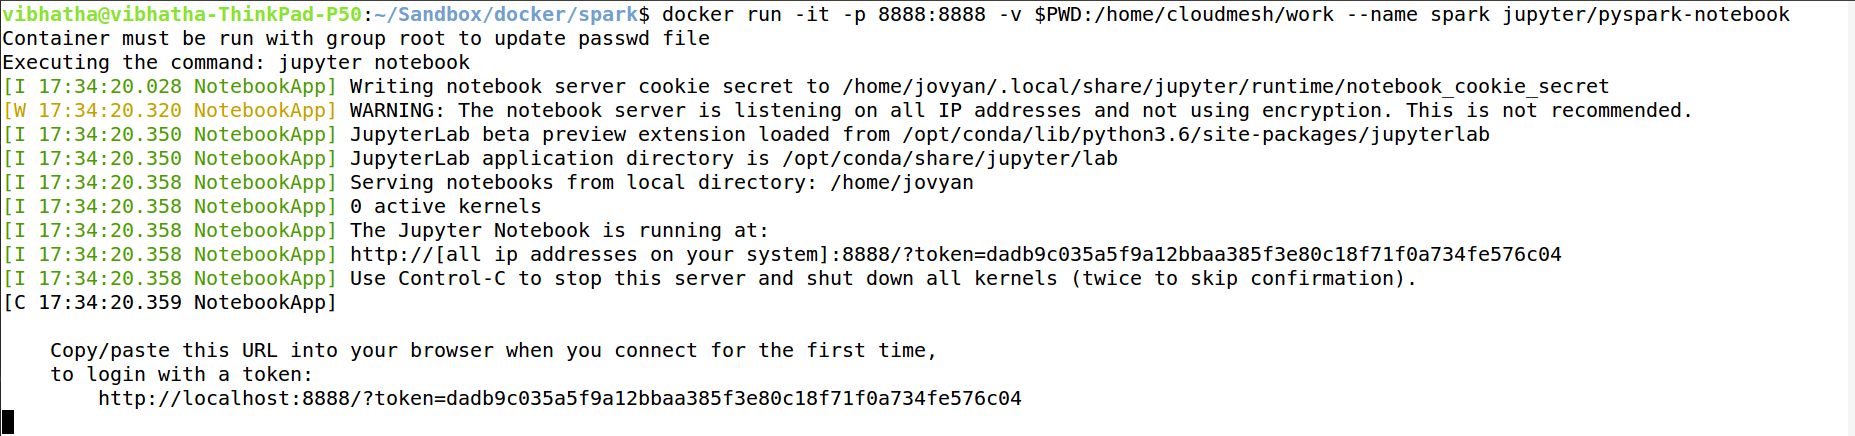
\includegraphics[width=1.0\textwidth]{images/docker-spark-jupyter.png}
\caption{Terminal Output}
\end{figure}

Please copy the url shown at the end of the terminal output and go to
that url in the browser.

You will see the following output in the browser, (Use Google Chrome)

\begin{figure}[htbp]
\centering
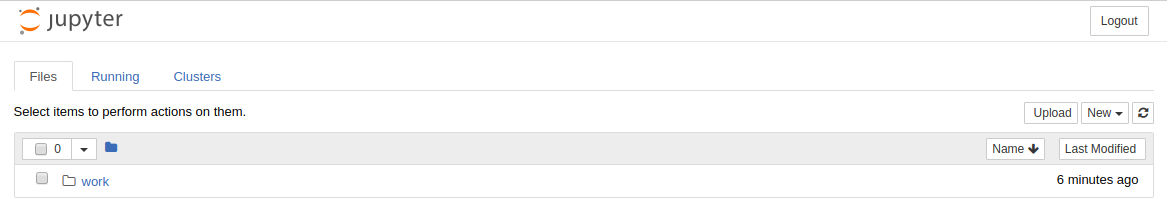
\includegraphics[width=1.0\textwidth]{images/docker-spark-jup-1.png}
\caption{Jupyter Notebook in Browswer}
\end{figure}

First navigate to the work folder. Let us create a new python file here.
Click python3 in the new menu.

\begin{figure}[htbp]
\centering
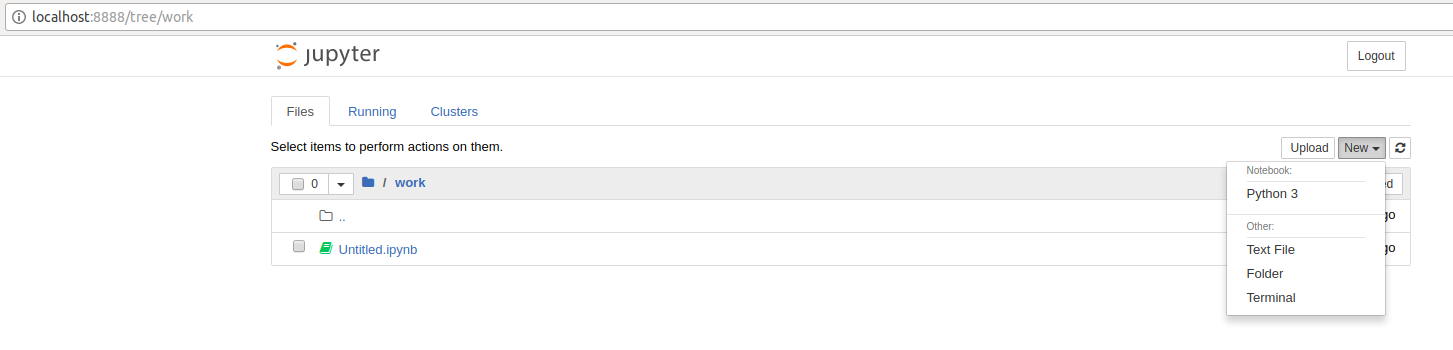
\includegraphics[width=1.0\textwidth]{images/docker-spark-jup-2.png}
\caption{Create a new python file}
\end{figure}

Now add the following content in the new file. In Jupyter notebook, you
can enter a python command or python code and press

\begin{lstlisting}
SHIFT + ENTER
\end{lstlisting}

This will run the code interactively.

Now let's create the following content.

\begin{figure}[htbp]
\centering
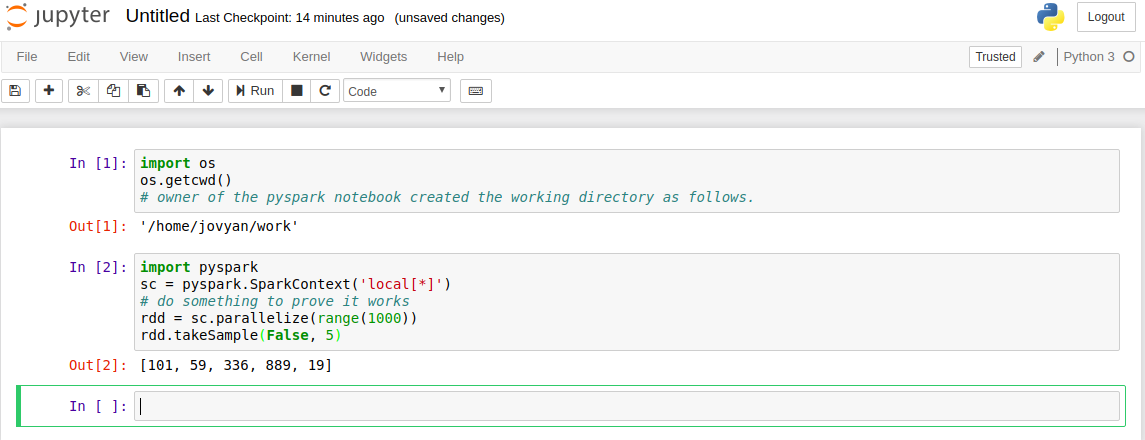
\includegraphics[width=1.0\textwidth]{images/docker-spark-jup-3.png}
\caption{Create a new python file}
\end{figure}

Now let us do the following.

In the following stage we configure spark context and import the
necessary files.

\begin{figure}[htbp]
\centering
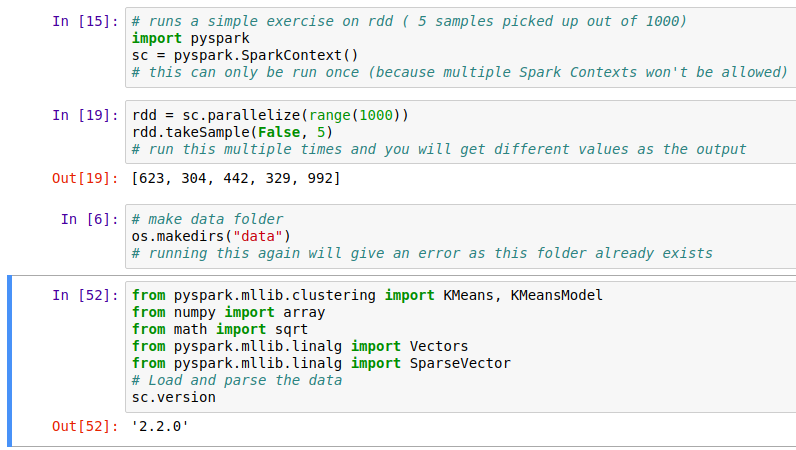
\includegraphics[width=0.7\textwidth]{images/docker-spark-tut-1.png}
\caption{Initial Spark Program}
\end{figure}

Next stage we use sample data set by creating them in form of an array
and we train the kmeans algorithm.

\begin{figure}[htbp]
\centering
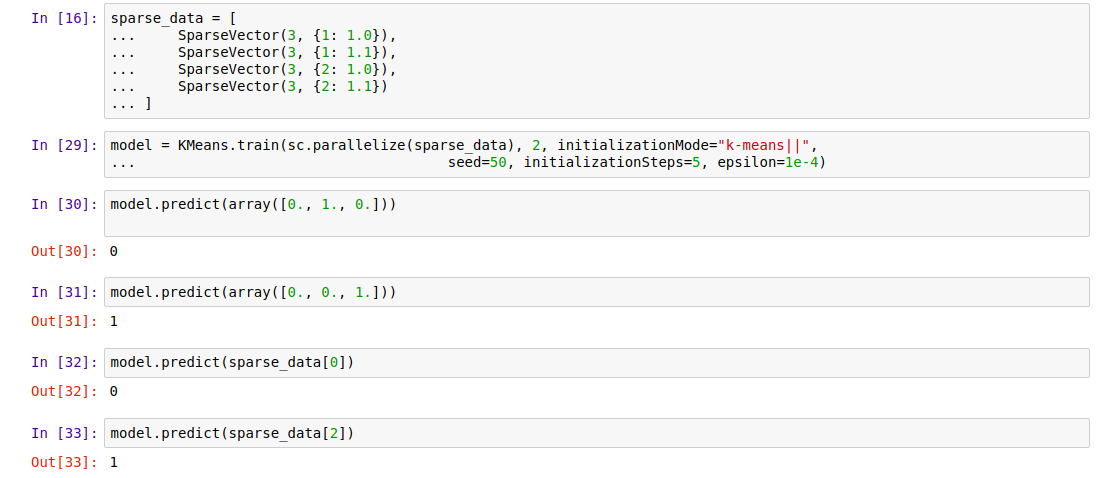
\includegraphics[width=1.0\textwidth]{images/docker-spark-tut-4.png}
\caption{Train KMeans}
\end{figure}

In the final stage we put sample values and check the predictions on the
cluster. In addition to that feed the data using SparseVector format and
we add the kmeans initialization mode, the error margin and the
parallelization. We put the step size as 5 for this example. In the
previous one we didn't specify any parameters.

The predict term predicts the cluster id which it belongs to.

\begin{figure}[htbp]
\centering
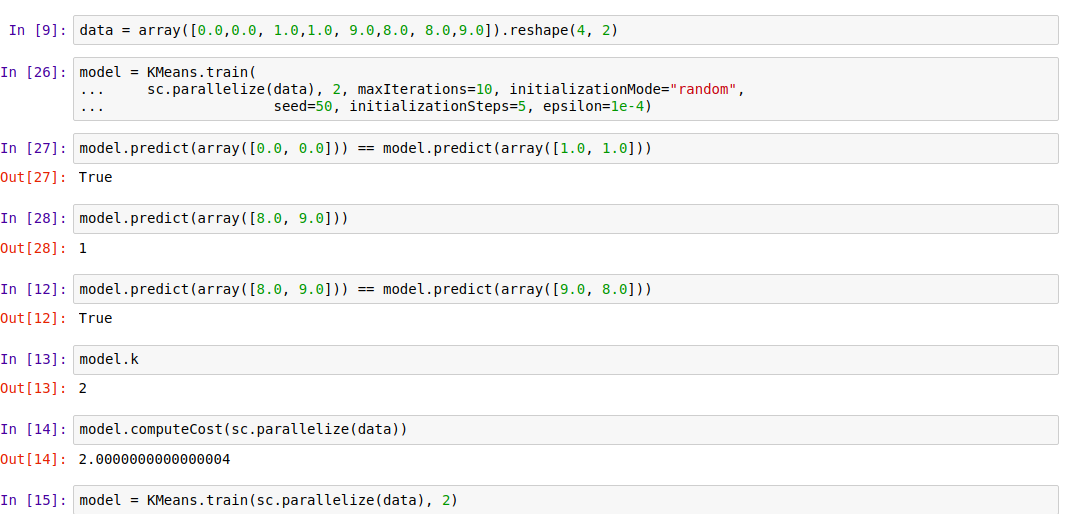
\includegraphics[width=1.0\textwidth]{images/docker-spark-tut-5.png}
\caption{Predict KMeans Clusters-1}
\end{figure}

Then in the following way you can check whether two data points belong
to one cluster or not.

\begin{figure}[htbp]
\centering
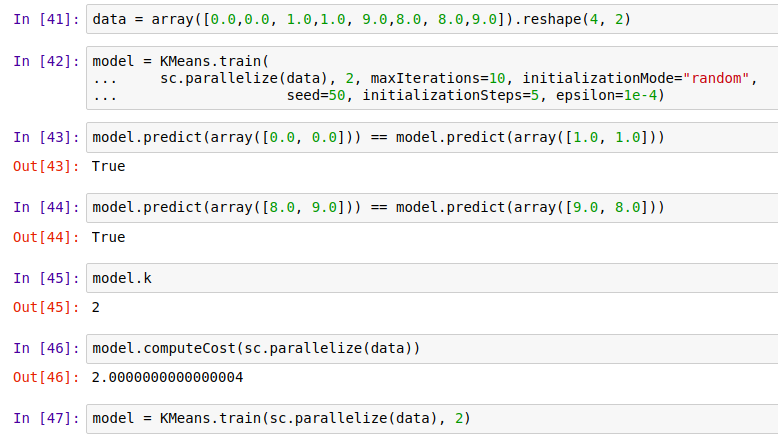
\includegraphics[width=1.0\textwidth]{images/docker-spark-tut-2.png}
\caption{Predict KMeans Clusters-2}
\end{figure}
 
\begin{figure}[htbp]
\centering
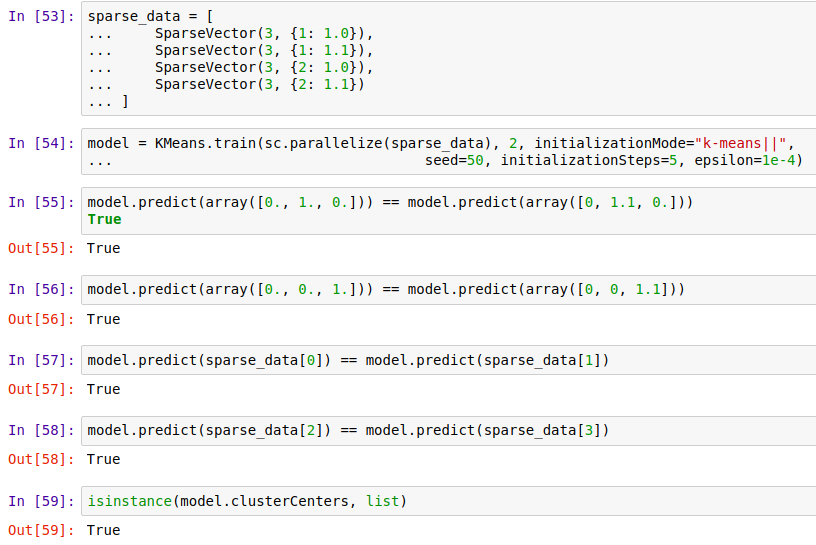
\includegraphics[width=1.0\textwidth]{images/docker-spark-tut-3.png}
\caption{Predict KMeans Clusters-3}
\end{figure}

\subsubsection{Stop Docker Container}

\begin{lstlisting}
docker stop spark
\end{lstlisting}

\subsubsection{Start Docker Container
Again}

\begin{lstlisting}
docker start spark
\end{lstlisting}

\subsubsection{Remove Docker Container}

\begin{lstlisting}
docker rm spark
\end{lstlisting}

% chktex-file 1

\chapter{Draft: Container}

\FILENAME




\section{Container Orchestration Tools: Compare Kubernetes vs Docker Swarm}

\URL{https://platform9.com/blog/compare-kubernetes-vs-docker-swarm/}

\section{Gentle introduction to Containers}

\URL{https://www.slideshare.net/jpetazzo/introduction-docker-linux-containers-lxc}

\section{Tutorialspoint}

\URL{https://www.tutorialspoint.com/docker/index.htm}

\URL{https://www.tutorialspoint.com/docker/docker_tutorial.pdf}

\URL{https://www.tutorialspoint.com/docker/docker_pdf_version.htm}


\chapter{Exercises}

\section{Docker Swarm Tutorial}

\begin{exercise}

  Develop a tutorial that deploys a Docker Swarm cluster on a number
  of ubuntu machines. Note that this may actually be easier as docker
  and docker swarm are distributed with recent versions of
  ubuntu. Just in case we are providing a link to an effort we found
  to install docker swarm. However we have not checked it or
  identified if it is useful.
 
  \URL{https://rominirani.com/docker-swarm-tutorial-b67470cf8872}

\end{exercise}


\section{Docker Swarm on Google Compute Engine}

\begin{exercise}
  Develop a tutorial that deploys a Docker Swarm cluster on Google
  Compute Engine. Note that this may actually be easier as docker
  and docker swarm are distributed with recent versions of
  ubuntu. Just in case we are providing a link to an effort we found
  to install docker swarm. However we have not checked it or
  identified if it is useful.

  \URL{https://rominirani.com/docker-swarm-on-google-compute-engine-364765b400ed}

\end{exercise}

\section{Single Node Hadoop}

\begin{exercise}

At

\url{https://hadoop.apache.org/docs/current/hadoop-project-dist/hadoop-common/SingleCluster.html}

you will find a comprehensive installation instruction that sets up a
hadoop cluster on a single node. 

(a) Create a Dockerfile that deploys hadoop in a container

(b) Develop sample applications and tests to test your cluster. You
can use wordcount or similar.

\end{exercise}


\section{Single Node Hadoop}

\begin{exercise}

At

\url{https://hadoop.apache.org/docs/r3.0.0/hadoop-project-dist/hadoop-common/ClusterSetup.html}

you will find a comprehensive installation instruction that sets up a
hadoop cluster in a distributed environment, can you use this set of
instructions aor identify other resources on the internet that allow
the creation of a hadoop cluster on kubernetes. You can use docker
compose for this.


(a) Create docker compose and Dockerfiles that deploys hadoop in
kubernetes

(b) Develop sample applications and tests to test your cluster. You
can use wordcount or similar.

\end{exercise}



\section{Spark Cluster}

\begin{exercise}

Develop a high quality tutorial that installes a spark cluster in
kubernetes. Test your deployment on minikube but also Futuresystems
echo.

You may want to get inspired from the talk \textit{Scalable Spark
  Deployment using Kubernetes}:

\URL{http://blog.madhukaraphatak.com/scaling-spark-with-kubernetes-part-1/}
\URL{http://blog.madhukaraphatak.com/scaling-spark-with-kubernetes-part-2/}
\URL{http://blog.madhukaraphatak.com/scaling-spark-with-kubernetes-part-3/}
\URL{http://blog.madhukaraphatak.com/scaling-spark-with-kubernetes-part-4/}
\URL{http://blog.madhukaraphatak.com/scaling-spark-with-kubernetes-part-5/}
\URL{http://blog.madhukaraphatak.com/scaling-spark-with-kubernetes-part-6/}
\URL{http://blog.madhukaraphatak.com/scaling-spark-with-kubernetes-part-7/}
\URL{http://blog.madhukaraphatak.com/scaling-spark-with-kubernetes-part-8/}
\URL{http://blog.madhukaraphatak.com/scaling-spark-with-kubernetes-part-9/}

Make sure you do not plagiarize.

\end{exercise}



%\chapterimage{pigeon.jpeg}
\chapter{MQTT}
\label{c:mqtt}
%
With the increase importance of cloud computing and the increased
number of edge devices and their applications, such as sensor
networks, it is crucial to enable fast communication between the
sensing devices and actuators, which may not be directly connected, as
well as cloud services that analyze the data. To allow services that
are built on different software and hardware platforms to communicate,
a data agnostic, fast and service is needed. In addition to
communication, the data generated by these devices, services, and
sensors must be analyzed. Security aspects to relay this data is
highly important. We will introduce a service called MQTT, which is a
common, easy to use, queuing protocol that helps meet these
requirements.  


\section{Introduction}

As Cloud Computing and Internet of Things (IoT) applications and
sensor networks become commonplace and more and more devices are being
connected, there is an increased need to allow these devices to
communicate quickly and securely. In many cases these edge devices
have very limited memory and need to conserve power. The computing
power on some of these devices is so limited that the sensory data
need to be analyzed remotely. Furthermore, they may not even have
enough computing capacity to process traditional HTTP web requests
efficiently~\cite{mqtt-vs-http}\cite{hivemq-website} or these traditional
Web-based services are too resource hungry. Monitoring the state of a
remotely located sensor using HTTP would require sending requests and
receiving responses to and from the device frequently, which may not
be efficient on small circuits or embedded chips on edge computing
sensors~\cite{mqtt-vs-http}.

Message Queue Telemetry Transport (MQTT) is a lightweight machine to
machine (M2M) messaging protocol, based on a client/server 
publish-subscribe model. It provides a a simple service allowing us to
communicate between sensors, and services based on a subscription
model.

MQTT was first developed in 1999 to connect oil pipelines
\cite{hivemq-website}. The protocol has been designed to be used on
top of TCP/IP protocol in situations where network bandwidth, and
available memory are limited allowing low power usage. However, as it
is implemented on top of TCP/IP it is reliable in contrast to other
protocols such as UDP. It allows efficient transmission of
data to various devices listening for the same event, and is scalable
as the number of devices increase
\cite{mqtt-wiki}\cite{mqtt-official}.

The current support for MQTT is conducted as part of the Eclipse Paho
project~\cite{eclipse-mosquitto}.  As MQTT is a protocol many
different clients in various languages exist.  This includes languages
such as Python, C, Java, Lua, and many more.

The current standard of MQTT is available at 

\url{http://docs.oasis-open.org/mqtt/mqtt/v3.1.1/os/mqtt-v3.1.1-os.pdf}

\section{Publish Subscribe Model}

MQTT works via a publish-subscribe model that contains 3 entities: (1) a
publisher, that sends a message, (2) a broker, that maintains queue of all
messages based on topics and (3) multiple subscribers that subscribe to
various topics they are interested in~\cite{how-mqtt-works}.

This allows for decoupling of functionality at various levels. The
publisher and subscriber do not need to be close to each other and do
not need to know each others identity. They need only to know the
broker, as the publisher and the subscribers do not have to be running
either at the same time nor on the same hardware
\cite{hivemq-details}.

Ready to use implementation exist to be deployed as brokers in the
users application frameworks. A broker is a service that relays
information between the client and servers. Common brokers include the
open source Mosquito broker~\cite{mqtt-official} and the Eclipse Phao
MQTT Broker~\cite{eclipse-mosquitto}.


\subsection{Topics}

MQTT implements a hierarchy of topics that are relates
to all messages. These topics are recognised by strings separated by a
forward-slash (/), where each part represents a different topic
level. This is a common model introduced in file systems but also in
internet URLs. 

A topic looks therefore as follows: \textit{topic-level0/topic-level1/topic-level2}.



Subscribers can subscribe to different topics via the broker.
Subscribing to \textit{topic-level0} allows the subscriber to receive all
messages that are associated with topics that start with {\em
  topic-level0}. This allows subscribers to filter what messages to
receive based on the topic hierarchy. Thus, when a publisher publishes
a message related to a topic to the broker, the message is forwarded
to all the clients that have subscribed to the topic of the message or
a topic that has a lower depth of hierarchy~\cite{hivemq-details}
\cite{how-mqtt-works}.

This is different from traditional point-to-point message queues as
the message is forwarded to multiple subscribers, and allows for
flexibility of dealing with subscribed topics not only on the server
but also on the subscriber side~\cite{hivemq-details}. The basic steps
in a MQTT client subscriber application include to (1) connect to the broker,
(2) subscribe to some topics, (3) wait for messages and (4) perform the
appropriate action when a certain message is received
\cite{mqtt-wiki}.
 
\subsection{Callbacks}

One of the advantages of using MQTT is that it supports
asynchronous behaviour with the help of callbacks. Both the publisher
and subscriber can use non-blocking callbacks to act upon message exchanges.
\cite{hivemq-details}\cite{python-paho-mqtt}.

For example, the paho-mqtt package for python provides callbacks
methods including \verb|on-connect()|, \verb|on-message()| and
\verb|on-disconnect()|, which are invoked when the connection to the
broker is complete, a message is received from the broker, and when
the client is disconnected from the broker respectively. These methods
are used in conjunction with the \verb|loop-start()| and \verb|loop-end()| methods
which start and end an asynchronous loop that listens for these events
invoking the relevant callbacks. Hence it frees the services to perform
other tasks~\cite{python-paho-mqtt} when no messages are available,
thus reducing overhead.

\subsection{Quality of Service}

MQTT has been designed to be flexible allowing for the change of
quality of service (QoS) as desired by the application. Three basic
levels of QoS are supported by the protocol:  Atmost-once (QoS level
0), Atleast-once (QoS level 1) and Atmost-once (QoS level 2)
\cite{hivemq-qos,python-paho-mqtt}.

\begin{description}

\item[QoS level 0:] The QoS level of 0 is used in applications where
  some dropped messages may not affect the application. Under this QoS
  level, the broker forwards a message to the subscribers only once
  and does not wait for any
  acknowledgement~\cite{hivemq-qos}\cite{python-paho-mqtt}.

\item[QoS Level 1:] The QoS level of 1 is used in situations where the
  delivery of all messages is important and the subscriber can handle
  duplicate messages. Here the broker keeps on resending the message
  to a subscriber after a certain timeout until the first
  acknowledgement is received.

\item[QoS Level 3:] A QoS level of 3 is used in cases where all
  messages must be delivered and no duplicate messages should be
  allowed. In this case the broker sets up a handshake with the
  subscriber to check for its availability before sending the
  message~\cite{hivemq-qos,python-paho-mqtt}.

\end{description}

The various levels of quality of service allow the use of this
protocol with different service level expectations.

\section{Secure MQTT Services}

MQTT specification uses TCP/IP to deliver the messaged to the
subscribers, but it does not provide security by default to enable
resource constrained IoT devices. ``It allows the use of username and
password for authentication, but by default this information is sent
as plain text over the network, making it susceptible to man-in-the
middle attacks''
\cite{iot-design-mqtt-security,mqtt-sec-ssl}. Therefore, to support
sensitive applications additional security measures need to be
integrated through other means. This may include for example the use
of Virtual Private Networks (VPNs), Transport Layer Security, or
application layer security~\cite{mqtt-sec-ssl}.

\subsection{Using TLS/SSL}

Transport Layer Security (TLS) and Secure Sockets Layer (SSL) are
cryptographic protocols that establish a the identity of the server
and client with the help of a handshake mechanism which uses trust
certificates to establish identities before encrypted communication
can take place~\cite{ibm-mqtt-security}. If the handshake is not
completed for some reason, the connection is not established and no
messages are exchanged~\cite{mqtt-sec-ssl}. ``Most MQTT brokers
provide an option to use TLS instead of plain TCP and port 8883 has
been standardized for secured MQTT connections''
\cite{iot-design-mqtt-security}.

Using TLS/SSL security however comes at an additional cost. If the
connections are short-lived then most of the time is spent in
verifying the security of the handshake itself, which in addition to
using time for encryption and decryption, may take up few
kilobytes of bandwidth. In case the connections are short-lived,
temporary session IDs and session tickets can be used as alternative to resume a
session instead of repeating the handshake process. If the connections
are long term, the overhead of the handshake is negligible and TLS/SSL
security should be used
\cite{iot-design-mqtt-security,mqtt-sec-ssl}.

\subsection{Using OAuth}

OAuth is an open protocol that allows access to a resource without
providing unencrypted credentials to the third party. Although MQTT
protocol itself does not include authorization, many MQTT brokers
include authorization as an additional feature
\cite{ibm-mqtt-security}. OAuth2.0 uses JSON Web Tokens which contain
information about the token ans the user and are signed by a trusted
authorization server~\cite{hivemq-security-oauth}.

When connecting to the broker this token can be used to check whether
the client is authorised to connect at this time or not. Additionally
the same validations can be used when publishing or subscribing to the
broker. The broker may use a third party resource such as LDAP
(lightweight directory access protocol) to look up authorizations for
the client~\cite{hivemq-security-oauth}. Since there can be a large
number of clients and it can become impractical to authorize everyone,
clients may be grouped and the authorizations may be checked for each
group~\cite{ibm-mqtt-security}.
  
\section{Integration with Other Services}

As the individual IoT devices perform their respective functions in
the sensor network, a lot of data is generated which needs to be
processed. MQTT allows easy integration with other services, that have
been designed to process this data. Let us provide some examples of
MQTT integration into other Services.

\begin{description}

\item[Apache Storm.] Apache storm is a distributed processing system
  that allows real time processing of continuous data streams, much
  like Hadoop works for batch processing~\cite{apache-storm}. Apache
  storm can be easily integrated with MQTT as shown
  in~\cite{apache-storm-mqtt} to get real time data streams and allow
  analytics and online machine learning in a fault tolerant
  manner~\cite{apache-storm-wiki}.

\item [ELK stack.]  ELK stack (elastic-search, logstash and kibana) is
  an opensource project designed for scalability which contains three
  main software packages, the \textit{elastic-search} search and
  analytics engine, \textit{logstash} which is a data collection
  pipeline and \textit{kibana} which is a visualization
  dashboard~\cite{elk-stack}. Data from an IoT network can be
  collected, analysed and visualized easily with the help of the ELK
  stack as shown in~\cite{mqtt-elasticsearch-setup} and~\cite{kibana-mqtt-analysis}.


\end{description}

\section{MQTT in Production}

When using optimized MQTT broker services, MQTT can be utilized for
enterprise and production environments. A good example is the use of
EMQ (Erlang MQTT Broker) that provides a highly scalable, distributed
and reliable MQTT broker for enterprise-grade applications
\cite{erlang-mqtt-broker}.


\section{Simple Usecase}

In this example we are demonstrating how to set up a MQTT broker, a
client and a subscriber.

% We are running the program in three
%terminals to showcase the log or output of each server.

\URL{https://github.com/bigdata-i523/sample-hid000/tree/master/experiment/mqtt}

A test program that starts a MQTT broker and client is provided next,
showcasing how simple the interactions are while using a higher level
API such as provided through the python client library of Paho.

\begin{lstlisting}
import paho.mqtt.client as mqtt 
import time


def on_message(client, userdata, message):
    print("message received ", str(message.payload.decode("utf-8")))
    print("message topic=", message.topic)
    print("message qos=", message.qos)
    print("message retain flag=", message.retain)

def on_log(client, userdata, level, buf):
    print("log: ",buf)

broker_address="localhost"    
# broker_address="test.mosquitto.org"
# broker_address="broker.hivemq.com"
# broker_address="iot.eclipse.org"

print("creating new instance")
client = mqtt.Client("i523") #create new instance
client.on_log=on_log
client.on_message=on_message #attach function to callback

print("connecting to broker")
client.connect(broker_address) #connect to broker
client.loop_start() #start the loop

print("Subscribing to topic","robot/leds/led1")
client.subscribe("robot/leds/led1")

print("Publishing message to topic","robot/leds/led1")
client.publish("robot/leds/led1","OFF")

time.sleep(4) # wait
client.loop_stop() #stop the loop
\end{lstlisting}

\section{IoT Use Case}

MQTT can be used in a variety of applications. This section explores a
particular use case of the protocol. A small network was set up with
three devices to simulate an IoT environment, and actuators were
controlled with the help of messages communicated over MQTT.

The code for the project is available at 

\URL{https://github.com/bigdata-i523/hid201/tree/master/experiment/mqtt}

\subsection{Requirements and Setup}

The setup used three different machines. A laptop or a desktop running
the MQTT broker, and two raspberry pis configured with raspbean
operating system. Eclipse Paho MQTT client was setup on each of the
raspberry pis~\cite{python-paho-mqtt}. Additionally all three devices
were connected to an isolated local network.

GrovePi shields for the raspberry pis, designed by Dexter Industries
were used on each of the raspberry pis to connect the actuators as
they allow easy connections ot the raspberry pi board~\cite{grovepi}.
The actuators used were Grove relays~\cite{grove-relay} and Grove LEDs
\cite{grove-led} which respond to the messages received via MQTT.

To control the leds and relays, the python library cloudmesh.pi
\cite{cloudmesh.pi}, developed at Indiana University was used. The
library consists of interfaces for various IoT sensors and actuators
and can be easily used with the grove modules.

%sma controlled dendrites
%install instructions
%block diagram figure

%actual picture of setup ?

\subsection{Results}

The two raspberry pis subscribe connect to the broker and subscribe
with different topics. The raspberry pis wait for any messages from
the broker. A publisher program that connects to the broker publishes
messages to the broker for the topics that the two raspberry pis had
registered. Each raspberry pi receives the corresponding message and
turns the LEDs or relays on or off as per the message.

On a local network this process happens in near real time and no
delays were observed. Eclipse IoT MQTT broker (\textit{iot.eclipse.org})
was also tried which also did not result in any significant delays.

Thus it is observed that two raspberry pis can be easily controlled
using MQTT. This system can be extended to incude arbitrary number of
raspberry pis and other devices that subscribe to the broker. If a
device fails, or the connection from one device is broken, other
devices are not affected and continue to perform the same.

This project can be extended to include various other kinds of sensors
and actuators. The actuators may subscribe to topics to which various
sensors publish their data ans respond accordingly. The data of these
sensors can be captured with the help of a data collector which may
itself be a different subscriber, that performs analytics or
visualizations on this data.

%code link

\section{Conclusion}

We see that as the number of connected devices increases and their
applications become commonplace, MQTT allows different devices to
communicate with each other in a data agnostic manner. MQTT uses a
publish-subscribe model and allows various levels of quality of
service requirements to be fulfilled. Although MQTT does not provide
data security by default, most brokers allow the use of TLS/SSL to
encrypt the data. Additional features may be provided by the broker to
include authorization services. MQTT can be easily integrated with
other services to allow collection and analysis of data. A small
environment was simulated that used MQTT broker and clients running on
raspberry pis to control actuators

\section{Exercises}

\begin{exercise}
Develop a temperature broker, that collects the temperature from a
number of machines and clients can subscribe to the data and visualize it.
\end{exercise}

\begin{exercise}
Develop a CPU load broker, that collects the cpu load from a
number of machines and clients can subscribe to the data and visualize it.
\end{exercise}

\begin{exercise}
Develop a broker with a variety of topics that collects data from a
Raspberry Pi or Raspberry PI cluster and visualize it.
\end{exercise}

\begin{exercise}
Explore hosted services for MQTT while at the same time remembering
that they could pose a security risk. Can any of the online services
be used to monitor a cluster safely?
\end{exercise}




%
\chapterimage{water.png} % Chapter heading image

\chapter{Book Format}

\FILENAME

This document is prepared using a special enhanced \LaTeX book format to allow
easy integration for section and index references, as well as
citations and other straight forward enhancements that makes it easy
for students to obtain a document with much of the Lecture material
included. We provide some examples so that if you like to contribute
you can do so easily and can use the correct way of doing so.


\section{Paragraphs of Text}\index{\LaTeX!Book!Paragraphs of Text}

\lipsum[1] % Dummy text

%------------------------------------------------

\section{Citation}\index{\LaTeX!Book!Citation}

\begin{tcblisting}{colback=blue!5!white,colframe=gray!50!blue,listing side text,
  title=Numbered List,fonttitle=\bfseries}
This statement requires citation \cite{article_key}; 
this one is more specific \cite[162]{book_key}.
\end{tcblisting}

%------------------------------------------------

\section{Lists}\index{\LaTeX!Book!Lists}

Lists are useful to present information in a concise and/or ordered way\footnote{Footnote example...}.

\subsection{Numbered List}\index{\LaTeX!Book!Lists!Numbered List}

\begin{tcblisting}{colback=blue!5!white,colframe=gray!50!blue,listing side text,
  title=Numbered List,fonttitle=\bfseries}
\begin{enumerate}
\item The first item
\item The second item
\item The third item
\end{enumerate}
\end{tcblisting}

\subsection{Bullet Points}\index{\LaTeX!Book!Lists!Bullet Points}

\begin{tcblisting}{colback=blue!5!white,colframe=gray!50!blue,listing side text,
  title=Bullet Points,fonttitle=\bfseries}
\begin{itemize}
\item The first item
\item The second item
\item The third item
\end{itemize}
\end{tcblisting}

\subsection{Descriptions and Definitions}\index{\LaTeX!Book!Lists!Descriptions and Definitions}

\begin{tcblisting}{colback=blue!5!white,colframe=gray!50!blue,listing side text,
  title=Enumerations,fonttitle=\bfseries}
\begin{description}
\item[Name] Description
\item[Word] Definition
\item[Comment] Elaboration
\end{description}
\end{tcblisting}

%-------------------------------------------------------------------------------
%	CHAPTER 2
%-------------------------------------------------------------------------------


\section{Theorems}\index{\LaTeX!Book!Theorems}

This is an example of theorems.

\subsection{Several equations}\index{\LaTeX!Book!Theorems!Several Equations}
This is a theorem consisting of several equations.

\begin{lstlisting}
\begin{theorem}[Name of the theorem]
In $E=\mathbb{R}^n$ all norms are equivalent. It has the properties:
\begin{align}
& \big| ||\mathbf{x}|| - ||\mathbf{y}|| \big|\leq || \mathbf{x}- \mathbf{y}||\\
&  ||\sum_{i=1}^n\mathbf{x}_i||\leq \sum_{i=1}^n||\mathbf{x}_i||\quad\text{where $n$ is a finite integer}
\end{align}
\end{theorem}
\end{lstlisting}

\begin{theorem}[Name of the theorem]
In $E=\mathbb{R}^n$ all norms are equivalent. It has the properties:
\begin{align}
& \big| ||\mathbf{x}|| - ||\mathbf{y}|| \big|\leq || \mathbf{x}- \mathbf{y}||\\
&  ||\sum_{i=1}^n\mathbf{x}_i||\leq \sum_{i=1}^n||\mathbf{x}_i||\quad\text{where $n$ is a finite integer}
\end{align}
\end{theorem}

\subsection{Single Line}\index{\LaTeX!Book!Theorems!Single Line}
This is a theorem consisting of just one line.

\begin{verbatim}
\begin{theorem}
A set $\mathcal{D}(G)$ in dense in $L^2(G)$, $|\cdot|_0$. 
\end{theorem}
\end{verbatim}

\begin{theorem}
A set $\mathcal{D}(G)$ in dense in $L^2(G)$, $|\cdot|_0$. 
\end{theorem}

%------------------------------------------------

\section{Definitions}\index{\LaTeX!Book!Definitions}

This is an example of a definition. A definition could be mathematical or it could define a concept.

\begin{definition}[Definition name]
Given a vector space $E$, a norm on $E$ is an application, denoted $||\cdot||$, $E$ in $\mathbb{R}^+=[0,+\infty[$ such that:
\begin{align}
& ||\mathbf{x}||=0\ \Rightarrow\ \mathbf{x}=\mathbf{0}\\
& ||\lambda \mathbf{x}||=|\lambda|\cdot ||\mathbf{x}||\\
& ||\mathbf{x}+\mathbf{y}||\leq ||\mathbf{x}||+||\mathbf{y}||
\end{align}
\end{definition}

%------------------------------------------------

\section{Notations}\index{\LaTeX!Book!Notations}

\begin{tcblisting}{colback=blue!5!white,colframe=gray!50!blue,listing side text,  title=Exercise,fonttitle=\bfseries}
\begin{notation}
Given an open subset $G$ of $\mathbb{R}^n$, the set of functions $\varphi$ are:
\begin{enumerate}
\item Bounded support $G$;
\item Infinitely differentiable;
\end{enumerate}
a vector space is denoted by $\mathcal{D}(G)$. 
\end{notation}
\end{tcblisting}

%------------------------------------------------

\section{Remarks}\index{\LaTeX!Book!Remarks}

This is an example of a remark.

\begin{tcblisting}{colback=blue!5!white,colframe=gray!50!blue,listing side text,  title=Exercise,fonttitle=\bfseries}
\begin{remark}
The concepts presented here are now in conventional employment in mathematics. Vector spaces are taken over the field $\mathbb{K}=\mathbb{R}$, however, established properties are easily extended to $\mathbb{K}=\mathbb{C}$.
\end{remark}
\end{tcblisting}

%------------------------------------------------

\section{Corollaries}\index{\LaTeX!Book!Corollaries}

This is an example of a corollary.
\begin{tcblisting}{colback=blue!5!white,colframe=gray!50!blue,listing
    side text,  title=Exercise,fonttitle=\bfseries}
\begin{corollary}[Corollary name]
The concepts presented here are now in conventional employment in mathematics. Vector spaces are taken over the field $\mathbb{K}=\mathbb{R}$, however, established properties are easily extended to $\mathbb{K}=\mathbb{C}$.
\end{corollary}
\end{tcblisting}
%------------------------------------------------

\section{Propositions}\index{\LaTeX!Book!Propositions}

These are examples of propositions.

\subsection{Several equations}\index{\LaTeX!Book!Propositions!Several Equations}


\begin{proposition}[Proposition name]
It has the properties:
\begin{align}
& \big| ||\mathbf{x}|| - ||\mathbf{y}|| \big|\leq || \mathbf{x}- \mathbf{y}||\\
&  ||\sum_{i=1}^n\mathbf{x}_i||\leq \sum_{i=1}^n||\mathbf{x}_i||\quad\text{where $n$ is a finite integer}
\end{align}
\end{proposition}

\subsection{Single Line}\index{\LaTeX!Book!Propositions!Single Line}

\begin{proposition} 
Let $f,g\in L^2(G)$; if $\forall \varphi\in\mathcal{D}(G)$, $(f,\varphi)_0=(g,\varphi)_0$ then $f = g$. 
\end{proposition}

%------------------------------------------------

\section{Examples}\index{\LaTeX!Book!Examples}

This is an example of examples.

\subsection{Equation and Text}\index{\LaTeX!Book!Examples!Equation and Text}

\begin{example}
Let $G=\{x\in\mathbb{R}^2:|x|<3\}$ and denoted by: $x^0=(1,1)$; consider the function:
\begin{equation}
f(x)=\left\{\begin{aligned} & \mathrm{e}^{|x|} & & \text{si $|x-x^0|\leq 1/2$}\\
& 0 & & \text{si $|x-x^0|> 1/2$}\end{aligned}\right.
\end{equation}
The function $f$ has bounded support, we can take $A=\{x\in\mathbb{R}^2:|x-x^0|\leq 1/2+\epsilon\}$ for all $\epsilon\in\intoo{0}{5/2-\sqrt{2}}$.
\end{example}

\subsection{Paragraph of Text}\index{\LaTeX!Book!Examples!Paragraph of Text}

\begin{tcblisting}{colback=blue!5!white,colframe=gray!50!blue,listing side text,  title=Example,fonttitle=\bfseries}
\begin{example}[Example name]
\lipsum[1]
\end{example}
\end{tcblisting}

%------------------------------------------------

\section{Exercises}\index{\LaTeX!Book!Exercises}

This is an example of an exercise.

\begin{tcblisting}{colback=blue!5!white,colframe=gray!50!blue,listing side text,  title=Exercise,fonttitle=\bfseries}
\begin{exercise}
This is a good place to ask a question to test learning progress or further cement ideas into students' minds.
\end{exercise}
\end{tcblisting}

%------------------------------------------------

\section{Problems}\index{\LaTeX!Book!Problems}

\begin{tcblisting}{colback=blue!5!white,colframe=gray!50!blue,listing side text,  title=Exercise,fonttitle=\bfseries}
\begin{problem}
What is the average airspeed velocity of an unladen swallow?
\end{problem}
\end{tcblisting}

%------------------------------------------------

\section{Vocabulary}\index{\LaTeX!Book!Vocabulary}

Define a word to improve a students' vocabulary.

\begin{tcblisting}{colback=blue!5!white,colframe=gray!50!blue,listing side text,  title=Exercise,fonttitle=\bfseries}
\begin{vocabulary}[Word]
Definition of word.
\end{vocabulary}
\end{tcblisting}

\section{Tables}\index{\LaTeX!Book!Table}

\begin{table}[h]
\centering
\begin{tabular}{l l l}
\toprule
\textbf{Treatments} & \textbf{Response 1} & \textbf{Response 2}\\
\midrule
Treatment 1 & 0.0003262 & 0.562 \\
Treatment 2 & 0.0015681 & 0.910 \\
Treatment 3 & 0.0009271 & 0.296 \\
\bottomrule
\end{tabular}
\caption{Table caption}
\end{table}

%------------------------------------------------

\section{Figures}\index{\LaTeX!Book!Figure}

\begin{figure}[h]
\centering
\includegraphics[scale=0.5]{placeholder}
\caption{Figure caption}
\end{figure}

\subsection{Colored Boxes}
\index{\LaTeX!Book!Boxes}
\index{\LaTeX!Book!NOTE}
\index{\LaTeX!Book!WARNING}
\index{\LaTeX!Book!IU}

The package \verb|tcolorbox| provides sophisticated support to include
color boxes. Together with the new environment we can create nice add
ons to for example include notes.

\URL{http://osl.ugr.es/CTAN/macros/latex/contrib/tcolorbox/tcolorbox.pdf}

We have provided in this document notes as follows


\begin{tcblisting}{colback=blue!5!white,colframe=gray!50!blue,listing side text,  title=Note,fonttitle=\bfseries}
\begin{NOTE}
This is a note
\end{NOTE}
\end{tcblisting}

\begin{tcblisting}{colback=blue!5!white,colframe=gray!50!blue,listing side text,  title=Warning,fonttitle=\bfseries}
\begin{WARNING}
This is a note
\end{WARNING}
\end{tcblisting}

\begin{tcblisting}{colback=blue!5!white,colframe=gray!50!blue,listing side text,  title=Warning,fonttitle=\bfseries}
\begin{IU}
This is a note
\end{IU}
\end{tcblisting}

\subsection{Section References}

Section references with the Where command are used to refer to a
section by label, but be presented with the section number, the title,
and the page number. It can be augmented with a text, such as in which
week the section is best to be studied. This is useful for creating a
customized Syllabus

\begin{tcblisting}{colback=blue!5!white,colframe=gray!50!blue,
    listing side text, title=Warning,fonttitle=\bfseries}
\WHERE{\YES}{C:linux}{Week 2}
\end{tcblisting}

\begin{tcblisting}{colback=blue!5!white,colframe=gray!50!blue,
    listing side text, title=Warning,fonttitle=\bfseries}
\WHERE{\NO}{C:linux}{Week 2}
\end{tcblisting}

The checkmark indicate if the lecture has been released for the
ongoing semester.

%\MDNAME\
%%%%%%%%%%%%%%%%%%%%%%%%%%%%%%%%%%%%%%%%%%%%%%%%%%%%%%%%%%%%%%%%%%%%%%%%%%%%%%%
% DO NOT MODIFY THIS FILE
%%%%%%%%%%%%%%%%%%%%%%%%%%%%%%%%%%%%%%%%%%%%%%%%%%%%%%%%%%%%%%%%%%%%%%%%%%%%%%%

\section{Using Kubernetes on FutureSystems}

\label{s:kubernetes-fs}

\index{Kubernetes!Futuresystems} \index{Futuresystems!Kubernetes}

This section introduces you on how to use the Kubernetes cluster on
FutureSystems. Currently we have deployed kubernetes on our cluster
called \emph{echo}.

\subsection{Getting Access}

You will need an account on FutureSystems and upload the ssh key to the
FutureSystems portal from the computer from which you want to login to
echo. To verify, if you have access try to see if you can log into
india.futuresystems.org. You need to be a member of a valid
FutureSystems project.

If you have verified that you haveaccess to the india, you can now try
to login to the kubernetes cluster head node with the same username and
key:

At this time we ask you to use the following IP address to communicate
with echo via its head node:

\begin{lstlisting}
149.165.150.85
\end{lstlisting}

To login to echo use the command

\begin{lstlisting}
ssh FS_USERNAME@149.165.150.85
\end{lstlisting}

where FS\_USERUSER is the username you have on futureSystems.

\textbf{NOTE: If you have access to india but not the kubernetes
software, your project may not have been authorized to access the
kubernetes cluster. Send a ticket to FutureSystems ticket system to
request this.}

Once you are logged in to the kubernetes cluster head node, try to run:

\begin{lstlisting}
kubectl get pods
\end{lstlisting}

This will let you know if you have access to kubernetes and verifies if
the kubectl command works for you. Naturally it will also list the pods.

\subsection{Example Use}

The following command runs an image called nginx with two replicas:

\begin{lstlisting}
kubectl run nginx --replicas=2 --image=nginx --port=80
\end{lstlisting}

As a result of this one deployment was created, and two PODs are created
and started. To see the deployment, please use the command

\begin{lstlisting}
kubectl get deployment
\end{lstlisting}

This will result in the following output

\begin{lstlisting}
NAME      DESIRED   CURRENT   UP-TO-DATE   AVAILABLE   AGE
nginx     2         2         2            2           7m
\end{lstlisting}

To see the pods please use the command

\begin{lstlisting}
kubectl get pods
\end{lstlisting}

This will result in the following output

\begin{lstlisting}
NAME                   READY STATUS  RESTARTS AGE
nginx-7587c6fdb6-4jnh6 1/1   Running 0        7m
nginx-7587c6fdb6-pxpsz 1/1   Running 0        7m
\end{lstlisting}

If we want to see more detailed information we cn use the command

\begin{lstlisting}
kubectl get pods -o wide
\end{lstlisting}

\begin{lstlisting}
NAME                   READY STATUS  RESTARTS AGE IP        NODE
nginx-75...-4jnh6 1/1   Running 0        8m  192.168.56.2   e003
nginx-75...-pxpsz 1/1   Running 0        8m  192.168.255.66 e005
\end{lstlisting}

Please note the IP address field. Now if we try to access the nginx
homepage with wget (or curl)

\begin{lstlisting}
wget 192.168.56.2
\end{lstlisting}

we see the following output:

\begin{lstlisting}
--2018-02-20 14:05:59--  http://192.168.56.2/
Connecting to 192.168.56.2:80... connected.
HTTP request sent, awaiting response... 200 OK
Length: 612 [text/html]
Saving to: 'index.html'

index.html    100%[=========>]     612  --.-KB/s    in 0s

2018-02-20 14:05:59 (38.9 MB/s) - 'index.html' saved [612/612]
\end{lstlisting}

It verifies that the specified image was running, and it is accessible
from within the cluster.

Next we need to start thinking about how we access this web server from
outside the cluster. We can explicitly exposing the service with the
following command

\begin{lstlisting}
kubectl expose deployment nginx --type=NodePort --name=999-nginx-ext
\end{lstlisting}

We will see the response

\begin{lstlisting}
service "nginx-external" exposed
\end{lstlisting}

To find the exposed ip adresses, we simply issue the command

\begin{lstlisting}
kubectl get svc
\end{lstlisting}

We se somthing like this

\begin{lstlisting}
NAME          TYPE      CLUSTER-IP    EXTERN PORT(S)      AGE
                                      AL-IP
kubernetes    ClusterIP 10.96.0.1     <none> 443/TCP      8h
999-nginx-ext NodePort  10.96.183.189 <none> 80:30275/TCP 6s
\end{lstlisting}

please note that we have given a unique name.

\begin{IU}

You could use your username or if you use one of our classes your
hid. The number part will typically be suficient.  For class users
that do not use the hid in the name we will terminate all instances
without notification. In addition, we like you explicitly to add
"-ext" to every container that is exposed to the internet. Naturally
we want you to shut down such services if they are not in use. Failure
to do so may result in termination of the service without notice, and
in the worst case revocation of your priveledges to use *echo*.

\end{IU}

In our example you will find the port on which our service is exposed
and remaped to. We find the port \textbf{30275} in the value
\textbf{80:30275/TCP} in the ports column for the running container.

Now if we visit this URL, which is the public IP of the head node
followed by the exposed port number

\begin{lstlisting}
http://149.165.150.85:30275
\end{lstlisting}

you should see the `Welcome to nginx' page.

\subsection{Exercises}

\begin{exercise}
Explore more complex service examples.
\end{exercise}

\begin{exercise}
Explore constructing a complex web app with multiple services.
\end{exercise}

\begin{exercise}
Define a deployment with a yaml file declaratively.
\end{exercise}


%

\section{Dockerized Flask REST API Application}
\label{s:docker-flask-rest} 
\index{Docker!Flask REST API}
\FILENAME

We discuss how to use Docker to deploy a REST service designed using
Python Flask.

\subsection{Prerequisites}

In order to follow our discussion you will need a system on which you
can run docker. THis could either be OSX, LInux, or Windows.

\TODO{Q: WHICH VERSION OF PYTHON?}

\subsubsection{Ubuntu and OSX}

Please use our instructions on installying pyenv.

\subsubsection{Windows}

We start with download Python:

\href{https://www.python.org/ftp/python/2.7.14/python-2.7.14.msi}{Download
Python MSI}

After installing python add an environmental variable by pressing
Windows Key + Pause and Select Advanced system settings. Then add an
environment varible for system variables for the variable PATH which is
already there. And in that add the new variable

\begin{lstlisting}
C:\Python27
\end{lstlisting}

As older python versions do not come or come with an outdated version of
pip, we install it as follows:

\href{https://bootstrap.pypa.io/get-pip.py}{Download Pip Installer
Script}

Now copy this file to

\begin{lstlisting}
C:\Users\<your_username>\cloudmesh\bin
\end{lstlisting}

If you do not have this path please create it, because we will be using
this place to store all the tools we need. Within the bin folder run the
following commands using command line tool or cmd.exe in windows.

\begin{lstlisting}
$ python get-pip.py
\end{lstlisting}
%$

Now add this environmental variable to PATH in System variables the same
way we did earlier by putting the following value

\begin{lstlisting}
C:\Python27\lib\site-packages
C:\Python27\Scripts
\end{lstlisting}

After adding the variables make sure you use a new cmd.exe.

Now continue by installing a Virtualenv installation

\begin{lstlisting}
    $ pip install virtualenv 
\end{lstlisting}
%$

Turn on Hyper-V (Windows Features Turn On and In the list selectHyber V)

Turn on Containers (Windows Features Turn On and In the list select
Hyber V)

Install emacs via chocolatey

\subsection{Activate Virutal Environment}

\subsubsection{Ubuntu and OSX}

\begin{lstlisting}
$ mkdir -p ~/cloudmesh/containers/docker-flask
$ cd ~/cloudmesh/containers/docker-flask
$ virtualenv venv
$ source venv/bin/activate
\end{lstlisting}

\subsubsection{Windows}

Using cmd.exe Please replace with your username.

\begin{lstlisting}
$ mkdir -p C:\Users\<your_username>\cloudmesh\containers\docker-flask
$ cd C:\Users\<your_username>\cloudmesh\containers\docker-flask
$ virtualenv venv
$ venv/Script/activate
\end{lstlisting}

Now you are inside the created virtual environment. The terminal will
look something like

\begin{lstlisting}
(venv)neo$
\end{lstlisting}
%$

\subsection{File Structure}

The File structure takes the following look.

\begin{lstlisting}
docker-flask/[FOLDER]:[BASE PATH : ~/cloudmesh/containers/docker-flask]
    --|Dockerfile [FILE]
    --|requirements.txt [FILE]
    --|app/ [FOLDER]
        --|--|main.py [FILE]
        --|venv [FOLDER]
\end{lstlisting}

\subsubsection{Step 1}

Create requirements.txt file

\paragraph{Ubuntu and OSX}

\begin{lstlisting}
$ emacs requirements.txt
\end{lstlisting}
%$

\paragraph{Windows}

Install an editor such as emacs on Windows. YOu can use chocolatey for
that, or use pycharm. Do not use notepad++

\begin{lstlisting}
emacs requirements.txt
\end{lstlisting}

Include the folllowing content in the requirements.txt file.

\begin{lstlisting}
Flask==0.11.1
\end{lstlisting}

Now run the following command

\begin{lstlisting}
$ pip install -r requirements.txt
\end{lstlisting}
%$

\subsubsection{Step 2}

Then we are going to create thr Dockerfile which includes all the
instructions for the deployment of the REST API on docker.

\paragraph{Ubuntu and OSX}

\begin{lstlisting}
$ emacs Dockerfile
\end{lstlisting}
%$

\paragraph{Windows}

\begin{lstlisting}
emacs Dockerfile
\end{lstlisting}

Include the following content in the Dockerfile

\begin{lstlisting}
FROM tiangolo/uwsgi-nginx-flask:flask
COPY ./app /app
\end{lstlisting}

Here we have created a minimal Dockerfile.

FROM: command tells the image that has to be pulled from the Docker hub.
So in this case for the ease of the task and to keep it simple with
minimum packages we are going to select an image including nginx, flask
and uWSGI.

\begin{enumerate}
\def\labelenumi{\arabic{enumi}.}
\item
  Nginx: An open source software for web serving capability.
\item
  Flask: REST API package in Python
\item
  uWSGI: A server and one of the protocols implemented in WSGI which is
  a protocol used for pure HTTP communications and load balancing.
\end{enumerate}

So this image includes everything we need to work on this tutorial.

COPY: Here it will copy content from app folder created in local machine
to the Docker container.

Now the Dockerfile is completed and we have everything needed to build a
docker image.

\subsubsection{Step 3}

Then we need to creat the main.py file inside the app folder.

\paragraph{Ubuntu and OSX}

\begin{lstlisting}
emacs app/main.py
\end{lstlisting}

\paragraph{Windows}

\begin{lstlisting}
emacs app/main.py
\end{lstlisting}

Then add the following content.

\begin{lstlisting}
from flask import Flask

app = Flask(__name__)

@app.route("/")
def hello():
    return "Hey I am using Docker!"

@app.route("/api/cpu")
def get_cpu():
# ADD CODE TO GET CPU INFO
# USE psutil LIBRARY
    return "SHOW YOUR CPU INFO"

if __name__ == "__main__":
    app.run(host="127.0.0.1", debug=True, port=80)
\end{lstlisting}

After adding the content save and exit emacs.

\subsection{Build Docker Image}

\subsubsection{Ubuntu and OSX}

Now run the following commands.

\begin{lstlisting}
$ cd ~/cloudmesh/containers/docker-flask
$ docker build -t sample-flask-rest-app .
\end{lstlisting}

\subsubsection{Windows}

Run Powershell as administrator and replace with your username.

\begin{lstlisting}
cd C:\Users\<your_username>\cloudmesh\containers\docker-flask
docker build -t sample-flask-rest-app .
\end{lstlisting}

If it builds successfully, you will get the following response

\begin{lstlisting}
$ docker build -t sample-flask-rest-app .
Sending build context to Docker daemon  19.15MB
Step 1/2: FROM tiangolo/uwsgi-nginx-flask:python2.7
 ---> ec43f17def9a
Step 2/2: COPY ./app /app
 ---> e8eb1bff86b8
Successfully built e8eb1bff86b8
Successfully tagged sample-flask-rest-app:latest

Note: Changing any content inside the app folder must be
      updated in the container by rebuilding the image.
\end{lstlisting}
%$

\subsection{Run Docker Image}

Run the following commands to get the REST API hosted on
\url{http://127.0.0.1:80}

\subsubsection{Ubuntu and OSX}

\begin{lstlisting}
$ docker run -p 80:80 -t sample-flask-rest-app
\end{lstlisting}
%$

\subsubsection{Windows}

In Windows powershell Run as adminstrator (use the previous powershell
window)

\begin{lstlisting}
$ docker run -p 80:80 -t sample-flask-rest-app
\end{lstlisting}
%$

Here you may have to grant permission for using this port number. So
please allow that to run.

It will take sometime to load the server once it is loaded and if it
runs successfully you will see a response shown below.

\begin{lstlisting}[basicstyle=\footnotesize]
$ docker run -p 80:80 -t sample-flask-rest-app
Checking for script in /app/prestart.sh
Running script /app/prestart.sh
Running inside /app/prestart.sh, you could add migrations to this file, e.g.:

#! /usr/bin/env bash

# Let the DB start
sleep 10;
# Run migrations
alembic upgrade head

/usr/lib/python2.7/dist-packages/supervisor/options.py:296:
UserWarning: Supervisord is running as root and it is searching
for its configuration file in default locations (including its
current working directory); you probably want to specify a "-c"
argument specifying an absolute path to a configuration file for
improved security.

'Supervisord is running as root and it is searching '
2018-02-19 18:07:46,198 CRIT Supervisor running as root 
           (no user in config file)
2018-02-19 18:07:46,198 WARN Included extra file
           "/etc/supervisor/conf.d/supervisord.conf" during parsing
2018-02-19 18:07:46,204 INFO RPC interface 'supervisor' initialized
2018-02-19 18:07:46,204 CRIT Server 'unix_http_server' 
           running without any
           HTTP authentication checking
2018-02-19 18:07:46,204 INFO supervisord started with pid 7
2018-02-19 18:07:47,207 INFO spawned: 'nginx' with pid 10
2018-02-19 18:07:47,211 INFO spawned: 'uwsgi' with pid 11
[uWSGI] getting INI configuration from /app/uwsgi.ini
[uWSGI] getting INI configuration from /etc/uwsgi/uwsgi.ini
*** Starting uWSGI 2.0.15 (64bit) on [Mon Feb 19 18:07:47 2018] ***
compiled with version: 4.9.2 on 04 February 2018 16:11:35
os: Linux-4.4.0-112-generic #135-Ubuntu SMP 
    Fri Jan 19 11:48:36 UTC 2018
nodename: 7f9706084219
machine: x86_64
clock source: unix
pcre jit disabled
detected number of CPU cores: 8
current working directory: /app
detected binary path: /usr/local/bin/uwsgi
your memory page size is 4096 bytes
detected max file descriptor number: 1048576
lock engine: pthread robust mutexes
thunder lock: disabled (you can enable it with --thunder-lock)
uwsgi socket 0 bound to UNIX address /tmp/uwsgi.sock fd 3
uWSGI running as root, you can use --uid/--gid/--chroot options
*** WARNING: you are running uWSGI as root !!! 
    (use the --uid flag) *** 
Python version: 2.7.14 (default, Dec 12 2017, 16:55:09)  [GCC 4.9.2]
*** Python threads support is disabled. You can enable it 
    with --enable-threads ***
Python main interpreter initialized at 0x1eed1b0
your server socket listen backlog is limited to 100 connections
your mercy for graceful operations on workers is 60 seconds
mapped 1237056 bytes (1208 KB) for 16 cores
*** Operational MODE: preforking ***
WSGI app 0 (mountpoint='') ready in 0 seconds on interpreter 
     0x1eed1b0 pid: 11 (default app)
*** uWSGI is running in multiple interpreter mode ***
spawned uWSGI master process (pid: 11)
spawned uWSGI worker 1 (pid: 14, cores: 1)
spawned uWSGI worker 2 (pid: 15, cores: 1)
2018-02-19 18:07:48,357 INFO success: nginx entered RUNNING 
  state, process has stayed up for > than 1 seconds (startsecs)
2018-02-19 18:07:48,358 INFO success: uwsgi entered RUNNING 
  state, process has stayed up for > than 1 seconds (startsecs)

\end{lstlisting}
%$


Go to this URL: \url{http://127.0.0.1:80}

\paragraph{Additional INFO}


\begin{lstlisting}[basicstyle=\tiny]
$ docker ps -a
CONTAINER ID IMAGE                     COMMAND                  CREATED             STATUS                   PORTS                         NAMES
dc8cccf22216 35ffca69dcc3            "/entrypoint.sh /sta..." 4 minutes ago Up 4 minutes             0.0.0.0:80->80/tcp, 443/tcp   romantic_sammet
e7a45c81b237 sample-flask            "/entrypoint.sh /usr..." 2 days ago    Exited (0) 2 days ago                                  silly_kare
a4b6419016af sample-flask            "/entrypoint.sh /usr..." 2 days ago    Exited (0) 2 days ago                                  musing_lamport
6eb7102a514e prakhar1989/static-site "./wrapper.sh"           5 days ago    Exited (0) 5 days ago                                  competent_borg
f7c6a4710ad2 prakhar1989/static-site "./wrapper.sh"           5 days ago    Exited (0) 5 days ago                                  static-site
361c8812ba90 busybox                 "echo 'hello from bu..." 5 days ago    Exited (0) 5 days ago                                  blissful_wing
350ec9a2609f busybox                 "sh"                     5 days ago    Exited (0) 5 days ago                                  nifty_mahavira
893cb11019f9 hello-world             "/hello"                 5 days ago    Exited (0) 5 days ago                                  competent_spence
1f90a411c746 hello-world             "/hello"                 11 days ago   Exited (0) 11 days ago                                 reverent_raman

$ docker stop dc8cccf22216
dc8cccf22216

$ docker ps -a
CONTAINER ID IMAGE                     COMMAND                  CREATED             STATUS                     PORTS   NAMES
dc8cccf22216 35ffca69dcc3            "/entrypoint.sh /sta..."   4 minutes ago       Exited (137) 5 seconds ago      romantic_sammet
e7a45c81b237 sample-flask            "/entrypoint.sh /usr..."   2 days ago          Exited (0) 2 days ago           silly_kare
a4b6419016af sample-flask            "/entrypoint.sh /usr..."   2 days ago          Exited (0) 2 days ago           musing_lamport
6eb7102a514e prakhar1989/static-site "./wrapper.sh"           5 days ago          Exited (0) 5 days ago             ompetent_borg
f7c6a4710ad2 prakhar1989/static-site "./wrapper.sh"           5 days ago          Exited (0) 5 days ago             tatic-site
361c8812ba90 busybox                 "echo 'hello from bu..."   5 days ago          Exited (0) 5 days ago            blissful_wing
350ec9a2609f busybox                 "sh"                     5 days ago          Exited (0) 5 days ago             ifty_mahavira
893cb11019f9 hello-world             "/hello"                 5 days ago          Exited (0) 5 days ago             ompetent_spence
1f90a411c746 hello-world             "/hello"                 11 days ago         Exited (0) 11 days ago            everent_raman
\end{lstlisting}


\paragraph{Deleting Docker Conatiner first and then remove Docker Image}


\begin{lstlisting}[basicstyle=\tiny]
$ docker images
REPOSITORY                   TAG                 IMAGE ID            CREATED             SIZE
sample-flask-rest-app        latest              8b3246425402        8 minutes ago       697MB
<none>                       <none>              35ffca69dcc3        10 minutes ago      697MB
sample-flask                 latest              b763c65ae11b        2 days ago          709MB
my-awesome-nginx             v3                  56cb2d15e863        3 days ago          16.8MB
tiangolo/uwsgi-nginx-flask   flask               3ab637f17463        2 weeks ago         709MB
tiangolo/uwsgi-nginx-flask   python2.7           ec43f17def9a        2 weeks ago         697MB
ubuntu                       16.04               0458a4468cbc        3 weeks ago         112MB
ubuntu                       latest              0458a4468cbc        3 weeks ago         112MB
busybox                      latest              5b0d59026729        3 weeks ago         1.15MB
nginx                        alpine              bb00c21b4edf        5 weeks ago         16.8MB
hello-world                  latest              f2a91732366c        3 months ago        1.85kB
prakhar1989/static-site      latest              f01030e1dcf3        2 years ago         134MB


$ docker ps -a
CONTAINER ID IMAGE                     COMMAND                  CREATED             STATUS                   PORTS NAMES
74b9b994c9bd sample-flask-rest-app   "/entrypoint.sh /sta..." 2 minutes ago  Exited (137) About a minute ago       infallible_mahavira
dc8cccf22216 35ffca69dcc3            "/entrypoint.sh /sta..." 10 minutes ago Exited (137) 5 minutes ago            romantic_sammet
e7a45c81b237 sample-flask            "/entrypoint.sh /usr..." 2 days ago     Exited (0) 2 days ago                 silly_kare
a4b6419016af sample-flask            "/entrypoint.sh /usr..." 2 days ago     Exited (0) 2 days ago                 musing_lamport
6eb7102a514e prakhar1989/static-site "./wrapper.sh"           5 days ago     Exited (0) 5 days ago                 competent_borg
f7c6a4710ad2 prakhar1989/static-site "./wrapper.sh"           5 days ago     Exited (0) 5 days ago                 static-site
361c8812ba90 busybox                 "echo 'hello from bu..." 5 days ago     Exited (0) 5 days ago                 blissful_wing
350ec9a2609f busybox                 "sh"                     5 days ago     Exited (0) 5 days ago                 nifty_mahavira
893cb11019f9 hello-world             "/hello"                 5 days ago     Exited (0) 5 days ago                 competent_spence
1f90a411c746 hello-world             "/hello"                 11 days ago    Exited (0) 11 days ago                reverent_raman


$ docker rm 74b9b994c9bd
74b9b994c9bd


$ docker ps -a
CONTAINER ID IMAGE                     COMMAND                  CREATED             STATUS              PORTS NAMES
dc8cccf22216 35ffca69dcc3            "/entrypoint.sh /sta..." 10 minutes ago Exited (137) 5 minutes ago       romantic_sammet
e7a45c81b237 sample-flask            "/entrypoint.sh /usr..." 2 days ago     Exited (0) 2 days ago            silly_kare
a4b6419016af sample-flask            "/entrypoint.sh /usr..." 2 days ago     Exited (0) 2 days ago            musing_lamport
6eb7102a514e prakhar1989/static-site "./wrapper.sh"           5 days ago     Exited (0) 5 days ago            competent_borg
f7c6a4710ad2 prakhar1989/static-site "./wrapper.sh"           5 days ago     Exited (0) 5 days ago            static-site
361c8812ba90 busybox                 "echo 'hello from bu..." 5 days ago     Exited (0) 5 days ago            blissful_wing
350ec9a2609f busybox                 "sh"                     5 days ago     Exited (0) 5 days ago            nifty_mahavira
893cb11019f9 hello-world             "/hello"                 5 days ago     Exited (0) 5 days ago            competent_spence
1f90a411c746 hello-world             "/hello"                 11 days ago    Exited (0) 11 days ago           reverent_raman


$ docker images
REPOSITORY                 TAG       IMAGE ID     CREATED        SIZE
sample-flask-rest-app      latest    8b3246425402 8 minutes ago  697MB
<none>                     <none>    35ffca69dcc3 10 minutes ago 697MB
sample-flask               latest    b763c65ae11b 2 days ago     709MB
my-awesome-nginx           v3        56cb2d15e863 2 days ago     16.8MB
tiangolo/uwsgi-nginx-flask flask     3ab637f17463 2 weeks ago    709MB
tiangolo/uwsgi-nginx-flask python2.7 ec43f17def9a 2 weeks ago    697MB
ubuntu                     16.04     0458a4468cbc 3 weeks ago    112MB
ubuntu                     latest    0458a4468cbc 3 weeks ago    112MB
busybox                    latest    5b0d59026729 3 weeks ago    1.15MB
nginx                      alpine    bb00c21b4edf 5 weeks ago    16.8MB
hello-world                latest    f2a91732366c 3 months ago   1.85kB
prakhar1989/static-site    latest    f01030e1dcf3 2 years ago    134MB


$ docker rmi 8b3246425402
Untagged: sample-flask-rest-app:latest
Deleted: sha256:8b3246425402b55aa5c4cf02cc5ad9ebd880b9fef639529b81495e778e3b3246
Deleted: sha256:639497d8f8bfa7cf497dfc142c8cc9d9b0b6b8689c777b9daa185c618b33d03c
\end{lstlisting}

%$


%\markdownInput{section/container/minikube.md}
 
%\chapter{Help}

\section{Compiling Cloudmesh Handbook}\label{s:help-compile-handbook}

In compiling the cloudmesh handbook with new sections added will be an
important task in case of adding new content.

As a good practice in order to make sure there are minimal errors caused
in the process of making new content, we take a safety precausion by creating
our own Makefile in the cloned repository in the local machine.

For instance if a new section was added as follows

\begin{lstlisting}
  section/machine-learning/kmeans.tex 
\end{lstlisting}

We must add this folder path to the Makefile.

Before doing this, a new Makefile is created as follows
Make sure you are inside the repo home folder i.e book/
\begin{lstlisting}
  cp Makefile Makefile.<your_name>
  ex : cp Makefile Makefile.albert
\end{lstlisting}

Then open the new Makefile created and copy the following line
and paste it below that line. 

\begin{lstlisting}
single: dest 
	latexmk -jobname=single $(FLAGS) -pvc -view=pdf single
\end{lstlisting}  

After pasting modify it as follows.

\begin{lstlisting}
albert: dest 
	latexmk -jobname=albert $(FLAGS) -pvc -view=pdf albert
\end{lstlisting}  

This is like an insurance policy to minimize the errors caused
by developer on the repository.

And as we added a new section as we described earlier, it must be
included in the new Makefile as well.

So considering the alphabetical order add that folder path in the
dest section in the new Makefile created. Consider the following
example

\begin{lstlisting}
 dest:
       mkdir -p dest/format
       mkdir -p dest/machine-learning
       mkdir -p dest/notebooks
\end{lstlisting}

Like this way we can add the new folder in between the correct place
in dest section with respect to the alphabetic order of path.

Now the new changes to the file can be made and finally it must be
linked to the final pdf file that must be created. For this run the
following commands.

In the book/ path run the following commands. And remember the name
of the new user we selected is albert.

\begin{lstlisting}
  cp single.tex albert.tex
\end{lstlisting}

For this new albert.tex file we must include the path of the new
section as follows,

\begin{lstlisting}
 \include{section/machine-learning/kmeans}
\end{lstlisting}

Now all the steps have been completed for the test run.

In the terminal run the following commands.

\begin{lstlisting}
  make -f Makefile.albert albert
\end{lstlisting}

The above command will make the file and it will load up a pdf.  In
that case if you still get errors, read the error line and install
xpdf reader by running the following command.

\begin{lstlisting}
 sudo apt-get install xpdf
\end{lstlisting}

It is very important to make sure all the packages are installed
beforehand jumping in to modifying or adding new content to the
handbook.

There is a way of adding the browser to view the pdf by configuring it
with the build. This will be discussed in a new chapter.

Finally if the expected output is displayed in the build pdf which is located in the dest folder, we can integrate the changes that we did for the albert.tex and Makefile.albert to the original Makefile and the single.tex file. 


%
\chapterimage{rest.png} 

\chapter{REST} \label{c:rest}

\section{Overview of REST}\label{s:rest-intro}

This section is accompanied by a video about REST.

\video{REST}{36:02}{REST}{https://youtu.be/xjFuA6q5N_U}

REST stands for {\bf RE}presentational {\bf S}tate {\bf
  T}ransfer. REST is an architecture style for designing networked
applications. It is based on stateless, client-server, cacheable
communications protocol. In contrast to what some others write or say,
REST is not a \emph{standard}. Although not based on http, in most
cases, the HTTP protocol is used. In that case, RESTful applications
use HTTP requests to (a) post data while creating and/or updating it,
(b) read data while making queries, and (c) delete data.

REST was first introduced in a thesis from Fielding:

\URL{https://www.ics.uci.edu/~fielding/pubs/dissertation/top.htm}

Hence REST can use HTTP for the four CRUD operations:

\begin{itemize}
\item  {\bf C}reate resources
\item  {\bf R}ead resources
\item  {\bf U}pdate resources
\item  {\bf D}elete resources
\end{itemize}

As part of the HTTP protocol we have methods such as GET, PUT, POST,
and DELETE. These methods can than be used to implement a REST
service. This is not surprising as the HTTP protocol was explicitly
designed to support these operations. As REST introduces collections
and items we need to implement the CRUD functions for them.  We
distinguish single resources  and collection of resources.  The
semantics for accessing them is explained next illustrating how to
implement them with HTTP methods (see
\url{https://en.wikipedia.org/wiki/Representational_state_transfer}).


\subsection{Collection of Resources}

Let us assume the following URI identifies a collection of resources

\verb|http://.../resources/|

than we need to implement the following CRUD methods:

\begin{description} 
    \item[GET] List the URIs and perhaps other details of the
      collections members
    \item[PUT] Replace the entire collection with another collection.
    \item[POST] Create a new entry in the collection. The new entry’s
      URI is assigned automatically and is usually returned by the
      operation.
    \item[DELETE] Delete the entire collection.
\end{description} 


\subsection{Single Resource}

Let us assume the following URI identifies a single resource in a
collection of resources

\verb|http://.../resources/item42|

than we need to implement the following CRUD methods:

    \begin{description} 

    \item[GET] Retrieve a representation of the addressed member of
      the collection, expressed in an appropriate internet media type.

    \item[PUST] Replace the addressed member of the collection, or if
      it does not exist, create it.

    \item[POST] Not generally used. Treat the addressed member as a
      collection in its own right and create a new entry within it.
                               
    \item[DELETE] Delete the addressed member of the collection. 
\end{description} 

 
\subsection{REST Tool Classification}

Due to the well defined structure that REST provides a number of tools
have been created that manage the creation of the specification for
rest services and their programming. We distinguish several different
categories:

\begin{description}
\item[REST programming language support:] These tools and services are
targeting a particular programming language. Such tools include Eve
which we will explore in more detail.

\item[REST documentation based tools:] These tools are primarily
  focussing on documenting REST specifications. Such tools include
  Swagger, which we will explore in more detail.

\item[REST design support tools:] These tools are used to support the
  design process of developing REST services while abstracting on top
  of the programming languages and define reusable specifications that
  can be used to create clients and servers for particular technology
  targets. Such tools include also swagger as additional tools are
  available that can generate code from swagger specifications, which
  we will explore in more detail.
\end{description}

\section{Eve}\label{s:eve-intro}

Next, we will focus on how to make a RESTful web service with Python
Eve. Eve makes the creation of a REST implementation in python
easy. More information about Eve can be found at:

\URL{http://python-eve.org/}

\begin{WARNING}

Although we do recommend Ubuntu 17.04, at this time there is a bug
that forces us to use 16.04. Furthermore, we require you to follow the
instructions on how to install pyenv and use it to set up your python
environment. We recommend that you use either python 2.7.14 or 3.6.4.
We do not recommend you to use anaconda as it is not suited for cloud
computing but targets desktop computing. If you use pyenv you also
avoid the issue of interfering with your system wide python
install. We do recommend pyenv regardless if you use a virtual machine
or are working directly on your operating system. After you have set
up a proper python environment, make sure you have the newest version
of pip installed with 

\smallskip

\begin{lstlisting}{language=bash}
$ pip install pip -U
\end{lstlisting}
\end{WARNING}

To install Eve, you can say 

\begin{lstlisting}{language=bash}
$ pip install eve
\end{lstlisting}

As Eve also needs a backend database, and as MongoDB is an obvious
choice for this, we will have to first install MongoDB.  MongoDB is a Non-SQL
database which helps to store light weight data easily.

\subsection{Ubuntu install of MongoDB}
On Ubuntu you can install MongoDB as follows

\begin{lstlisting}{language=bash}
$ sudo apt-key adv --keyserver hkp://keyserver.ubuntu.com:80 --recv 2930ADAE8CAF5059EE73BB4B58712A2291FA4AD5
$ echo "deb [ arch=amd64,arm64 ] https://repo.mongodb.org/apt/ubuntu xenial/
mongodb-org/3.6 multiverse" | sudo tee /etc/apt/sources.list.d/mongodb-org-3.6.list
$ sudo apt-get update
$ sudo apt-get install -y mongodb-org
\end{lstlisting}
% $

\subsection{OSX install of MongoDB}

On OSX you can use the command

\begin{lstlisting}{language=bash}
brew update.
brew install mongodb
\end{lstlisting}

\subsection{Windows 10 Installation of MongoDB}

\begin{exercise}

A student or student group of this class are invited to discuss on
piazza on how to install mongoDB on Windows 10 and come up with an
easy installation solution. Naturally we have the same 2 different ways
on how to run mongo. In user space or in the system. As we want to
make sure your computer stays secure. the solution must have an easy
way on how to shut down the Mongo services.

An enhancement of this task would be to integrate this function into
cloudmesh cmd5 with a command {\em mongo} that allows for easily
starting and stopping the service from {\em cms}.
\end{exercise}


\subsection{Database Location}
After downloading Mongo, create the {\em db} directory. This is where
the Mongo data files will live. You can create the directory in the
default location and assure it has the right permissions. Make sure
that the /data/db directory has the right permissions by running

\subsection{Verification}

In order to check the MongoDB installation, please run the following
commands in one terminal:

\begin{lstlisting}{language=bash}
$ mkdir -p ~/cloudmesh/data/db
$ mongod --dbpath ~/cloudmesh/data/db
\end{lstlisting}

In another terminal we try to connect to mongo and issue a mongo
command to show the databases:

\begin{lstlisting}{language=bash}
$ mongo --host 127.0.0.1:27017
$ show databases
\end{lstlisting}

If they execute without errors, you have successfully installed
MongoDB. In order to stop the running database instance run the
following command. simply CTRL-C the running mongod process

\subsection{Building a simple REST Service}

In this section we will focus on creating a simple rest service. To
organize our work we will create the following directory:


\begin{lstlisting}{language=bash}
$ mkdir ~/cloudmesh/eve
$ cd ~/cloudmesh/eve
\end{lstlisting}

As Eve needs a configuration and it is read in by default from the
file \verb|settings.py| we place the following content in the file
\verb|~/cloudmesh/eve/settings.py|:

\begin{lstlisting}
MONGO_HOST = 'localhost'
MONGO_PORT = 27017
MONGO_DBNAME = 'student_db'
DOMAIN = {
    'student': {
        'schema': {
            'firstname': {
                'type': 'string'
            },
            'lastname': {
                'type': 'string'
            },
            'school': {
                'type': 'string'
            },
            'university': {
                'type': 'string'
            },
            'email': {
                'type': 'string',
                 'unique': True
            }
        }
    }
}
RESOURCE_METHODS = ['GET', 'POST']
\end{lstlisting}

The DOMAIN object specifies the format of a \verb|student| object that
we are using as part of our REST service.  In addition we can specify
\verb|RESOURCE_METHODS| which methods are activated for the REST
service. This way the developer can restrict the available methods for
a REST service. To pass along the specification for mongoDB, we simply
specify the hostname, the port, as well as the database name.

Now that we have defined the settings for our example service, we need
to start it with a simple python program. We could name that program
anything we like, but often it is called simply \verb|run.py|. This
file is placed in the same directory where you placed the
\textbf{settings.py}. In our case it is in the file
\verb|~/cloudmesh/eve/run.py| and contains the following python
program:

\begin{lstlisting}
from eve import Eve
app = Eve()

if __name__ == '__main__':
    app.run()
\end{lstlisting}

This is the most minimal application for Eve, that uses the
settings.py file for its configuration. Naturally, if we were to
change the configuration file and for example change the DOMAIN and
its schema, we would naturally have to remove the database previously
created and start the service new. This is especially important as
during the development phase we may frequently change the schema and
the database. Thus it is convenient to develop necessary cleaning
actions as part of a Makefile which we leave as easy exercise for the
students.

Next, we need to start the services which can easily be achieved in a
terminal while running the commands:

Previously we started the mogoDB service as follows:

\begin{lstlisting}{language=bash}
$ mongod --dbpath ~/cloudmesh/data/db/
\end{lstlisting}
%$

This is done in its own terminal, so we can observe the log messages easily.
Next we start in another window the Eve service with 

\begin{lstlisting}{language=bash}
$ cd ~/cloudmesh/eve
$ python run.py
\end{lstlisting}


\subsection{Interacting with the REST service}

Yet in another window, we can now interact with the REST service.
We can use the commandline to save the data in the database using the
REST api. The data can be retrieved in XML or in json format. Json is
often more convenient for debugging as it is easier to read than XML.

Naturally, we need first to put some data into the server. Lets assume
we add the user Albert Zweistein.

\begin{lstlisting}{language=bash}
$ curl -H "Content-Type: application/json" -X POST \
       -d '{"firstname":"Albert","lastname":"Zweistein", \
       "school":"ISE","university":"Indiana University", \
       "email":"albert@iu.edu"}' http://127.0.0.1:5000/student/
\end{lstlisting}
%$

To achieve this, we need to specify the header using \textbf{H} tag
saying we need the data to be saved using json format. And \textbf{X}
tag says the HTTP protocol and here we use POST method. And the tag
\textbf{d} specifies the data and make sure you use json format to
enter the data. Finally, the REST api endpoint to which we must save
data. This allows us to save the data in a table called
\textbf{student} in MongoDB within a database called \textbf{eve}.

In order to check if the entry was accepted in mongo and included in the
server issue the following command sequence in another terminal:

\begin{lstlisting}
$ mongo
\end{lstlisting}
% $ 

Now you can query mongo directly with its shell interface

\begin{lstlisting}
> show databases
> use student_db  
> show tables # query the table names
> db.student.find().pretty()  # pretty will show the json in a clear way
\end{lstlisting}
%$

Naturally this is not really necessary for A REST service such as eve
as we show you next how to gain access to the data via mongo while
using REST calls. We can simply retrieve
the information with the help of a simple URI:


\begin{lstlisting}{language=bash}
$ curl http://127.0.0.1:5000/student?firstname=Albert
\end{lstlisting}
%$

Naturally, you can formulate other URLs and query attributes that are
passed along after the ? 

This will now allow you to develop sophisticated REST services. We
encourage you to inspect the documentation provided by Eve to showcase
additional features that you could be using as part of your efforts.

Let us explore how to properly use additional REST API calls. We
assume you have MongoDB up and running. To query the service itself we
can use the URI on the Eve port


\begin{lstlisting}{language=bash}
$ curl -i http://127.0.0.1:5000
\end{lstlisting}
%$

Your payload should look like the one below, if your output is not
formatted like below try adding \verb|?pretty=1|

\begin{lstlisting}{language=bash}
$ curl -i http://127.0.0.1:5000?pretty=1
\end{lstlisting}
%$

\begin{lstlisting}
HTTP/1.0 200 OK
Content-Type: application/json
Content-Length: 150
Server: Eve/0.7.6 Werkzeug/0.11.15 Python/2.7.5
Date: Wed, 17 Jan 2018 18:34:07 GMT

{
    "_links": {
        "child": [
            {
                "href": "people",
                "title": "people"
            }
        ]
    }
\end{lstlisting}

Remember that the API entry points include additional information such
as links and a child, and href.



\begin{exercise}
Set up a python environment that works for your platform. Provide
explicit reasons why anaconda and other prepackaged python versions
have issues for cloud related activities. When may you use anaconda
and when should you not use anaconda. Why would you want to use pyenv?
\end{exercise}

\begin{exercise}
What is the meaning and purpose of links, child, and href
\end{exercise}

\begin{exercise}
In this case how many child resources are available through
our API?
\end{exercise}

\begin{exercise}
Develop a REST service with Eve and start and stop it
\end{exercise}

\begin{exercise}
Define curl calls to store data into the service and retrive it.
\end{exercise}

\begin{exercise}
Write a Makefile and in it a target clean that cleans the data
base. Develop additional targets such as start and stop, that start
and stop the mongoDB but also the Eve REST service
\end{exercise}


\begin{exercise}
Issue the command

\begin{lstlisting}{language=bash}
$ curl -i http://127.0.0.1:5000/people
\end{lstlisting}
%$

What does the \verb|_links| section describe?

What does the \verb|_items| section describe?

\begin{lstlisting}
{
    "_items": [],
    "_links": {
        "self": {
            "href": "people",
            "title": "people"
        },
        "parent": {
            "href": "/",
            "title": "home"
        }
    },
    "_meta": {
        "max_results": 25,
        "total": 0,
        "page": 1
    }
}
\end{lstlisting} 
\end{exercise}


\begin{exercise}
Write a RESTful service to determine a useful piece of information off
of your computer i.e. disk space, memory, RAM, etc.
\end{exercise}




\section{Object Management with Eve and Evegenie}

\url{http://python-eve.org/}

Eve makes the creation of a REST implementation in python easy.  We
will provide you with an implementation example that showcases that we
can create REST services without writing a single line of code. The
code for this is located at \url{https://github.com/cloudmesh/rest}

This code will have a master branch but will also have a dev branch in
which we will add gradually more objects. Objects in the dev branch will
include:

\begin{itemize}
\item
 virtual directories
\item
 virtual clusters
\item
 job sequences
\item
 inventories
\end{itemize}

You may want to check our active development work in the dev branch.
However for the purpose of this class the master branch will be
sufficient.

\subsection{Installation}\label{installation}

First we have to install mongodb. The installation will depend on your
operating system. For the use of the rest service it is not important to
integrate mongodb into the system upon reboot, which is focus of many
online documents. However, for us it is better if we can start and stop
the services explicitly for now.

On ubuntu, you need to do the following steps:

\TODO{TO BE CONTRIBUTED BY THE STUDENTS OF THE CLASS AS HOMEWORK}

On windows 10, you need to do the following steps:

\TODO{TO BE CONTRIBUTED BY THE STUDENTS OF THE CLASS AS HOMEWORK. If
  you elect Windows 10. You could be using the online documentation
  provided by starting it on Windows, or running it in a docker
  container.}

On OSX you can use home-brew and install it with:

\begin{lstlisting}{language=bash}
brew update
brew install mongodb
\end{lstlisting}

In future we may want to add ssl authentication in which case you
may
need to install it as follows:

\begin{lstlisting}{language=bash}
brew install mongodb --with-openssl
\end{lstlisting}

\subsection{Starting the service}\label{starting-the-service}

We have provided a convenient Makefile that currently only works for
OSX. It will be easy for you to adapt it to Linux. Certainly you can
look at the targes in the makefile and replicate them one by one.
Important targets are deploy and test.

When using the makefile you can start the services with:

\begin{lstlisting}{language=bash}
make deploy
\end{lstlisting}

IT will start two terminals. IN one you will see the mongo service, in
the other you will see the eve service. The eve service will take a file
called sample.settings.py that is base on sample.json for the start of
the eve service. The mongo servide is configured in sucj a way that it
only accepts incoming connections from the local host which will be
sufficient for our case. The mongo data is written into the
\verb|$USER/.cloudmesh| directory, so make sure it exists.

To test the services you can say:

\begin{lstlisting}{language=bash}
make test
\end{lstlisting}

YOu will se a number of json text been written to the screen.

\section{Creating your own objects}\label{creating-your-own-objects}

The example demonstrated how easy it is to create a mongodb and an eve
rest service. Now lets use this example to create your own. FOr this we
have modified a tool called evegenie to install it onto your system.

The original documentation for evegenie is located at:

\begin{itemize}
\item
 \url{http://evegenie.readthedocs.io/en/latest/}
\end{itemize}

However, we have improved evegenie while providing a commandline tool
based on it. The improved code is located at:

\begin{itemize}
\tightlist
\item
 \url{https://github.com/cloudmesh/evegenie}
\end{itemize}

You clone it and install on your system as follows:

\begin{lstlisting}{language=bash}
cd ~/github
git clone https://github.com/cloudmesh/evegenie
cd evegenie
python setup.py install
pip install .
\end{lstlisting}

This should install in your system evegenie. YOu can verify this by
typing:

\begin{lstlisting}
which evegenie
\end{lstlisting}

If you see the path evegenie is installed. With evegenie installed its
usaage is simple:

\begin{lstlisting}
$ evegenie

Usage:
  evegenie --help
  evegenie FILENAME
\end{lstlisting}
%$

It takes a json file as input and writes out a settings file for the use
in eve. Lets assume the file is called sample.json, than the settings
file will be called sample.settings.py. Having the evegenie programm
will allow us to generate the settings files easily. You can include
them into your project and leverage the Makefile targets to start the
services in your project. In case you generate new objects, make sure
you rerun evegenie, kill all previous windows in which you run eve and
mongo and restart. In case of changes to objects that you have designed
and run previously, you need to also delete the mongod database.

\section{Towards cmd5 extensions to manage eve and
mongo}\label{towards-cmd5-extensions-to-manage-eve-and-mongo}

Naturally it is of advantage to have in cms administration commands to
manage mongo and eve from cmd instead of targets in the Makefile. Hence,
we \textbf{propose} that the class develops such an extension. We will
create in the repository the extension called admin and hobe that
students through collaborative work and pull requests complete such an
admin command.

The proposed command is located at:

 \URL{https://github.com/cloudmesh/rest/blob/master/cloudmesh/ext/command/admin.py}


It will be up to the class to implement such a command. Please
coordinate with each other.

The implementation based on what we provided in the Make file seems
straight forward. A great extension is to load the objects definitions
or eve e.g. settings.py not from the class, but forma place in
.cloudmesh. I propose to place the file at:

\begin{lstlisting}
.cloudmesh/db/settings.py
\end{lstlisting}

the location of this file is used when the Service class is initialized
with None. Prior to starting the service the file needs to be copied
there. This could be achieved with a set command.

\section{Responses}

\URL{https://dzone.com/refcardz/rest-foundations-restful}


\begin{comment}


\begin{lstlisting}
Code  Description

200 OK. The request has successfully executed. Response depends upon the verb invoked.
201 Created. The request has successfully executed and a new resource has been created in the process. The response body is either empty or contains a representation containing URIs for the resource created. The Location header in the response should point to the URI as well.
202 Accepted. The request was valid and has been accepted but has not yet been processed. The response should include a URI to poll for status updates on the request. This allows asynchronous REST requests
204 No Content. The request was successfully processed but the server did not have any response. The client should not update its display.
Table 1 - Successful Client Requests


Redirected Client Requests

CODE  DESCRIPTION
301 Moved Permanently. The requested resource is no longer located at the specified URL. The new Location should be returned in the response header. Only GET or HEAD requests should redirect to the new location. The client should update its bookmark if possible.
302 Found. The requested resource has temporarily been found somewhere else. The temporary Location should be returned in the response header. Only GET or HEAD requests should redirect to the new location. The client need not update its bookmark as the resource may return to this URL.
303 See Other. This response code has been reinterpreted by the W3C Technical Architecture Group (TAG) as a way of responding to a valid request for a non-network addressable resource. This is an important concept in the Semantic Web when we give URIs to people, concepts, organizations, etc. There is a distinction between resources that can be found on the Web and those that cannot. Clients can tell this difference if they get a 303 instead of 200. The redirected location will be reflected in the Location header of the response. This header will contain a reference to a document about the resource or perhaps some metadata about it.




Invalid Client Requests

Code  Description
405 Method Not Allowed.
406 Not Acceptable.
410 Gone.
411 Length Required.
412 Precondition Failed.
413 Entity Too Large.
414 URI Too Long.
415 Unsupported Media Type.
417 Expectation Failed.


Code  Description
500 Internal Server Error.
501 Not Implemented.
503 Service Unavailable.

\end{lstlisting}

\end{comment}



\section{Swagger}

Swagger \url{https://swagger.io/} is a tool for developing API
specifications based on the OpenAPI Specification (OAS). It allows not
only the specification, but the generation of code based on the
specification in a variety of languages.

Swagger itself has a number of tools which together build a framework
for developing REST services for a variety of languages.


\section{Swagger Tools}

The major Swagger tools of interest are:

\begin{description}

\item[Swagger Core] includes libraries for working with Swagger
 specifications \url{https://github.com/swagger-api/swagger-core}.

\item[Swagger Codegen] allows to generate code from the specifications
 to develop Client SDKs, servers, and documentation. \url{https://github.com/swagger-api/swagger-codegen}

\item[Swagger UI] is an HTML5 based UI for exploring and interacting
 with the specified APIs \url{https://github.com/swagger-api/swagger-ui}

\item[Swagger Editor] is a Web-browser based editor for composing 
 specifications using YAML \url{https://github.com/swagger-api/swagger-editor}

\end{description}

The developed APIs can be hosted and further developed on an
online repository named SwaggerHub \url{https://app.swaggerhub.com/home}
The convenient online editor is available which also can be installed
locally on a variety of operating systems including OSX, Linux, and
Windows. 


\section{FlaskRESTful}

Flask-RESTful provides a framework for developing REST APIs on top of
Flask. The abstraction introduce tha ability to use traditional existing
ORM libraries. The goal is to enable a minimal setup and allow
developers to leverage the familiarity they have with Flask and
develop Flask-RESTful services quickly.

\URL{https://flask-restful.readthedocs.io/en/latest/}

\section{Django REST Framework}

\URL{http://www.django-rest-framework.org/}

Django REST framework is a large toolkit to develop Web APIs. The
developers of the framework provide the following reasons for using it:

``(1) The Web browsable API is a huge usability win for your
developers.  (2) Authentication policies including packages for
OAuth1a and OAuth2.  (3) Serialization that supports both ORM and
non-ORM data sources.  (4) Customizable all the way down - just use
regular function-based views if you do not need the more powerful
features.  (5) Extensive documentation, and great community support.
(6) Used and trusted by internationally recognised companies including
Mozilla, Red Hat, Heroku, and Eventbrite.''


%\chapterimage{rest.png} 

\section{REST Service Generation with Swagger}
\label{c:swagger-codegen}

\video{REST}{36:02}{Swagger}{https://youtu.be/0_Ub13py_K8}

In this subsection we are discussing how to use OpenAPI 2.0 and Swagger
Codegen to define and develop a REST Service.

We assume you have been familiar with the concept of REST service,
OpenAPI as discussed in section~\ref{s:rest-intro}.
In next section we will further look into the
Swagger/OpenAPI 2.0 specification~\ref{S:swagger-specification} and
use a slight more complex example to walk you through the design of
a RESTful service following the OpenAPI 2.0 specifications.

We will use a simple example to demonstrate the process of developing a
REST service with Swagger/OpenAPI 2.0 specification and the tools
related to is. The general steps are:

\begin{itemize}
\item Step 1 (Section~\ref{s:step-1-define-your-rest-service}). Define
  the REST service conforming to Swagger/OpenAPI 2.0 specification. It
  is a YAML document file with the basics of the REST service defined,
  e.g., what resources it has and what actions are supported.
\item Step 2 (Section~\ref{s:step-2-swagger-code-gen}). Use Swagger
  Codegen to generate the server side stub code.  Fill in the actual
  implementation of the business logic portion in the code.
\item Step 3 (Section~\ref{s:step-3-swagger-codegen}). Install the
  server side code and run it. The service will then be available.
\item Step 4 (Section~\ref{s:step-4-swagger-codegen}). Generate client
  side code. Develop code to call the REST service. Install and run to
  verify.
\end{itemize}

\subsection{Step 1: Define Your REST  Service}
\label{s:step-1-define-your-rest-service}

In this example we define a simple REST service that returns the hosting
server's basic CPU info. The example specification in yaml is as
follows:

\begin{lstlisting}
swagger: "2.0"
info: 
  version: "0.0.1"
  title: "cpuinfo"
  description: "A simple service to get cpuinfo as an example of using swagger-2.0 specification and codegen"
  termsOfService: "http://swagger.io/terms/"
  contact: 
    name: "Cloudmesh REST Service Example"
  license: 
    name: "Apache"
host: "localhost:8080"
basePath: "/api"
schemes: 
  - "http"
consumes: 
  - "application/json"
produces: 
  - "application/json"
paths: 
  /cpu:
    get: 
      description: "Returns cpu information of the hosting server"
      produces: 
        - "application/json"
      responses: 
        "200":
          description: "CPU info"
          schema: 
            $ref: "#/definitions/CPU"
definitions:
  CPU:
    type: "object"
    required: 
      - "model"
    properties: 
      model:
        type: "string"
\end{lstlisting}
% $


\subsection{Step 2: Server Side Stub Code Generation and
Implementation}\label{s:step-2-swagger-code-gen}

With the REST service having been defined, we can now generate the
server side stub code easily.

\subsubsection{Setup the Codegen
Environment}\label{setup-the-codegen-environment}

You will need to \href{https://swagger.io/docs/swagger-tools/}{install
the Swagger Codegen tool} if not yet done so. For OSX we recommend
that you use the homebrew install via 

\begin{lstlisting}
brew install swagger-codegen
\end{lstlisting}

On Ubuntu you can install swagger as follows (update the version as needed):

\begin{lstlisting}
 mkdir ~/swagger
cd ~/swagger
wget https://oss.sonatype.org/content/repositories/releases/io/swagger/swagger-codegen-cli/2.3.1/swagger-codegen-cli-2.3.1.jar
alias swagger-codegen="java -jar ~/swagger/swagger-codegen-cli-2.3.1.jar"
\end{lstlisting}

Add the alias to your \verb|.bashrc| or \verb|.bash_profile| file. After you start a
new terminal you can use in that terminal now the command 

\begin{lstlisting}
swagger-codegen
\end{lstlisting}


For other platforms you can just use the \texttt{.jar} file, which can be downloaded
from
\href{https://oss.sonatype.org/content/repositories/releases/io/swagger/swagger-codegen-cli/2.3.1/swagger-codegen-cli-2.3.1.jar}{this
link}.

Also make sure Java 7 or 8 is installed in your system. To have a well
defined location we recommend that you place the code in the directory
\texttt{\textasciitilde{}/cloudmesh}. In this directory you will also
place the \texttt{cpu.yaml} file.

\subsubsection{Generate Server Stub
Code}\label{generate-server-stub-code}

After you have the codegen tool ready, and with Java 7 or 8 installed in
your system, you can run the following to generate the server side stub
code:

\begin{lstlisting}
swagger-codegen generate \
    -i ~/cloudmesh/cpu.yaml \
    -l python-flask \
    -o ~/cloudmesh/swagger_example/server/cpu/flaskConnexion \
    -D supportPython2=true
\end{lstlisting}

or if you have not created an alias 

\begin{lstlisting}
java -jar swagger-codegen-cli.jar generate \
    -i ~/cloudmesh/cpu.yaml \
    -l python-flask \
    -o ~/cloudmesh/swagger_example/server/cpu/flaskConnexion \
    -D supportPython2=true
\end{lstlisting}



In the specified directory under \emph{flaskConnexion} you will find the
generated python flask code, with python 2 compatibility. It is best to
place the swagger code under the directory \verb|~/cloudmesh|
to have a location where you can easily find it. If you want to use
python 3 make sure to chose the appropriate option. To switch between
python 2 and python 3 we recommend that you use pyenv as discussed in
our python section.

\subsubsection{Fill in the actual
implementation}\label{s:swagger-codegen-implementation}

Under the \emph{flaskConnecxion} directory, you will find a
\emph{swagger\_server} directory, under which you will find directories
with \emph{models} defined and \emph{controllers} code stub resides. The
models code are generated from the definition in Step 1. On the
controller code though, we will need to fill in the actual
implementation. You may see a \texttt{default\_controller.py} file under
the \emph{controllers} directory in which the resource and action is
defined but yet to be implemented. In our example, you will find such a
function definition which we list next:

\begin{lstlisting}
def cpu_get():  # noqa: E501
    """cpu_get

    Returns cpu info of the hosting server # noqa: E501


    :rtype: CPU
    """
    return 'do some magic!'
\end{lstlisting}

Please note the \texttt{do\ some\ magic!} string at the return of the
function. This ought to be replaced with actual implementation what you
would like your REST call to be really doing. In reality this could be
some call to a backend database or datastore; a call to another API; or
even calling another REST service from another location. In this example
we simply retrieve the cpu model information from the hosting server
through a simple python call to illustrate this principle. Thus you can
define the following code:

\begin{lstlisting}
import os, platform, subprocess, re

def get_processor_name():
    if platform.system() == "Windows":
        return platform.processor()
    elif platform.system() == "Darwin":
        command = "/usr/sbin/sysctl -n machdep.cpu.brand_string"
        return subprocess.check_output(command, shell=True).strip()
    elif platform.system() == "Linux":
        command = "cat /proc/cpuinfo"
        all_info = subprocess.check_output(command, shell=True).strip()
        for line in all_info.split("\n"):
            if "model name" in line:
                return re.sub(".*model name.*:", "", line, 1)
    return "cannot find cpuinfo"
\end{lstlisting}

And then change the \textbf{cpu\_get()} function to the following:

\begin{lstlisting}
def cpu_get():  # noqa: E501
    """cpu_get

    Returns cpu info of the hosting server # noqa: E501


    :rtype: CPU
    """
    return CPU(get_processor_name())
\end{lstlisting}

Plese note we are returning a CPU object as defined in the API and later
generated by the codegen tool in the \emph{models} directory.

It is best \emph{not} to include the definition of
\texttt{get\_processor\_name()} in the same file as you see the
definition of \texttt{cpu\_get()}. The reason for this is that in case
you need to regenerate the code, your modified code will naturally be
overwritten. Thus, to minimize the changes, we do recommend to maintain
that portion in a different filename and import the function as to keep
the modifications small.

At this step we have completed the server side code development.


\subsection{Step 3: Install and Run the REST
Service:}\label{s:step-3-swagger-codegen}

Now we can install and run the REST service. It is strongly recommended
that you run this in a pyenv or a virtualenv environment.

\subsubsection{Start a virtualenv:}\label{start-a-virtualenv}

In case you are not using pyenv, please use virtual env as follows:

\begin{lstlisting}
virtualenv RESTServer
source RESTServer/bin/activate
\end{lstlisting}

\subsubsection{Make sure you have the latest
pip:}\label{make-sure-you-have-the-latest-pip}

\begin{lstlisting}
pip install -U pip
\end{lstlisting}

\subsubsection{Install the requirements of the server side
code:}\label{install-the-requirements-of-the-server-side-code}

\begin{lstlisting}
cd ~/cloudmesh/swagger_example/server/cpu/flaskConnexion
pip install -r requirements.txt
\end{lstlisting}

\subsubsection{Install the server side code
package:}\label{install-the-server-side-code-package}

Under the same directory, run:

\begin{lstlisting}
python setup.py install
\end{lstlisting}

\subsubsection{Run the service}\label{run-the-service}

Under the same directory:

\begin{lstlisting}
python -m swagger_server
\end{lstlisting}

You should see a message like this:

\begin{lstlisting}
* Running on http://0.0.0.0:8080/ (Press CTRL+C to quit)
\end{lstlisting}

\subsubsection{Verify the service using a web
browser:}\label{verify-the-service-using-a-web-browser}

Open a web browser and visit:

\begin{itemize}

\item
  http://localhost:8080/api/cpu
\end{itemize}

to see if it returns a json object with cpu model info in it.

Assignment: How would you verify that your service works with a
\texttt{curl} call?

\subsection{Step 4: Generate Client Side Code and
Verify}\label{s:step-4-swagger-codegen}

In addition to the server side code swagger can also create a client
side code.

\subsubsection{Client side code
generation:}\label{client-side-code-generation}

Generate the client side code in a similar fashion as we did for the
server side code:

\begin{lstlisting}
java -jar swagger-codegen-cli.jar generate \
    -i ~/cloudmesh/cpu.yaml \
    -l python \
    -o ~/cloudmesh/swagger_example/client/cpu \
    -D supportPython2=true
\end{lstlisting}

\subsubsection{Install the client side code
package:}\label{install-the-client-side-code-package}

Although we could have installed the client in the same python pyenv or
virtualenv, we showcase here that it can be installed in a completely
different environment. That would make it even posible to use a python 3
based client and a python 2 based server showcasing interoperability
between python versions (although we just use python 2 here). Thus we
create ane new python virtual environment and conduct our install.

\begin{lstlisting}
virtualenv RESTClient
source RESTClient/bin/activate
pip install -U pip
cd swagger_example/client/cpu
pip install -r requirements.txt
python setup.py install
\end{lstlisting}

\subsubsection{Using the client API to interact with the REST
service}\label{using-the-client-api-to-interact-with-the-rest-service}

Under the directory \emph{swagger\_example/client/cpu} you will find a
README.md file which serves as an API documentation with example client
code in it. E.g., if we save the following code into a .py file:

\begin{lstlisting}
from __future__ import print_function
import time
import swagger_client
from swagger_client.rest import ApiException
from pprint import pprint
# create an instance of the API class
api_instance = swagger_client.DefaultApi()

try:
    api_response = api_instance.cpu_get()
    pprint(api_response)
except ApiException as e:
    print("Exception when calling DefaultApi->cpu_get: %s\n" % e)
\end{lstlisting}

We can then run this code to verify the calling to the REST service
actually works. We are expecting to see a return similar to this:

\begin{lstlisting}
{'model': 'Intel(R) Core(TM)2 Quad CPU    Q9550  @ 2.83GHz'}
\end{lstlisting}

Obviosly, we could have applied additional cleanup of the information
returned by the python code, such as removing duplicated spaces.

\subsection{Towards a Distributed Client
Server}\label{towards-a-distributed-client-server}

Although we develop and run the example on one localhost machine, you
can separate the process into two separate machines. E.g., on a server
with external IP or even DNS name to deploy the server side code, and on
a local laptop or workstation to deploy the client side code. In this
case please make changes on the API definition accordingly, e.g., the
\textbf{host} value.

\subsection{Exercises}\label{s:swagger-exercises}

\begin{exercise}
  In Section~\ref{s:step-1-define-your-rest-service}, we introduced a
  schema. The question relates to termsOfService: Investigate what the
  termOfService attribut is and suggest a better value. Discuss on
  piazza.
\end{exercise}

\begin{exercise}
  In Section~\ref{s:step-1-define-your-rest-service}, we introduced a
  schema. The question relates to model: What is the meaning of model
  under the definitions
\end{exercise}

\begin{exercise}
  In Section~\ref{s:step-1-define-your-rest-service}, we introduced a
  schema. The question relates to \$ref: what is the meaning of the
  \$ref. Discuss on piazza, come up with a student answer in class.
\end{exercise}

\begin{exercise}
  In Section~\ref{s:step-1-define-your-rest-service}, we introduced a
  schema.  What does the response 200 mean. Do you need other
  responses?
\end{exercise}

\begin{exercise}
  After you have gone through the entire section and verified it works
  for you add create a more sophisticated schema and add more attributes
  exposing more information from your system.
\end{exercise}

\begin{exercise}
  How can you for example develop a rest service that exposes portions
  of your file system serving large files, e.g.~their filenames and
  their size? How would you download these files? Would you use a rest
  service, or would you register an alternative service such as ftp,
  DAV, or others? Please discuss in piazza. Note this will be a helping
  you to prepare a larger assignment. Think abou this first before you
  implement.
\end{exercise}


\begin{exercise}
You can try expand the API definition with more resources and
actions included. E.g., to include more detailed attributes in the CPU
object and to have those information provided in the actual
implementation as well. Or you could try defining totally different
resources.
\end{exercise}

\begin{exercise}
The codegen tool provides a convenient way to have the code
stubs ready, which frees the developers to focus more on the API
definition and the real implementation of the business logics. Try with
complex implementation on the back end server side code to interact with
a database/datastore or a 3rd party REST service.
\end{exercise}

\begin{exercise}
For advanced python users, you can naturally use function assignments to
replace the \texttt{cpu\_get()} entirely even after loading the
instantiation of the server. However, this is not needed. If you are an
advanced python developer, please feel free to experiment and let us
know how you suggest to integrate things easily.
\end{exercise}

%\part{Syllabus}


%%%%%%%%%%%%%%%%%%%%%%%%%%%%%%%%%%%%%%%%%%%%%%%%%%%%%%%%%%%%%%%%%%%%%%
\chapter{E516: Introduction to Cloud Computing}
%%%%%%%%%%%%%%%%%%%%%%%%%%%%%%%%%%%%%%%%%%%%%%%%%%%%%%%%%%%%%%%%%%%%%%

We present the syllabus for the introduction to Cloud Computing course
taught at Indiana University that uses in part the material presented
in this document. The information includes the section or chapter
number, the name of the chapter or section, and the timeframe when it
is recommended to work through the material and the page number where
to find the material in this document. Please note that we will update
the document throughout the semester thus, pagenumbers will change. 

\section{Course Description}

This course describes the emerging cloud and big data technologies
within the world of distributed intelligent systems where each system
component has internal, and external sources of intelligence that are
subject to collective control. Examples are given from a wide variety
of applications. A project will allow students to dive into practical
issues after they have obtained a theoretical background.

\section{Course pre-requisites}

Python will be used as a Programming Languages. In some cases Java may
also be useful however it's use in class will be marginal. The class
will be using Linux commandline tools. Prior knowledge of Linux is of
advantage but not required.  Studnets are expected to have access to a
computer on which they can execute Linux easily. As the OS
requirements have recently increased we recommend a computer with 8GB
main memory and the ability to run virtualbox and/or containers. If it
turns out your machine is not capable enough we attempt to provide
access to IU linux machines.

\section{Registration Information}

\begin{verbatim}
ENGR-E 516  ENGINEERING CLOUD COMPUTING (3 CR)
       33699 RSTR     11:15A-12:30P   F      I2 150    Von Laszewski G
          Above class taught online
          Above class open to graduates only
          Discussion (DIS)


ENGR-E 516  ENGINEERING CLOUD COMPUTING (3 CR)
       33909 RSTR     ARR             ARR    WB WEB    Von Laszewski G
          This is a 100% online class taught by IU Bloomington. No
          on-campus class meetings are required. A distance education
          fee may apply; check your campus bursar website for more
          information
          Above class open to graduates only
\end{verbatim}


\section{Teaching and learning methods}


\begin{itemize}
\item Lectures
\item Assignments including specific lab activities
\item Final project 
\end{itemize}

\section{Covered Topics}

The class will cover a number of topics as part of tracks that are
executed in parallel throughout the class. Although we assume that at
a graduate course level the communication track has already been
covered elsewhere, we made sure we also include it here in case you dod
not yet have such experiences.

\begin{itemize}

\item {\bf Week 1: Course Overview:} Overview and status of cloud
\item {\bf Week 2-3: Introduction:} Overview and status of cloud
  computing. This includes the creation of REST services for Big Data
\item {\bf Week 4-5: Cloud Computing:} Basics of Cloud Computing 
\item {\bf Week 6-7: Virtual Machines:} Introduction to OpenStack
\item {\bf Week 8-9: Cloud 3.0:} Microservices, Events, Functions  
\item {\bf Week 10-13: Hadoop:} Introduction to Hadoop
\item {\bf Week 13-15: Project:} Delivery of a reproducible
  substantial student project
 
\end{itemize}

\section{Student learning outcomes}

When students complete this course, they should be able to:

\begin{itemize}
\item Have an elementary understanding of issues involved in designing
  and Software Defined Systems.
\item Understand the concepts of Cloud Computing
\item Gain hands-on laboratory experience with several examples.
\item Apply knowledge of mathematics, science, and engineering
\item	Have advanced skills in teamwork with peers.
\end{itemize}

\section{Grading}

\begin{tabular}{lr}
Grade Item	  & Percentage\\
\hline
Assignments	  & 40\% \\
Final Project	& 50\% \\
Participation	& 10\% \\
\hline
\end{tabular}




\section{Representative bibliography}

\begin{enumerate}
\item Cloud Computing for Science and Engineering By Ian Foster and
  Dennis
  B. Gannon\URL{https://mitpress.mit.edu/books/cloud-computing-science-and-engineering}
\item Ansible Tutorials
\item	\url{http://bigdataopensourceprojects.soic.indiana.edu/}
\item The backdrop for course is the ~350 software subsystems
  illustrated at \url{http://hpc-abds.org/kaleidoscope/}
\item	\url{http://cloudmesh.github.io/introduction_to_cloud_computing/}
\item	There are a huge number of web resources

\item (This document) {\bf Handbook of Clouds and Big Data}, Gregor von Laszewski,
  Geoffrey C. Fox, and Judy Qiu, Fall 2017,
  \url{https://tinyurl.com/vonLaszewski-handbook}

\item {\bf Use Cases in Big Data Software and
  Analytics Vol. 1}, Gregor von Laszewski, Fall 2017,
  \url{https://tinyurl.com/cloudmesh/vonLaszewski-i523-v1.pdf}

\item {\bf Use Cases in Big Data Software and
  Analytics Vol. 2}, Gregor von Laszewski, Fall 2017, \url{https://tinyurl.com/cloudmesh/vonLaszewski-i523-v2.pdf}

\item  {\bf Use Cases in Big Data Software and
  Analytics Vol. 3}, Gregor von Laszewski, Fall 2017, 
  \url{https://tinyurl.com/vonLaszewski-projects-v3}

\item (Draft) {\bf Big Data Software Vol 1.}, Gregor von Laszewski, Spring 2017,
\url{https://github.com/cloudmesh/sp17-i524/blob/master/paper1/proceedings.pdf}

\item (Draft) {\bf Big Data Software Vol 2.}, Gregor von Laszewski, Spring 2017,
\URL{https://github.com/cloudmesh/sp17-i524/blob/master/paper2/proceedings.pdf}

\item (Draft) {\bf Big Data Projects}, Gregor von Laszewski, Spring 2017,
\URL{https://github.com/cloudmesh/sp17-i524/blob/master/project/projects.pdf}

\end{enumerate}

\section{Lectures and Lecture Material}\label{S:lectures-516}

\begin{WARNING}
This section will change and be updated throughout the semester
\end{WARNING}


\begin{IU}

To start the class at IU, we require you to watch the following video:

% \slides{Overview}{45}{TBD}{https://drive.google.com/open?id=yyy}
\video{Class Management}{39:54}{Class Management -
  Overview}{https://youtu.be/azCXscVSZQc}

\video{Teaching Cloud and Big Data}{39:54}{Teaching Cloud and Big Data - Overview}{https://youtu.be/sJRMAbFz4hs}
\end{IU}

\subsection{Assignments}

All assignments are summarized in the Section \ref{s:616-assignments}

The current released assignments include:

\WHERE{\YES}{a:616-bio}{Due: Jan 22, 2018}
\WHERE{\YES}{E:616-bigdata-collab}{Due: Jan 29, 2018}
\WHERE{\YES}{E:616-new-tech}{Due: Jan 29, 2018}
\WHERE{\YES}{E:616-new-tech-abstract}{Due: Jan 29, 2018}


\subsection{Communication Track}

\WHERE{\YES}{S:lectures-516}{Week 1}
\WHERE{\YES}{C:doc}{Month 1}
\WHERE{\YES}{S:plagiarism}{Week 1}
\WHERE{\YES}{S:results}{Week 1}

\WHERE{\YES}{S:markdown}{Week 1}
\WHERE{\YES}{C:emacs}{Week 2}

\WHERE{\YES}{S:writing}{Week 3}
\WHERE{\YES}{C:latex}{Week 3}
\WHERE{\YES}{C:bibtex}{Week 4}

\begin{description}
\item[Evaluation Paper1:] Create a paper about a cloud technology with
  our give class template in the git repository. If a paper is
  plagiarized you will receive an ``F'' and it is reported based on
  University policies.
\end{description}


\subsection{Theory Track}

\begin{itemize}
\item IaaS - OpenStack
\item PaaS - Hadoop
\item SaaS - SaaS with REST
\end{itemize}

\begin{description}
\item[Evaluation Paper1:] Create a paper about a cloud technology with
  our give class template in the git repository. If a paper is
  plagiarized you will receive an ``F'' and it is reported based on
  University policies. The paper is in a directory called paper1. All
  images are in the directory paper1/images, the report is in
  report.tex, the content is in content.tex. It follows the template
  we provided. Submission of report.pdf is not allowed. We will create
  the report and check completness that way.
\end{description}

\subsection{Programming Track}

\subsubsection{Development Environment}

\WHERE{\YES}{S:virtual-box}{Week 2}
\WHERE{\YES}{C:linux}{Week 2}
\WHERE{\NO}{C:ssh}{Week 2}
\WHERE{\NO}{C:github}{Week 3}


\begin{description}
\item[Evaluation Experiment 1:] Create a virtual machine and take a
  photo with your laptop or computer and the virtual box running on
  the screen. Showcase the virtual box interface and in non full
  screen mode at the same time the operating system you run. We
v  recommend yo use Ubuntu.
\end{description}

\subsubsection{Python}

\WHERE{\YES}{C:python}{Week 3 - 4}
\WHERE{\YES}{C:python-install}{Week ?}
\WHERE{\YES}{C:python-language}{Week ?}
\WHERE{\YES}{C:python-lib}{Week ?}
\WHERE{\NO}{C:python-cmd5}{Week ?}

\subsubsection{Cloud}

\WHERE{\YES}{s:rest-intro}{Week 2}
\WHERE{\YES}{s:eve-intro}{Week 2}
\WHERE{\YES}{c:swagger-codegen}{Week 3}


\paragraph{Assignments}

Develop a Big Data related REST service with swagger.

Chose two of them so you can see the difference between the APIs:

\begin{itemize}
\item Build a Multi cloud interface to OpenStack
\item Build a Multi cloud interface to AWS
\item Build a Multi cloud interface to Azure
\item Build a Multi cloud interface to Docker/Kubernetes
\end{itemize}


\begin{description}
\item[Evaluation Experiment 1:] Create a program in python that
  identifies a termination criteria for the Secchi disk
  problem. E.g. at what image can we no longer see the disk?
  Describe your solution in md and submit to the git repository in a
  directory called {\em secchi}. The program is called secchi.py, the
  description is in README.md. It uses cmd5 for creating a command
  shell that can load the data and analyze it. 
\item[Evaluation Assignment 1:] Create two a REST service for Big Data
  with swagger and provide a python implementation from the exported
  python code to provide real functionality.
\item[Evaluation Assignment 2:] Develop cloudmesh extensions to access
  cloud services from 2 different providers.
\end{description}

\subsubsection{Chameleon Cloud and OpenStack}

\WHERE{\YES}{C:chameleon}{Week 4}
\WHERE{\YES}{C:cc-charge}{Week 4}
\WHERE{\YES}{C:cc-hardware}{Week 4}
\WHERE{\YES}{C:cc-start}{Week 4}
\WHERE{\YES}{C:cc-horizon}{Week 5}
\WHERE{\YES}{C:cc-guide}{Week 4}
\WHERE{\NO}{C:cc-heat}{Optional}
\WHERE{\NO}{C:cc-baremetal}{Optional}


%%%%%%%%%%%%%%%%%%%%%%%%%%%%%%%%%%%%%%%%%%%%%%%%%%%%%%%%%%%%%%%%%%%%%%
\chapter{E616/I524: Advanced Cloud Computing}
%%%%%%%%%%%%%%%%%%%%%%%%%%%%%%%%%%%%%%%%%%%%%%%%%%%%%%%%%%%%%%%%%%%%%%

This class is also known under the name {\em I524 Big Data
Applications and Open Source Software.}
 

We present the syllabus for the E616 course taught at Indiana
University that uses in part the material presented in this
document. The information includes the section or chapter number, the
name of the chapter or section, and the timeframe when it is
recommended to work through the material and the page number where to
find the material in this document. Please note that we will update
the document throughout the semester thus, page numbers will change.

\section{Course Description }

This course describes Cloud 3.0 in which DevOps, Microservices, and
Function as a Service is added to basic cloud computing. The
discussion is centered around the Apache Big Data Stack and a major
student project aimed at demonstrating integration of cloud
capabilities.

\section{Course pre-requisites}

Python will be used as a Programming Languages. It is expected that
you know a programming language. ENGR-E516 or an introduction to cloud
computing is recommended. Studnets are expected to have access to a
computer on which they can execute Linux easily. As the OS
requirements have recently increased we recommend a computer with 8GB
main memory and the ability to run virtualbox and/or containers. If it
turns out your machine is not capable enough we attempt to provide
access to IU linux machines.

\section{Course Registration}

I524 and E616 are identical. In this courses we will be focussing on
Advanced Cloud COmputing and Big Data Applications and Analytics. 

Intelligent Systems Engeneering Residential:

\begin{verbatim}
	ENGR-E 616  ADVANCED CLOUD COMPUTING (3 CR)
              ***** RSTR     ARR             ARR    ARR       Von Laszewski G
                 Above class taught online
                 Above class open to graduates only
                 Discussion (DIS)
              33697 RSTR     09:30A-10:45A   F      I2 150    Von Laszewski G
\end{verbatim}

Info Residential:

\begin{verbatim}
INFO-I 524  BIG DATA SOFTWARE AND PROJECTS (3 CR) 
              ***** RSTR     ARR             ARR    ARR       Von Laszewski G          
                 Above class open to graduates only
                 Above class taught online
                 Discussion (DIS)
              13053 RSTR     09:30A-10:45A   F      I2 150    Von Laszewski G  
\end{verbatim}

Info Online:

\begin{verbatim}        
        INFO-I 524  BIG DATA SOFTWARE AND PROJECTS (3 CR)
              13054 RSTR     ARR             ARR    ARR       Von Laszewski G          
                 Above class open to graduates only
                 This is a 100% online class taught by IU Bloomington. No
                 on-campus class meetings are required. A distance education
                 fee may apply; check your campus bursar website for more
                 information
\end{verbatim}


\section{Teaching and learning methods}

\begin{itemize}
\item	Lectures
\item	Assignments including specific lab activities
\item	Final project
\item Class will use software mainly written in Python
  and Linux Shell.
\end{itemize}


\section{Covered Topics}

The class will cover a number of topics as part of tracks that are
executed in parallel throughout the class. Although we assume that at
a graduate course level the communication track has already been
covered elsewhere, we made sure we also include it here in case you did
not yet have such experiences.

Please note that we may change the order of the lectures. This is our
current plan

\begin{itemize}

\item {\bf Week 1-2: Introduction} Overview and status of cloud
  computing
\item {\bf Week 2: Cloud REST Services} Introduction to REST services
  to develop cloud services.
\item {\bf Weeb 3: Big Data Reference Architecture:} Using REST
  services to implement Big Data Services.
\item {\bf Week 4: Cloud and Big Data Applications:} Introduction to
  the Apache Big Data Stack. Selective presentation of the members of
  the Big Data Application set
\item {\bf 5: New Cloud Big Data Application Technologies:} Students will
  explore the Apache Web page and report on them. Continuation of
  earlier assigned homwework, including paper.
\item {\bf Week 6: DevOps:} Introduction to DevOps with Dokerfile and
  ansible
\item {\bf Week 7-14: Building a Kubernetes Cluster:} Residential
  students will be building a kubernetes cluster with 5
  servers. Online students could do that also, but need to simulate
  the cluster instead of using real hardware as it requires physical
  access to the hardware.

\item {\bf Week 7: Virtual Machines:} Introduction to OpenStack
\item {\bf Week 8-9: Containers:} Introduction to Container technology
\item {\bf Week 10: Advanced Containers:} Building clusters with containers.
\item {\bf Week 11: Cloud 3.0:} Microservices, Events, Functions  
\item {\bf Week 12-14: Project:} Delivery of a reproducible substantial
  student project (you are allowed to substantially enhance a project
  that you started from other cloud classes you took with us. Please ask.)
\end{itemize}

\section{Student learning outcomes}

When students complete this course, they should be able to:

\begin{itemize}
\item Have an advanced understanding of issues involved in designing
  and applying modern cloud technologies using the latest
  developments.
\item	Gain hands-on laboratory experience.
\item	Understand the Apache Big Data Software Stack.
\item	Apply knowledge of mathematics, science, and engineering.
\item Understand research challenges and important application areas
  of clouds
\item	Have advanced skills in teamwork with peers.
\item Be able to use DevOps technologies.
\end{itemize}

\section{Grading}


\begin{tabular}{lr}
Grade Item	  & Percentage\\
\hline
Assignments	  & 40\% \\
Final Project	& 50\% \\
Participation	& 10\% \\
\hline
\end{tabular}



\section{Representative bibliography}

\begin{enumerate}
\item Cloud Computing for Science and Engineering By Ian Foster and
  Dennis
  B. Gannon\URL{https://mitpress.mit.edu/books/cloud-computing-science-and-engineering}
\item	Machine to machine protocols \url{https://en.wikipedia.org/wiki/MQTT}
\item	Cloud software systems \url{http://hpc-abds.org/kaleidoscope/}
\item	Software Defined Networks \url{https://en.wikipedia.org/wiki/Software-defined_networking}
\item	There are a huge number of other web resources

\item (This document) {\bf Handbook of Clouds and Big Data}, Gregor von Laszewski,
  Geoffrey C. Fox, and Judy Qiu, Fall 2017,
  \url{https://tinyurl.com/vonLaszewski-handbook}

\item {\bf Use Cases in Big Data Software and
  Analytics Vol. 1}, Gregor von Laszewski, Fall 2017,
  \url{https://tinyurl.com/cloudmesh/vonLaszewski-i523-v1.pdf}

\item {\bf Use Cases in Big Data Software and
  Analytics Vol. 2}, Gregor von Laszewski, Fall 2017, \url{https://tinyurl.com/cloudmesh/vonLaszewski-i523-v2.pdf}

\item  {\bf Use Cases in Big Data Software and
  Analytics Vol. 3}, Gregor von Laszewski, Fall 2017,   
  \url{https://tinyurl.com/vonLaszewski-projects-v3}

\item (Draft) {\bf Big Data Software Vol 1.}, Gregor von Laszewski, Spring 2017,
\url{https://github.com/cloudmesh/sp17-i524/blob/master/paper1/proceedings.pdf}

\item (Draft) {\bf Big Data Software Vol 2.}, Gregor von Laszewski, Spring 2017,
\URL{https://github.com/cloudmesh/sp17-i524/blob/master/paper2/proceedings.pdf}

\item (Draft) {\bf Big Data Projects}, Gregor von Laszewski, Spring 2017,
\URL{https://github.com/cloudmesh/sp17-i524/blob/master/project/projects.pdf}

\end{enumerate}


\section{Lectures and Lecture Material}\label{S:lectures-616}

\begin{WARNING}
This section will change and be <updated throughout the semester
\end{WARNING}

\begin{IU}

To start the class at IU, we require you to watch the following video:

% \slides{Overview}{45}{TBD}{https://drive.google.com/open?id=yyy}
\video{Class Management}{39:54}{Class Management -
  Overview}{https://youtu.be/azCXscVSZQc}

\video{Teaching Cloud and Big Data}{39:54}{Teaching Cloud and Big Data - Overview}{https://youtu.be/sJRMAbFz4hs}

\end{IU}

\subsection{Assignments}

All assignments are summarized in the Section \ref{s:616-assignments}

The current released assignments include:

\WHERE{\YES}{a:616-bio}{Exercise \ref{E:616-bio-piazza},
  \ref{E:616-bio-googledocs}, \ref{E:616-iu-google} Due: Jan
  22, 2018}
\WHERE{\YES}{E:616-bigdata-collab}{Due: Jan 29, 2018}
\WHERE{\YES}{E:616-new-tech}{Due: Jan 29, 2018}
\WHERE{\YES}{E:616-new-tech-abstract}{Due: Jan 29, 2018}

\subsection{Communication Track}

\WHERE{\YES}{S:lectures-616}{Week 1}
\WHERE{\YES}{C:doc}{Month 1}
\WHERE{\YES}{S:plagiarism}{Week 1}
\WHERE{\YES}{S:results}{Week 1}

\WHERE{\YES}{S:markdown}{Week 1}
\WHERE{\YES}{C:emacs}{Week 2}

\WHERE{\YES}{S:writing}{Week 3}
\WHERE{\YES}{C:latex}{Week 3}
\WHERE{\YES}{C:bibtex}{Week 4}

\begin{description}
\item[Evaluation Paper1:] Create a paper about a cloud technology with
  our give class template in the git repository. If a paper is
  plagiarised you will receive an ``F'' and it is reported based on
  University policies.
\end{description}


\subsection{Theory Track}

\WHERE{\NO}{S:o-workflow}{Week 1}
\WHERE{\NO}{S:o-application}{Week 2}
\WHERE{\NO}{S:o-programming}{Week 3}
\WHERE{\NO}{S:o-streams}{Week 4}
\WHERE{\NO}{S:o-prg-model}{Week 5}
\WHERE{\NO}{S:o-process-communication}{Week 5}
\WHERE{\NO}{S:o-db-memory}{Week 6}
\WHERE{\NO}{S:o-db-object}{Week 6}
\WHERE{\NO}{S:o-Tools}{Week 7}
\WHERE{\NO}{S:o-sql}{Week 6}
\WHERE{\NO}{S:o-NoSQL}{Week 6}
\WHERE{\NO}{S:o-file-management}{Week 8}
\WHERE{\NO}{S:o-data-transport}{Week 8}
\WHERE{\NO}{S:o-cluster}{Week 9}
\WHERE{\NO}{S:o-file-systems}{Week 8}
\WHERE{\NO}{S:o-interoperability}{Week 3}
\WHERE{\NO}{S:o-DevOps}{Week 10}
\WHERE{\NO}{S:o-hypervisors}{Week 11}
\WHERE{\NO}{S:o-cross-cutting-functions}{Week 12}
\WHERE{\NO}{S:o-protocols}{Week 13}
\WHERE{\NO}{S:o-todo}{Week 4}


\begin{description}
\item[Evaluation Paper1:] Create a paper about a cloud technology with
  our give class template in the git repository. If a paper is
  plagiarized you will receive an ``F'' and it is reported based on
  University policies. The paper is in a directory called paper1. All
  images are in the directory paper1/images, the report is in
  report.tex, the content is in content.tex. It follows the template
  we provided. Submission of report.pdf is not allowed. We will create
  the report and check completness that way.
\end{description}

\subsection{Programming Track}

\subsubsection{Development Environment}

\WHERE{\YES}{S:virtual-box}{Week 2}
\WHERE{\YES}{C:linux}{Week 2}
\WHERE{\NO}{C:ssh}{Week 3}
\WHERE{\NO}{C:github}{Week 3}


\begin{description}
\item[Evaluation Experiment 1:] Create a virtual machine and take a
  photo with your laptop or computer and the virtual box running on
  the screen. Showcase the virtual box interface and in non full
  screen mode at the same time the operating system you run. We
  recommend yo use Ubuntu.
\end{description}

\subsubsection{Python}

\WHERE{\YES}{C:python}{Week 3 - 4}
\WHERE{\YES}{C:python-install}{Week ?}
\WHERE{\YES}{C:python-language}{Week ?}
\WHERE{\YES}{C:python-lib}{Week ?}
\WHERE{\NO}{C:python-cmd5}{Week ?}

\WHERE{\NO}{c:numpy}{}
\WHERE{\NO}{c:scipy}{} 
\WHERE{\NO}{c:opencv}{}
\WHERE{\NO}{c:secchi-disk}{}

\begin{description}
\item[Evaluation Experiment 1:] Create a program in python that
  identifies a termination criteria for the Secchi disk
  problem. E.g. at what image can we no longer see the disk?
  Describe your solution in md and submit to the git repository in a
  directory called {\em secchi}. The program is called secchi.py, the
  description is in README.md. It uses cmd5 for creating a command
  shell that can load the data and analyze it. 
\end{description}

\subsection{DevOps}

\begin{itemize}
\item ssh for DevOps
\item Ansible
\item Dokerfile
\end{itemize}

\subsection{Cloud}

\WHERE{\YES}{s:rest-intro}{Week 2}
\WHERE{\YES}{s:eve-intro}{Week 2}
\WHERE{\YES}{c:swagger-codegen}{Week 3}

\begin{itemize}
\item OpenAPI REST Service
\item OpenAPI Big Data Services
\item Deploy cloud services with Ansible
\end{itemize}

\subsubsection{Chameleon Cloud and OpenStack}

\WHERE{\YES}{C:chameleon}{Week 4}
\WHERE{\YES}{C:cc-charge}{Week 4}
\WHERE{\YES}{C:cc-hardware}{Week 4}
\WHERE{\YES}{C:cc-start}{Week 4}
\WHERE{\YES}{C:cc-horizon}{Week 5}
\WHERE{\YES}{C:cc-guide}{Week 4}
\WHERE{\NO}{C:cc-heat}{Optional}
\WHERE{\NO}{C:cc-baremetal}{Optional}


\section{Containers}

\begin{itemize}
\item Introduction to Docker - Docker File
\item Advanced Docker - Doker Swarm -  Kubernetes
\item Deploy cloud services with Doker/Kubernetes
\item Build a Raspberry Pi based Kubernetes cluster with 5 nodes
  (residential student can work on this in teams up to 5 students, we
  have 50 Raspberry Pi's)
\item Benchmark a 144 node Raspberry PI kubernetes cluster after
  deploying it (open class work)
\end{itemize}

%%%%%%%%%%%%%%%%%%%%%%%%%%%%%%%%%%%%%%%%%%%%%%%%%%%%%%%%%%%%%%%%%%%%%%
\chapter{E222: Intelligent Systems Engineering II}
%%%%%%%%%%%%%%%%%%%%%%%%%%%%%%%%%%%%%%%%%%%%%%%%%%%%%%%%%%%%%%%%%%%%%%

\section{Course Description}

In this undergraduate course students will be familiarized with
different specific applications and implementations of intelligent
systems and their use in desktop and cloud solutions.

\section{Course pre-requisites}

One programming language, Intelligent Systems Engineering I or equivalent

\section{Course Registration}


\begin{verbatim}
ENGR-E 222  INTELLIGENT SYSTEMS II (3 CR)
              ***** RSTR     02:30P-03:45P   TR     GY 436  Fox
                 Laboratory (LAB)
        E 222 : P - ENGR-E 221
              31434 RSTR     05:45P-06:35P   R      GY 447  Fox
                 Above class for  Intelligent Systems Engineering students

\end{verbatim}        


\section{Teaching and learning methods}


\begin{itemize}
\item Lectures
\item Assignments including specific lab activities
\item Final project 
\end{itemize}

\section{Covered Topics}

The topics covered in thie class include.

\begin{itemize}
\item Introduction to REST: Theory and Practice - develop a REST service
\item Introduction to Clouds: Theory and Practice - create via a
  program virtual machines and start on them the REST service
\item Introduction to Kubernetes: Theory and Practice - create a
  container that runs a REST service
\item Introduction to Advanced AI: Integrate your AI engine into a
  REST service and run on a cloud and in Kubernetes 
\item Introduction to Hadoop: Theory and Practice - Run Hadoop in a
  container; run hadoop on a futuresystems cluster
\item Edge Computing: Theory and Practice - Integrate Sensordata into
  Cloud Services via REST and MQTT
\end{itemize}


\section{Student learning outcomes}

When students complete this course, they should be able to:

\begin{itemize}
\item Have an elementary understanding of issues involved in Cloud
  Computing as part of the intelligent systems effort.
\item Gain hands-on laboratory experience with several examples.
\item Apply knowledge of mathematics, science, and engineering
\item Understand research challenges and important issues with
  Software Defined Systems.
\item	Have advanced skills in teamwork with peers.
\item Have theoretical and practical knowledge about REST, Clouds,
  Containers, and Edge Computing.
\end{itemize}


\section{Grading}

\begin{tabular}{lr}
  Grade Item	  & Percentage\\
  \hline
  Assignments	  & 60\%\\
  Final Project	& 30\%\\
  Participation	& 10\%\\
  \hline
\end{tabular}


\section{Representative bibliography}

\begin{enumerate}

\item Cloud Computing for Science and Engineering By Ian Foster and
  Dennis
  B. Gannon\URL{https://mitpress.mit.edu/books/cloud-computing-science-and-engineering}


\item (This document) {\bf Handbook of Clouds and Big Data}, Gregor von Laszewski,
  Geoffrey C. Fox, and Judy Qiu, Fall 2017,
  \url{https://tinyurl.com/vonLaszewski-handbook}

\item {\bf Use Cases in Big Data Software and
  Analytics Vol. 1}, Gregor von Laszewski, Fall 2017,
  \url{https://tinyurl.com/cloudmesh/vonLaszewski-i523-v1.pdf}

\item {\bf Use Cases in Big Data Software and
  Analytics Vol. 2}, Gregor von Laszewski, Fall 2017, \url{https://tinyurl.com/cloudmesh/vonLaszewski-i523-v2.pdf}

\item  {\bf Use Cases in Big Data Software and
  Analytics Vol. 3}, Gregor von Laszewski, Fall 2017, 
  \url{https://tinyurl.com/vonLaszewski-projects-v3}


\item (Draft) {\bf Big Data Software Vol 1.}, Gregor von Laszewski, Spring 2017,
\url{https://github.com/cloudmesh/sp17-i524/blob/master/paper1/proceedings.pdf}

\item (Draft) {\bf Big Data Software Vol 2.}, Gregor von Laszewski, Spring 2017,
\URL{https://github.com/cloudmesh/sp17-i524/blob/master/paper2/proceedings.pdf}

\item (Draft) {\bf Big Data Projects}, Gregor von Laszewski, Spring 2017,
\URL{https://github.com/cloudmesh/sp17-i524/blob/master/project/projects.pdf}

\end{enumerate}

\section{Lectures and Lecture Material}


\subsection{Proposed Weekly Agenda}

\begin{WARNING}

The following information is related to our initial plans of
presenting material for E222 by Week. Please note that this could
change. These are proposed topics and we will update the Handbook
accordingly from week to week.

\end{WARNING}


\subsubsection{Week 2. REST for Cloud computing}

\begin{itemize}
\item Introduction to rest
\item Practical programming of a rest service in eve
\item Exercise: develop a rest service that returns some real
  information, such as memory of the computer, cpu type and so
  on. This is not read from a text file but life queried.
\item Exercise: show the process list in a RESET service
\item Exersise (Week 2): A+ projects develop REST services for big
  data while proposing a useful schema so it can be contributed to
  NIST
\end{itemize}

\subsubsection{Week 2-3. Setting up your development environment}

In this week we will work with you to complete the set up of your
development environment. We will introduce you to lectures about
Python programmig and the use pf PyCharm as editor.

Technologies covered:	piazza,	git,	pycharm,	virtualbox,	pyenv,	python

Exersise: Continue to work on REST service.

\subsubsection{Week 3. Overview of Cloud Services}

We will be introducing you how to use Cloud services offored via a
number of Cloud providers. Topics covered include: overview of AWS,
overview of Openstack, libcloud, and boto

\subsubsection{Week 4. Introduction to simple Containers}

We will be providing an introduction to containers and container
technologies. Excercises will include to run the REST services that we
developed earlier to start in containers and utilize them.

\subsubsection{Week 5. Introduction to Container Clusters}

We will be providing you with an introduction on how to not use one
server, but multiple servers to run containers on. This includes
docker swarm, kubernetes, (maybe mesos if time allows).
Exercises include the deployment of minikube that enables you to run
kubernetes on your computers. Alternatively access to a docker swarm
cluster may be provided.

\subsubsection{Week 6. Map Reduce}

In this section we will introduce you to the concept of Map reduce. We
will discuss systems such as Hadoop and Spark and how they differ. You
will be deploying via a container hadoop on your machine and use it to
gain hands on experience.

\subsubsection{Week 7. Multi cloud environments}

We will teach you how to create a multi cloud shell while leveraging
an abstract programming interface to easily switch betwen multiple
clouds. You can practically participate in helping to develop
interfaces to AWS, Azure, and OpenStack. As you have also worked with
containers, you can develop such interfaces also for containers
including frameworks such as kubernetes. We will be using libcloud to
simplify the abstraction.
	
\subsubsection{Week 8. Cloud Data and Applications}

We will cover a number of Application examples for Cloud computing. In
the second part we will focus on CLoud Data Services and how we access
data on the cloud. Exercises will include moving data between data
services. THis includes your own computer, box and google which both
are offered at IU.


\subsubsection{Other weeks}

All excersises in these weeks will develop REST services that {\em
  expose} machine leraning algorithms as service. Data will be either
passed along directly through parameters to the call, or on case of
large data a URL to the data source. The lessons from the previous
weeks will be helping you to achive this. It is not sufficient to just
run the algorithms, but you must be integrating them into a REST service.

Other weeks are not yet included here but will cover Artificial
Intelligence.

\subsection{Assignments}

All assignments are summarized in the Section \ref{s:e222-assignments}.

The current released assignments include:

\WHERE{\YES}{E:e222-bio}{Due date: Jan 22, 2018}
% \WHERE{\YES}{E:e222-bigdata-collab}{Due date: Jan 29, 2018}
%\WHERE{\YES}{E:e222-new-tech}{Due date: Jan 29, 2018}
%\WHERE{\YES}{E:e222-new-tech-abstract}{Due date: Jan 29, 2018}



\subsection{Communication Track}

\WHERE{\YES}{C:doc}{Month 1}
\WHERE{\YES}{S:plagiarism}{Week 1}
\WHERE{\YES}{S:results}{Week 1}

\WHERE{\YES}{S:markdown}{Week 1}
\WHERE{\YES}{C:emacs}{Week 2}

\WHERE{\YES}{S:writing}{Week 3}
\WHERE{\YES}{C:latex}{Week 3}
\WHERE{\YES}{C:bibtex}{Week 4}

\begin{description}
\item[Evaluation Paper1:] Create a paper about a cloud technology with
  our give class template in the git repository. If a paper is
  plagiarised you will receive an ``F'' and it is reported based on
  University policies.
\end{description}

\subsection{Theory Track}

\begin{itemize}
\item IaaS - OpenStack
\item PaaS - Hadoop
\item SaaS - SaaS with REST
\end{itemize}

\begin{description}
\item[Evaluation Paper1:] Create a paper about a cloud technology with
  our give class template in the git repository. If a paper is
  plagiarized you will receive an ``F'' and it is reported based on
  University policies. The paper is in a directory called paper1. All
  images are in the directory paper1/images, the report is in
  report.tex, the content is in content.tex. It follows the template
  we provided. Submission of report.pdf is not allowed. We will create
  the report and check completness that way.
\end{description}

\subsection{Programming Track}

\subsubsection{Development Environment}

\WHERE{\YES}{S:virtual-box}{Week 2}
\WHERE{\YES}{C:linux}{Week 2}
\WHERE{\NO}{C:ssh}{Week 3}
\WHERE{\NO}{C:github}{Week 3}

\begin{comment}
\begin{description}
\item[Evaluation Experiment 1:] Create a virtual machine and take a
  photo with your laptop or computer and the virtual box running on
  the screen. Showcase the virtual box interface and in non full
  screen mode at the same time the operating system you run. We
  recommend yo use Ubuntu.
\end{description}
\end{comment}


\subsubsection{Python}

\WHERE{\YES}{C:python}{Week 3 - 4}
\WHERE{\YES}{C:python-install}{Week 2}
\WHERE{\YES}{C:python-language}{Week 2}
\WHERE{\YES}{C:python-lib}{Week 3}
\WHERE{\NO}{C:python-cmd5}{Week 4}

\subsubsection{Cloud}

\WHERE{\YES}{s:rest-intro}{Week 2}
\WHERE{\YES}{s:eve-intro}{Week 2}
\WHERE{\YES}{c:swagger-codegen}{Week 3}

\begin{itemize}
\item Build a Rest Service
\item Build a program to create VMs on an OpenStack cloud.
\end{itemize}



\subsection{Containers}

\begin{itemize}
\item Docker 
\item Docker File
\item Doker Swarm
\item Kubernetes
\end{itemize}





\begin{comment}

\begin{longtable}{p{3cm}p{11cm}}
  \caption{Calendar} \\   
  \toprule
  Date & Activity \\
  \midrule
  \endfirsthead
  \toprule
  Date & Activity \\
  \endhead
  \hline
  \multicolumn{2}{c}{Continued}\\   \bottomrule
  \endfoot
  \bottomrule
  \endlastfoot

  Jan 8, Mon & Class Begins\\
  
  Jan 15, Mon 9am & Setup communication pathways for the class. (1)
  You must have created a github repository in our class repository.
  (2) You must be in the class Piazza.  (3) Motivation: if we can not
  communicate with you we can not conduct the class. Everyone must be
  in piazza and github timely.  \\

  Weekly & contribution to notebook.md \\
  Weekly & contribution to piazza and/or the Handbook \\

  Jan 15, Mon & MLK Jr. Day. Good day to work on projects, computer setup \\
  Jan 22, Mon 9am & Tutorial 1 \\
  Feb 5,  Mon 9am & Tutorial 2 \\
  Feb 26, Mon 9am & Paper 1 \\
  Mar 5, Mon 9am & Project draft paper due without panelty \\
  \hline
  Spring Break &\\
  Mar 11 - Mar 18.  & This is a good time to work ahead or catch up
  with things. We strongly advise to use this time wisely. \\
  \hline
  Mar 16, Mon 9am & Project reports due without penalty \\
  Mar 23, Mon 9am & Improvments to Projects and documents possible,
  but substential work must have been done before to not encounter a
  grade reduction \\
  May 1 & Any paper submitted after May 1st will get an
  incomplete and a grade reduction. \\
\end{longtable}
\end{comment}



%\chapter{Assignments}\label{c:assignments}

The assignments are listed in chronological order. All
assignments posted here are supposed to be conducted by you. There is
a slight delay between assignments posted in piazza and the
assignments in this section as TAs need to be integrating
them. Typical delay is one business day. Business days are defined as
Mon- Fri 9am - 5pm EST. Thus, it is often better for those working on
the weekends to visit piazza.com instead.

The assignments are ordered by class. Please focus on conducting the
assignments listed either here on in piazza. Just as any textbook has
many exercises, we are providing selected exercises for you as
assignments. Not every exercise mentioned in a chapter has to be done.

\begin{IU}
There can not be any confusion which assignments have been
issued, as they are all pinned in piazza and you can visit piazza.com
to find out which are assigned and listed there.
\end{IU}

If you use a calendar system, it is in your responsibility
to manage it in such a system. This could include Google, Outlook,
CANVAS, and may others.  Naturally you can also use to do lists that
you can manage as part of your github repository issues, once you have
access to. This is probably the preferred method as it allows you to
add the tasks yourself and you can check them on and off as you have
conducted the assignments. 

This way we teach you how to use open source technologies to
coordinate your own work with your own time management tools and
constraints in mind. This is in contrast to just using CANVAS as
CANVAS does not support open source developments in teams. Furthermore
it is unlikely that you will ever use CANVAS after you graduate. We
rather like to have you use systems that you use after you graduate.
However, if you still like to use CANVAS for allerting you, that is
entirely up to you as you can add assignments yourself to CANVAS. 

\section{Assignments E222}
\label{s:e222-assignment}
\label{s:e222-assignments}
\index{Assignments!E222}

The assignments are listed in reverse chronological order. All
assignments posted here are supposed to be conducted by you. There is
a slight delay between assignments posted in piazza and the
assignments in this section as TAs need to be integrating
them. Typical delay is one buisiness day. However if you work on teh
weekends thsi is not a buisiness day. So for that reason we recommend
that you look always in piazza in addition to this page.

\subsection{Bio Post}
\label{E:e222-bio}

\begin{exercise}\label{E:e222-bio-piazza}
{\bf Bio Post on Piazza.} Please post a formal bio to piazza
\end{exercise}

\begin{exercise} \label{E:e222-bio-googledocs}

  {\bf Bio Post in Google doc.} due Jan 22, 2018. After you have posted it to piazza
  copy your updated formal bios into the following document.  Make
  sure you use 3rd person and stay formal. This is a formal
  bio. Comment on the effectiveness of using the cloud service for
  this task. A the end of the document. This assignment does not
  replace the post of the bio to piazza, it is used to gather all bios
  in one document and to evaluate if google docs is a good tool for
  this kind of task. Remember we have lots of students and google is
  used often just with small groups.
 
 \smallskip

 {\hfill \href{https://docs.google.com/document/d/1ejzlKYqC3dLac8WXVpcPQsJh1j4BDqRxxgGg1cFQbeQ/edit?usp=sharing}{E222 Link to google doc $\mapsto$}}

 \end{exercise}


\subsection{Cloud Accounts}
\label{E:e222-iu-google-services}

\begin{exercise}\label{E:e222-iu-google}

  {\bf IU Google Services.} This assignment is only for those that do
  not yet have access to our google documents This assignment does not
  have to be conducted for anyone that has access to our google
  documents for bios, and the technology list

  \begin{itemize}
 
  \item What is the difference between umail.iu.edu and iu.edu? Tip:
    the answer is provided in the IU knowledge base

  \item Login via the iu.edu account and not the umail.iu.edu account
    to google and open the document for the bio. Paste the bio into
    the document.

  \item Explain why IU has two different google services and
    logins. As we use cloud in this class, it is important to
    understand this and what implication this has. This is not just an
    assignment to give you access to the service, but to make you
    think why this works like this.

  \item Can you imagine a different way this ought to work?

  \end{itemize}

\end{exercise}

% ACCOUNT CREATION

\begin{exercise}

  {\bf Account Creation: github.com}. If you do not have a github.com
  account, go to github.com and apply for a https://github.com
  account. Write down your account name and remember the password. You
  will need the account for upcoming assignments.

\end{exercise}

\begin{exercise}

  {\bf Account Creation: futuresystems.org}. If you do not have a
  futuresystems.org account go to
  https://portal.futuresystems.org/user/register and apply for an
  account. Write down your account name and remember the password. You
  will need the account for upcoming assignments.

\end{exercise}

\begin{exercise}
  {\bf Account Creation: chameleoncloud.org}. If you do not have a
  https://www.chameleoncloud.org go to the link and apply for an
  account only. Do not apply for a project. Write down your account
  name and remember the password. You will need the account for
  upcoming assignments.
\end{exercise}

\begin{exercise}
Fill out the form so we can activate the accounts for you
\URL{https://goo.gl/forms/W0MdgoJoY8F6Vt9Q2}
You will need the account for
  upcoming assignments.
\end{exercise}

\subsection{Entry Survey}
\begin{exercise}
Please fill out the following survey ASAP as it will determine some of the class material we prepare based on your feedback. The survey is really simple and can be finished in under 5 minutes.

\URL{https://goo.gl/forms/Q04FW9eBM7eyL0Lv1}
\end{exercise}


\subsection{REST}
\begin{exercise}
Read the Sections Overview of Rest (Section \ref{c:rest} and Eve \ref{s:eve-intro}.
\end{exercise}

\begin{exercise}
Assignment catch up: please look at all previous assignments and do
them. 
\end{exercise}

\begin{exercise}

AI cloud service: This assignment will evolve, therefore we just
provide the link to it in pazza. please visit it:

\URL{https://piazza.com/class/jc9dcfnbi045kv?cid=34}
\end{exercise}




\section{Assignments E516, I524, E616}
\label{s:616-assignments}
\index{Assignments!E516}
\index{Assignments!E616}
\index{Assignments!I524}

\subsection{Bio Post}\label{a:616-bio}

\begin{exercise}\label{E:616-bio-piazza}
{\bf Bio Post on Piazza.} Please post a formal bio to piazza
\end{exercise}

\begin{exercise} \label{E:616-bio-googledocs}

  {\bf Bio Post in Google doc.} After you have posted it to piazza
  copy your updated formal bios into the following document.  Make
  sure you use 3rd person and stay formal. This is a formal
  bio. Comment on the effectiveness of using the cloud service for
  this task. A the end of the document. This assignment does not
  replace the post of the bio to piazza, it is used to gather all bios
  in one document and to evaluate if google docs is a good tool for
  this kind of task. Remember we have lots of students and google is
  used often just with small groups.
 
 \smallskip

 {\hfill \href{https://docs.google.com/document/d/1ejzlKYqC3dLac8WXVpcPQsJh1j4BDqRxxgGg1cFQbeQ/edit?usp=sharing}{E516 Link to google doc $\mapsto$}}

 \end{exercise}

\subsection{IU Google Services}
\label{E:e616-iu-google-services}

\begin{exercise}\label{E:616-iu-google}

  {\bf IU Google Services:} This assignment is only for those that do
  not yet have access to our google documents This assignment does not
  have to be conducted for anyone that has access to our google
  documents for bios, and the technology list

  \begin{itemize}
 
  \item What is the difference between umail.iu.edu and iu.edu? Tip:
    the answer is provided in the IU knowledge base

  \item Login via the iu.edu account and not the umail.iu.edu account
    to google and open the document for the bio. Paste the bio into
    the document.

  \item Explain why IU has two different google services and
    logins. As we use cloud in this class, it is important to
    understand this and what implication this has. This is not just an
    assignment to give you access to the service, but to make you
    think why this works like this.

  \item Can you imagine a different way this ought to work?

  \end{itemize}

\end{exercise}


\subsection{Big Data Collaboration}
\label{E:616-bigdata-collab}

\begin{exercise} \label{E:616-big-data-and-collaboration} {\bf Big
    data and collaboration.}The purpose of this assignment is
  multifold; test the ability of Google docs to be used in
  collaborative fashion by more than a small group and report on the
  experience. Good Things and bad things, learn on how to use Google
  docs with headings and table of contents learn how to gather
  resources quickly with hyperlinks to web resources or articles and
  translate them into formal academic references. Most importantly
  convey some very important feature of big data.Contribute this into
  the handbook for everyone's benefit (done by TAs).  \smallskip

  \noindent {\bf Task:} Your task is to identify Big Data size related
  articles and Web resources and produce a historical development of
  the growth of this data

  {\hfill \href{https://docs.google.com/document/d/1ZHNdhX_Jx7uBQo0kthSYQ6TQR8_KNbgOwH2EuqBQcjY/edit?usp=sharing}{E516 Link to google doc $\mapsto$}}



\end{exercise}



\subsection{New Technology List}
\label{E:616-new-tech}

\begin{exercise} 
Due: Jan 29

The handbook contains a large number of technologies to which an
abstract is provided.

Your task is to identify FIRST not to do an abstract but to
collaboratively gather a LIST of new technologies that are important
in Cloud and Big Data. We suggest doing this in a google docs document
first. Write Lastname, Firstname, class id behind the technology so we
know who contributed it. Indicate also if commercial, or open source,
We are mostly interested in open source activities. Keep the list
sorted by alphabet. Use a bullet so formatting is preserved

\url{https://docs.google.com/document/d/1LeHGHTSBbaPXYVor0efhmi5W7JJjS7EQHABHqgRAPuU/edit?usp=sharing}

Example: 

OpenWhisk, \url{https://openwhisk.apache.org/}, open source, Gregor von Laszewski, e616

\end{exercise}


\subsection{New Technology Abstract}
\label{E:616-new-tech-abstract}

\begin{exercise} 
 
Due date: Feb 5th

We have gathered with the technology list 

\url{https://piazza.com/class/jbkvbp3ed3m2ez?cid=50}

a number of technologies that are not yet covered in the handbook or
need improvement in the handbook.

The TAs will be selecting about 5 technologies for each student. Each
student will write high-quality non-plagiarized abstracts which bibtex
references.
 
Learning outcomes:

\begin{itemize}

\item Identify how to not plagiarize
\item Work in a large team (with coordination by TAs)
\item Use bibtex and jabref for reference management which you will be using for your final paper
\item Find new trends in big data and cloud computing

\end{itemize}

\end{exercise}


%\chapter{Cluster Setup}

\FILENAME\

In this isection we discuss how we setup the cluster. To explore that
we can conduct the setup without monitor, we are collecting in this
section a variety of tasks in regrads to it and documenting solutions
for them. Students in the residential or in the online classes that
participate in cluster building can contribute to this section.

A number of students have been assigned for particular tasks. and will
be adde dhere by the TA's. It is expected that you conduct your task ASAP.

\section{Links}

A number of usefule links may help for this task. However be aware
that we want to develop a \textit{script} for most of the tasks
eliminating input by hand. The information here deals to identifying
the information needed to do so.

\URL{https://hackernoon.com/raspberry-pi-headless-install-462ccabd75d0}

\URL{https://installvirtual.com/enable-ssh-in-raspberry-pi-without-monitor/}

According to 

\URL{https://www.raspberrypi.org/documentation/configuration/raspi-config.md}

rasp-config writes a file /boot/config.txt. Maybe it is a good idea to
inspect this file manipulate it and see if there are field we simply
coudl write and overwrite it on the SDcard. See also 

\URL{https://elinux.org/R-Pi_configuration_file}


\section{SDCards}

The cluster will have an SDCard in each of the PIs. To enable them to
boot an opreating system has to be put on the card. We recommend that
you use Etcher for doing so which is available for Linux, Windows, and
OSX. Etcher can be found at \URL{https://etcher.io/}

If there are better tools or methods please document.

\begin{exercise}
For your OS, discuss how to install Etcher. Then dicuss how to burn
the OS on the SD card. 
\end{exercise}

\subsection{Linux}

\TODO{Arnav sp18-503}

\begin{exercise}
Describe this for Linux.
\end{exercise}

\subsection{OSX}

\TODO{Yue Guo sp18-508, Min Chen sp18-405}

\begin{exercise}
Describe this for OSX.
\end{exercise}


\subsection{Windows 10}

\TODO{Keerthi sp18-602}
\begin{exercise}
Describe this for Windows 10.
\end{exercise}


\subsection{Creating Backup}

\TODO{Yue sp18-508}

\begin{exercise}
In this task you will be documenting how to create a backup of the
image on the SDCard.
\end{exercise}

\subsection{Duplication}

\TODO{Keerthi sp18-602}

\begin{exercise}
Let us assume you have installed a lot of great programs on the
SDCard. In a cluster, we need to duplicate this card for each PI in
the cluster. Is there a way fo us to duplicate the software
\end{exercise}

\subsection{Mount the SD Card on the Host System}

\begin{exercise}
Describe on how to mount the SDCard on the host system so you can
manipulate the files on the SDCard
\end{exercise}

\subsection{Linux}

\TODO{Arnav sp18-503}

\begin{exercise}
Describe this for Linux.
\end{exercise}

\subsection{OSX}

\TODO{Yue Guo sp18-508, Min Chen sp18-405}

\begin{exercise}
Describe this for OSX.
\end{exercise}


\subsection{Windows 10}

\TODO{Keerthi sp18-602}
\begin{exercise}
Describe this for Windows 10.
\end{exercise}


\section{System Preparation without Monitor}


\subsection{hostname}

\begin{exercise}
Find a way on how to name the host as each of the cluster nodes will
need its own unique name. We simple use color01, where color is the
color of the USB cables you have and the number is the ith PI starting
from the top
\end{exercise}


\subsection{SSH}

\TODO{Goutham sp18-401}
\begin{exercise}
Describe how you enable SSH without a monitor
\end{exercise}

\subsection{key}

\TODO{Priyadarshini sp18-421, Ankita sp18-502}
\begin{exercise}
Describe how you can generate a private key at the right location on
the SDCard. Place your own public key on the SDCard

Write python programs for this.
\end{exercise}


\subsection{password}

\begin{exercise}
Describe how you can change the password on the SDCard
\end{exercise}

\TODO{Surya sp18-418}

\section{Post confoguration}

\subsection{Netwwork Addresses}

\begin{exercise}
Find a way to find all the network addresses from all PIs attached to
the network switch.
\end{exercise}


\subsection{key}

\TODO{Priyadarshini sp18-421, Ankita sp18-502}

\begin{exercise}

Write a python program that does the follwoing:

(1) login with ssh on each PI and call ssh-keygen to generate a unique
key on each PI.

(2) copy this .pub keys to your computer and store them into a file
called \verb|authorized_keys|

(3) copy that file to all Pis

(4) you may also have to copy your authorized key file to 

\end{exercise}

\subsection{VNC}

\begin{exercise}
find out how to set up vnc so you can login into the PI and see its GUI
\end{exercise}

\URL{https://www.raspberrypi.org/forums/viewtopic.php?t=74176}
\URL{https://www.raspberrypi.org/documentation/remote-access/vnc/}

\begin{lstlisting}

alias IP=<IPADDRESSOFPI>

sh pi@$IP
pi@IP's password: 
Linux raspberrypi 3.10.25+ #622 PREEMPT Fri Feb 3 20:00:00 GMT 2018 armv6l
pi@raspberrypi ~ $ sudo apt-get tightvncserver   # download the VNC server
pi@raspberrypi ~ $ tightvncserver                # start the VNC server
pi@raspberrypi ~ $ vncserver :0 -geometry 1920x1080 -depth 24  # start a VNC session

Now, back on your Mac:
In the Finder, select Go => Connect To Server...
Type vnc://xxx.xxx.xxx.xxx (where xxx.xxx.xxx.xxx is the IP address that you discovered in step 2.
Click [Connect]. This will launch the Screen Sharing application, and
with a little luck, you should see this image.
\end{lstlisting}

\section{Addon Hardware}

recently ordered add on hardware

power switches

\URL{https://www.amazon.com/dp/B01DE57SD4/ref=psdc_6396124011_t2_B075WZJL6N}

SDCard Writers

\URL{https://www.amazon.com/Collection-MicroSD-MicroSDHC-MicroSDXC-Kingston/dp/B01IF7TPMS/ref=sr_1_15?s=electronics&ie=UTF8&qid=1518271583&sr=1-15&keywords=Micro+SD+Card+writer}



%
\chapterimage{water.png} % Chapter heading image

\chapter{Book Format}

\FILENAME

This document is prepared using a special enhanced \LaTeX book format to allow
easy integration for section and index references, as well as
citations and other straight forward enhancements that makes it easy
for students to obtain a document with much of the Lecture material
included. We provide some examples so that if you like to contribute
you can do so easily and can use the correct way of doing so.


\section{Paragraphs of Text}\index{\LaTeX!Book!Paragraphs of Text}

\lipsum[1] % Dummy text

%------------------------------------------------

\section{Citation}\index{\LaTeX!Book!Citation}

\begin{tcblisting}{colback=blue!5!white,colframe=gray!50!blue,listing side text,
  title=Numbered List,fonttitle=\bfseries}
This statement requires citation \cite{article_key}; 
this one is more specific \cite[162]{book_key}.
\end{tcblisting}

%------------------------------------------------

\section{Lists}\index{\LaTeX!Book!Lists}

Lists are useful to present information in a concise and/or ordered way\footnote{Footnote example...}.

\subsection{Numbered List}\index{\LaTeX!Book!Lists!Numbered List}

\begin{tcblisting}{colback=blue!5!white,colframe=gray!50!blue,listing side text,
  title=Numbered List,fonttitle=\bfseries}
\begin{enumerate}
\item The first item
\item The second item
\item The third item
\end{enumerate}
\end{tcblisting}

\subsection{Bullet Points}\index{\LaTeX!Book!Lists!Bullet Points}

\begin{tcblisting}{colback=blue!5!white,colframe=gray!50!blue,listing side text,
  title=Bullet Points,fonttitle=\bfseries}
\begin{itemize}
\item The first item
\item The second item
\item The third item
\end{itemize}
\end{tcblisting}

\subsection{Descriptions and Definitions}\index{\LaTeX!Book!Lists!Descriptions and Definitions}

\begin{tcblisting}{colback=blue!5!white,colframe=gray!50!blue,listing side text,
  title=Enumerations,fonttitle=\bfseries}
\begin{description}
\item[Name] Description
\item[Word] Definition
\item[Comment] Elaboration
\end{description}
\end{tcblisting}

%-------------------------------------------------------------------------------
%	CHAPTER 2
%-------------------------------------------------------------------------------


\section{Theorems}\index{\LaTeX!Book!Theorems}

This is an example of theorems.

\subsection{Several equations}\index{\LaTeX!Book!Theorems!Several Equations}
This is a theorem consisting of several equations.

\begin{lstlisting}
\begin{theorem}[Name of the theorem]
In $E=\mathbb{R}^n$ all norms are equivalent. It has the properties:
\begin{align}
& \big| ||\mathbf{x}|| - ||\mathbf{y}|| \big|\leq || \mathbf{x}- \mathbf{y}||\\
&  ||\sum_{i=1}^n\mathbf{x}_i||\leq \sum_{i=1}^n||\mathbf{x}_i||\quad\text{where $n$ is a finite integer}
\end{align}
\end{theorem}
\end{lstlisting}

\begin{theorem}[Name of the theorem]
In $E=\mathbb{R}^n$ all norms are equivalent. It has the properties:
\begin{align}
& \big| ||\mathbf{x}|| - ||\mathbf{y}|| \big|\leq || \mathbf{x}- \mathbf{y}||\\
&  ||\sum_{i=1}^n\mathbf{x}_i||\leq \sum_{i=1}^n||\mathbf{x}_i||\quad\text{where $n$ is a finite integer}
\end{align}
\end{theorem}

\subsection{Single Line}\index{\LaTeX!Book!Theorems!Single Line}
This is a theorem consisting of just one line.

\begin{verbatim}
\begin{theorem}
A set $\mathcal{D}(G)$ in dense in $L^2(G)$, $|\cdot|_0$. 
\end{theorem}
\end{verbatim}

\begin{theorem}
A set $\mathcal{D}(G)$ in dense in $L^2(G)$, $|\cdot|_0$. 
\end{theorem}

%------------------------------------------------

\section{Definitions}\index{\LaTeX!Book!Definitions}

This is an example of a definition. A definition could be mathematical or it could define a concept.

\begin{definition}[Definition name]
Given a vector space $E$, a norm on $E$ is an application, denoted $||\cdot||$, $E$ in $\mathbb{R}^+=[0,+\infty[$ such that:
\begin{align}
& ||\mathbf{x}||=0\ \Rightarrow\ \mathbf{x}=\mathbf{0}\\
& ||\lambda \mathbf{x}||=|\lambda|\cdot ||\mathbf{x}||\\
& ||\mathbf{x}+\mathbf{y}||\leq ||\mathbf{x}||+||\mathbf{y}||
\end{align}
\end{definition}

%------------------------------------------------

\section{Notations}\index{\LaTeX!Book!Notations}

\begin{tcblisting}{colback=blue!5!white,colframe=gray!50!blue,listing side text,  title=Exercise,fonttitle=\bfseries}
\begin{notation}
Given an open subset $G$ of $\mathbb{R}^n$, the set of functions $\varphi$ are:
\begin{enumerate}
\item Bounded support $G$;
\item Infinitely differentiable;
\end{enumerate}
a vector space is denoted by $\mathcal{D}(G)$. 
\end{notation}
\end{tcblisting}

%------------------------------------------------

\section{Remarks}\index{\LaTeX!Book!Remarks}

This is an example of a remark.

\begin{tcblisting}{colback=blue!5!white,colframe=gray!50!blue,listing side text,  title=Exercise,fonttitle=\bfseries}
\begin{remark}
The concepts presented here are now in conventional employment in mathematics. Vector spaces are taken over the field $\mathbb{K}=\mathbb{R}$, however, established properties are easily extended to $\mathbb{K}=\mathbb{C}$.
\end{remark}
\end{tcblisting}

%------------------------------------------------

\section{Corollaries}\index{\LaTeX!Book!Corollaries}

This is an example of a corollary.
\begin{tcblisting}{colback=blue!5!white,colframe=gray!50!blue,listing
    side text,  title=Exercise,fonttitle=\bfseries}
\begin{corollary}[Corollary name]
The concepts presented here are now in conventional employment in mathematics. Vector spaces are taken over the field $\mathbb{K}=\mathbb{R}$, however, established properties are easily extended to $\mathbb{K}=\mathbb{C}$.
\end{corollary}
\end{tcblisting}
%------------------------------------------------

\section{Propositions}\index{\LaTeX!Book!Propositions}

These are examples of propositions.

\subsection{Several equations}\index{\LaTeX!Book!Propositions!Several Equations}


\begin{proposition}[Proposition name]
It has the properties:
\begin{align}
& \big| ||\mathbf{x}|| - ||\mathbf{y}|| \big|\leq || \mathbf{x}- \mathbf{y}||\\
&  ||\sum_{i=1}^n\mathbf{x}_i||\leq \sum_{i=1}^n||\mathbf{x}_i||\quad\text{where $n$ is a finite integer}
\end{align}
\end{proposition}

\subsection{Single Line}\index{\LaTeX!Book!Propositions!Single Line}

\begin{proposition} 
Let $f,g\in L^2(G)$; if $\forall \varphi\in\mathcal{D}(G)$, $(f,\varphi)_0=(g,\varphi)_0$ then $f = g$. 
\end{proposition}

%------------------------------------------------

\section{Examples}\index{\LaTeX!Book!Examples}

This is an example of examples.

\subsection{Equation and Text}\index{\LaTeX!Book!Examples!Equation and Text}

\begin{example}
Let $G=\{x\in\mathbb{R}^2:|x|<3\}$ and denoted by: $x^0=(1,1)$; consider the function:
\begin{equation}
f(x)=\left\{\begin{aligned} & \mathrm{e}^{|x|} & & \text{si $|x-x^0|\leq 1/2$}\\
& 0 & & \text{si $|x-x^0|> 1/2$}\end{aligned}\right.
\end{equation}
The function $f$ has bounded support, we can take $A=\{x\in\mathbb{R}^2:|x-x^0|\leq 1/2+\epsilon\}$ for all $\epsilon\in\intoo{0}{5/2-\sqrt{2}}$.
\end{example}

\subsection{Paragraph of Text}\index{\LaTeX!Book!Examples!Paragraph of Text}

\begin{tcblisting}{colback=blue!5!white,colframe=gray!50!blue,listing side text,  title=Example,fonttitle=\bfseries}
\begin{example}[Example name]
\lipsum[1]
\end{example}
\end{tcblisting}

%------------------------------------------------

\section{Exercises}\index{\LaTeX!Book!Exercises}

This is an example of an exercise.

\begin{tcblisting}{colback=blue!5!white,colframe=gray!50!blue,listing side text,  title=Exercise,fonttitle=\bfseries}
\begin{exercise}
This is a good place to ask a question to test learning progress or further cement ideas into students' minds.
\end{exercise}
\end{tcblisting}

%------------------------------------------------

\section{Problems}\index{\LaTeX!Book!Problems}

\begin{tcblisting}{colback=blue!5!white,colframe=gray!50!blue,listing side text,  title=Exercise,fonttitle=\bfseries}
\begin{problem}
What is the average airspeed velocity of an unladen swallow?
\end{problem}
\end{tcblisting}

%------------------------------------------------

\section{Vocabulary}\index{\LaTeX!Book!Vocabulary}

Define a word to improve a students' vocabulary.

\begin{tcblisting}{colback=blue!5!white,colframe=gray!50!blue,listing side text,  title=Exercise,fonttitle=\bfseries}
\begin{vocabulary}[Word]
Definition of word.
\end{vocabulary}
\end{tcblisting}

\section{Tables}\index{\LaTeX!Book!Table}

\begin{table}[h]
\centering
\begin{tabular}{l l l}
\toprule
\textbf{Treatments} & \textbf{Response 1} & \textbf{Response 2}\\
\midrule
Treatment 1 & 0.0003262 & 0.562 \\
Treatment 2 & 0.0015681 & 0.910 \\
Treatment 3 & 0.0009271 & 0.296 \\
\bottomrule
\end{tabular}
\caption{Table caption}
\end{table}

%------------------------------------------------

\section{Figures}\index{\LaTeX!Book!Figure}

\begin{figure}[h]
\centering
\includegraphics[scale=0.5]{placeholder}
\caption{Figure caption}
\end{figure}

\subsection{Colored Boxes}
\index{\LaTeX!Book!Boxes}
\index{\LaTeX!Book!NOTE}
\index{\LaTeX!Book!WARNING}
\index{\LaTeX!Book!IU}

The package \verb|tcolorbox| provides sophisticated support to include
color boxes. Together with the new environment we can create nice add
ons to for example include notes.

\URL{http://osl.ugr.es/CTAN/macros/latex/contrib/tcolorbox/tcolorbox.pdf}

We have provided in this document notes as follows


\begin{tcblisting}{colback=blue!5!white,colframe=gray!50!blue,listing side text,  title=Note,fonttitle=\bfseries}
\begin{NOTE}
This is a note
\end{NOTE}
\end{tcblisting}

\begin{tcblisting}{colback=blue!5!white,colframe=gray!50!blue,listing side text,  title=Warning,fonttitle=\bfseries}
\begin{WARNING}
This is a note
\end{WARNING}
\end{tcblisting}

\begin{tcblisting}{colback=blue!5!white,colframe=gray!50!blue,listing side text,  title=Warning,fonttitle=\bfseries}
\begin{IU}
This is a note
\end{IU}
\end{tcblisting}

\subsection{Section References}

Section references with the Where command are used to refer to a
section by label, but be presented with the section number, the title,
and the page number. It can be augmented with a text, such as in which
week the section is best to be studied. This is useful for creating a
customized Syllabus

\begin{tcblisting}{colback=blue!5!white,colframe=gray!50!blue,
    listing side text, title=Warning,fonttitle=\bfseries}
\WHERE{\YES}{C:linux}{Week 2}
\end{tcblisting}

\begin{tcblisting}{colback=blue!5!white,colframe=gray!50!blue,
    listing side text, title=Warning,fonttitle=\bfseries}
\WHERE{\NO}{C:linux}{Week 2}
\end{tcblisting}

The checkmark indicate if the lecture has been released for the
ongoing semester.



\begin{comment}
\section{Python for Big Data}\label{python-for-big-data}

\subsection{An Example with Pandas, NumPy and Matplotlib}\label{an-example-with-pandas-numpy-and-matplotlib}

In this example, we will download some traffic citation data for the
city of Bloomington, IN, load it into Python and generate a histogram.
In doing so, you will be exposed to important Python libraries for
working with big data such as \href{www.numpy.org}{numpy},
\href{pandas.pydata.org}{pandas} and \href{matplotlib.org}{matplotlib}.

\subsubsection{Set Up Directories and Get Test
Data}\label{set-up-directories-and-get-test-data}

Data.gov is a government portal for open data and the
\href{https://catalog.data.gov/dataset?organization_type=City+Government\&organization=city-of-bloomington\&_organization_limit=0}{city
of Bloomington, Indiana makes available a number of datasets there}.

We will use traffic citations data for 2016.

To start, let's create a separate directory for this project and
download the CSV data:

\begin{lstlisting}{bash}
$ cd ~/projects/i524
$ mkdir btown-citations
$ cd btown-citations
$ wget https://data.bloomington.in.gov/dataset/c543f0c1-1e37-46ce-a0ba-e0a949bd248a/resource/24841976-fd35-4483-a2b4-573bd1e77cfb/download/2016-first-quarter-citations.csv
\end{lstlisting}

Depending on your directory organization, the above might be slightly
different for you.

If you go to the link to data.gov for Bloomington above, you will see
that the citations data is organized per quarter, so there are a total
of four files. Above, we downloaded the data for the first quarter. Go
ahead and download the remaining three files with \texttt{wget}.

In this example, we will use three modules, \texttt{numpy},
\texttt{pandas} and \texttt{matplotlib}. If you set up
\texttt{virtualenv} as described in the
Python tutorial \textless{}python\_intro\textgreater{}, the first two of
these are already installed for you. To install \texttt{matplotlib},
make sure you've activated your \texttt{virtualenv} and use
\texttt{pip}:

\begin{lstlisting}{bash}
$ source ~/ENV/bin/activate
$ pip install matplotlib
\end{lstlisting}

If you are using a different distribution of Python, you will need to
make sure that all three of these modules are installed.

\subsubsection{Load Data in Pandas}\label{load-data-in-pandas}

From the same directory where you saved the citations data, let's start
the Python interpreter and load the citations data for Q1 2016

\begin{lstlisting}
$ python
>>> from __future__ import division, print_function
>>> import numpy as np
>>> import pandas as pd
>>> import matplotlib.pyplot as plt
>>> data = pd.read_csv('2016-first-quarter-citations.csv')
\end{lstlisting}
% $

If the first \texttt{import} statement seems confusing, take a look at
the Python tutorial \textless{}python\_intro\textgreater{}. The next
three \texttt{import} statements load each of the modules we will use in
this example. The final line uses Pandas' \texttt{read\_csv} function to
load the data into a Pandas \texttt{DataFrame} data structure.

\subsubsection{Working with DataFrames}\label{working-with-dataframes}

You can verify that you are working with a \texttt{DataFrame} and use
some of its methods to take a look at the structure of the data as
follows:

\begin{lstlisting}
>>> type(data)
<class 'pandas.core.frame.DataFrame'>
>>> data.index
Int64Index([  0,   1,   2,   3,   4,   5,   6,   7,   8,   9,
...
197, 198, 199, 200, 201, 202, 203, 204, 205, 206],
dtype='int64', length=200)
>>> data.columns
Index([u'Citation Number', u'Date Issued', u'Time Issued', u'Location ',
u'District', u'Cited Person Age', u'Cited Person Sex',
u'Cited Person Race', u'Offense Code', u'Offense Description',
u'Officer Age', u'Officer Sex', u'Officer Race'],
dtype='object')
>>> data.dtypes
Citation Number                object
Date Issued                    object
Time Issued                    object
Location                       object
District                       object
Cited Person Age              float64
Cited Person Sex               object
Cited Person Race              object
Offense Code                   object
Offense Description            object
Officer Age                   float64
Officer Sex                    object
Officer Race                   object
dtype: object
>>> data.shape
(200, 15)
\end{lstlisting}

As you can see from the \texttt{columns} field, when the CSV file was
read, the header line was used to populate the name of the columns in
the \texttt{DataFrame}. In addition, you will notice that
\texttt{read\_csv} correctly inferred the data type of some columns like
\emph{Age}, but not of others like \emph{Date Issued} and \emph{Time
Issued}. \texttt{read\_csv} is a very customizable function and in
general, you can correct issues like this using the \texttt{dtype} and
\texttt{converters} parameters. In this specific case, it makes more
sense to combine the \emph{Date Issued} and \emph{Time Issued} columns
into a new column containing a time stamp. We will see how to do this
shortly.

You can also look at the data itself with the \texttt{DataFrame}'s
\texttt{head()} and \texttt{tail()} methods:

\begin{lstlisting}
>>> data.head()
<Output omitted for brevity>
>>> data.tail()
<Output omitted for brevity>
\end{lstlisting}

In addition to letting you examine your data easily, \texttt{DataFrame}s
have methods that help you deal with missing values:

\begin{lstlisting}
>>> data = data.dropna(how='any')
>>> data.shape
\end{lstlisting}

Adding columns to the data is also easy. Here, we add two columns.
First, a
\href{https://docs.python.org/2/library/datetime.html}{datetime} column
that is a combination of the \texttt{Date\ Issued} and
\texttt{Time\ Issued} columns originally in the data. Second, a column
identifying what day of the week each citation was given. To understand
this example better, take a look at the Python docs for the
\texttt{strptime} and \texttt{strftime} functions in the
\texttt{datetime} module linked above.

\begin{lstlisting}
>>> from datetime import datetime
>>> data['DateTime Issued'] = data.apply(
...  lambda row: datetime.strptime(row['Date Issued'] + ':' + row['Time Issued'], '%m/%d/%y:%I:%M %p'), axis=1
... )
>>> data.columns
>>> data['Day of Week Issued'] = data.apply(
...  lambda row: datetime.strftime(row['DateTime Issued'], '%A'), axis=1
... )
\end{lstlisting}

\subsubsection{Plotting with Matplotlib and
NumPy}\label{plotting-with-matplotlib-and-numpy}

Let's say we want to see how many citations were given each day of the
week. We gather the data first:

\begin{lstlisting}
>>> days = ['Monday', 'Tuesday', 'Wednesday', 'Thursday', 'Friday', 'Saturday', 'Sunday']
>>> dow_data = [days.index(dow) for dow in data['Day of Week Issued']]
>>> dow_data
<Output omitted for brevity>
\end{lstlisting}

Then we use \texttt{matplotlib} to plot it:

\begin{lstlisting}
>>> fig = plt.figure()
>>> ax = fig.add_subplot(1, 1, 1)
>>> plt.hist(dow_data, bins=len(days))
>>> plt.xticks(range(len(days)), days)
>>> plt.show()
\end{lstlisting}

You should see something like this on your screen:

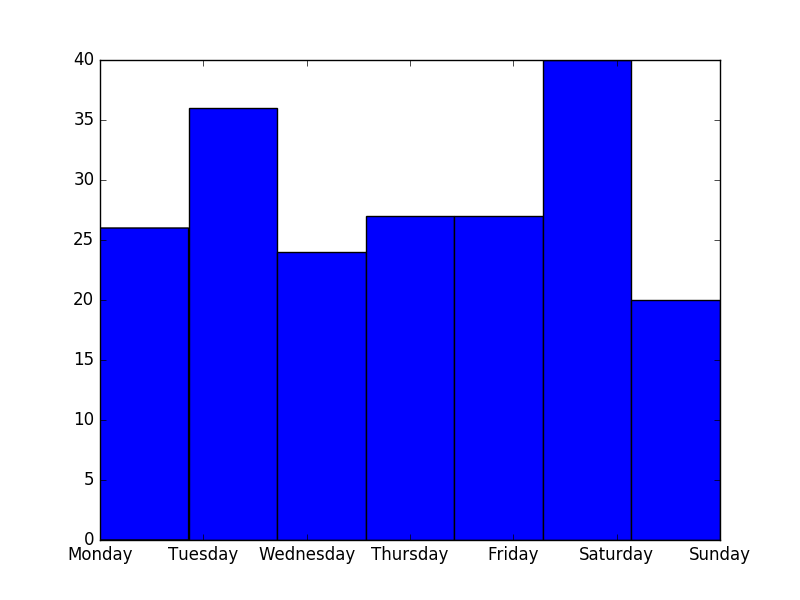
\includegraphics[width=4.16667in]{dow.png}

\subsubsection{\texorpdfstring{More \emph{DataFrame} Manipulation and
Plotting}{More DataFrame Manipulation and Plotting}}\label{more-dataframe-manipulation-and-plotting}

\texttt{DataFrame}s and \texttt{numpy} give us other ways to manipulate
data. For example, we can plot a histogram of the ages of violators like
this:

\begin{lstlisting}
>>> ages = data['Cited Person Age'].astype(int)
>>> fig = plt.figure()
>>> ax = fig.add_subplot(1, 1, 1)
>>> plt.hist(ages, bins=np.max(ages) - np.min(ages))
>>> plt.show()
\end{lstlisting}

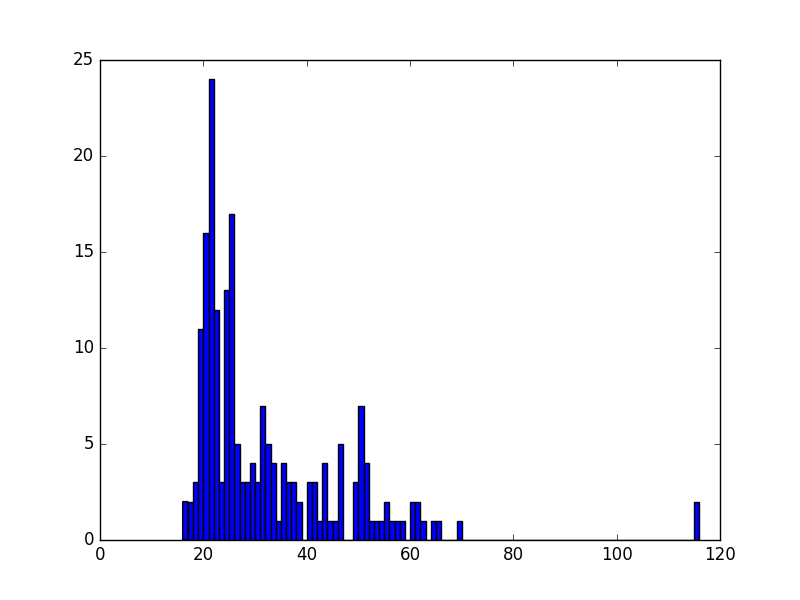
\includegraphics[width=4.16667in]{ages.png}

Surprisingly, we see some 116 year-old violators! This is probably an
error in the data, so we can remove these data points easily and plot
the histogram again:

\begin{lstlisting}
>>> ages = ages[ages < 100]
>>> fig = plt.figure()
>>> ax = fig.add_subplot(1, 1, 1)
>>> plt.hist(ages, bins=np.max(ages) - np.min(ages))
>>> plt.show()
\end{lstlisting}

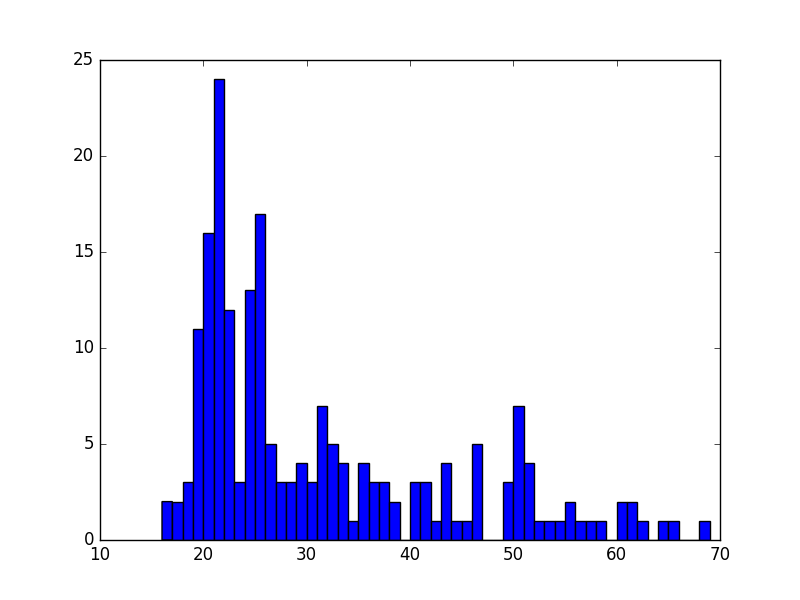
\includegraphics[width=4.16667in]{ages-filtered.png}

\subsubsection{Saving Plots to PDF}\label{saving-plots-to-pdf}

Oftentimes, you will want to save your \texttt{matplotlib} graph as a
PDF or an SVG file instead of just viewing it on your screen. For both,
we need to create a \texttt{figure} and plot the histogram as before:

\begin{lstlisting}
>>> fig = plt.figure()
>>> ax = fig.add_subplot(1, 1, 1)
>>> plt.hist(ages, bins=np.max(ages) - np.min(ages))
\end{lstlisting}

Then, instead of calling \texttt{plt.show()} we can invoke
\texttt{plt.savefig()} to save as SVG:

\begin{lstlisting}
>>> plt.savefig('hist.svg')
\end{lstlisting}

If we want to save the figure as PDF instead, we need to use the
\texttt{PdfPages} module together with \texttt{savefig()}:

\begin{lstlisting}
>>> import matplotlib.patches as mpatches
>>> from matplotlib.backends.backend_pdf import PdfPages   
>>> pp = PdfPages('hist.pdf')
>>> fig.savefig(pp, format='pdf')
>>> pp.close()
\end{lstlisting}

\subsubsection{Next Steps and Exercises}\label{next-steps-and-exercises}

There is a lot more to working with \texttt{pandas}, \texttt{numpy} and
\texttt{matplotlib} than we can show you here, but hopefully this
example has piqued your curiosity.

Don't worry if you don't understand everything in this example. For a
more detailed explanation on these modules and the examples we did,
please take a look at the tutorials below. The \texttt{numpy} and
\texttt{pandas} tutorials are mandatory if you want to be able to use
these modules, and the \texttt{matplotlib} gallery has many useful code
examples.

\subsection{Summary of Useful
Libraries}\label{summary-of-useful-libraries}

\subsubsection{Numpy}\label{numpy}

  \URL{http://www.numpy.org/}


According to the Numpy Web page "NumPy is a package for scientific
computing with Python. It contains a powerful N-dimensional array
object, sophisticated (broadcasting) functions, tools for integrating
C/C++ and Fortran code, useful linear algebra, Fourier transform, and
random number capabilities

Tutorial:
\url{https://docs.scipy.org/doc/numpy-dev/user/quickstart.html}

\subsubsection{MatplotLib}\label{matplotlib}

  \URL{http://matplotlib.org/}

According the the Matplotlib Web page, ``matplotlib is a python 2D
plotting library which produces publication quality figures in a variety
of hardcopy formats and interactive environments across platforms.
matplotlib can be used in python scripts, the python and ipython shell
(ala MATLAB®* or Mathematica®†), web application servers, and six
graphical user interface toolkits.''

Matplotlib Gallery: \url{http://matplotlib.org/gallery.html}

\subsubsection{Pandas}\label{pandas}

  \URL{http://pandas.pydata.org/}

According to the Pandas Web page, ``Pandas is a library library
providing high-performance, easy-to-use data structures and data
analysis tools for the Python programming language.''

In addition to access to charts via matplotlib it has elementary
functionality for conduction data analysis. Pandas may be very suitable
for your projects.

Tutorial: \url{http://pandas.pydata.org/pandas-docs/stable/10min.html}

Pandas Cheat Sheet:
\url{https://github.com/pandas-dev/pandas/blob/master/doc/cheatsheet/Pandas_Cheat_Sheet.pdf}

\subsection{Big Data Libraries}\label{other-useful-libraries}

\subsubsection{Scipy}\label{scipy}

  \URL{https://www.scipy.org/}

According to the SciPy Web page, ``SciPy (pronounced ``Sigh Pie'') is a
Python-based ecosystem of open-source software for mathematics, science,
and engineering. In particular, these are some of the core packages:

\begin{itemize}
\item NumPy
\item IPython
\item Pandas
\item Matplotlib
\item Sympy
\item SciPy library
\end{itemize}

It is thus an agglomeration of useful pacakes and will prbably sufice
for your projects in case you use Python.

\subsubsection{ggplot}\label{ggplot}

  \URL{http://ggplot.yhathq.com/}


According to the ggplot python Web page ggplot is a plotting system for
Python based on R's ggplot2. It allows to quickly generate some plots
quickly with little effort. Often it may be easier to use than
matplotlib directly.

\subsubsection{seaborn}\label{seaborn}

\URL{http://www.data-analysis-in-python.org/t_seaborn.html}

The good library for plotting is called seaborn which is build on top of
matplotlib. It provides high level templates for common statistical
plots.

\begin{itemize}
\item
  Gallery:
  \url{http://stanford.edu/~mwaskom/software/seaborn/examples/index.html}
\item
  Original Tutorial:
  \url{http://stanford.edu/~mwaskom/software/seaborn/tutorial.html}
\item
  Additional Tutorial:
  \url{https://stanford.edu/~mwaskom/software/seaborn/tutorial/distributions.html}
\end{itemize}

Here are some examples from a previous class:

\URL{https://github.com/bigdata-i523/hid231/blob/master/experiment/seaborn/seaborn-exercises.ipynb}
\URL{https://github.com/bigdata-i523/hid231/blob/master/experiment/learning-jupyter/learning_jupyter_notebook.ipynb}

\begin{exercise}\label{E:ipynb-export}
Take these examples and cretae sections in latex that can be added to
the book. Describe the process. 

1. export the ipynb as rst
2. use pandoc to export it to tex
3. do some cleanup on the tex files

Can this be automated with a cmd5 script such as
\begin{lstlisting}{bash}
cms ipynb [url=URL | file=FILE] --output FILENAME
\end{lstlisting}
\end{exercise}

\subsubsection{Bokeh}\label{bokeh}

Bokeh is an interactive visualization library with focus on web browsers
for display. Its goal is to provide a similar experience as D3.js

\begin{itemize}
\item
  URL: \url{http://bokeh.pydata.org/}
\item
  Gallery: \url{http://bokeh.pydata.org/en/latest/docs/gallery.html}
\end{itemize}

\subsubsection{pygal}\label{pygal}

Pygal is a simple API to produce graphs that can be easily embedded into
your Web pages. It contains annotations when you hover over data points.
It also allows to present the data in a table.

\URL{http://pygal.org/}


\subsubsection{Network and Graphs}\label{network-and-graphs}

\begin{itemize}
\tightlist
\item
  igraph: \url{http://www.pythonforsocialscientists.org/t_igraph.html}
\item
  networkx: \url{https://networkx.github.io/}
\end{itemize}

\subsubsection{REST}\label{rest}

\begin{itemize}
\tightlist
\item
  django REST FRamework \url{http://www.django-rest-framework.org/}
\item
  flask
  \url{https://blog.miguelgrinberg.com/post/designing-a-restful-api-with-python-and-flask}
\item
  requests
  \url{https://realpython.com/blog/python/api-integration-in-python/}
\item
  urllib2
  \url{http://rest.elkstein.org/2008/02/using-rest-in-python.html} (not
  recommended)
\item
  web
  \url{http://www.dreamsyssoft.com/python-scripting-tutorial/create-simple-rest-web-service-with-python.php}
  (not recommended)
\item
  bottle \url{http://bottlepy.org/docs/dev/index.html}
\item
  falcon \url{https://falconframework.org/}
\item
  eve \url{http://python-eve.org/}
\item
  \url{https://code.tutsplus.com/tutorials/building-rest-apis-using-eve--cms-22961}
\end{itemize}

\section{Parsing Data}

Being able to parse data is an important activity in the data analysis
process. Not all data may be following aspecific format and the data
may need to be extracted.


\subsection{notebook.md Parser}

We are using a notebook.md to communicate what students have done
throughout the semester. We like to make a simble cmd5 command that
parses the notebook.md file and check it upon correctness.

An example for a notebook.md file is lokated here 

\URL{https://raw.githubusercontent.com/bigdata-i523/sample-hid000/master/notebook.md}

The following code may inspire you

\URL{https://github.com/bigdata-i523/hid203/tree/master/experiment}

We like to implement the follwoing functionality and use docopts to
document the command.

\begin{lstlisting}
cms class notebook [--git=GITREPONAME] --verify hid

    verifies the correctness of the notebook.md file

cms class notebook [--git=GITREPONAME] --log

    displays the log of the notebook.md

cms class notebook [--git=GITREPONAME] --history

    displays a true or false for each week since the first occurance
    of the notebook.md file in the git repository
\end{lstlisting}

\begin{exercise}
  \label{E:notebook-md.1}
  Write a notebook.md parser
\end{exercise}

\begin{exercise}
  \label{E:notebook-md.2}
  How can this command be generalized to provide not only information
  for a student but to provide information for the class. Example: can
  we identify prefered days of when the notebooks are checked in. Can
  we identify a list of students that have not updated the notebok for
  a week?  Can we identify the list of student s that have updated the
  notebook for a week? 
\end{exercise}


\subsection{Video Length}

The Latex source of this class contains a macro to include videos.


Given a LateX file, can you create a table that includes the names of
all videos in that file and sums up the total viewing time. Previously
the document was stored in RST and the code from a previous student
may inspire you. Can you reqrite it in for LaTeX? 

\URL{https://github.com/bigdata-i523/hid107/blob/master/cloudmesh/bar/command/mycommand.py}


\begin{lstlisting}
cms class video list FILENAME --output=[tabular|longtable|csv|txt]

    prints the videolist in the given format. txt means it is just ASCII
\end{lstlisting}

\begin{comment}
The previous work even summarized the video length by chapter.

see: https://piazza.com/class/j5wll7vzylg25j?cid=325
\end{comment}

\begin{exercise}
Write a tool that extracts the information for video length. 
\end{exercise}

\begin{exercise}
Write a tool that finds all youtube urls that are not in a video latex
macro.
\end{exercise}

\subsection{Dask}
\index{Dask}

Many times operations need to be done on data in parallel to utilize
modern processor architectures.


Dask provides a \textit{dynamic task scheduling} which is optimized for
computation. It is similar to other frameworks such as Airflow, Luigi,
Celery, or Make. HOwever it is specializing in optimized interactive
computational workloads.

Furthermore, Dask targets Big Data \textit{collections} such as parallel
arrays, dataframes, and lists. Thes ecollections ar commonly found in
NumPy, Pandas, or Python iterators to larger-than-memory or
distributed environments. While using the Dask implementation we can
replace the original imports from the appropriate framework, replace
them with Dask imports and implicity use parallel collections that
utilize internally the dynamic task schedulers.

More information can be found at:

\URL{https://dask.pydata.org}

\begin{exercise}
Conduct a preformance study that showcases the difference of doing
parallel calculations in Dask, claculations in a framework such as
SciPy, and regular unthreaded python code.
\end{exercise}



\FILENAME\
\section{cmd Module}\label{cmd-module}
\index{cmd}

\subsection{Introduction}\label{introduction}

The Python cmd module is useful for any more involved command-line
application. It is used in the
\href{http://cloudmesh.github.io/}{Cloudmesh Project}, for example, and
students in I524
\textless{}../../i524/index\textgreater{} have found it helpful in their
projects. The Python cmd module contains a public class, Cmd, designed
to be used as a base class for command processors such as interactive
shells and other command interpreters.

\subsection{\texorpdfstring{\emph{Hello, World} with
cmd}{Hello, World with cmd}}\label{hello-world-with-cmd}

This example shows a very simple command interpreter that simply
responds to the greet command.

In order to demonstrate commands provided by cmd, let's save the
following program in a file called helloworld.py.

\begin{lstlisting}
from __future__ import print_function, division
import cmd


class HelloWorld(cmd.Cmd):
    '''Simple command processor example.'''

    def do_greet(self, line):
        if line is not None and len(line.strip()) > 0:
            print('Hello, %s!' % line.strip().title())
        else:
            print('Hello!')

    def do_EOF(self, line):
        print('bye, bye')
        return True


if __name__ == '__main__':
    HelloWorld().cmdloop()
\end{lstlisting}

A session with this program might look like this:

\begin{lstlisting}
$ python helloworld.py

(Cmd) help

Documented commands (type help <topic>):
========================================
help

Undocumented commands:
======================
EOF  greet

(Cmd) greet
Hello!
(Cmd) greet albert
Hello, Albert!
<CTRL-D pressed>
(Cmd) bye, bye
\end{lstlisting}

The Cmd class can be used to customize a subclass that becomes a
user-defined command prompt. After you have executed your program,
commands defined in your class can be used. Take note of the following
in this example:

\begin{itemize}

\item
  The methods of the class of the form do\_xxx implement the shell
  commands, with xxx being the name of the command. For example, in the
  HelloWorld class, the function do\_greet maps to the greet on the
  command line.
\item
  The EOF command is a special command that is executed when you press
  CTRL-D on your keyboard.
\item
  As soon as any command method returns True the shell application
  exits. Thus, in this example the shell is exited by pressing CTRL-D,
  since the do\_EOF method is the only one that returns True.
\item
  The shell application is started by calling the cmdloop method of the
  class.
\end{itemize}

\subsection{A More Involved Example}\label{a-more-involved-example}

Let's look at a little more involved example. Save the following code in
a file called calculator.py.

\begin{lstlisting}
from __future__ import print_function, division
import cmd


class Calculator(cmd.Cmd):
 prompt = 'calc >>> '
 intro = 'Simple calculator that can do addition, subtraction, multiplication and division.'

 def do_add(self, line):
     args = line.split()
     total = 0
     for arg in args:
         total += float(arg.strip())
     print(total)

 def do_subtract(self, line):
     args = line.split()
     total = 0
     if len(args) > 0:
         total = float(args[0])
     for arg in args[1:]:
         total -= float(arg.strip())
     print(total)

 def do_EOF(self, line):
     print('bye, bye')
     return True


if __name__ == '__main__':
 Calculator().cmdloop()
\end{lstlisting}

A session with this program might look like this:

\begin{lstlisting}
$ python calculator.py
Simple calculator that can do addition, subtraction, multiplication and division.
calc >>> help

Documented commands (type help <topic>):
========================================
help

Undocumented commands:
======================
EOF  add  subtract

calc >>> add
0
calc >>> add 4 5 6
15.0
calc >>> subtract
0
calc >>> subtract 10 2
8.0
calc >>> subtract 10 2 20
-12.0
calc >>> bye, bye
\end{lstlisting}

\begin{itemize}

\item
  In this case we are using the prompt and intro class variables to
  define what the default prompt looks like and a welcome message when
  the command interpreter is invoked.
\item
  In the add and subtract commands we are using the strip and split
  methods to parse all arguments. If you want to get fancy, you can use
  Python modules like getopts or argparse for this, but this is not
  necessary in this simple example.
\end{itemize}

\subsection{Help Messages}\label{help-messages}

Notice that all commands presently show up as undocumented. To remedy
this, we can define help\_ methods for each command:

\begin{lstlisting}
from __future__ import print_function, division
import cmd


class Calculator(cmd.Cmd):
  prompt = 'calc >>> '
  intro = 'Simple calculator that can do addition, subtraction, multiplication and division.'

  def do_add(self, line):
      args = line.split()
      total = 0
      for arg in args:
          total += float(arg.strip())
      print(total)

  def help_add(self):
      print('\n'.join([
          'add [number,]',
          'Add the arguments together and display the total.'
      ]))

  def do_subtract(self, line):
      args = line.split()
      total = 0
      if len(args) > 0:
          total = float(args[0])
      for arg in args[1:]:
          total -= float(arg.strip())
      print(total)

  def help_subtract(self):
      print('\n'.join([
          'subtract [number,]',
          'Subtract all following arguments from the first argument.'
      ]))

  def do_EOF(self, line):
      print('bye, bye')
      return True


if __name__ == '__main__':
  Calculator().cmdloop()
\end{lstlisting}

Now, we can obtain help for the add and subtract commands:

\begin{lstlisting}
$ python calculator.py
Simple calculator that can do addition, subtraction, multiplication and division.
calc >>> help

Documented commands (type help <topic>):
========================================
add  help  subtract

Undocumented commands:
======================
EOF

calc >>> help add
add [number,]
Add the arguments together and display the total.
calc >>> help subtract
subtract [number,]
Subtract all following arguments from the first argument.
calc >>> bye, bye
\end{lstlisting}
%$

\subsection{Useful Links}\label{useful-links}

\begin{itemize}

\item
  \href{https://docs.python.org/2/library/cmd.html}{Python Docs}
\item
  \href{https://pymotw.com/2/cmd/}{Python Module of the Week: cmd --
  Create line-oriented command processors}
\end{itemize}

\section{Word Count with Parallel Python}\label{word-count-1-parallel-python}

\subsection{Introduction}

In this lesson we will demonstrate Python's \texttt{multiprocessing} API
for parallel computation by writing a program that counts how many times
each word in a collection of documents appear.

\subsection{Generating a Document Collection}

Before we begin, let's write a script that will let us generate document
collections by specifying the number of documents and the number of
words per document. This will make benchmarking later straightforward.

To keep it simple, the vocabulary of the document collection will
consist of random numbers rather than the words of an actual language:

\begin{lstlisting}
'''Usage: generate_nums.py [-h] NUM_LISTS INTS_PER_LIST MIN_INT MAX_INT DEST_DIR

Generate random lists of integers and save them as 1.txt, 2.txt, etc.

Arguments:
   NUM_LISTS     The number of lists to create.
   INTS_PER_LIST The number of integers in each list.
   MIN_NUM       Each generated integer will be >= MIN_NUM.
   MAX_NUM       Each generated integer will be <= MAX_NUM.
   DEST_DIR      A directory where the generated numbers will be stored.

Options:
  -h --help
'''

from __future__ import print_function
import os, random, logging
from docopt import docopt


def generate_random_lists(num_lists, ints_per_list, min_int, max_int):
   return [[random.randint(min_int, max_int) for _ in range(ints_per_list)] for _ in range(num_lists)]


if __name__ == '__main__':
   args = docopt(__doc__)
   num_lists, ints_per_list, min_int, max_int, dest_dir = [
      int(args['NUM_LISTS']),
  int(args['INTS_PER_LIST']),
  int(args['MIN_INT']),
  int(args['MAX_INT']),
  args['DEST_DIR']
   ]

   if not os.path.exists(dest_dir):
      os.makedirs(dest_dir)

   lists = generate_random_lists(num_lists, ints_per_list, min_int, max_int)
   curr_list = 1
   for lst in lists:
      with open(os.path.join(dest_dir, '%d.txt' % curr_list), 'w') as f:
     f.write(os.linesep.join(map(str, lst)))
  curr_list += 1
   logging.debug('Numbers written.')
\end{lstlisting}

Notice that we are using the
\href{https://pypi.python.org/pypi/docopt}{docopt} module that you
should be familiar with from the
Intro to Python \textless{}python\_intro\textgreater{} tutorial to make
the script easy to run from the command line.

You can generate a document collection with this script as follows:

\begin{lstlisting}
python generate_nums.py 1000 10000 0 100 docs-1000-10000
\end{lstlisting}

\subsection{Serial Implementation}

A first serial implementation of wordcount is straightforward:

\begin{lstlisting}
'''Usage: wordcount.py [-h] DATA_DIR

Read a collection of .txt documents and count how many times each word
appears in the collection.  

Arguments:
  DATA_DIR  A directory with documents (.txt files).

Options:
  -h --help
'''

from __future__ import division, print_function
import os, glob, logging
from docopt import docopt

logging.basicConfig(level=logging.DEBUG)


def wordcount(files):
   counts = {}
   for filepath in files:
      with open(filepath, 'r') as f:
     words = [word.strip() for word in f.read().split()]
     for word in words:
        if word not in counts:
           counts[word] = 0
        counts[word] += 1
   return counts


if __name__ == '__main__':
   args = docopt(__doc__)
   if not os.path.exists(args['DATA_DIR']):
      raise ValueError('Invalid data directory: %s' % args['DATA_DIR'])

   counts = wordcount(glob.glob(os.path.join(args['DATA_DIR'], '*.txt')))
   logging.debug(counts)
\end{lstlisting}

\subsection{Serial Implementation Using map and reduce}

We can improve the serial plementation in anticipation of parallelizing
the program by making use of Python's \texttt{map} and \texttt{reduce}
functions.

In short, you can use \texttt{map} to apply the same function to the
members of a collection. For example, to convert a list of numbers to
strings, you could do:

\begin{lstlisting}
import random
nums = [random.randint(1, 2) for _ in range(10)]
print(nums)
[2, 1, 1, 1, 2, 2, 2, 2, 2, 2]
print(map(str, nums))
['2', '1', '1', '1', '2', '2', '2', '2', '2', '2']
\end{lstlisting}

We can use reduce to apply the same function cumulatively to the items
of a sequence. For example, to find the total of the numbers in our
list, we could use \texttt{reduce} as follows:

\begin{lstlisting}
def add(x, y): 
    return x + y

print(reduce(add, nums))
17
\end{lstlisting}

We can simplify this even more by using a lambda function:

\begin{lstlisting}
print(reduce(lambda x, y: x + y, nums))
17
\end{lstlisting}

You can read more about
\href{https://docs.python.org/2.7/tutorial/controlflow.html\#lambda-expressions}{Python's
lambda function in the docs}.

With this in mind, we can reimplement the wordcount example as follows:

\begin{lstlisting}
'''Usage: wordcount_mapreduce.py [-h] DATA_DIR

Read a collection of .txt documents and count how many times each word
appears in the collection.  

Arguments: 
   DATA_DIR  A directory with documents (.txt files).

Options:
   -h --help
'''

from __future__ import division, print_function
import os, glob, logging
from docopt import docopt

logging.basicConfig(level=logging.DEBUG)

def count_words(filepath):
   counts = {}
   with open(filepath, 'r') as f:
      words = [word.strip() for word in f.read().split()]

  for word in words:
     if word not in counts:
        counts[word] = 0
     counts[word] += 1
  return counts


def merge_counts(counts1, counts2):
   for word, count in counts2.items():
      if word not in counts1:
     counts1[word] = 0
  counts1[word] += counts2[word]
   return counts1


if __name__ == '__main__':
   args = docopt(__doc__)
   if not os.path.exists(args['DATA_DIR']):
      raise ValueError('Invalid data directory: %s' % args['DATA_DIR'])

   per_doc_counts = map(count_words, glob.glob(os.path.join(args['DATA_DIR'], '*.txt')))
   counts = reduce(merge_counts, [{}] + per_doc_counts)
   logging.debug(counts)
\end{lstlisting}

\subsection{Parallel Implementation}

Drawing on the previous implementation using \texttt{map} and
\texttt{reduce}, we can parallelize the implementation using Python's
\texttt{multiprocessing} API:

\begin{lstlisting}
'''Usage: wordcount_mapreduce_parallel.py [-h] DATA_DIR NUM_PROCESSES

Read a collection of .txt documents and count, in parallel, how many
times each word appears in the collection.

Arguments:
   DATA_DIR       A directory with documents (.txt files).
   NUM_PROCESSES  The number of parallel processes to use.

Options:
   -h --help
'''

from __future__ import division, print_function
import os, glob, logging
from docopt import docopt
from wordcount_mapreduce import count_words, merge_counts
from multiprocessing import Pool

logging.basicConfig(level=logging.DEBUG)

if __name__ == '__main__':
   args = docopt(__doc__)
   if not os.path.exists(args['DATA_DIR']):
      raise ValueError('Invalid data directory: %s' % args['DATA_DIR'])
   num_processes = int(args['NUM_PROCESSES'])

   pool = Pool(processes=num_processes)
   per_doc_counts = pool.map(count_words, glob.glob(os.path.join(args['DATA_DIR'], '*.txt')))
   counts = reduce(merge_counts, [{}] + per_doc_counts)
   logging.debug(counts)
\end{lstlisting}

\subsection{Questions}

To time each of the examples above, enter it into its own Python file
and use Linux's \texttt{time} command:


\begin{lstlisting}{language=bash}
$ time python wordcount.py docs-1000-10000
\end{lstlisting}

The output contains the real run time and the user run time. real is
wall clock time - time from start to finish of the call. user is the
amount of CPU time spent in user-mode code (outside the kernel) within
the process, that is, only actual CPU time used in executing the
process.

Run the three different programs (serial, seria w/ map and reduce,
parallel) and answer the following questions:

\begin{enumerate}
\item Is there any performance difference between the different
  versions of the program?
\item
  Does user time significantly differ from real time for any of the
  versions of the program?
\item
  Experiment with different numbers of processes for the parallel
  example, starting with 1. What is the performance gain when you goal
  from 1 to 2 processes? From 2 to 3? When do you stop seeing
  improvement? (this will depend on your machine architecture)
\end{enumerate}

\subsection{Next Steps}\label{next-steps}

In the next tutorials in this series, we will implement the
\texttt{wordcount} example in Hadoop, Pig, and will deploy it to
Chameleon Cloud.

\subsection{Useful Links}\label{useful-links}

\href{http://book.pythontips.com/en/latest/map_filter.html}{Map, Filter
and Reduce}
\href{https://docs.python.org/2/library/multiprocessing.html}{multiprocessing
API}

/FILENAME/
\section{Ubuntu Development Configurations}

\subsection{Development Configuration}

The documentation on how to configure the virtual machine and install many useful programs is posted at:

\URL{https://github.com/cloudmesh/ansible-cloudmesh-ubuntu-xenial}

You simply have to execute the following commands in the terminal of the virtual machine. In order to eliminate confusion with other terminals, we use the prefix 
\begin{verbatim}
vm> $ 
\end{verbatim}

to indicate any command that is to be started on the virtual machine. Otherwise it is clear from the context:

\begin{lstlisting}
vm>$ wget https://raw.githubusercontent.com/cloudmesh/ansible-cloudmesh-ubuntu-xenial/master/bootstrap.sh
vm>$ bash bootstrap.sh
\end{lstlisting} 

A video showcasing this install is available:

Video: 
\URL{https://youtu.be/YqXIj_Wzfsc}

A video showcasing the upload to gitlab from within the vm using commandline tools

Video: 
\URL{https://youtu.be/EnpneUY82I8}

\section{Refcards}\label{refcards}
\index{Refcards}
\index{Refcards!emacs}
\index{Refcards!vi}
\index{Refcards!Makefile}
\index{Refcards!R}
\index{Refcards!Python}
\index{Refcards!Python!Data}
\index{Refcards!LaTeX}
\index{Refcards!vim}
\index{Refcards!git}
\index{Refcards!rst}
\index{Refcards!OpenStack}

\FILENAME\


We present you with a list of useful short refrence cards. This cards
can be extremly useful to remind yourself about some important commands
and features. Having them could simplify your interaction with the
systems, We not only collected here some refcards about Linux, but also
about other useful tools and services.

If you like to add new topics, let us know via your contribution (see
the contribution section).
{\footnotesize
\begin{longtable}{p{2.5cm}p{11.5cm}}
\toprule
Emacs
 & 
\url{https://www.gnu.org/software/emacs/refcards/pdf/refcard.pdf}
\tabularnewline
Vi
 & 
\url{http://www.ks.uiuc.edu/Training/Tutorials/Reference/virefcard.pdf}
\tabularnewline
Linux
 & 
\url{http://www.cs.jhu.edu/~joanne/unixRC.pdf}
\tabularnewline
Makefile
 & 
\url{http://www.tofgarion.net/lectures/IN323/refcards/refcardMakeIN323.pdf}
\tabularnewline
R
 & 
\url{https://cran.r-project.org/doc/contrib/Short-refcard.pdf}
\tabularnewline
Python
 & 
\url{https://dzone.com/refcardz/core-python}
\tabularnewline
Python Data
 & 
\url{https://dzone.com/refcardz/data-mining-discovering-and}
\tabularnewline
SQL
 & 
\url{http://www.digilife.be/quickreferences/QRC/MySQL-4.02a.pdf}
\tabularnewline
Vim
 & 
\url{http://michaelgoerz.net/refcards/vimqrc.pdf}
\tabularnewline
LaTeX
 & 
\url{https://wch.github.io/latexsheet/latexsheet.pdf}
\tabularnewline
Git
 & 
\url{https://education.github.com/git-cheat-sheet-education.pdf}
\tabularnewline
Openstack
 & 
\url{http://docs.openstack.org/user-guide/cli_cheat_sheet.html}
\tabularnewline
Openstack
 & 
\url{http://cmias.free.fr/IMG/pdf/rc208_010d-openstack_2.pdf}
\tabularnewline
RST
 & 
\url{https://github.com/ralsina/rst-cheatsheet/blob/master/rst-cheatsheet.pdf}
\tabularnewline
\bottomrule
\end{longtable}
}

Others:
{\footnotesize
\begin{longtable}{p{2.5cm}p{11.5cm}}
\toprule
  Numpi/Pandas &
  \url{http://www.cheat-sheets.org/saved-copy/NumPy_SciPy_Pandas_Quandl_Cheat_Sheet.pdf}
\tabularnewline
  Cheat Sheets & \url{http://www.cheat-sheets.org/}
\tabularnewline
  Python Tutorial &
  \url{http://fivedots.coe.psu.ac.th/Software.coe/learnPython/Cheat\%20Sheets/python2.pdf}
\tabularnewline
  Python &
  \url{http://www.cheat-sheets.org/saved-copy/PQRC-2.4-A4-latest.pdf}
\tabularnewline
  Python &
  \url{https://www.cheatography.com/davechild/cheat-sheets/python/pdf/}
\tabularnewline
  Python API Index & \url{http://overapi.com/python}
\tabularnewline
  Python 3 &
  \url{https://perso.limsi.fr/pointal/_media/python:cours:mementopython3-english.pdf}
\tabularnewline
\bottomrule
\end{longtable}

\section{Datasets}\label{datasets}
\index{Datasets}
/FILENAME/

Below are links to collections of datasets that may be of use for
homework assignments or projects.

\begin{itemize}

\item
  \url{https://www.data.gov/}
\item
  \url{https://github.com/caesar0301/awesome-public-datasets}
\item
  \url{https://aws.amazon.com/public-data-sets/}
\item
  \url{https://www.kaggle.com/datasets}
\item
  \url{https://cloud.google.com/bigquery/public-data/github}
\item
  \url{https://www.quora.com/Where-can-I-find-large-datasets-open-to-the-public}
\end{itemize}

For NIST Projects:

\begin{itemize}

\item
  \href{http://www.nist.gov/itl/iad/ig/sd27a.cfm}{NIST Special Database
  27A - 4GB}
\item
  \href{http://pascal.inrialpes.fr/data/human/}{INRIA Person Dataset}
\item
  \href{https://www.cms.gov/Research-Statistics-Data-and-Systems/Downloadable-Public-Use-Files/Part-B-National-Summary-Data-File/Overview.html}{Healthcare
  data from CMS}
\item
  \href{https://github.com/fivethirtyeight/uber-tlc-foil-response}{Uber
  Ride Sharing GPS Data}
\item
  \href{http://www.census.gov/population/www/cen2010/glance/}{Census
  Data}
\end{itemize}

\section{Ansible I: Simplest Example}\label{ansible-i-simplest-example}

/FILENAME/

\subsection{Prerequisite}\label{prerequisite}

In order to conduct this lesson:

\begin{itemize}
\item
  You can install Ubuntu 16.04 virtual machine on VirtualBox
\item
  You can install software packages via `apt-get' tool in Ubuntu virtual
  host
\item
  You already reserved a virtual cluster (with at least 1 virtual
  machine in it) on some cloud. OR you can use VMs installed in
  VirtualBox instead.
\item
  You set up SSH credentials and can login to your virtual machines.
\end{itemize}

\subsection{What can you do with
Ansible?}\label{what-can-you-do-with-ansible}

Humans do maintenance and configurations on computers. Essentially, we
specify a list of operations and a list of target machines where the
operations apply to. After defining these two critical lists, the
creative works are done, and the rest labour can be automated. And this
is what Ansible is used for.

Let us develop a sample from scratch, based on this paradigm.

\subsection{A sample use case}\label{a-sample-use-case}

In this example, we are going to use Ansible to install Apache server on
our VMs.

\begin{itemize}

\item
  install Ansible tool on your machine first
\end{itemize}

\begin{lstlisting}
$ sudo apt-get update
$ sudo apt-get install ansible
\end{lstlisting}

\begin{itemize}

\item
  prepare a working environment for your Ansible
\end{itemize}

\begin{lstlisting}
$ mkdir}ansible-apache
$ cd ansible-apache
\end{lstlisting}

\begin{itemize}

\item
  next, we are going to create a local configuration file for Ansible.
\end{itemize}

When you execute Ansible within this folder, this local configuration
file is always going to overwrite a system level Ansible configuration.
It is in general beneficial to keep custom configurations locally unless
you absolutely believe it should be applied system wide. Create a file
`ansible.cfg' in this folder, and fill:

\begin{verbatim}
[defaults]
hostfile = hosts
\end{verbatim}

This local configuration file simple tells that the target machines'
names are given in a file named `hosts'

In your assignments, we choose to use \texttt{inventory} instead of
\texttt{ansible.cfg}. More details will be given when we introduce
\texttt{ansible-galaxy} in following chapters. At this moment, getting
yourself familiar with some concepts of configuring the Ansible
environment is good enough.

\begin{itemize}

\item
  specify hosts in the file
\end{itemize}

You should have accesses to all VMs listed in this file as part of our
prerequisites. Create and edit file `hosts':

\begin{verbatim}
[apache]
<server_ip> ansible_ssh_user=<server_username>
\end{verbatim}

The name `apache' in the brackets defines the server group name. We will
use this name to refer to all server items in this group next. Fill in
IP addresses of the virtual machines you launched in your VirtualBox and
fire up these VMs in you VirtualBox.

\begin{itemize}

\item
  compose a playbook
\end{itemize}

A playbook tells Ansible what to do. it uses YAML Markup syntax. Create
and edit a file with a proper name e.g. apache.yml as follow:

\begin{verbatim}
---
- hosts: apache #comment: apache is the group name we just defined
  become: yes #comment: this operation needs privilege access
  tasks:
    - name: install apache2 # text description
      apt: name=apache2 update_cache=yes state=latest
\end{verbatim}

This block defines the target VMs and operations(tasks) need to apply.
you may wonder what `apt' means. here comes the concept of Ansible
modules in next paragraph.

\subsection{The concept of modules}\label{the-concept-of-modules}

`apt' is the module used in our sample playbook. it installs packages on
Ubuntu for us.

Ansible relies on various kinds of modules to fulfil tasks on the remote
servers. These modules are developed for particular tasks and take in
related arguments. For instance, when we use `apt' module, we certainly
need to tell which package we intend to install. That is why we provide
a value for the `name' argument.

\subsection{Run you playbook}\label{run-you-playbook}

In the same folder, execute

\begin{lstlisting}
ansible-playbook apache.yml --ask-sudo-pass
\end{lstlisting}

After a successful run, open a browser and fill in your server IP. you
should se a `It works!' Apache2 Ubuntu default page. Make sure the
security policy on your cloud opens port 80 to let the HTTP traffic go
through.

Ansible playbook can have more complex and fancy structure and syntaxes.
Go explore! this sample is based on:
\url{https://www.digitalocean.com/community/tutorials/how-to-configure-apache-using-ansible-on-ubuntu-14-04}

We are going to offer an advanced Ansible in next chapter.
\section{Ansible II: Roles}\label{ansible-ii-roles}

In this example, we are going to install R package onto your cloud VMs.
R is a useful statistic programing language commonly used in many
scientific and statistics computing projects, maybe also the one you
chose for this class.

In addition to last basic example, we are going to illustrate the
concept of Ansible Roles, install source code through Github, and make
use of variables. These are key features you will find useful in your
project deployments.

We are going to use a top-down fashion in this example. We first start
from a playbook that is already good to go. You can execute this
playbook (don't do it yet) to get R installed in your remote hosts. We
then further complicate this concise playbook by introducing
functionalities to do the same tasks but in different ways. Although
these detours are not necessary in this simply case, it helps you grasp
the power of Ansible and ease your life when they are needed in your
real projects.

\subsection{Prerequisite}\label{prerequisite}

\begin{itemize}

\item
  Finished Ansible Lesson I
\item
  Have VMs reserved on cloud and SSH Key setup
\end{itemize}

\subsection{A completed playbook}\label{a-completed-playbook}

From the earlier example, we already can compose a playbook
`example.yml' that install a software package, for example:

\begin{verbatim}
---
- hosts: R_hosts
  become: yes
  tasks:
    - name: install the R package
      apt: name=r-base update_cache=yes state=latest
\end{verbatim}

the hosts are defined in a file `hosts', which we configured in
`ansible.cfg':

\begin{verbatim}
[R_hosts]
<cloud_server_ip> ansible_ssh_user=<cloud_server_username>
\end{verbatim}

In your assignments, we choose to use \texttt{inventory} instead of
\texttt{ansible.cfg}. More details will be given when we introduce
\texttt{ansible-galaxy} in following chapters. At this moment, getting
yourself familiar with some concepts of configuring the Ansible
environment is good enough.

This should get the installation job done. But we are going to extend it
via new features next.

\subsection{Introducing Roles}\label{introducing-roles}

Role is an important concept used very often in large Ansible projects.
You divide a series of tasks into different groups. Each group
corresponds to certain role of the whole project.

For example, if your project is to deploy a web site, you may need to
install the back end database, the web server that responses HTTP
requests and the web application itself. They are three different roles
and should carry out their own installation and configuration tasks.

Even though we only need to install the R package in this example, we
can still do it by defining a role `r'. Modify your `example.yml' to be:

\begin{verbatim}
---
- hosts: R_hosts

  roles:
    - r
\end{verbatim}

and create directory structure in your top project directory:

\begin{verbatim}
$ mkdir -p roles/r/tasks
$ touch roles/r/tasks/main.yml
\end{verbatim}

edit this `main.yml' to be:

\begin{verbatim}
---
- name: install the R package
  apt: name=r-base update_cache=yes state=latest
  become: yes
\end{verbatim}

You probably already get the point. We take the `tasks' section out of
the one-for-all example.yml and re-organize them into roles. Each role
specified in example.yml should have its own directory under roles/ and
the tasks need be done by this role is listed in a file `tasks/main.yml'
as above.

\subsection{Install source code from
Github}\label{install-source-code-from-github}

Although R can be installed through the OS package manager (apt-get
etc.), the software used in your projects may not. Many research
projects are available by Git instead. Here we are going to show you how
to install packages from their Git repositories. Instead of directly
executing the module `apt', we pretend Ubuntu does not provide this
package and you have to find it on Git. The source code of R can be
found at \url{https://github.com/wch/r-source.git}. We are going to
clone it to a remote VM's hard drive, build the package and install the
binary there.

To do so, we need a few new Ansible modules. You may remember from last
example that Ansible modules assist us to do various kinds of jobs when
fed correct arguments. No surprise, Ansible has a module `git' to take
care of git-related works, and a `command' module to run shell commands.
Let's modify `roles/r/tasks/main.yml' to be:

\begin{verbatim}
---
- name: get R package source
  git:
    repo: https://github.com/wch/r-source.git
    dest: /tmp/R

- name: build and install R
  become: yes
  command: chdir=/tmp/R "{{ item }}"
  with_items:
    - ./configure
    - make
    - make install
\end{verbatim}

The role `r' carries out its two tasks now. One to clone the R source
code into /tmp/R, the other uses a series of shell commands to build and
install the packages.

Note that the commands executed by the second task may not be available
on a fresh VM image. But the point of this example is to show an
alternative way to install packages, so we conveniently assume
conditions are all met.

\subsection{Using variables in a separate
file}\label{using-variables-in-a-separate-file}

We typed several string constants in our Ansible scripts so far. In
general, it is a good practice to give these values names and use them
by referring to their names. This way, you complex Ansible project can
be less error prone. Create a file in the same directory, and name it
`vars.yml':

\begin{verbatim}
---
repository: https://github.com/wch/r-source.git
tmp: /tmp/R
\end{verbatim}

Accordingly, we will update our `example.yml':

\begin{verbatim}
---
- hosts: R_hosts
  vars_files:
    - vars.yml
  roles:
    - r
\end{verbatim}

As shown, we specify a `vars\_files' telling the script that the file
`vars.yml' is going to supply variable values, whose keys are denoted by
Double curly brackets like in `roles/r/tasks/main.yml':

\begin{verbatim}
---
- name: get R package source
  git:
    repo: "{{ repository }}"
    dest: "{{ tmp }}"

- name: build and install R
  become: yes
  command: chdir="{{ tmp }}" "{{ item }}"
  with_items:
    - ./configure
    - make
    - make install
\end{verbatim}

\subsection{Summarize}\label{summarize}

Now, just edit the `hosts' file with your target VMs' IP addresses and
execute the playbook.

You should be able to extend the Ansible playbook for your project.
Configuration tools like Ansible are important components to master the
cloud environment. There is much to explore and it's worth it.
\section{Ansible III: Ansible Galaxy}\label{ansible-iii-ansible-galaxy}

By finishing the first two chapters, you should be able to compose
Ansible projects to install, configure or do other maintenances on your
software packages. We introduced the powerful component \texttt{Roles}
in the previous chapters, and emphasized the concepts of modularize and
re-usability. With these preparations, we are ready to start working on
Ansible Galaxy.

Think Ansible Galaxy as of an marketplace, where developers can share
Ansible Roles to complete their system administration tasks. Roles
exchanged in Ansible Galaxy community need to follow common conventions
so that all participants know what to expect. We will illustrate details
in this chapter.

It is good to follow the Ansible Galaxy standard during your development
assignment as much as possible, however, you will submit your
assignments to this class's repository not the global Galaxy community.

\subsection{Ansible Galaxy helloworld}\label{ansible-galaxy-helloworld}

Let us start with a simplest case: We will build an Ansible Galaxy
project. This project will install the Emacs software package on your
localhost as the target host. It is a ``helloworld'' project only meant
to get us familiar with Ansible Galaxy project structures.

\subsubsection{create the directory}\label{create-the-directory}

Setup your submission directory after you clone and rebased with
\url{https://github.com/cloudmesh/sp17-i524}:

\begin{verbatim}
$ git rebase upstream/master
$ ./setup galaxy <your HID>
\end{verbatim}

It will create a folder named after your HID inside directory galaxy/.
Your Galaxy related assignments will be completed and submitted there.
Go ahead and create files \texttt{README.md}, \texttt{playbook.yml},
\texttt{inventory} and a subdirectory \texttt{roles/} then. playbook.yml
is your project playbook. It should perform the Emacs installation task
by executing the corresponding role you will develop in the folder
`roles/'. The only difference is that we will construct the role with
the help of ansible-galaxy this time.

Now, let ansible-galaxy initialize the directory structure for you:

\begin{verbatim}
$ cd roles
$ ansible-galaxy init <to-be-created-role-name>
\end{verbatim}

The naming convention is to concatenate your name and the role name by a
dot. Here is how it looks like:

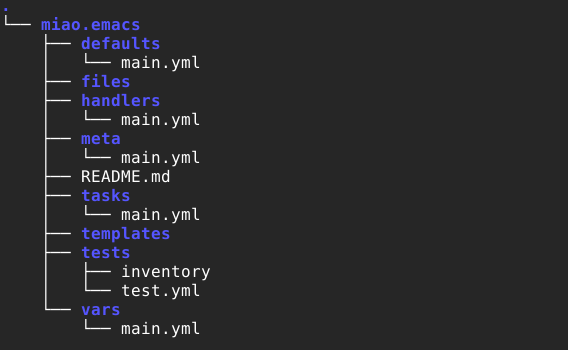
\includegraphics{/images/ansible-galaxy-init-structure.png}

\subsubsection{fill in information}\label{fill-in-information}

Let us fill in information to our project. There are several
\texttt{main.yml} files in different folders, and we will illustrate
their usages.

\begin{description}
\item[defaults and vars:]
These folders should hold variables key-value pairs for your playbook
scripts. We will leave them empty in this example.
\item[files:]
This folder is for files need to be copied to the target hosts. Data
files or configuration files can be specified if needed. We will leave
it empty too.
\item[templates:]
Similar missions to files/, templates is allocated for template files.
Keep empty for a simple Emacs installation.
\item[handlers:]
This is reserved for services running on target hosts. For example, to
restart a service under certain circumstance.
\end{description}

tasks:

\begin{quote}
This file is the actual script for all tasks. You can use the role you
built previously for Emacs installation here:

\begin{verbatim}
---
- name: install Emacs on Ubuntu 16.04
  become: yes
  package: name=emacs state=present
\end{verbatim}
\end{quote}

\begin{description}
\item[meta:]
Provide necessary metatdata for our Ansible Galaxy project for shipping:

\begin{verbatim}
---
galaxy_info:
  author: <you name>
  description: emacs installation on Ubuntu 16.04
  license:
    - MIT
  min_ansible_version: 2.0
  platforms:
    - name: Ubuntu
      versions:
        - xenial
  galaxy_tags:
    - development

dependencies: []
\end{verbatim}
\end{description}

\subsubsection{Test it out}\label{test-it-out}

You have your Ansible Galaxy role ready now. To test it as a user, go to
your HID directory and edit the other two files \texttt{inventory} and
\texttt{playbook.yml}, which are already generated for you in directory
\texttt{tests} by the script:

\begin{verbatim}
$ ansible-playbook -i ./hosts playbook.yml
\end{verbatim}

After running this playbook, you should have Emacs installed on
localhost.

\subsection{A Complete Ansible Galaxy
Project}\label{a-complete-ansible-galaxy-project}

We are going to use ansible-galaxy to setup a sample project. This
sample project will:

\begin{itemize}

\item
  use a cloud cluster with multiple VMs
\item
  deploy Apache Spark on this cluster
\item
  install a particular HPC application
\item
  prepare raw data for this cluster to process
\item
  run the experiment and collect results
\end{itemize}
\section{Ansible: Write a Playbooks for
MongoDB}\label{ansible-write-a-playbooks-for-mongodb}

Ansible Playbooks are automated scripts written in YAML data format.
Instead of using manual commands to setup multiple remote machines, you
can utilize Ansible Playbooks to configure your entire systems. YAML
syntax is easy to read and express the data structure of certain Ansible
functions. You simply write some tasks, for example, installing
software, configuring default settings, and starting the software, in a
Ansible Playbook. With a few examples in this tutorial, you will
understand how it works and how to write your own Playbooks.

\begin{description}
\item[There are also several examples of using Ansible
\href{http://docs.ansible.com/playbooks.html}{Playbooks} from the
official site. It covers]
from basic usage of Ansible Playbooks to advanced usage such as applying
patches and updates with different roles and groups.
\end{description}

\subsection{Tutorial: Writing Ansible
Playbook}\label{tutorial-writing-ansible-playbook}

In this tutorial, we are going to write a basic playbook of Ansible
software. Keep in mind that \texttt{Ansible} is a main program and
\texttt{playbook} is a template that you would like to use. You may have
several playbooks in your Ansible.

\subsubsection{First playbook for MongoDB
Installation}\label{first-playbook-for-mongodb-installation}

As a first example, we are going to write a playbook which installs
MongoDB server. It includes the following tasks:

\begin{itemize}

\item
  Import the public key used by the package management system
\item
  Create a list file for MongoDB
\item
  Reload local package database
\item
  Install the MongoDB packages
\item
  Start MongoDB
\end{itemize}

This tutorial is based on the manual installation of MongoDB from the
official site:
\url{http://docs.mongodb.org/manual/tutorial/install-mongodb-on-ubuntu/*}

We also assume that we install MongoDB on Ubuntu 15.10.

\subsubsection{Enabling Root SSH Access}\label{enabling-root-ssh-access}

Some setups of managed nodes may not allow you to log in as root. As
this may be problematic later, let us create a playbook to resolve this.
Create a \texttt{enable-root-access.yaml} file with the following
contents:

\begin{verbatim}
---
- hosts: ansible-test
  remote_user: ubuntu
  tasks:
    - name: Enable root login
      shell: sudo cp ~/.ssh/authorized_keys /root/.ssh/
\end{verbatim}

Explanation:

\begin{itemize}

\item
  \texttt{hosts} specifies the name of a group of machines in the
  inventory
\item
  \texttt{remote\_user} specifies the username on the managed nodes to
  log in as
\item
  \texttt{tasks} is a list of tasks to accomplish having a \texttt{name}
  (a description) and modules to execute. In this case we use the
  \texttt{shell} module.
\end{itemize}

We can run this playbook like so:

\begin{verbatim}
$ ansible-playbook -i inventory.txt -c ssh enable-root-access.yaml

PLAY [ansible-test] *********************************************************** 

GATHERING FACTS *************************************************************** 
ok: [10.23.2.105]
ok: [10.23.2.104]

TASK: [Enable root login] ***************************************************** 
changed: [10.23.2.104]
changed: [10.23.2.105]

PLAY RECAP ******************************************************************** 
10.23.2.104                : ok=2    changed=1    unreachable=0    failed=0   
10.23.2.105                : ok=2    changed=1    unreachable=0    failed=0
\end{verbatim}

\subsubsection{Hosts and Users}\label{hosts-and-users}

First step is choosing hosts to install MongoDB and a user account to
run commands (tasks). We start with the following lines in the example
filename of \texttt{mongodb.yaml}:

\begin{verbatim}
---
- hosts: ansible-test
  remote_user: root
  become: yes
\end{verbatim}

In a previous tutorial, we setup two machines with \texttt{ansible-test}
group name. This tutorial uses that two machines for MongoDB
installation. Also, we use \texttt{root} account to complete Ansible
tasks.

\begin{description}
\item[Indentation is important in YAML format. Do not ignore spaces
start]
with in each line.
\end{description}

\subsubsection{Tasks}\label{tasks}

A list of tasks contains commands or configurations to be executed on
remote machines in a sequential order. Each task comes with a
\texttt{name} and a \texttt{module} to run your command or
configuration. You provide a description of your task in \texttt{name}
section and choose a \texttt{module} for your task. There are several
modules that you can use, for example, \texttt{shell} module simply
executes a command without considering a return value. You may use
\texttt{apt} or \texttt{yum} module which is one of the packaging
modules to install software. You can find an entire list of modules
here: \url{http://docs.ansible.com/list_of_all_modules.html}

\subsubsection{\texorpdfstring{Module \texttt{apt\_key}: add repository
keys}{Module apt\_key: add repository keys}}\label{module-apt_key-add-repository-keys}

We need to import the MongoDB public GPG Key. This is going to be a
first task in our playbook.:

\begin{verbatim}
tasks:
  - name: Import the public key used by the package management system
    apt_key: keyserver=hkp://keyserver.ubuntu.com:80 id=7F0CEB10 state=present
\end{verbatim}

\subsubsection{\texorpdfstring{Module \texttt{apt\_repository}: add
repositories}{Module apt\_repository: add repositories}}\label{module-apt_repository-add-repositories}

Next add the MongoDB repository to apt:

\begin{verbatim}
- name: Add MongoDB repository
  apt_repository: repo='deb http://downloads-distro.mongodb.org/repo/ubuntu-upstart dist 10gen' state=present
\end{verbatim}

\subsubsection{\texorpdfstring{Module \texttt{apt}: install
packages}{Module apt: install packages}}\label{module-apt-install-packages}

We use \texttt{apt} module to install \texttt{mongodb-org} package.
\texttt{notify} action is added to start \texttt{mongod} after the
completion of this task. Use the \texttt{update\_cache=yes} option to
reload the local package database.:

\begin{verbatim}
- name: install mongodb
  apt: pkg=mongodb-org state=latest update_cache=yes
  notify:
  - start mongodb
\end{verbatim}

\subsubsection{\texorpdfstring{Module \texttt{service}: manage
services}{Module service: manage services}}\label{module-service-manage-services}

We use \texttt{handlers} here to start or restart services. It is
similar to \texttt{tasks} but will run only once.:

\begin{verbatim}
handlers:
  - name: start mongodb
    service: name=mongod state=started
\end{verbatim}

\subsubsection{The Full Playbook}\label{the-full-playbook}

Our first playbook looks like this:

\begin{verbatim}
---
- hosts: ansible-test
  remote_user: root
  become: yes
  tasks:
  - name: Import the public key used by the package management system
    apt_key: keyserver=hkp://keyserver.ubuntu.com:80 id=7F0CEB10 state=present
  - name: Add MongoDB repository
    apt_repository: repo='deb http://downloads-distro.mongodb.org/repo/ubuntu-upstart dist 10gen' state=present
  - name: install mongodb
    apt: pkg=mongodb-org state=latest update_cache=yes
    notify:
    - start mongodb
  handlers:
    - name: start mongodb
      service: name=mongod state=started
\end{verbatim}

\subsubsection{Running a Playbook}\label{running-a-playbook}

We use \texttt{ansible-playbook} command to run our playbook:

\begin{verbatim}
$ ansible-playbook -i inventory.txt -c ssh mongodb.yaml

PLAY [ansible-test] *********************************************************** 

GATHERING FACTS *************************************************************** 
ok: [10.23.2.104]
ok: [10.23.2.105]

TASK: [Import the public key used by the package management system] *********** 
changed: [10.23.2.104]
changed: [10.23.2.105]

TASK: [Add MongoDB repository] ************************************************ 
changed: [10.23.2.104]
changed: [10.23.2.105]

TASK: [install mongodb] ******************************************************* 
changed: [10.23.2.104]
changed: [10.23.2.105]

NOTIFIED: [start mongodb] ***************************************************** 
ok: [10.23.2.105]
ok: [10.23.2.104]

PLAY RECAP ******************************************************************** 
10.23.2.104                : ok=5    changed=3    unreachable=0    failed=0   
10.23.2.105                : ok=5    changed=3    unreachable=0    failed=0
\end{verbatim}

If you rerun the playbook, you should see that nothing changed:

\begin{verbatim}
$ ansible-playbook -i inventory.txt -c ssh mongodb.yaml 

PLAY [ansible-test] *********************************************************** 

GATHERING FACTS *************************************************************** 
ok: [10.23.2.105]
ok: [10.23.2.104]

TASK: [Import the public key used by the package management system] *********** 
ok: [10.23.2.104]
ok: [10.23.2.105]

TASK: [Add MongoDB repository] ************************************************ 
ok: [10.23.2.104]
ok: [10.23.2.105]

TASK: [install mongodb] ******************************************************* 
ok: [10.23.2.105]
ok: [10.23.2.104]

PLAY RECAP ******************************************************************** 
10.23.2.104                : ok=4    changed=0    unreachable=0    failed=0   
10.23.2.105                : ok=4    changed=0    unreachable=0    failed=0
\end{verbatim}

\subsubsection{Sanity Check: Test
MongoDB}\label{sanity-check-test-mongodb}

Let's try to run `mongo' to enter mongodb shell.:

\begin{verbatim}
$ ssh ubuntu@$IP
$ mongo
MongoDB shell version: 2.6.9
connecting to: test
Welcome to the MongoDB shell.
For interactive help, type "help".
For more comprehensive documentation, see
        http://docs.mongodb.org/
Questions? Try the support group
        http://groups.google.com/group/mongodb-user
> 
\end{verbatim}

\subsubsection{Terms}\label{terms}

\begin{itemize}

\item
  Module: Ansible library to run or manage services, packages, files or
  commands.
\item
  Handler: A task for notifier.
\item
  Task: Ansible job to run a command, check files, or update
  configurations.
\item
  Playbook: a list of tasks for Ansible nodes. YAML format used.
\item
  YAML: Human readable generic data serialization.
\end{itemize}

\subsubsection{Reference}\label{reference}

The main tutorial from Ansible is here:
\url{http://docs.ansible.com/playbooks_intro.html}

You can also find an index of the ansible modules here:
\url{http://docs.ansible.com/modules_by_category.html}
\section{Ansible Assignment}\label{ansible-assignment}

We have shown a couple of examples of using Ansible tools. Before you
apply it in you final project, we will practice it in this assignment.

\subsection{Requirements}\label{requirements}

\begin{itemize}

\item
  use the \texttt{galaxy} directory in the class assignment repository
\item
  set up the project structure similar to Ansible Galaxy example
\item
  install MongoDB from the package manager (apt in this class)
\item
  configure your MongoDB installation to start the service automatically
\item
  use default port and let it serve local client connections only
\end{itemize}

\section{Hadoop Virtual Cluster
Installation}\label{hadoop-virtual-cluster-installation}

\subsection{Cloudmesh Cluster
Installation}\label{cloudmesh-cluster-installation}

Before you start this lesson, you MUST finish cm\_install\_.

This lesson is created and test under the newest version of Cloudmesh
client. Update yours if not.

To manage virtual cluster on cloud, the command is \texttt{cm\ cluster}.
Try \texttt{cm\ cluster\ help} to see what other commands are and what
options they supported.

\subsubsection{Create Cluster}\label{create-cluster}

To create a virtual cluster on cloud, we must define an active cluster
specification with \texttt{cm\ cluster\ define} command. For example, we
define a cluster with 3 nodes:

\begin{verbatim}
$ cm cluster define --count 3
\end{verbatim}

\begin{description}
\item[All options will use the default setting if not specified during
cluster]
define. Try \texttt{cm\ cluster\ help} command to see what options
\texttt{cm\ cluster\ define} has and means, here is part of the usage
information: :
\end{description}

\$ cm cluster help usage: cluster create {[}-n NAME{]} {[}-c COUNT{]}
{[}-C CLOUD{]} {[}-u NAME{]} {[}-i IMAGE{]} {[}-f FLAVOR{]} {[}-k KEY{]}
{[}-s NAME{]} {[}-AI{]} Options: -A --no-activate Don't activate this
cluster -I --no-floating-ip Don't assign floating IPs -n NAME
--name=NAME Name of the cluster -c COUNT --count=COUNT Number of nodes
in the cluster -C NAME --cloud=NAME Name of the cloud -u NAME
--username=NAME Name of the image login user -i NAME --image=NAME Name
of the image -f NAME --flavor=NAME Name of the flavor -k NAME --key=NAME
Name of the key -s NAME --secgroup=NAME NAME of the security group -o
PATH --path=PATH Output to this path \ldots{}

\begin{description}
\item[Floating IP is a valuable and limited resource on cloud.]
\texttt{cm\ cluster\ define} will assign floating IP to every node
within the cluster by default. Cluster creation will fail if the
floating IPs run out on cloud. When you run into error like this, use
option \texttt{-I} or \texttt{-\/-no-floating-ip} to avoid assigning
floating IPs during cluster creation:
\end{description}

\$ cm cluster define --count 3 --no-floating-ip

\begin{quote}
Then manually assign floating IP to one of the nodes. Use this node as a
logging node or head node to log in to all the other nodes.
\end{quote}

We can have multiple specifications defined at the same time. Every time
a new cluster specification is defined, the counter of the default
cluster name will increment. Hence, the default cluster name will be
\texttt{cluster-001}, \texttt{cluster-002}, \texttt{cluster-003} and so
on. Use \texttt{cm\ cluster\ avail} to check all the available cluster
specifications:

\begin{verbatim}
$ cm cluster avail
  cluster-001
    count                         : 3
    image                         : CC-Ubuntu14.04
    key                           : xl41
    flavor                        : m1.small
    secgroup                      : default
    assignFloatingIP              : True
    cloud                         : chameleon
> cluster-002
    count                         : 3
    image                         : CC-Ubuntu14.04
    key                           : xl41
    flavor                        : m1.small
    secgroup                      : default
    assignFloatingIP              : False
    cloud                         : chameleon
\end{verbatim}

With \texttt{cm\ cluster\ use\ {[}NAME{]}}, we are able to switch
between different specifications with given cluster name:

\begin{verbatim}
$ cm cluster use cluster-001
$ cm cluster avail
> cluster-001
    count                         : 3
    image                         : CC-Ubuntu14.04
    key                           : xl41
    flavor                        : m1.small
    secgroup                      : default
    assignFloatingIP              : True
    cloud                         : chameleon
  cluster-002
    count                         : 3
    image                         : CC-Ubuntu14.04
    key                           : xl41
    flavor                        : m1.small
    secgroup                      : default
    assignFloatingIP              : False
    cloud                         : chameleon
\end{verbatim}

This will activate specification \texttt{cluster-001} which assigns
floating IP during creation rather than the latest one
\texttt{cluster-002}.

With our cluster specification ready, we create the cluster with command
\texttt{cm\ cluster\ allocate}. This will create a virtual cluster on
the cloud with the activated specification:

\begin{verbatim}
$ cm cluster allocate
\end{verbatim}

Each specification can have one active cluster, which means
\texttt{cm\ cluster\ \ \ allocate} does nothing if there is a
successfully active cluster.

\subsubsection{Check Created Cluster}\label{check-created-cluster}

With command \texttt{cm\ cluster\ list}, we can see the cluster with the
default name \texttt{cluster-001} we just created:

\begin{verbatim}
$ cm cluster list
cluster-001
\end{verbatim}

Using \texttt{cm\ cluster\ nodes\ {[}NAME{]}}, we can also see the nodes
of the cluster along with their assigned floating IPs of the cluster:

\begin{verbatim}
$ cm cluster nodes cluster-001
xl41-001 129.114.33.147
xl41-002 129.114.33.148
xl41-003 129.114.33.149
\end{verbatim}

If option \texttt{-\/-no-floating-ip} is included during definition, you
will see nodes without floating IP:

\begin{verbatim}
$ cm cluster nodes cluster-002
xl41-004 None
xl41-005 None
xl41-006 None
\end{verbatim}

To log in one of them, use command
\texttt{cm\ vm\ assign\ IP\ {[}NAME{]}} to assign a floating IP to one
of them:

\begin{verbatim}
$ cm vm ip assign xl41-006
$ cm cluster nodes cluster-002
xl41-004 None
xl41-005 None
xl41-006 129.114.33.150
\end{verbatim}

Then you can log in this node as a head node of your cluster by
\texttt{cm\ vm\ ssh\ {[}NAME{]}}:

\begin{verbatim}
$ cm vm ssh xl41-006
cc@xl41-006 $
\end{verbatim}

\subsubsection{Delete Cluster}\label{delete-cluster}

Using \texttt{cm\ cluster\ delete\ {[}NAME{]}}, we are able to delete
the cluster we created:

\begin{verbatim}
$ cm cluster delete cluster-001
\end{verbatim}

\begin{description}
\item[Option \texttt{-\/-all} can delete all the clusters created, so be
careful:]
:
\end{description}

\$ cm cluster delete --all

Then we need to undefine our cluster specification with command
\texttt{cm\ cluster\ undefine\ {[}NAME{]}}:

\begin{verbatim}
$ cm cluster undefine cluster-001
\end{verbatim}

Option \texttt{-\/-all} can delete all the cluster specifications:

\begin{verbatim}
$ cm cluster undefine --all
\end{verbatim}

\subsection{Hadoop Cluster
Installation}\label{hadoop-cluster-installation}

This section is built upon the previous one. Please finish the previous
one before start this one.

\subsubsection{Create Hadoop Cluster}\label{create-hadoop-cluster}

To create a Hadoop cluster, we need to first define a cluster with
\texttt{cm\ cluster\ define} command:

\begin{verbatim}
$ cm cluster define --count 3
\end{verbatim}

\begin{description}
\item[To deploy a Hadoop cluster, we only support image
\texttt{CC-Ubuntu14.04}]
on Chameleon. DO NOT use \texttt{CC-Ubuntu16.04} or any other images.
You will need to specify it if it's not the default image:
\end{description}

\$ cm cluster define --count 3 --image CC-Ubuntu14.04

Then we define the Hadoop cluster upon the cluster we defined using
\texttt{cm\ hadoop\ define} command:

\begin{verbatim}
$ cm hadoop define
\end{verbatim}

Same as \texttt{cm\ cluster\ define}, you can define multiple
specifications for the Hadoop cluster and check them with
\texttt{cm\ hadoop\ avail}:

\begin{verbatim}
$ cm hadoop avail
> stack-001
  local_path                    : /Users/tony/.cloudmesh/stacks/stack-001
  addons                        : []
\end{verbatim}

We can use \texttt{cm\ hadoop\ use\ {[}NAME{]}} to activate the
specification with the given name:

\begin{verbatim}
$ cm hadoop use stack-001
\end{verbatim}

May not be available for current version of Cloudmesh Client.

Before deploy, we need to use \texttt{cm\ hadoop\ sync} to checkout /
synchronize the Big Data Stack from Github.com:

\begin{verbatim}
$ cm hadoop sync
\end{verbatim}

\begin{description}
\item[To avoid errors, make sure you are able to connect to Github.com
using SSH:]
\url{https://help.github.com/articles/connecting-to-github-with-ssh/}.
\end{description}

Finally, we are ready to deploy our Hadoop cluster:

\begin{verbatim}
$ cm hadoop deploy
\end{verbatim}

This process could take up to 10 minutes based on your network.

To check Hadoop is working or not. Use \texttt{cm\ vm\ ssh} to log into
the \texttt{Namenode} of the Hadoop cluster. It's usually the first node
of the cluster:

\begin{verbatim}
$ cm vm ssh node-001
cc@hostname$
\end{verbatim}

Switch to user \texttt{hadoop} and check HDFS is set up or not:

\begin{verbatim}
cc@hostname$ sudo su - hadoop
hadoop@hostname$ hdfs dfs -ls /
Found 1 items
drwxrwx---   - hadoop hadoop,hadoopadmin          0 2017-02-15 17:26 /tmp
\end{verbatim}

Now the Hadoop cluster is properly installed and configured.

\subsubsection{Delete Hadoop Cluster}\label{delete-hadoop-cluster}

To delete the Hadoop cluster we created, use command
\texttt{cm\ cluster\ delete\ {[}NAME{]}} to delete the cluster with
given name:

\begin{verbatim}
$ cm cluster delete cluster-001
\end{verbatim}

Then undefine the Hadoop specification and the cluster specification:

\begin{verbatim}
$ cm hadoop undefine stack-001
$ cm cluster undefine cluster-001
\end{verbatim}

May not be available for current version of Cloudmesh Client.

\subsection{Advanced Topics with
Hadoop}\label{advanced-topics-with-hadoop}

\subsubsection{Hadoop Virtual Cluster with Spark and/or
Pig}\label{hadoop-virtual-cluster-with-spark-andor-pig}

To install Spark and/or Pig with Hadoop cluster, we first use command
\texttt{cm\ hadoop\ define} but with \texttt{ADDON} to define the
cluster specification.

For example, we create a 3-node Spark cluster with Pig. To do that, all
we need is to specify \texttt{spark} as an \texttt{ADDON} during Hadoop
definition:

\begin{verbatim}
$ cm cluster define --count 3
$ cm hadoop define spark pig
\end{verbatim}

Using \texttt{cm\ hadoop\ addons}, we are able to check the current
supported addon:

\begin{verbatim}
$ cm hadoop addons
\end{verbatim}

With \texttt{cm\ hadoop\ avail}, we can see the detail of the
specification for the Hadoop cluster:

\begin{verbatim}
$ cm hadoop avail
> stack-001
  local_path                    : /Users/tony/.cloudmesh/stacks/stack-001
  addons                        : [u'spark', u'pig']
\end{verbatim}

Then we use \texttt{cm\ hadoop\ sync} and \texttt{cm\ hadoop\ deploy} to
deploy our Spark cluster:

\begin{verbatim}
$ cm hadoop sync
$ cm hadoop deploy
\end{verbatim}

This process will take 15 minutes or longer.

Before we proceed to the next step, there is one more thing we need to,
which is to make sure we are able to ssh from every node to others
without password. To achieve that, we need to execute
\texttt{cm\ cluster\ cross\_ssh}:

\begin{verbatim}
$ cm cluster cross_ssh
\end{verbatim}

\subsubsection{Word Count Example on
Spark}\label{word-count-example-on-spark}

Now with the cluster ready, let's run a simple Spark job, Word Count, on
one of William Shakespear's work. Use \texttt{cm\ vm\ ssh} to log into
the \texttt{Namenode} of the Spark cluster. It should be the first node
of the cluster:

\begin{verbatim}
$ cm vm ssh node-001
cc@hostname$
\end{verbatim}

Switch to user \texttt{hadoop} and check HDFS is set up or not:

\begin{verbatim}
cc@hostname$ sudo su - hadoop
hadoop@hostname$
\end{verbatim}

Download the input file from the Internet:

\begin{verbatim}
wget --no-check-certificate -O inputfile.txt \
https://ocw.mit.edu/ans7870/6/6.006/s08/lecturenotes/files/t8.shakespeare.txt
\end{verbatim}

You can also use any other text file you preferred. Create a new
directory \texttt{wordcount} within HDFS to store the input and output:

\begin{verbatim}
$ hdfs dfs -mkdir /wordcount
\end{verbatim}

Store the input text file into the directory:

\begin{verbatim}
$ hdfs dfs -put inputfile.txt /wordcount/inputfile.txt
\end{verbatim}

Save the following code as \texttt{wordcount.py} on the local file
system on Namenode:

\begin{verbatim}
import sys

from pyspark import SparkContext, SparkConf

if __name__ == "__main__":

  # tak two arguments, input and output
  if len(sys.argv) != 3:
    print("Usage: wordcount <input> <output>")
    exit(-1)

  # create Spark context with Spark configuration
  conf = SparkConf().setAppName("Spark Count")
  sc = SparkContext(conf=conf)

  # read in text file
  text_file = sc.textFile(sys.argv[1])

  # split each line into words
  # count the occurrence of each word
  # sort the output based on word
  counts = text_file.flatMap(lambda line: line.split(" ")) \
           .map(lambda word: (word, 1)) \
           .reduceByKey(lambda a, b: a + b) \
           .sortByKey()

  # save the result in the output text file
  counts.saveAsTextFile(sys.argv[2])
\end{verbatim}

Next submit the job to Yarn and run in distribute:

\begin{verbatim}
$ spark-submit --master yarn --deploy-mode client --executor-memory 1g \
--name wordcount --conf "spark.app.id=wordcount" wordcount.py \
hdfs://192.168.0.236:8020/wordcount/inputfile.txt \
hdfs://192.168.0.236:8020/wordcount/output
\end{verbatim}

Finally, take a look at the result in the output directory:

\begin{verbatim}
$ hdfs dfs -ls /wordcount/outputfile/
Found 3 items
-rw-r--r--   1 hadoop hadoop,hadoopadmin          0 2017-03-07 21:28 /wordcount/output/_SUCCESS
-rw-r--r--   1 hadoop hadoop,hadoopadmin     483182 2017-03-07 21:28 /wordcount/output/part-00000
-rw-r--r--   1 hadoop hadoop,hadoopadmin     639649 2017-03-07 21:28 /wordcount/output/part-00001
$ hdfs dfs -cat /wordcount/output/part-00000 | less
(u'', 517065)
(u'"', 241)
(u'"\'Tis', 1)
(u'"A', 4)
(u'"AS-IS".', 1)
(u'"Air,"', 1)
(u'"Alas,', 1)
(u'"Amen"', 2)
(u'"Amen"?', 1)
(u'"Amen,"', 1)
...
\end{verbatim}

\section{Box}\label{box}

what is box

Link:

\begin{itemize}

\item
  \url{http://opensource.box.com/box-python-sdk/tutorials/intro.html}
\item
  \url{https://github.com/box/box-python-sdk/tree/1.5/demo}
\end{itemize}

Install:

\begin{verbatim}
pip install boxsdk
\end{verbatim}

app.cfg:

\begin{verbatim}
* A Box client ID for a Box application
* The corresponding Box client secret
* A valid developer token for that application
\end{verbatim}

code:

\begin{verbatim}
# Import two classes from the boxsdk module - Client and OAuth2
from boxsdk import Client, OAuth2

# Define client ID, client secret, and developer token.
CLIENT_ID = None
CLIENT_SECRET = None
ACCESS_TOKEN = None

# Read app info from text file
with open('app.cfg', 'r') as app_cfg:
  CLIENT_ID = app_cfg.readline()
  CLIENT_SECRET = app_cfg.readline()
  ACCESS_TOKEN = app_cfg.readline()

# Create OAuth2 object. It's already authenticated, thanks to the developer token.
oauth2 = OAuth2(CLIENT_ID, CLIENT_SECRET, access_token=ACCESS_TOKEN)

# Create the authenticated client
client = Client(oauth2, LoggingNetwork())

# Get information about the logged in user (that's whoever owns the developer token)
my = client.user(user_id='me').get()
print (my.name)
print (my.login)
print (my.avatar_url)

root_folder = client.folder('0')
root_folder_with_info = root_folder.get()

print (root_folder_with_info)
\end{verbatim}

Questions

\begin{itemize}

\item
  how to list all file sin dir
\item
  how to recursively iterate
\item
  how to download each file when we iterate
\end{itemize}

\subsection{boxpython}\label{boxpython}

* \url{https://github.com/wesleyfr/boxpython}

\begin{quote}
from boxpython import BoxAuthenticateFlow, BoxSession, BoxError
\end{quote}

\textgreater{}\textgreater{}\textgreater{}
\textgreater{}\textgreater{}\textgreater{} flow =
BoxAuthenticateFlow(`\textless{}client\_id\textgreater{}',
`\textless{}client\_secret\textgreater{}')
\textgreater{}\textgreater{}\textgreater{}
flow.get\_authorization\_url()
`\url{https://www.box.com/api/oauth2/authorize?response_type=code\&client_id}=\textless{}client\_id\textgreater{}\&state=authenticated'
\textgreater{}\textgreater{}\textgreater{}

access\_token, refresh\_token =
flow.get\_access\_tokens(`\textless{}auth\_code\textgreater{}')

def tokens\_changed(refresh\_token, access\_token): \ldots{}
save\_to\_file(refresh\_token, access\_token) \ldots{}
\textgreater{}\textgreater{}\textgreater{} box =
BoxSession(`\textless{}client\_id\textgreater{}',
`\textless{}client\_secret\textgreater{}', refresh\_token,
access\_token, tokens\_changed)

box.get\_folder\_info(0)

box.download\_file(11006194629, `/tmp/test\_dl.txt')

\subsection{Pybox}\label{pybox}

\url{https://github.com/hzheng/pybox}

/FILENAME/
\section{Anaconda}\label{anaconda}

\begin{description}
\item[We do not recommend that you use anaconda as it may]
interfere with your default python interpreters and setup.
\end{description}

\begin{description}
\item[This section about anaconda is experimental and has not]
been tested.
\end{description}

You can add anaconda to your pyenv with the following commands:

\begin{verbatim}
pyenv install anaconda2-4.3.1
pyenv install anaconda3-4.3.1
\end{verbatim}

Here we install both the version 2 and version 3 python environments
from anavconda. Please be aware that the install may tacke several
minutes. Make sure to install the latest release which you can find out
if you leave of the version after the 2 or 3.

When executing:

\begin{verbatim}
pyenv versions
\end{verbatim}

you will see after the install completed the anaconda versiosn
installed:

\begin{verbatim}
pyenv versions
system
2.7.13
2.7.13/envs/ENV2
3.6.1
3.6.1/envs/ENV3
* ENV2 (set by PYENV_VERSION environment variable)
ENV3
anaconda2-4.3.1
anaconda3-4.3.1
\end{verbatim}

Let us now create virtualenv for anaconda:

\begin{verbatim}
$ pyenv virtualenv anaconda2-4.3.1 ANA2
$ pyenv virtualenv anaconda3-4.3.1 ANA3
\end{verbatim}

\section{Excersise}\label{excersise}

\begin{description}
\item[Econda.1:]
Write installation instructions for an operating system of your choice
and add to this documentation.
\item[Econda.2:]
Replicate the steps above, so you can type in ENV2 and ENV3 in your
terminals to switch between python 2 and 3.
\end{description}

\section{Python for Big Data}\label{python-for-big-data}

\subsection{An Example with Pandas, NumPy and
Matplotlib}\label{an-example-with-pandas-numpy-and-matplotlib}

In this example, we will download some traffic citation data for the
city of Bloomington, IN, load it into Python and generate a histogram.
In doing so, you will be exposed to important Python libraries for
working with big data such as \href{www.numpy.org}{numpy},
\href{pandas.pydata.org}{pandas} and \href{matplotlib.org}{matplotlib}.

\subsubsection{Set Up Directories and Get Test
Data}\label{set-up-directories-and-get-test-data}

Data.gov is a government portal for open data and the
\href{https://catalog.data.gov/dataset?organization_type=City+Government\&organization=city-of-bloomington\&_organization_limit=0}{city
of Bloomington, Indiana makes available a number of datasets there}.

We will use traffic citations data for 2016.

To start, let's create a separate directory for this project and
download the CSV data:

\begin{verbatim}
$ cd ~/projects/i524
$ mkdir btown-citations
$ cd btown-citations
$ wget https://data.bloomington.in.gov/dataset/c543f0c1-1e37-46ce-a0ba-e0a949bd248a/resource/24841976-fd35-4483-a2b4-573bd1e77cfb/download/2016-first-quarter-citations.csv
\end{verbatim}

Depending on your directory organization, the above might be slightly
different for you.

If you go to the link to data.gov for Bloomington above, you will see
that the citations data is organized per quarter, so there are a total
of four files. Above, we downloaded the data for the first quarter. Go
ahead and download the remaining three files with \texttt{wget}.

In this example, we will use three modules, \texttt{numpy},
\texttt{pandas} and \texttt{matplotlib}. If you set up
\texttt{virtualenv} as described in the
Python tutorial \textless{}python\_intro\textgreater{}, the first two of
these are already installed for you. To install \texttt{matplotlib},
make sure you've activated your \texttt{virtualenv} and use
\texttt{pip}:

\begin{verbatim}
$ source ~/ENV/bin/activate
$ pip install matplotlib
\end{verbatim}

If you are using a different distribution of Python, you will need to
make sure that all three of these modules are installed.

\subsubsection{Load Data in Pandas}\label{load-data-in-pandas}

From the same directory where you saved the citations data, let's start
the Python interpreter and load the citations data for Q1 2016

\begin{verbatim}
$ python
>>> from __future__ import division, print_function
>>> import numpy as np
>>> import pandas as pd
>>> import matplotlib.pyplot as plt
>>> data = pd.read_csv('2016-first-quarter-citations.csv')
\end{verbatim}

If the first \texttt{import} statement seems confusing, take a look at
the Python tutorial \textless{}python\_intro\textgreater{}. The next
three \texttt{import} statements load each of the modules we will use in
this example. The final line uses Pandas' \texttt{read\_csv} function to
load the data into a Pandas \texttt{DataFrame} data structure.

\subsubsection{Working with DataFrames}\label{working-with-dataframes}

You can verify that you are working with a \texttt{DataFrame} and use
some of its methods to take a look at the structure of the data as
follows:

\begin{verbatim}
>>> type(data)
<class 'pandas.core.frame.DataFrame'>
>>> data.index
Int64Index([  0,   1,   2,   3,   4,   5,   6,   7,   8,   9,
...
197, 198, 199, 200, 201, 202, 203, 204, 205, 206],
dtype='int64', length=200)
>>> data.columns
Index([u'Citation Number', u'Date Issued', u'Time Issued', u'Location ',
u'District', u'Cited Person Age', u'Cited Person Sex',
u'Cited Person Race', u'Offense Code', u'Offense Description',
u'Officer Age', u'Officer Sex', u'Officer Race'],
dtype='object')
>>> data.dtypes
Citation Number                object
Date Issued                    object
Time Issued                    object
Location                       object
District                       object
Cited Person Age              float64
Cited Person Sex               object
Cited Person Race              object
Offense Code                   object
Offense Description            object
Officer Age                   float64
Officer Sex                    object
Officer Race                   object
dtype: object
>>> data.shape
(200, 15)
\end{verbatim}

As you can see from the \texttt{columns} field, when the CSV file was
read, the header line was used to populate the name of the columns in
the \texttt{DataFrame}. In addition, you will notice that
\texttt{read\_csv} correctly inferred the data type of some columns like
\emph{Age}, but not of others like \emph{Date Issued} and \emph{Time
Issued}. \texttt{read\_csv} is a very customizable function and in
general, you can correct issues like this using the \texttt{dtype} and
\texttt{converters} parameters. In this specific case, it makes more
sense to combine the \emph{Date Issued} and \emph{Time Issued} columns
into a new column containing a time stamp. We will see how to do this
shortly.

You can also look at the data itself with the \texttt{DataFrame}'s
\texttt{head()} and \texttt{tail()} methods:

\begin{verbatim}
>>> data.head()
<Output omitted for brevity>
>>> data.tail()
<Output omitted for brevity>
\end{verbatim}

In addition to letting you examine your data easily, \texttt{DataFrame}s
have methods that help you deal with missing values:

\begin{verbatim}
>>> data = data.dropna(how='any')
>>> data.shape
\end{verbatim}

Adding columns to the data is also easy. Here, we add two columns.
First, a
\href{https://docs.python.org/2/library/datetime.html}{datetime} column
that is a combination of the \texttt{Date\ Issued} and
\texttt{Time\ Issued} columns originally in the data. Second, a column
identifying what day of the week each citation was given. To understand
this example better, take a look at the Python docs for the
\texttt{strptime} and \texttt{strftime} functions in the
\texttt{datetime} module linked above.

\begin{verbatim}
>>> from datetime import datetime
>>> data['DateTime Issued'] = data.apply(
...  lambda row: datetime.strptime(row['Date Issued'] + ':' + row['Time Issued'], '%m/%d/%y:%I:%M %p'), axis=1
... )
>>> data.columns
>>> data['Day of Week Issued'] = data.apply(
...  lambda row: datetime.strftime(row['DateTime Issued'], '%A'), axis=1
... )
\end{verbatim}

\subsubsection{Plotting with Matplotlib and
NumPy}\label{plotting-with-matplotlib-and-numpy}

Let's say we want to see how many citations were given each day of the
week. We gather the data first:

\begin{verbatim}
>>> days = ['Monday', 'Tuesday', 'Wednesday', 'Thursday', 'Friday', 'Saturday', 'Sunday']
>>> dow_data = [days.index(dow) for dow in data['Day of Week Issued']]
>>> dow_data
<Output omitted for brevity>
\end{verbatim}

Then we use \texttt{matplotlib} to plot it:

\begin{verbatim}
>>> fig = plt.figure()
>>> ax = fig.add_subplot(1, 1, 1)
>>> plt.hist(dow_data, bins=len(days))
>>> plt.xticks(range(len(days)), days)
>>> plt.show()
\end{verbatim}

You should see something like this on your screen:

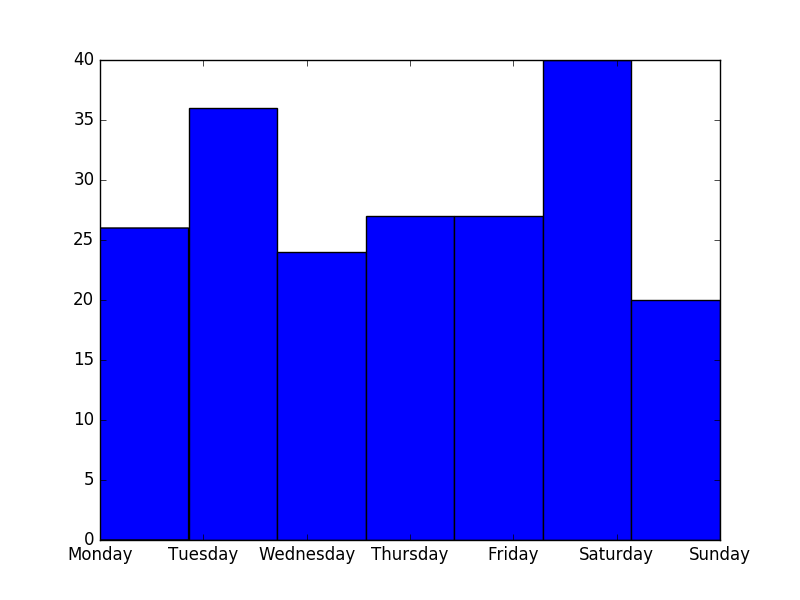
\includegraphics[width=4.16667in]{dow.png}

\subsubsection{\texorpdfstring{More \emph{DataFrame} Manipulation and
Plotting}{More DataFrame Manipulation and Plotting}}\label{more-dataframe-manipulation-and-plotting}

\texttt{DataFrame}s and \texttt{numpy} give us other ways to manipulate
data. For example, we can plot a histogram of the ages of violators like
this:

\begin{verbatim}
>>> ages = data['Cited Person Age'].astype(int)
>>> fig = plt.figure()
>>> ax = fig.add_subplot(1, 1, 1)
>>> plt.hist(ages, bins=np.max(ages) - np.min(ages))
>>> plt.show()
\end{verbatim}

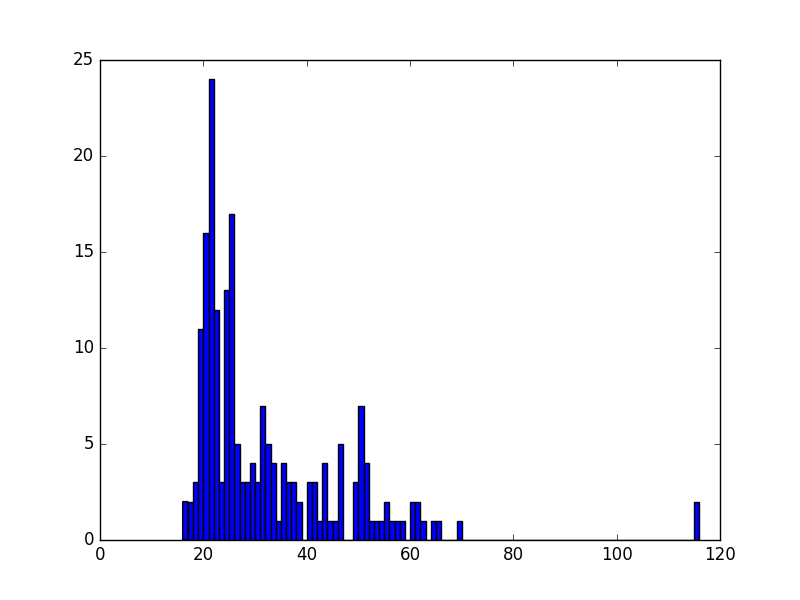
\includegraphics[width=4.16667in]{ages.png}

Surprisingly, we see some 116 year-old violators! This is probably an
error in the data, so we can remove these data points easily and plot
the histogram again:

\begin{verbatim}
>>> ages = ages[ages < 100]
>>> fig = plt.figure()
>>> ax = fig.add_subplot(1, 1, 1)
>>> plt.hist(ages, bins=np.max(ages) - np.min(ages))
>>> plt.show()
\end{verbatim}

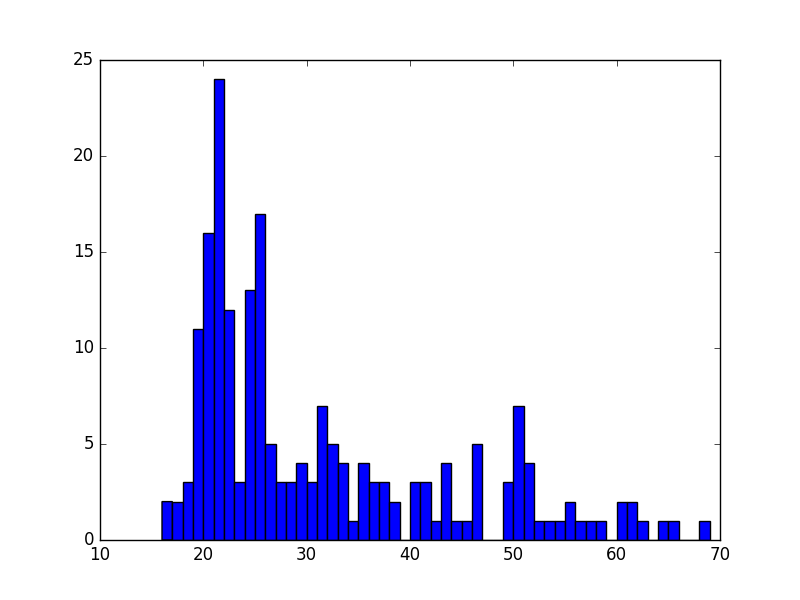
\includegraphics[width=4.16667in]{ages-filtered.png}

\subsubsection{Saving Plots to PDF}\label{saving-plots-to-pdf}

Oftentimes, you will want to save your \texttt{matplotlib} graph as a
PDF or an SVG file instead of just viewing it on your screen. For both,
we need to create a \texttt{figure} and plot the histogram as before:

\begin{verbatim}
>>> fig = plt.figure()
>>> ax = fig.add_subplot(1, 1, 1)
>>> plt.hist(ages, bins=np.max(ages) - np.min(ages))
\end{verbatim}

Then, instead of calling \texttt{plt.show()} we can invoke
\texttt{plt.savefig()} to save as SVG:

\begin{verbatim}
>>> plt.savefig('hist.svg')
\end{verbatim}

If we want to save the figure as PDF instead, we need to use the
\texttt{PdfPages} module together with \texttt{savefig()}:

\begin{verbatim}
>>> import matplotlib.patches as mpatches
>>> from matplotlib.backends.backend_pdf import PdfPages   
>>> pp = PdfPages('hist.pdf')
>>> fig.savefig(pp, format='pdf')
>>> pp.close()
\end{verbatim}

\subsubsection{Next Steps and Exercises}\label{next-steps-and-exercises}

There is a lot more to working with \texttt{pandas}, \texttt{numpy} and
\texttt{matplotlib} than we can show you here, but hopefully this
example has piqued your curiosity.

Don't worry if you don't understand everything in this example. For a
more detailed explanation on these modules and the examples we did,
please take a look at the tutorials below. The \texttt{numpy} and
\texttt{pandas} tutorials are mandatory if you want to be able to use
these modules, and the \texttt{matplotlib} gallery has many useful code
examples.

\subsection{Summary of Useful
Libraries}\label{summary-of-useful-libraries}

\subsubsection{Numpy}\label{numpy}

\begin{itemize}
\tightlist
\item
  \url{http://www.numpy.org/}
\end{itemize}

According to the Numpy Web page "NumPy is a package for scientific
computing with Python. It contains a powerful N-dimensional array
object, sophisticated (broadcasting) functions, tools for integrating
C/C++ and Fortran code, useful linear algebra, Fourier transform, and
random number capabilities

Tutorial:
\url{https://docs.scipy.org/doc/numpy-dev/user/quickstart.html}

\subsubsection{MatplotLib}\label{matplotlib}

\begin{itemize}
\tightlist
\item
  \url{http://matplotlib.org/}
\end{itemize}

According the the Matplotlib Web page, ``matplotlib is a python 2D
plotting library which produces publication quality figures in a variety
of hardcopy formats and interactive environments across platforms.
matplotlib can be used in python scripts, the python and ipython shell
(ala MATLAB®* or Mathematica®†), web application servers, and six
graphical user interface toolkits.''

Matplotlib Gallery: \url{http://matplotlib.org/gallery.html}

\subsubsection{Pandas}\label{pandas}

\begin{itemize}
\tightlist
\item
  \url{http://pandas.pydata.org/}
\end{itemize}

According to the Pandas Web page, ``Pandas is a library library
providing high-performance, easy-to-use data structures and data
analysis tools for the Python programming language.''

In addition to access to charts via matplotlib it has elementary
functionality for conduction data analysis. Pandas may be very suitable
for your projects.

Tutorial: \url{http://pandas.pydata.org/pandas-docs/stable/10min.html}

Pandas Cheat Sheet:
\url{https://github.com/pandas-dev/pandas/blob/master/doc/cheatsheet/Pandas_Cheat_Sheet.pdf}

\subsection{Other Useful Libraries}\label{other-useful-libraries}

\subsubsection{Scipy}\label{scipy}

\begin{itemize}
\tightlist
\item
  \url{https://www.scipy.org/}
\end{itemize}

According to the SciPy Web page, ``SciPy (pronounced ``Sigh Pie'') is a
Python-based ecosystem of open-source software for mathematics, science,
and engineering. In particular, these are some of the core packages:

\begin{itemize}
\tightlist
\item
  NumPy
\item
  IPython
\item
  Pandas
\item
  Matplotlib
\item
  Sympy
\item
  SciPy library
\end{itemize}

It is thus an agglomeration of useful pacakes and will prbably sufice
for your projects in case you use Python.

\subsubsection{ggplot}\label{ggplot}

\begin{itemize}
\tightlist
\item
  \url{http://ggplot.yhathq.com/}
\end{itemize}

According to the ggplot python Web page ggplot is a plotting system for
Python based on R's ggplot2. It allows to quickly generate some plots
quickly with little effort. Often it may be easier to use than
matplotlib directly.

\subsubsection{seaborn}\label{seaborn}

\url{http://www.data-analysis-in-python.org/t_seaborn.html}

The good library for plotting is called seaborn which is build on top of
matplotlib. It provides high level templates for common statistical
plots.

\begin{itemize}
\tightlist
\item
  Gallery:
  \url{http://stanford.edu/~mwaskom/software/seaborn/examples/index.html}
\item
  Original Tutorial:
  \url{http://stanford.edu/~mwaskom/software/seaborn/tutorial.html}
\item
  Additional Tutorial:
  \url{https://stanford.edu/~mwaskom/software/seaborn/tutorial/distributions.html}
\end{itemize}

\subsubsection{Bokeh}\label{bokeh}

Bokeh is an interactive visualization library with focus on web browsers
for display. Its goal is to provide a similar experience as D3.js

\begin{itemize}
\tightlist
\item
  URL: \url{http://bokeh.pydata.org/}
\item
  Gallery: \url{http://bokeh.pydata.org/en/latest/docs/gallery.html}
\end{itemize}

\subsubsection{pygal}\label{pygal}

Pygal is a simple API to produce graphs that can be easily embedded into
your Web pages. It contains annotations when you hover over data points.
It also allows to present the data in a table.

\begin{itemize}
\tightlist
\item
  URL: \url{http://pygal.org/}
\end{itemize}

\subsubsection{Network and Graphs}\label{network-and-graphs}

\begin{itemize}
\tightlist
\item
  igraph: \url{http://www.pythonforsocialscientists.org/t_igraph.html}
\item
  networkx: \url{https://networkx.github.io/}
\end{itemize}

\subsubsection{REST}\label{rest}

\begin{itemize}
\tightlist
\item
  django REST FRamework \url{http://www.django-rest-framework.org/}
\item
  flask
  \url{https://blog.miguelgrinberg.com/post/designing-a-restful-api-with-python-and-flask}
\item
  requests
  \url{https://realpython.com/blog/python/api-integration-in-python/}
\item
  urllib2
  \url{http://rest.elkstein.org/2008/02/using-rest-in-python.html} (not
  recommended)
\item
  web
  \url{http://www.dreamsyssoft.com/python-scripting-tutorial/create-simple-rest-web-service-with-python.php}
  (not recommended)
\item
  bottle \url{http://bottlepy.org/docs/dev/index.html}
\item
  falcon \url{https://falconframework.org/}
\item
  eve \url{http://python-eve.org/}
\item
  \url{https://code.tutsplus.com/tutorials/building-rest-apis-using-eve--cms-22961}
\end{itemize}

\subsection{Other Examples}\label{other-examples}

\begin{itemize}
\tightlist
\item
  Fingerprint Analysis \textless{}python\_lesson1\textgreater{}
\end{itemize}

\section{REST with Eve}\label{rest-with-eve}

\subsection{Overview of REST}\label{overview-of-rest}

REST stands for REpresentational State Transfer. REST is an architecture
style for designing networked applications. It is based on stateless,
client-server, cacheable communications protocol. Although not based on
http, in most cases, the HTTP protocol is used. In contrast to what some
others write or say, REST is not a \emph{standard}.

RESTful applications use HTTP requests to:

\begin{itemize}
\tightlist
\item
  post data: while creating and/or updating it,
\item
  read data: while making queries, and
\item
  delete data.
\end{itemize}

Hence REST uses HTTP for the four CRUD operations:

\begin{itemize}
\tightlist
\item
  Create
\item
  Read
\item
  Update
\item
  Delete
\end{itemize}

As part of the HTTP protocol we have methods such as GET, PUT, POST, and
DELETE. These methods can than be used to implement a REST service. As
REST introduces collections and items we need to implement the CRUD
functions for them. The semantics is explained in the Table
illustrationg how to implement them with HTTP methods.

Source:
\url{https://en.wikipedia.org/wiki/Representational_state_transfer}

\subsection{REST and eve}\label{rest-and-eve}

Now that we have outlined the basic functionality that we need, we lke
to introduce you to Eve that makes this process rather trivial. We will
provide you with an implementation example that showcases that we can
create REST services without writing a single line of code. The code for
this is located at \url{https://github.com/cloudmesh/rest}

This code will have a master branch but will also have a dev branch in
which we will add gradually more objects. Objects in the dev branch will
include:

\begin{itemize}
\tightlist
\item
  virtual directories
\item
  virtual clusters
\item
  job sequences
\item
  inventories
\end{itemize}

;You may want to check our active development work in the dev branch.
However for the purpose of this class the master branch will be
sufficient.

\subsubsection{Installation}\label{installation}

First we havt to install mongodb. The instalation will depend on your
operating system. For the use of the rest service it is not important to
integrate mongodb into the system upon reboot, which is focus of many
online documents. However, for us it is better if we can start and stop
the services explicitly for now.

On ubuntu, you need to do the following steps:

\begin{verbatim}
TO BE CONTRIBUTED BY THE STUDENTS OF THE CLASS as homework
\end{verbatim}

On windows 10, you need to do the following steps:

\begin{verbatim}
TO BE CONTRIBUTED BY THE STUDENTS OF THE CLASS as homework, if you
elect Windows 10. YOu could be using the online documentation
provided by starting it on Windows, or rinning it in a docker container.
\end{verbatim}

On OSX you can use homebrew and install it with:

\begin{verbatim}
brew update
brew install mongodb
\end{verbatim}

\begin{description}
\item[In future we may want to add ssl authentication in which case you
may]
need to install it as follows:
\end{description}

brew install mongodb --with-openssl

\subsubsection{Starting the service}\label{starting-the-service}

We have provided a convenient Makefile that currently only works for
OSX. It will be easy for you to adapt it to Linux. Certainly you can
look at the targes in the makefile and replicate them one by one.
Improtaht targest are deploy and test.

When using the makefile you can start the services with:

\begin{verbatim}
make deploy
\end{verbatim}

IT will start two terminals. IN one you will see the mongo service, in
the other you will see the eve service. The eve service will take a file
called sample.settings.py that is base on sample.json for the start of
the eve service. The mongo servide is configured in suc a wahy that it
only accepts incimming connections from the local host which will be
suffiicent fpr our case. The mongo data is written into the
\$USER/.cloudmesh directory, so make sure it exists.

To test the services you can say:

\begin{verbatim}
make test
\end{verbatim}

YOu will se a number of json text been written to the screen.

\subsection{Creating your own objects}\label{creating-your-own-objects}

The example demonstrated how easy it is to create a mongodb and an eve
rest service. Now lets use this example to creat your own. FOr this we
have modified a tool called evegenie to install it onto your system.

The original documentation for evegenie is located at:

\begin{itemize}
\tightlist
\item
  \url{http://evegenie.readthedocs.io/en/latest/}
\end{itemize}

However, we have improved evegenie while providing a commandline tool
based on it. The improved code is located at:

\begin{itemize}
\tightlist
\item
  \url{https://github.com/cloudmesh/evegenie}
\end{itemize}

You clone it and install on your system as follows:

\begin{verbatim}
cd ~/github
git clone https://github.com/cloudmesh/evegenie
cd evegenie
python setup.py install
pip install .
\end{verbatim}

This shoudl install in your system evegenie. YOu can verify this by
typing:

\begin{verbatim}
which evegenie
\end{verbatim}

If you see the path evegenie is installed. With evegenie installed its
usaage is simple:

\begin{verbatim}
$ evegenie

Usage:
    evegenie --help
    evegenie FILENAME
\end{verbatim}

It takes a json file as input and writes out a settings file for the use
in eve. Lets assume the file is called sample.json, than the settings
file will be called sample.settings.py. Having the evegenie programm
will allow us to generate the settings files easily. You can include
them into your project and leverage the Makefile targets to start the
services in your project. In case you generate new objects, make sure
you rerun evegenie, kill all previous windows in whcih you run eve and
mongo and restart. In case of changes to objects that you have designed
and run previously, you need to also delete the mongod database.

\subsection{Towards cmd5 extensions to manage eve and
mongo}\label{towards-cmd5-extensions-to-manage-eve-and-mongo}

Naturally it is of advantage to have in cms administration commands to
manage mongo and eve from cmd instead of targets in the Makefile. Hence,
we \textbf{propose} that the class develops such an extension. We will
create in the repository the extension called admin and hobe that
students through collaborative work and pull requests complete such an
admin command.

The proposed command is located at:

\begin{itemize}
\tightlist
\item
  \url{https://github.com/cloudmesh/rest/blob/master/cloudmesh/ext/command/admin.py}
\end{itemize}

It will be up to the class to implement such a command. Please
coordinate with each other.

The implementation based on what we provided in the Make file seems
straight forward. A great extensinion is to load the objects definitions
or eve e.g. settings.py not from the class, but forma place in
.cloudmesh. I propose to place the file at:

\begin{verbatim}
.cloudmesh/db/settings.py
\end{verbatim}

the location of this file is used whne the Service class is initialized
with None. Prior to starting the service the file needs to be copied
there. This could be achived with a set commad.

\FILENAME\
\section{Visualization}

\begin{figure}
\centering
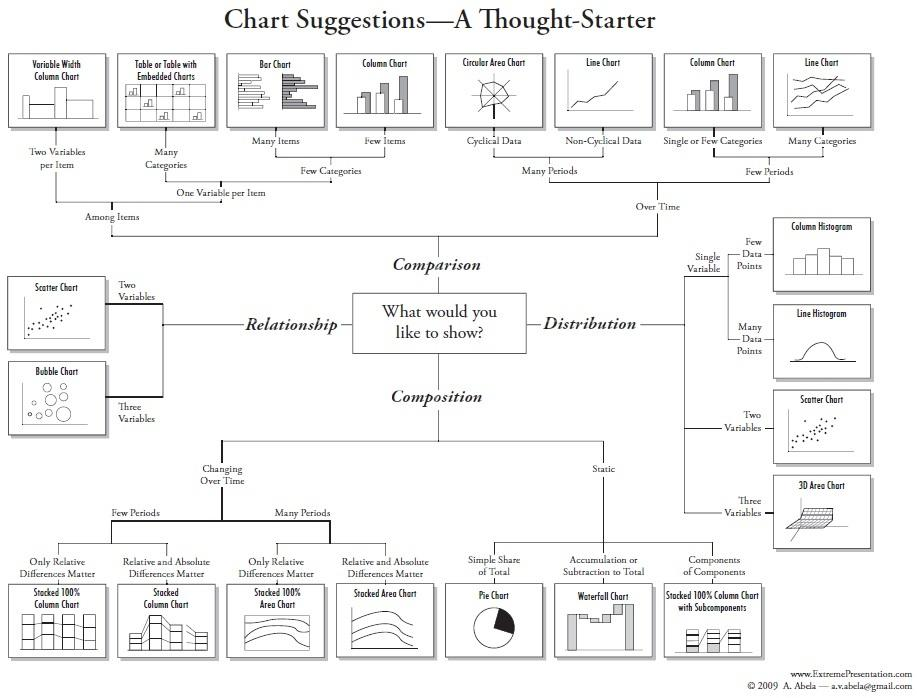
\includegraphics[width=\textwidth]{images/which-chart-when.jpeg}
\caption{Visualisation}
\end{figure}

\URL{https://github.com/d3/d3/wiki/Gallery}

\FILENAME\
\section{Software Projects}\label{software-projects}

\textbf{Contents}

Please read the information in the overview page at

\begin{itemize}

\item
  \url{http://bdaafall2016.readthedocs.io/en/latest/overview.html\#software-project}
\end{itemize}

After doing so please return to this page. Identify a project suitable
for this class, propose it and work on it.

There are several categories of software projects, which are detailed in
lower sections:

\begin{enumerate}

\item
  Deployment
\item
  Analytics
\end{enumerate}

You may propose a project in one of these categories, if you are doing a
software projects.

These are non-trivial project and involve substantial work. Many
students vastly underestimate the difficulty and the amount of time
required. This is the reason why the project assignment is early on in
the semester so you have ample time to propose and work on it. If you
start the project 2 weeks before December (Note the early due data) We
assume you may not finish.

\subsection{Common Requirements}\label{common-requirements}

All software projects must:

\begin{enumerate}
\item
  Be submitted via gitlab (a repository will be created for you)
\item
  Be reproducibly deployed

  Assume you are given a username and a set of IP addresses. From this
  starting point, you should be able to deploy everything in a single
  command line invocation.

  Do not assume that the username or IP address will be the ones you use
  during development and testing.
\item
  Provide a report in the \texttt{docs/report} directory

  LaTeX or Word may be used. Include the original sources as well as a
  PDF called \texttt{report.pdf} (See overview-software-project for
  additional details on the report format. You will be using 2 column
  ACM format we have used before.)
\item
  Provide a properly formatted \texttt{README.rst} or \texttt{README.md}
  in the root directory

  The README should have the following sections:

  \begin{itemize}

  \item
    Authors: list the authors
  \item
    Project Type: one of ``Deployment'', ``Analytics''
  \item
    Problem: describe the task and/or problem
  \item
    Requirements: describe your assumptions and requirements for
    deployment/running. This should include any software requirements
    with a link to their webpage. Also indicate which versions you have
    developed/tested with.
  \item
    Running: describe the steps needed to deploy and run
  \item
    Acknowledgements: provide proper attribution to any websites, or
    code you may have used or adapted
  \end{itemize}

  \begin{description}
  \item[in the past we got projects that had 10 pages]
  installation instructions. Certainly that is not good and you will get
  point deductions. The installation should be possible in a couple of
  lines. A nice example is the installation of the development software
  in the ubuntu vm. Naturally you can use other technologies, other than
  ansible. Shell scrips, makefiles, python scripts are all acceptable.
  \end{description}
\item
  A \texttt{LICENSE} file (this should be the \texttt{LICENSE} for
  Apache License Version 2.0)
\item
  All figures should include labels with the following format:
  \texttt{label\ (units)}.

  For example:

  \begin{itemize}

  \item
    \texttt{distance\ (meters)}
  \item
    \texttt{volume\ (liters)}
  \item
    \texttt{cost\ (USD)}
  \end{itemize}
\item
  All figures should have a caption describing what the measurement is,
  and a summary of the conclusions drawn.

  For example:

  \begin{quote}
  This shows how A changes with regards to B, indicating that under
  conditions X, Y, Z, Alpha is 42 times better than otherwise.
  \end{quote}
\end{enumerate}

\subsection{Deployment Projects}\label{deployment-projects}

Deployment projects focuses on automated software deployments on
multiple nodes using automation tools such as Ansible, Chef, Puppet,
Salt, or Juju. You are also allowed to use shell scripts, pdsh, vagrant,
or fabric. For example, you could work on deploying Hadoop to a cluster
of several machines. Use of Ansible is recommended and supported. Other
tools such as Chef, Puppet, etc, will not be supported.

Note that it is not sufficient to merely deploy the software on the
cluster. You must also demonstrate the use of the cluster by running
some program on it and show the utilization of your entire cluster. You
should also benchmark the deployment and running of your demonstration
on several sizes of a cluster (eg 1, 3, 6, 10 nodes) (Note that these
numbers are for example only).

We expect to see figures showing times for each (deployment, running)
pair on for each cluster size, with error bars. This means that you need
to run each benchmark multiple times (at least three times) in order to
get the error bars. You should also demonstrate cluster utilization for
each cluster size.

The program used for demonstration can be simple and straightforward.
This is not the focus of this type of project.

\subsection{IaaS}\label{iaas}

It is allowable to use

\begin{itemize}

\item
  virtualbox
\item
  chameleon cloud
\item
  futuresystems
\item
  AWS (your own cost)
\item
  Azure (your own cost)
\end{itemize}

for your projects. Note that on powerful desktop machines even
virtualbox can run multiple vms. Use of docker is allowed, but you must
make sure to use docker properly. In the past we had students that used
docker but did not use it in the way it was designed for. Use of docker
swarm is allowed.

\subsubsection{Requirements}\label{requirements}

Deployment projects must include a repeatable deployment framework that
uses cmd5 and ansible. When using ansible it should be called from a
custoom cmd5 program.

\subsubsection{Example projects}\label{example-projects}

See also
\url{https://docs.google.com/document/d/1KylDsRBmVbCZSqGpRbzYwdzUGKFi92bkATwU03of5gw}

\begin{itemize}

\item
  deploy Apache Spark on top of Hadoop
\item
  deploy Apache Pig on top of Hadoop
\item
  deploy Apache Storm
\item
  deploy Apache Flink
\item
  deploy a Tensorflow cluster
\item
  deploy a PostgreSQL cluster
\item
  deploy a MongoDB cluster
\item
  deploy a CouchDB cluster
\item
  deploy a Memcached cluster
\item
  deploy a MySQL cluster
\item
  deploy a Redis cluster
\item
  deploy a Mesos cluster
\item
  deploy a Hadoop cluster
\item
  deploy a docker swarm cluster
\item
  deploy NIST Fingerprint Matching
\item
  deploy NIST Human Detection and Face Detection
\item
  deploy NIST Live Twitter Analysis
\item
  deploy NIST Big Data Analytics for Healthcare Data and Health
  Informatics
\item
  deploy NIST Data Warehousing and Data mining
\end{itemize}

Deployment projects must have EASY installation setup just as we
demonstrated in the ubuntu image.

A command to manage the deployment must be written using python docopts
that than starts your deployment and allows management of it. You can
than from within this command call whatever other framework you use to
manage it. The docopts manual page should be designed first and
discussed in the team for completeness.

Using argparse and other python commandline interface environments is
not allowed.

Deployment project will not only deply the farmewor, but either provide
a sophisticated benchmark while doing a simple analysis using the
deployed software.

\subsection{Analytics Projects}\label{analytics-projects}

Analytics projects focus on data exploration. For this type of projects,
you should focus on analysis of a dataset (see datasets for starting
points). The key here is to take a dataset and extract some meaningful
information from in using tools such as \texttt{scikit-learn},
\texttt{mllib}, or others. You should be able to provide graphs,
descriptions for your graphs, and argue for conclusions drawn from your
analysis.

Your deployment should handle the process of downloading and installing
the required datasets and pushing the analysis code to the remote node.
You should provide instructions on how to run and interpret your
analysis code in your README.

\subsubsection{Requirements}\label{requirements-1}

An analytocs project may focus on a sophisticated and academically
correct usage of an analytics of data. It must be significant and not
just a simple replication of what others have done before.

\subsubsection{Example projects}\label{example-projects-1}

\begin{itemize}

\item
  analysis of US Census data
\item
  analysis of Uber ride sharing GPS data
\item
  analysis of Health Care data
\item
  analysis of images for Human Face detection
\item
  analysis of streaming Twitter data
\item
  analysis of airline prices, flights, etc
\item
  analysis of network graphs (social networks, disease networks, protein
  networks, etc)
\item
  analysis of music files for recommender engines
\item
  analysis of NIST Fingerprint Matching
\item
  analysis of NIST Human Detection and Face Detection
\item
  analysis of NIST Live Twitter Analysis
\item
  analysis of NIST Big Data Analytics for Healthcare Data and Health
  Informatics
\item
  analysis of NIST Data Warehousing and Data mining
\item
  author disambiguity problem in academic papers
\item
  application of a k-means algorithm
\item
  application of a MDS
\end{itemize}

\subsection{Project Idea: World wide road
kill}\label{project-idea-world-wide-road-kill}

This project can also be executed as bonus project to gather information
about the feasability of existing databases.

It would be important to identify also how to potentially merge these
databases into a single world map and derive statistics from them. This
project can be done on your local machines. Not more than 6 people can
work on this.

Identify someone that has experience with android and/or iphone
programming Design an application that preferably works on iphone and
android that allows a user while driving to

\begin{itemize}

\item
  call a number to report roadkill via voice and submitting the gps
  coordinates
\item
  have a button on the phone that allows the gps coordinates to be
  collected and allow upload either live, or when the user presses
  another butten.
\item
  have provisions in the application that allow you to augment the data
\item
  have an html page that displays the data
\item
  test it out within users of this class (remember we have world wide
  audience)
\end{itemize}

Make sure the app is ready early so others can test and use it and you
can collect data.

Before starting the project identify if such an application already
exists.

If more than 6 people sign up we may build a second group doing
something similar, maybe potholes ..

Gregor would like to get this project or at least the database search
query staffed.

\subsection{Project Idea: Author disambiguty
problem}\label{project-idea-author-disambiguty-problem}

Given millions of publications how do we identify if an author of paper
a with the name Will Smith is the sam as the author of paper 2 with the
name Will Smith, or William Smith, or W. Smith. AUthor databases are
either provided in bibtex format, or a database that can not be shared
outside of this class. YOu may have to add additional information from
IEEE explorer, rsearch gate, ISI, or other online databases.

Identify further issues and discuss solutions to them. Example, an
author name changes, the author changes the institution.

Do a comprehensive literature review

Some ideas:

\begin{itemize}

\item
  Develop a graph view application in JS that showcases dependencies
  between coauthors, institutions
\item
  Derive probabilities for the publications written by an auther given
  they are the same
\item
  Utilize dependency graphs as given by online databases
\item
  Utilize the and or topic/abstarct/full text to identify similarity
\item
  Utilize keywords in the title
\item
  Utilize refernces of the paper
\item
  Prepare some vizualization of your result
\item
  Prepare som interactive vizualization
\end{itemize}

A possible good start is a previous project published at

\begin{itemize}

\item
  \url{https://github.com/scienceimpact/bibliometric}
\end{itemize}

There are also some screenshots available:

\begin{itemize}

\item
  \url{https://github.com/scienceimpact/bibliometric/blob/master/Project\%20Screenshots/Relationship_Authors_Publications.PNG}
\item
  \url{https://github.com/scienceimpact/bibliometric/blob/master/Project\%20Screenshots/Relationship_Authors_Publications2_Clusters.PNG}
\end{itemize}


\end{comment}

%Application sections
\begin{comment}


\chapter{Health Informatics Case Study}

\FILENAME

\slides{Health}{131}{Health Informatics}{https://drive.google.com/open?id=0B6wqDMIyK2P7UGRJNmlkYkNkQk0}

This section starts by discussing general aspects of Big Data and Health
including data sizes, different areas including genomics, EBI, radiology
and the Quantified Self movement. We review current state of health care
and trends associated with it including increased use of Telemedicine.
We summarize an industry survey by GE and Accenture and an impressive
exemplar Cloud-based medicine system from Potsdam. We give some details
of big data in medicine. Some remarks on Cloud computing and Health
focus on security and privacy issues.

We survey an April 2013 McKinsey report on the Big Data revolution in US
health care; a Microsoft report in this area and a European Union report
on how Big Data will allow patient centered care in the future. Examples
are given of the Internet of Things, which will have great impact on
health including wearables. A study looks at 4 scenarios for healthcare
in 2032. Two are positive, one middle of the road and one negative. The
final topic is Genomics, Proteomics and Information Visualization.

\section{Big Data and Health}\label{big-data-and-health}

This lesson starts with general aspects of Big Data and Health including
listing subareas where Big data important. Data sizes are given in
radiology, genomics, personalized medicine, and the Quantified Self
movement, with sizes and access to European Bioinformatics Institute.

\video{Health}{10:02}{Big Data and Health}{https://www.youtube.com/watch?v=ZkM-yZJQ1Cg} 

\section{Status of Healthcare Today}

This covers trends of costs and type of healthcare with low cost genomes
and an aging population. Social media and government Brain initiative.

\video{Health}{16:09}{Status of Healthcare Today}{https://www.youtube.com/watch?v=x9TpdMBqYrk} 

\section{Telemedicine (Virtual Health)}

This describes increasing use of telemedicine and how we tried and
failed to do this in 1994.

\video{Health}{8:21}{Telemedicine}{https://www.youtube.com/watch?v=Pe4CVXQaL_U} 

\begin{comment}
\section{Big Data and Healthcare Industry}

Summary of an industry survey by GE and Accenture.

\video{Health}{10:02}{Big Data and Healthcare Indusry}{https://www.youtube.com/watch?v=64YOUnRJVZU}
\end{comment}

\section{Medical Big Data in the Clouds}

An impressive exemplar Cloud-based medicine system from Potsdam.

\video{Health}{15:02}{Medical Big Data in the Clouds}{https://www.youtube.com/watch?v=GldSVijkJcM} 


\subsection{Medical image Big Data}\label{medical-image-big-data}

\video{Health}{6:33}{Midical Image Big Data}{https://www.youtube.com/watch?v=GOcVtwx2R2k} 

\subsection{Clouds and Health}\label{clouds-and-health}

\video{Health}{4:35}{Clouds and Health}{http://youtu.be/9Whkl_UPS5g}


\subsection{McKinsey Report on the big-data revolution in US health
  care}

This lesson covers 9 aspects of the McKinsey report. These are the
convergence of multiple positive changes has created a tipping point for
innovation; Primary data pools are at the heart of the big data
revolution in healthcare; Big data is changing the paradigm: these are
the value pathways; Applying early successes at scale could reduce US
healthcare costs by \$300 billion to \$450 billion; Most new big-data
applications target consumers and providers across pathways; Innovations
are weighted towards influencing individual decision-making levers; Big
data innovations use a range of public, acquired, and proprietary data
types; Organizations implementing a big data transformation should
provide the leadership required for the associated cultural
transformation; Companies must develop a range of big data capabilities.

\video{Health}{14:53}{McKinsey Report}{https://www.youtube.com/watch?v=fu-TWnIk980} 

\subsection{Microsoft Report on Big Data in Health}

This lesson identifies data sources as Clinical Data, Pharma \& Life
Science Data, Patient \& Consumer Data, Claims \& Cost Data and
Correlational Data. Three approaches are Live data feed, Advanced
analytics and Social analytics.

\video{Health}{2:26}{Microsoft Report on Big Data in Health}{http://youtu.be/PjffvVgj1PE}


\subsection{EU Report on Redesigning health in Europe for 2020}

This lesson summarizes an EU Report on Redesigning health in Europe for
2020. The power of data is seen as a lever for change in My Data, My
decisions; Liberate the data; Connect up everything; Revolutionize
health; and Include Everyone removing the current correlation between
health and wealth.


\video{Health}{5:00}{EU Report on Redesigning health in Europe for 2020}{http://youtu.be/9mbt_ZSs0iw}


\subsection{Medicine and the Internet of Things}

The Internet of Things will have great impact on health including
telemedicine and wearables. Examples are given.

\video{Health}{8:17}{Medicine and the Internet of Things}{https://www.youtube.com/watch?v=Jk3EeFzZnuU}


\subsection{Extrapolating to 2032}

A study looks at 4 scenarios for healthcare in 2032. Two are positive,
one middle of the road and one negative.

\video{Health}{15:13}{Extrapolating to 2032}{https://www.youtube.com/watch?v=a5G4HACeokg} 


\subsection{Genomics, Proteomics and Information Visualization}

A study of an Azure application with an Excel frontend and a cloud BLAST
backend starts this lesson. This is followed by a big data analysis of
personal genomics and an analysis of a typical DNA sequencing analytics
pipeline. The Protein Sequence Universe is defined and used to motivate
Multi dimensional Scaling MDS. Sammon's method is defined and its use
illustrated by a metagenomics example. Subtleties in use of MDS include
a monotonic mapping of the dissimilarity function. The application to
the COG Proteomics dataset is discussed. We note that the MDS approach
is related to the well known chisq method and some aspects of nonlinear
minimization of chisq (Least Squares) are discussed.

\video{Health}{6:56}{Genomics, Proteomics and  Information Visualization}{https://www.youtube.com/watch?v=zGzBtxq1ZRE}

\begin{comment}
\video{Health}{6:56}{ CC) Genomics, Proteomics and  Information Visualization}{https://drive.google.com/file/d/0B5plU-u0wqMoVzduODM0Z2dFYWM/view?usp=sharing}
\end{comment}

Next we continue the discussion of the COG Protein Universe introduced
in the last lesson. It is shown how Proteomics clusters are clearly seen
in the Universe browser. This motivates a side remark on different
clustering methods applied to metagenomics. Then we discuss the
Generative Topographic Map GTM method that can be used in dimension
reduction when original data is in a metric space and is in this case
faster than MDS as GTM computational complexity scales like N not N
squared as seen in MDS.

Examples are given of GTM including an application to topic models in
Information Retrieval. Indiana University has developed a deterministic
annealing improvement of GTM. 3 separate clusterings are projected for
visualization and show very different structure emphasizing the
importance of visualizing results of data analytics. The final slide
shows an application of MDS to generate and visualize phylogenetic
trees.

\TODO{These two videos need to be uploaded to youtube}

\video{Health}{10:33}{Genomics, Proteomics and Information Visualization I}{https://drive.google.com/file/d/0B5plU-u0wqMobXdEQWRHWl95UTA/view?usp=sharing}

\video{Health}{7:41}{Genomics, Proteomics and Information Visualization: II}{https://drive.google.com/file/d/0B5plU-u0wqModlhmdVUwdGlQNTA/view?usp=sharing}

\slides{Health}{131}{Proteomics and Information Visualization}{https://drive.google.com/open?id=0B8936_ytjfjmX0lEMWhMX2kwRHc}
  


\section{Resources}

\TODO{These resources have not all been checked to see if they still
  exist this is curretnly in progress}

\begin{itemize}
\item
  \url{https://wiki.nci.nih.gov/display/CIP/CIP+Survey+of+Biomedical+Imaging+Archives}
\item
  \url{http://grids.ucs.indiana.edu/ptliupages/publications/Where\%20does\%20all\%20the\%20data\%20come\%20from\%20v7.pdf}
\item
  \url{http://www.ieee-icsc.org/ICSC2010/Tony\%20Hey\%20-\%2020100923.pdf}
\item
  \url{http://quantifiedself.com/larry-smarr/}
\item
  \url{http://www.ebi.ac.uk/Information/Brochures/}
\item
  \url{http://www.kpcb.com/internet-trends}
\item
  \url{http://www.slideshare.net/drsteventucker/wearable-health-fitness-trackers-and-the-quantified-self}
\item
  \url{http://www.siam.org/meetings/sdm13/sun.pdf}
\item
  \url{http://en.wikipedia.org/wiki/Calico_\%28company\%29}
\item
  \url{http://www.slideshare.net/GSW_Worldwide/2015-health-trends}
\item
  \url{http://www.accenture.com/SiteCollectionDocuments/PDF/Accenture-Industrial-Internet-Changing-Competitive-Landscape-Industries.pdf}
\item
  \url{http://www.slideshare.net/schappy/how-realtime-analysis-turns-big-medical-data-into-precision-medicine}
\item
  \url{http://medcitynews.com/2013/03/the-body-in-bytes-medical-images-as-a-source-of-healthcare-big-data-infographic/}
\item
  \url{http://healthinformatics.wikispaces.com/file/view/cloud_computing.ppt}
\item
  \url{https://www.mckinsey.com/~/media/mckinsey/industries/healthcare%20systems%20and%20services/our%20insights/the%20big%20data%20revolution%20in%20us%20health%20care/the_big_data_revolution_in_healthcare.ashx}
\begin{comment}
\item
  \url{https://partner.microsoft.com/download/global/40193764}
\end{comment}
\item
  \url{https://ec.europa.eu/eip/ageing/file/353/download_en?token=8gECi1RO}
\item
  \url{http://www.kpcb.com/internet-trends}
\begin{comment}
\item
  \url{http://www.liveathos.com/apparel/app}
\end{comment}
\item
  \url{http://debategraph.org/Poster.aspx?aID=77}
\begin{comment}
\item
  \url{http://www.oerc.ox.ac.uk/downloads/presentations-from-events/microsoftworkshop/gannon}
\end{comment}
\item
  \url{http://www.delsall.org}
\item
  \url{http://salsahpc.indiana.edu/millionseq/mina/16SrRNA_index.html}
\item
  \url{http://www.geatbx.com/docu/fcnindex-01.html}
\item
  \url{https://wiki.nci.nih.gov/display/CIP/CIP+Survey+of+Biomedical+Imaging+Archives}
\item
  \url{http://grids.ucs.indiana.edu/ptliupages/publications/Where\%20does\%20all\%20the\%20data\%20come\%20from\%20v7.pdf}
\item
  \url{http://www.ieee-icsc.org/ICSC2010/Tony\%20Hey\%20-\%2020100923.pdf}
\item
  \url{http://quantifiedself.com/larry-smarr/}
\item
  \url{http://www.ebi.ac.uk/Information/Brochures/}
\item
  \url{http://www.kpcb.com/internet-trends}
\item
  \url{http://www.slideshare.net/drsteventucker/wearable-health-fitness-trackers-and-the-quantified-self}
\item
  \url{http://www.siam.org/meetings/sdm13/sun.pdf}
\item
  \url{http://en.wikipedia.org/wiki/Calico_\%28company\%29}
\item
  \url{http://www.slideshare.net/GSW_Worldwide/2015-health-trends}
\item
  \url{http://www.accenture.com/SiteCollectionDocuments/PDF/Accenture-Industrial-Internet-Changing-Competitive-Landscape-Industries.pdf}
\item
  \url{http://www.slideshare.net/schappy/how-realtime-analysis-turns-big-medical-data-into-precision-medicine}
\item
  \url{http://medcitynews.com/2013/03/the-body-in-bytes-medical-images-as-a-source-of-healthcare-big-data-infographic/}
\item
  \url{http://healthinformatics.wikispaces.com/file/view/cloud_computing.ppt}
\item
  \url{http://www.mckinsey.com/~/media/McKinsey/dotcom/Insights/Health\%20care/The\%20big-data\%20revolution\%20in\%20US\%20health\%20care/The\%20big-data\%20revolution\%20in\%20US\%20health\%20care\%20Accelerating\%20value\%20and\%20innovation.ashx}
\item
  \url{https://partner.microsoft.com/download/global/40193764}
\item
  \url{http://ec.europa.eu/information_society/activities/health/docs/policy/taskforce/redesigning_health-eu-for2020-ehtf-report2012.pdf}
\item
  \url{http://www.kpcb.com/internet-trends}
\item
  \url{http://www.liveathos.com/apparel/app}
\item
  \url{http://debategraph.org/Poster.aspx?aID=77}
\item
  \url{http://www.oerc.ox.ac.uk/downloads/presentations-from-events/microsoftworkshop/gannon}
\item
  \url{http://www.delsall.org}
\item
  \url{http://salsahpc.indiana.edu/millionseq/mina/16SrRNA_index.html}
\item
  \url{http://www.geatbx.com/docu/fcnindex-01.html}
\end{itemize}



\chapter{e-Commerce and LifeStyle}
\label{c:e-commerce}
\index{e-Commerce}
\index{LifeStyle}

\FILENAME

Recommender systems operate under the hood of such widely recognized
sites as Amazon, eBay, Monster and Netflix where everything is a
recommendation. This involves a symbiotic relationship between vendor
and buyer whereby the buyer provides the vendor with information about
their preferences, while the vendor then offers recommendations tailored
to match their needs. Kaggle competitions h improve the success of the
Netflix and other recommender systems. Attention is paid to models that
are used to compare how changes to the systems affect their overall
performance. It is interesting that the humble ranking has become such a
dominant driver of the world's economy. More examples of recommender
systems are given from Google News, Retail stores and in depth Yahoo!
covering the multi-faceted criteria used in deciding recommendations on
web sites.

The formulation of recommendations in terms of points in a space or bag
is given where bags of item properties, user properties, rankings and
users are useful. Detail is given on basic principles behind recommender
systems: user-based collaborative filtering, which uses similarities in
user rankings to predict their interests, and the Pearson correlation,
used to statistically quantify correlations between users viewed as
points in a space of items. Items are viewed as points in a space of
users in item-based collaborative filtering. The Cosine Similarity is
introduced, the difference between implicit and explicit ratings and the
k Nearest Neighbors algorithm. General features like the curse of
dimensionality in high dimensions are discussed. A simple Python k
Nearest Neighbor code and its application to an artificial data set in 3
dimensions is given. Results are visualized in Matplotlib in 2D and with
Plotviz in 3D. The concept of a training and a testing set are
introduced with training set pre labeled. Recommender system are used to
discuss clustering with k-means based clustering methods used and their
results examined in Plotviz. The original labelling is compared to
clustering results and extension to 28 clusters given. General issues in
clustering are discussed including local optima, the use of annealing to
avoid this and value of heuristic algorithms.

\section{Recommender Systems}
\index{Recommender Systems}

We introduce Recommender systems as an optimization technology used in a
variety of applications and contexts online. They operate in the
background of such widely recognized sites as Amazon, eBay, Monster and
Netflix where everything is a recommendation. This involves a symbiotic
relationship between vendor and buyer whereby the buyer provides the
vendor with information about their preferences, while the vendor then
offers recommendations tailored to match their needs, to the benefit of
both.

There follows an exploration of the Kaggle competition site, other
recommender systems and Netflix, as well as competitions held to improve
the success of the Netflix recommender system. Finally attention is paid
to models that are used to compare how changes to the systems affect
their overall performance. It is interesting how the humble ranking has
become such a dominant driver of the world's economy.

\slides{Lifestyle}{Recommender}{45}{https://drive.google.com/open?id=0B6wqDMIyK2P7YkIwczVfQlJqVG8}{PDF}


\subsection{Recommender Systems as an Optimization Problem}

We define a set of general recommender systems as matching of items to
people or perhaps collections of items to collections of people where
items can be other people, products in a store, movies, jobs, events,
web pages etc. We present this as ``yet another optimization problem''.

\video{Lifestyle}{8:06}{Recommender Systems I}{https://www.youtube.com/watch?v=kO023BIW2dw} 


\subsection{Recommender Systems Introduction}

We give a general discussion of recommender systems and point out that
they are particularly valuable in long tail of tems (to be recommended)
that aren't commonly known. We pose them as a rating system and relate
them to information retrieval rating systems. We can contrast
recommender systems based on user profile and context; the most familiar
collaborative filtering of others ranking; item properties; knowledge
and hybrid cases mixing some or all of these.

\video{Lifestyle}{12:56}{Recommender Systems Introduction}{https://youtu.be/KbjBKrzFYKg}


\subsection{Kaggle Competitions}
\index{Kaggle}

We look at Kaggle competitions with examples from web site. In
particular we discuss an Irvine class project involving ranking jokes.

\video{Lifestyle}{3:36}{Kaggle Competitions: }{https://youtu.be/DFH7GPrbsJA}

\begin{IU}

Please not that we do not accept any projects using kaggle data for
this classs.

\end{IU}

\subsection{Examples of Recommender Systems}

We go through a list of 9 recommender systems from the same Irvine
class.

\video{Lifestyle}{1:00}{Examples of Recommender Systems}{https://youtu.be/1Eh1epQj-EQ}


\subsection{Netflix on Recommender Systems}
\index{Netflix}

We summarize some interesting points from a tutorial from Netflix for
whom `'everything is a recommendation''. Rankings are given in multiple
categories and categories that reflect user interests are especially
important. Criteria used include explicit user preferences, implicit
based on ratings and hybrid methods as well as freshness and diversity.
Netflix tries to explain the rationale of its recommendations. We give
some data on Netflix operations and some methods used in its recommender
systems. We describe the famous Netflix Kaggle competition to improve
its rating system. The analogy to maximizing click through rate is given
and the objectives of optimization are given.

\video{Lifestyle}{14:20}{Netflix on Recommender Systems}{https://www.youtube.com/watch?v=ModhdIT9D24}

Next we go through Netflix's methodology in letting data speak for
itself in optimizing the recommender engine. An example iis given on
choosing self produced movies. A/B testing is discussed with examples
showing how testing does allow optimizing of sophisticated criteria.
This lesson is concluded by comments on Netflix technology and the full
spectrum of issues that are involved including user interface, data, AB
testing, systems and architectures. We comment on optimizing for a
household rather than optimizing for individuals in household.

\video{Lifestyle}{13:04}{Consumer Data Science}{https://youtu.be/B8cjaOQ57LI}



\subsection{Other Examples of Recommender Systems}
\index{Google News}

We continue the discussion of recommender systems and their use in
e-commerce. More examples are given from Google News, Retail stores and
in depth Yahoo! covering the multi-faceted criteria used in deciding
recommendations on web sites. Then the formulation of recommendations in
terms of points in a space or bag is given.

Here bags of item properties, user properties, rankings and users are
useful. Then we go into detail on basic principles behind recommender
systems: user-based collaborative filtering, which uses similarities in
user rankings to predict their interests, and the Pearson correlation,
used to statistically quantify correlations between users viewed as
points in a space of items.

\slides{Lifestyle}{Recommender}{49}{https://drive.google.com/open?id=0B6wqDMIyK2P7UVloVElaZ2FXcTg}{PDF}


We start with a quick recap of recommender systems from previous unit;
what they are with brief examples.

\video{Lifestyle}{5:48}{Recap and Examples of Recommender Systems}{https://www.youtube.com/watch?v=PwS8UE4TDS4}

\subsubsection{Examples of Recommender Systems}

We give 2 examples in more detail: namely Google News and Markdown in
Retail.

\video{Lifestyle}{8:34}{Examples of Recommender Systems}{https://youtu.be/og07mH9fU0M}


\subsubsection{Recommender Systems in Yahoo Use Case
Example}
\index{Yahoo}

We describe in greatest detail the methods used to optimize Yahoo web
sites. There are two lessons discussing general approach and a third
lesson examines a particular personalized Yahoo page with its different
components. We point out the different criteria that must be blended in
making decisions; these criteria include analysis of what user does
after a particular page is clicked; is the user satisfied and cannot
that we quantified by purchase decisions etc. We need to choose
Articles, ads, modules, movies, users, updates, etc to optimize metrics
such as relevance score, CTR, revenue, engagement.These lesson stress
that if though we have big data, the recommender data is sparse. We
discuss the approach that involves both batch (offline) and on-line
(real time) components.

\video{Lifestyle}{8:46}{Recap of Recommender Systems II}{https://youtu.be/FBn7HpGFNvg}

\video{Lifestyle}{10:48}{Recap of Recommender Systems III}{https://youtu.be/VS2Y4lAiP5A}

\video{Lifestyle}{3:21}{Case Study of Recommender systems}{https://youtu.be/HrRJWEF8EfU}


\subsubsection{User-based nearest-neighbor collaborative filtering}
\index{Nearest Neighbor}

Collaborative filtering is a core approach to recommender systems. There
is user-based and item-based collaborative filtering and here we discuss
the user-based case. Here similarities in user rankings allow one to
predict their interests, and typically this quantified by the Pearson
correlation, used to statistically quantify correlations between users.

\video{Lifestyle}{7:20}{User-based nearest-neighbor collaborative filtering I}{https://youtu.be/lsf_AE-8dSk}

\video{Lifestyle}{7:29}{User-based nearest-neighbor collaborative filtering II}{https://youtu.be/U7-qeX2ItPk}


\subsubsection{Vector Space Formulation of Recommender
Systems}
\index{Vector Space}

We go through recommender systems thinking of them as formulated in a
funny vector space. This suggests using clustering to make
recommendations.

\video{Lifestyle}{9:06}{Vector Space Formulation of Recommender Systems new}{https://youtu.be/IlQUZOXlaSU}


\subsection{Resources}

\begin{itemize}

\item
  \url{http://pages.cs.wisc.edu/~beechung/icml11-tutorial/}
\end{itemize}

\section{Item-based Collaborative Filtering and its Technologies}
\index{Filtering}

We move on to item-based collaborative filtering where items are viewed
as points in a space of users. The Cosine Similarity is introduced, the
difference between implicit and explicit ratings and the k Nearest
Neighbors algorithm. General features like the curse of dimensionality
in high dimensions are discussed.

\slides{Lifestyle}{Filtering}{18}{https://drive.google.com/open?id=0B6wqDMIyK2P7UExxVFc5YlpOZ28}{PDF}


\subsection{Item-based Collaborative Filtering}

We covered user-based collaborative filtering in the previous unit. Here
we start by discussing memory-based real time and model based offline
(batch) approaches. Now we look at item-based collaborative filtering
where items are viewed in the space of users and the cosine measure is
used to quantify distances. WE discuss optimizations and how batch
processing can help. We discuss different Likert ranking scales and
issues with new items that do not have a significant number of rankings.

\video{Lifestyle}{11:18}{Item Based Filtering}{https://www.youtube.com/watch?v=HTdYGaOTlFI}

\video{Lifestyle}{7:16}{k Nearest Neighbors and High Dimensional Spaces}{https://youtu.be/SM8EJdAa4mw}


\subsection{k-Nearest Neighbors and High Dimensional Spaces}
\index{k-Nearest Neighbors}

We define the k Nearest Neighbor algorithms and present the Python
software but do not use it. We give examples from Wikipedia and describe
performance issues. This algorithm illustrates the curse of
dimensionality. If items were a real vectors in a low dimension space,
there would be faster solution methods.

\video{Lifestyle}{10:03}{k Nearest Neighbors and High Dimensional Spaces}{https://youtu.be/2NqUsDGQDy8}

\subsection{Resources}

\TODO{These resources have not all been checked to see if they still
  exist this is curretnly in progress}


\begin{itemize}

\item
  \url{http://www.slideshare.net/xamat/building-largescale-realworld-recommender-systems-recsys2012-tutorial}
\item
  \url{http://www.ifi.uzh.ch/ce/teaching/spring2012/16-Recommender-Systems_Slides.pdf}
\item
  \url{https://www.kaggle.com/}
\item
  \url{http://www.ics.uci.edu/~welling/teaching/CS77Bwinter12/CS77B_w12.html}
\item
  Jeff Hammerbacher
  \url{https://berkeleydatascience.files.wordpress.com/2012/01/20120117berkeley1.pdf}
\item
  \url{http://www.techworld.com/news/apps/netflix-foretells-house-of-cards-success-with-cassandra-big-data-engine-3437514/}
\item
  \url{https://en.wikipedia.org/wiki/A/B_testing}
\item
  \url{http://www.infoq.com/presentations/Netflix-Architecture}
\end{itemize}



\chapter{Physics Case Studies}
\index{Physics}


\FILENAME

This section starts by describing the LHC accelerator at CERN and
evidence found by the experiments suggesting existence of a Higgs Boson.
The huge number of authors on a paper, remarks on histograms and Feynman
diagrams is followed by an accelerator picture gallery. The next unit is
devoted to Python experiments looking at histograms of Higgs Boson
production with various forms of shape of signal and various background
and with various event totals. Then random variables and some simple
principles of statistics are introduced with explanation as to why they
are relevant to Physics counting experiments. The unit introduces
Gaussian (normal) distributions and explains why they seen so often in
natural phenomena. Several Python illustrations are given. Random
Numbers with their Generators and Seeds lead to a discussion of Binomial
and Poisson Distribution. Monte-Carlo and accept-reject methods. The
Central Limit Theorem concludes discussion.

\section{Looking for Higgs Particles}
\index{Higgs Particles}

\subsection{Bumps in Histograms,  Experiments and Accelerators}

This unit is devoted to Python and Java experiments looking at
histograms of Higgs Boson production with various forms of shape of
signal and various background and with various event totals. The
lectures use Python but use of Java is described.

\slides{Physics}{20}{Higgs}{https://drive.google.com/open?id=0B8936_ytjfjmYXNoM3ZadGR6QlE}

\sourcecode{Physics}{HiggsClassI-Sloping.py}{examples/physics/mr-higgs/higgs-classI-sloping.py}


\subsection{Particle Counting}

We return to particle case with slides used in introduction and stress
that particles often manifested as bumps in histograms and those bumps
need to be large enough to stand out from background in a statistically
significant fashion.

\video{Physics}{13:49}{Discovery of Higgs Particle}{https://www.youtube.com/watch?v=iaypHlgFyuU}

We give a few details on one LHC experiment ATLAS. Experimental physics
papers have a staggering number of authors and quite big budgets.
Feynman diagrams describe processes in a fundamental fashion.

\video{Physics}{7:38}{Looking for Higgs Particle and Counting Introduction II}{http://youtu.be/UAMzmOgjj7I}

\subsection{Experimental Facilities}

We give a few details on one LHC experiment ATLAS. Experimental physics
papers have a staggering number of authors and quite big budgets.
Feynman diagrams describe processes in a fundamental fashion.

\video{Physics}{9:29}{Looking for Higgs Particle Experiments}{http://youtu.be/BW12d780qT8}

\subsection{Accelerator Picture Gallery of Big Science}

This lesson gives a small picture gallery of accelerators. Accelerators,
detection chambers and magnets in tunnels and a large underground
laboratory used fpr experiments where you need to be shielded from
background like cosmic rays.

\video{Physics}{11:21}{Accelerator Picture Gallery of Big Science}{http://youtu.be/WLJIxWWMYi8}

\subsection{Resources}\label{resources}

\begin{itemize}

\item
  \url{http://grids.ucs.indiana.edu/ptliupages/publications/Where\%20does\%20all\%20the\%20data\%20come\%20from\%20v7.pdf}
\item
  \url{http://www.sciencedirect.com/science/article/pii/S037026931200857X}
\item
  \url{http://www.nature.com/news/specials/lhc/interactive.html}
\end{itemize}

Looking for Higgs Particles: Python Event Counting for Signal and
Background (Part 2)


This unit is devoted to Python experiments looking at histograms of
Higgs Boson production with various forms of shape of signal and various
background and with various event totals.

\slides{Physics}{29}{Higgs II}{https://drive.google.com/open?id=0B8936_ytjfjmUHRpV2g2V28walE}{PDF}

Files:

\sourcecode{Physics}{HiggsClassI-Sloping.py}{examples/physics/mr-higgs/higgs-classI-sloping.py}

\sourcecode{Physics}{HiggsClassIII.py}{examples/physics/number-theory/higgs-classIII.py}

\sourcecode{Physics}{HiggsClassIIUniform.py}{examples/physics/mr-higgs/higgs-classII-uniform.py}


%\subsection{Physics Use Case II 1: Class
%Software}\label{physics-use-case-ii-1-class-software}

%We discuss how this unit uses Java and Python on both a backend server
%(FutureGrid) or a local client. WE point out useful book on Python for
%data analysis. This builds on technology training in Section 3.

%\video{Physics}{9:30}{Higgs Particle Events and Counting}{https://www.youtube.com/watch?v=L8j2qB4lSZ0}

%\begin{WARNING}
%This video contains Java information, but we are no longer using Java in
%this class.
%\end{WARNING}%

\subsection{Event Counting}
\index{Event Counting}

We define \textit{event counting} data collection environments. We discuss
the python and Java code to generate events according to a particular
scenario (the important idea of Monte Carlo data). Here a sloping
background plus either a Higgs particle generated similarly to LHC
observation or one observed with better resolution (smaller measurement
error).

\video{Physics}{7:02}{Event Counting}{http://youtu.be/h8-szCeFugQ}

\subsection{Monte Carlo}
\index{Monte Carlo}

This uses Monte Carlo data both to generate data like the experimental
observations and explore effect of changing amount of data and changing
measurement resolution for Higgs.

\video{Physics}{7:33}{With Python examples of Signal plus Background}{http://youtu.be/bl2f0tAzLj4}

This lesson continues the examination of Monte Carlo data looking at
effect of change in number of Higgs particles produced and in change
in shape of background.

\video{Physics}{7:01}{Change shape of background \& num of Higgs Particles}{http://youtu.be/bw3fd5cfQhk}

\subsection{Resources}\label{resources-1}

\begin{itemize}

\item
  Python for Data Analysis: Agile Tools for Real World Data By Wes
  McKinney, Publisher: O'Reilly Media, Released: October 2012, Pages:
  472.
\item
  \url{http://jwork.org/scavis/api/}
\item
  \url{https://en.wikipedia.org/wiki/DataMelt}
\end{itemize}

\subsection{Random Variables, Physics and
  Normal Distributions}

We introduce random variables and some simple principles of statistics
and explains why they are relevant to Physics counting experiments. The
unit introduces Gaussian (normal) distributions and explains why they
seen so often in natural phenomena. Several Python illustrations are
given. Java is currently not available in this unit.

\slides{Physics}{39}{Higgs}{https://drive.google.com/open?id=0B8936_ytjfjmNWhrS0xadk16SWM}

\sourcecode{Physics}{HiggsClassIII.py}{examples/physics/number-theory/higgs-classIII.py}

\subsection{Statistics Overview and Fundamental Idea: Random
  Variables}
\index{Random Variables}

We go through the many different areas of statistics covered in the
Physics unit. We define the statistics concept of a random variable.

\video{Physics}{8:19}{Random variables and normal distributions}{https://www.youtube.com/watch?v=_sLGyt4qWWk}

\subsection{Physics and Random Variables}


We describe the DIKW pipeline for the analysis of this type of physics
experiment and go through details of analysis pipeline for the LHC ATLAS
experiment. We give examples of event displays showing the final state
particles seen in a few events. We illustrate how physicists decide
whats going on with a plot of expected Higgs production experimental
cross sections (probabilities) for signal and background.

\video{Physics}{8:34}{Physics and Random Variables I}{http://youtu.be/Tn3GBxgplxg}

\video{Physics}{5:50}{Physics and Random Variables II}{http://youtu.be/qWEjp0OtvdA}

\subsection{Statistics of Events with Normal Distributions}
\index{Normal Distributions}

We introduce Poisson and Binomial distributions and define independent
identically distributed (IID) random variables. We give the law of large
numbers defining the errors in counting and leading to Gaussian
distributions for many things. We demonstrate this in Python
experiments.

\video{Physics}{11:25}{Statistics of Events with Normal Distributions}{http://youtu.be/LMBtpWOOQLo}

\subsection{Gaussian Distributions}
\index{Gaussian Distributions}

We introduce the Gaussian distribution and give Python examples of the
fluctuations in counting Gaussian distributions.

\video{Physics}{9:08}{Gaussian Distributions}{http://youtu.be/LWIbPa-P5W0}

\subsection{Using Statistics}
\index{Statistics}

We discuss the significance of a standard deviation and role of biases
and insufficient statistics with a Python example in getting incorrect
answers.

\video{Physics}{14:02}{Using Statistics}{http://youtu.be/n4jlUrGwgic}

\subsection{Resources}

\begin{itemize}

\item
  \url{http://indico.cern.ch/event/20453/session/6/contribution/15?materialId=slides}
\item
  \url{http://www.atlas.ch/photos/events.html}
\item
  \url{https://cms.cern/}
\end{itemize}

\subsection{Random Numbers, Distributions and Central Limit Theorem}
\index{Central Limit Theorem}

We discuss Random Numbers with their Generators and Seeds. It introduces
Binomial and Poisson Distribution. Monte-Carlo and accept-reject methods
are discussed. The Central Limit Theorem and Bayes law concludes
discussion. Python and Java (for student - not reviewed in class)
examples and Physics applications are given.

\slides{Physics}{44}{Higgs III}{https://drive.google.com/open?id=0B8936_ytjfjmTUxkZXVRRmlBSUk}{PDF}

Files:

\sourcecode{Physics}{HiggsClassIII.py}{examples/physics/calculated-dice-roll/higgs-classIV-seeds.py}

\subsubsection{Generators and Seeds}
\index{Generators}
\index{Seeds}

We define random numbers and describe how to generate them on the
computer giving Python examples. We define the seed used to define to
specify how to start generation.

\video{Physics}{6:28}{Higgs Particle Counting Errors}{https://www.youtube.com/watch?v=de4AQ9AFt54}

\video{Physics}{7:10}{Generators and Seeds II}{http://youtu.be/9QY5qkQj2Ag}

\subsubsection{Binomial Distribution}
\index{Binomial Distribution}


We define binomial distribution and give LHC data as an example of where
this distribution valid.

\video{Physics}{12:38}{Binomial Distribution: }{http://youtu.be/DPd-eVI_twQ}

\subsubsection{Accept-Reject}

We introduce an advanced method \textbf{accept/reject} for generating
random variables with arbitrary distributions.

\video{Physics}{5:54}{Accept-Reject}{http://youtu.be/GfshkKMKCj8}

\subsubsection{Monte Carlo Method}
\index{Monte Carlo Method}

We define Monte Carlo method which usually uses accept/reject method in
typical case for distribution.

\video{Physics}{2:23}{Monte Carlo Method}{http://youtu.be/kIQ-BTyDfOQ}

\subsubsection{Poisson Distribution}
\index{Poisson Distribution}

We extend the Binomial to the Poisson distribution and give a set of
amusing examples from Wikipedia.

\video{Physics}{4:37}{Poisson Distribution}{http://youtu.be/WFvgsVo-k4s}

\subsubsection{Central Limit Theorem}
\index{Central Limit Theorem}

We introduce Central Limit Theorem and give examples from Wikipedia.

\video{Physics}{4:47}{Central Limit Theorem}{http://youtu.be/ZO53iKlPn7c}

\subsubsection{Interpretation of Probability: Bayes v.  Frequency}
\index{Bayes}

This lesson describes difference between Bayes and frequency views of
probability. Bayes's law of conditional probability is derived and
applied to Higgs example to enable information about Higgs from multiple
channels and multiple experiments to be accumulated.

\video{Physics}{12:39}{Interpretation of Probability}{http://youtu.be/jzDkExAQI9M}

\subsubsection{Resources}\label{resources-3}

\TODO{integrate physics-references.bib}

\section{SKA -- Square Kilometer Array}
\index{Square Kilometer Array}
\index{SKA}


Professor Diamond, accompanied by Dr. Rosie Bolton from the SKA
Regional Centre Project gave a presentation at SC17 ``into the deepest
reaches of the observable universe as they describe the SKA’s
international partnership that will map and study the entire sky in
greater detail than ever before.''

\URL{http://sc17.supercomputing.org/presentation/?id=inspkr101&sess=sess263}

A summary article about this effort is available at:

\URL{https://www.hpcwire.com/2017/11/17/sc17-keynote-hpc-powers-ska-efforts-peer-deep-cosmos/}

The video is hosted at 

\URL{http://sc17.supercomputing.org/presentation/?id=inspkr101&sess=sess263}

Start at about 1:03:00 (e.g. the one hour mark)


\section{Radar}

The changing global climate is suspected to have long-term effects on
much of the world's inhabitants. Among the various effects, the rising
sea level will directly affect many people living in low-lying coastal
regions. While the ocean-s thermal expansion has been the dominant
contributor to rises in sea level, the potential contribution of
discharges from the polar ice sheets in Greenland and Antarctica may
provide a more significant threat due to the unpredictable response to
the changing climate. The Radar-Informatics unit provides a glimpse in
the processes fueling global climate change and explains what methods
are used for ice data acquisitions and analysis.

\slides{Radar}{58}{Radar}{https://drive.google.com/open?id=0B8936_ytjfjmZ0VzZ0ZIenpUMTQ}

\subsection{Introduction}

This lesson motivates radar-informatics by building on previous
discussions on why X-applications are growing in data size and why
analytics are necessary for acquiring knowledge from large data. The
lesson details three mosaics of a changing Greenland ice sheet and
provides a concise overview to subsequent lessons by detailing
explaining how other remote sensing technologies, such as the radar, can
be used to sound the polar ice sheets and what we are doing with radar
images to extract knowledge to be incorporated into numerical models.

\video{Radar}{3:31}{Radar Informatics}{https://youtu.be/LXOncC2AhsI}

\subsection{Remote Sensing}

This lesson explains the basics of remote sensing, the characteristics
of remote sensors and remote sensing applications. Emphasis is on image
acquisition and data collection in the electromagnetic spectrum.

\video{Radar}{6:43}{Remote Sensing}{https://youtu.be/TTrm9rmZySQ}

\subsection{Ice Sheet Science}

This lesson provides a brief understanding on why melt water at the base
of the ice sheet can be detrimental and why it's important for sensors
to sound the bedrock.

\video{Radar}{1:00}{Ice Sheet Science}{https://youtu.be/rDpjMLguVBc}

\subsection{Global Climate Change}

This lesson provides an understanding and the processes for the
greenhouse effect, how warming effects the Polar Regions, and the
implications of a rise in sea level.

\video{Radar}{2:51}{Global Climate Change}{https://youtu.be/f9hzzJX0qDs}

\subsection{Radio Overview}

This lesson provides an elementary introduction to radar and its
importance to remote sensing, especially to acquiring information about
Greenland and Antarctica.

\video{Radar}{4:16}{Radio Overview}{https://youtu.be/PuI7F-RMKCI}

\subsection{Radio Informatics}

This lesson focuses on the use of sophisticated computer vision
algorithms, such as active contours and a hidden markov model to support
data analysis for extracting layers, so ice sheet models can accurately
forecast future changes in climate.

\video{Radar}{3:35}{Radio Informatics}{https://youtu.be/q3Pwyt49syE}



\chapter{Radar Case Study}\label{radar-case-study}
\FILENAME

The changing global climate is suspected to have long-term effects on
much of the world's inhabitants. Among the various effects, the rising
sea level will directly affect many people living in low-lying coastal
regions. While the ocean-s thermal expansion has been the dominant
contributor to rises in sea level, the potential contribution of
discharges from the polar ice sheets in Greenland and Antarctica may
provide a more significant threat due to the unpredictable response to
the changing climate. The Radar-Informatics unit provides a glimpse in
the processes fueling global climate change and explains what methods
are used for ice data acquisitions and analysis.

\slides{Radar}{58}{Radar}{https://drive.google.com/open?id=0B8936_ytjfjmZ0VzZ0ZIenpUMTQ}

\section{Introduction}\label{introduction}

This lesson motivates radar-informatics by building on previous
discussions on why X-applications are growing in data size and why
analytics are necessary for acquiring knowledge from large data. The
lesson details three mosaics of a changing Greenland ice sheet and
provides a concise overview to subsequent lessons by detailing
explaining how other remote sensing technologies, such as the radar, can
be used to sound the polar ice sheets and what we are doing with radar
images to extract knowledge to be incorporated into numerical models.

\video{Radar}{3:31}{Radar Informatics}{https://youtu.be/LXOncC2AhsI}

\section{Remote Sensing}\label{remote-sensing}

This lesson explains the basics of remote sensing, the characteristics
of remote sensors and remote sensing applications. Emphasis is on image
acquisition and data collection in the electromagnetic spectrum.

\video{Radar}{6:43}{Remote Sensing}{https://youtu.be/TTrm9rmZySQ}

\section{Ice Sheet Science}\label{ice-sheet-science}

This lesson provides a brief understanding on why melt water at the base
of the ice sheet can be detrimental and why it's important for sensors
to sound the bedrock.

\video{Radar}{1:00}{Ice Sheet Science}{https://youtu.be/rDpjMLguVBc}

\section{Global Climate Change}\label{global-climate-change}

This lesson provides an understanding and the processes for the
greenhouse effect, how warming effects the Polar Regions, and the
implications of a rise in sea level.

\video{Radar}{2:51}{Global Climate Change}{https://youtu.be/f9hzzJX0qDs}

\section{Radio Overview}\label{radio-overview}

This lesson provides an elementary introduction to radar and its
importance to remote sensing, especially to acquiring information about
Greenland and Antarctica.

\video{Radar}{4:16}{Radio Overview}{https://youtu.be/PuI7F-RMKCI}

\section{Radio Informatics}\label{radio-informatics}

This lesson focuses on the use of sophisticated computer vision
algorithms, such as active contours and a hidden markov model to support
data analysis for extracting layers, so ice sheet models can accurately
forecast future changes in climate.

\video{Radar}{3:35}{Radio Informatics}{https://youtu.be/q3Pwyt49syE}



\chapter{Sensors}

\FILENAME

We start with the Internet of Things IoT giving examples like monitors
of machine operation, QR codes, surveillance cameras, scientific
sensors, drones and self driving cars and more generally
transportation systems. We give examples of robots and drones. We
introduce the Industrial Internet of Things IIoT and summarize surveys
and expectations Industry wide. We give examples from General
Electric.  Sensor clouds control the many small distributed devices of
IoT and IIoT. More detail is given for radar data gathered by sensors;
ubiquitous or smart cities and homes including U-Korea; and finally
the smart electric grid.

\slides{Sensor}{31}{Sensor I}{https://drive.google.com/open?id=0B8936_ytjfjmVXZCUnR3TnVMMFk}

\slides{Sensor}{44}{Sensor II}{https://drive.google.com/open?id=0B8936_ytjfjmelMwSUl6Q1lLV1k}


\section{Internet of Things}\label{internet-of-things}

There are predicted to be 24-50 Billion devices on the Internet by 2020;
these are typically some sort of sensor defined as any source or sink of
time series data. Sensors include smartphones, webcams, monitors of
machine operation, barcodes, surveillance cameras, scientific sensors
(especially in earth and environmental science), drones and self driving
cars and more generally transportation systems. The lesson gives many
examples of distributed sensors, which form a Grid that is controlled by
a cloud.

\video{Sensor}{12:36}{Internet of Things}{https://www.youtube.com/watch?v=0O0-mz-CWtQ} 


\section{Robotics and IoT}

Examples of Robots and Drones.

\video{Sensor}{8:05}{Robotics and IoT Expectations}{https://www.youtube.com/watch?v=ABP0Yygw2Zg}


\section{Industrial Internet of Things}

We summarize surveys and expectations Industry wide.

\video{Sensor}{24:02}{Industrial Internet of Things}{https://www.youtube.com/watch?v=kxKzBfd62Og}


\section{Sensor Clouds}

We describe the architecture of a Sensor Cloud control environment and
gives example of interface to an older version of it. The performance of
system is measured in terms of processing latency as a function of
number of involved sensors with each delivering data at 1.8 Mbps rate.

\video{Sensor}{4:40}{Sensor Clouds}{https://youtu.be/0egT1FsVGrU}


\section{Earth/Environment/Polar Science data gathered by Sensors}

This lesson gives examples of some sensors in the
Earth/Environment/Polar Science field. It starts with material from the
CReSIS polar remote sensing project and then looks at the NSF Ocean
Observing Initiative and NASA's MODIS or Moderate Resolution Imaging
Spectroradiometer instrument on a satellite.

\video{Sensor}{4:58}{Earth/Environment/Polar Science data gathered by Sensors}{https://youtu.be/CS2gX7axWfI}


\section{Ubiquitous/Smart Cities}

For Ubiquitous/Smart cities we give two examples: Iniquitous Korea and
smart electrical grids.

\video{Sensor}{1:44}{Ubiquitous/Smart Cities}{https://youtu.be/MFFIItQ3SOo}


\section{U-Korea (U=Ubiquitous)}

Korea has an interesting positioning where it is first worldwide in
broadband access per capita, e-government, scientific literacy and total
working hours. However it is far down in measures like quality of life
and GDP. U-Korea aims to improve the latter by Pervasive computing,
everywhere, anytime i.e. by spreading sensors everywhere. The example of
a `High-Tech Utopia' New Songdo is given.

\video{Sensor}{2:49}{U-Korea (U=Ubiquitous)}{https://www.youtube.com/watch?v=U38zWbSI2n4} 


\section{Smart Grid}

The electrical Smart Grid aims to enhance USA's aging electrical
infrastructure by pervasive deployment of sensors and the integration of
their measurement in a cloud or equivalent server infrastructure. A
variety of new instruments include smart meters, power monitors, and
measures of solar irradiance, wind speed, and temperature. One goal is
autonomous local power units where good use is made of waste heat.

\video{Sensor}{6:04}{Smart Grid}{https://www.youtube.com/watch?v=UfEiIzaZzI8} 


\section{Resources}

\TODO{These resources have not all been checked to see if they still
  exist this is curretnly in progress}

\begin{itemize}
\item
  \url{https://www.gesoftware.com/minds-and-machines}
\item
  \url{https://www.gesoftware.com/predix}
\item
  \url{https://www.gesoftware.com/sites/default/files/the-industrial-internet/index.html}
\item
  \url{https://developer.cisco.com/site/eiot/discover/overview/}
\item
  \url{http://www.accenture.com/SiteCollectionDocuments/PDF/Accenture-Industrial-Internet-Changing-Competitive-Landscape-Industries.pdf}
\item
  \url{http://www.gesoftware.com/ge-predictivity-infographic}
\item
  \url{http://www.getransportation.com/railconnect360/rail-landscape}
\item
  \url{http://www.gesoftware.com/sites/default/files/GE-Software-Modernizing-Machine-to-Machine-Interactions.pdf}
\end{itemize}



\chapter{Sports Case Study}\label{sports-case-study}

\FILENAME

Sports sees significant growth in analytics with pervasive statistics
shifting to more sophisticated measures. We start with baseball as game
is built around segments dominated by individuals where detailed
(video/image) achievement measures including PITCHf/x and FIELDf/x are
moving field into big data arena. There are interesting relationships
between the economics of sports and big data analytics. We look at
Wearables and consumer sports/recreation. The importance of spatial
visualization is discussed. We look at other Sports: Soccer, Olympics,
NFL Football, Basketball, Tennis and Horse Racing.

\section{Sports Informatics I : Sabermetrics
(Basic)}\label{sports-informatics-i-sabermetrics-basic}

\subsection{Unit Overview}\label{unit-overview}

This unit discusses baseball starting with the movie Moneyball and the
2002-2003 Oakland Athletics. Unlike sports like basketball and soccer,
most baseball action is built around individuals often interacting in
pairs. This is much easier to quantify than many player phenomena in
other sports. We discuss Performance-Dollar relationship including new
stadiums and media/advertising. We look at classic baseball averages and
sophisticated measures like Wins Above Replacement.


\slides{Sport}{40}{Overview}{https://drive.google.com/open?id=0B8936_ytjfjmbWt6bGZuTFJ4TFE}


\subsection{Introduction and Sabermetrics (Baseball Informatics)
Lesson}\label{introduction-and-sabermetrics-baseball-informatics-lesson}

Introduction to all Sports Informatics, Moneyball The 2002-2003 Oakland
Athletics, Diamond Dollars economic model of baseball, Performance -
Dollar relationship, Value of a Win.


\video{Sport}{31:4}{Introduction and Sabermetrics (Baseball Informatics) Lesson}{https://www.youtube.com/watch?v=Dd4zV__G5Q8} 


\subsection{Basic Sabermetrics}\label{basic-sabermetrics}

Different Types of Baseball Data, Sabermetrics, Overview of all data,
Details of some statistics based on basic data, OPS, wOBA, ERA, ERC,
FIP, UZR.


\video{Sport}{26:53}{Basic Sabermetrics}{https://www.youtube.com/watch?v=L0X-RQJZKrs} 



\subsection{Wins Above Replacement}\label{wins-above-replacement}

Wins above Replacement WAR, Discussion of Calculation, Examples,
Comparisons of different methods, Coefficient of Determination, Another,
Sabermetrics Example, Summary of Sabermetrics.


\video{Sport}{30:43}{Wins Above Replacement}{https://www.youtube.com/watch?v=D6PHqPor4LA} 



\section{Resources}\label{resources}

\TODO{These resources have not all been checked to see if they still
  exist this is curretnly in progress}


\begin{itemize}
\item
  \url{http://www.slideshare.net/BrandEmotivity/sports-analytics-innovation-summit-data-powered-storytelling}
\item
  \url{http://www.sloansportsconference.com/}
\item
  \url{http://sabr.org/}
\item
  \url{http://en.wikipedia.org/wiki/Sabermetrics}
\item
  \url{http://en.wikipedia.org/wiki/Baseball_statistics}
\item
  \url{http://www.sportvision.com/baseball}
\item
  \url{http://m.mlb.com/news/article/68514514/mlbam-introduces-new-way-to-analyze-every-play}
\item
  \url{http://www.fangraphs.com/library/offense/offensive-statistics-list/}
\item
  \url{http://en.wikipedia.org/wiki/Component_ERA}
\item
  \url{http://www.fangraphs.com/library/pitching/fip/}
\item
  \url{http://nomaas.org/2012/05/a-look-at-the-defense-the-yankees-d-stinks-edition/}
\item
  \url{http://en.wikipedia.org/wiki/Wins_Above_Replacement}
\item
  \url{http://www.fangraphs.com/library/misc/war/}
\item
  \url{http://www.baseball-reference.com/about/war_explained.shtml}
\item
  \url{http://www.baseball-reference.com/about/war_explained_comparison.shtml}
\item
  \url{http://www.baseball-reference.com/about/war_explained_position.shtml}
\item
  \url{http://www.baseball-reference.com/about/war_explained_pitch.shtml}
\item
  \url{http://www.fangraphs.com/leaders.aspx?pos=all\&stats=bat\&lg=all\&qual=y\&type=8\&season=2014\&month=0\&season1=1871\&ind=0}
\item
  \url{http://battingleadoff.com/2014/01/08/comparing-the-three-war-measures-part-ii/}
\item
  \url{http://battingleadoff.com/2014/01/08/comparing-the-three-war-measures-part-ii/}
\item
  \url{http://en.wikipedia.org/wiki/Coefficient_of_determination}
\item
  \url{http://www.sloansportsconference.com/wp-content/uploads/2014/02/2014_SSAC_Data-driven-Method-for-In-game-Decision-Making.pdf}
\item
  \url{https://courses.edx.org/courses/BUx/SABR101x/2T2014/courseware/10e616fc7649469ab4457ae18df92b20/}
\end{itemize}

\section{Sports Informatics II : Sabermetrics
(Advanced)}\label{sports-informatics-ii-sabermetrics-advanced}

This unit discusses `advanced sabermetrics' covering advances possible
from using video from PITCHf/X, FIELDf/X, HITf/X, COMMANDf/X and MLBAM.


\slides{Sport}{41}{Sporta II}{https://drive.google.com/open?id=0B8936_ytjfjmUDh0Y01GbW9tWnc}


\subsection{Pitching Clustering}\label{pitching-clustering}

A Big Data Pitcher Clustering method introduced by Vince Gennaro, Data
from Blog and video at 2013 SABR conference.


\video{Sport}{20:59}{Pitching Clustering}{https://www.youtube.com/watch?v=rZ9-b54aEvw} 


\subsection{Pitcher Quality}\label{pitcher-quality}

Results of optimizing match ups, Data from video at 2013 SABR
conference.


\video{Sport}{10:02}{Pitcher Quality}{https://www.youtube.com/watch?v=OkkUaySvXOY} 



\section{PITCHf/X}\label{pitchfx}

Examples of use of PITCHf/X.


\video{Sport}{10:39}{PITCHf/X}{https://www.youtube.com/watch?v=m7IXhsHgQmE} 


\subsection{Other Video Data Gathering in
Baseball}\label{other-video-data-gathering-in-baseball}

FIELDf/X, MLBAM, HITf/X, COMMANDf/X.


\video{Sport}{18:5}{Other Video Data Gathering in Baseball}{https://www.youtube.com/watch?v=nKZiOOGccms}


\TODO{These resources have not all been checked to see if they still
  exist this is curretnly in progress}

\subsection{Resources}\label{resources-1}

\begin{itemize}
\item
  \url{http://vincegennaro.mlblogs.com/}
\item
  \url{https://www.youtube.com/watch?v=H-kx-x_d0Mk}
\item
  \url{http://www.sportvision.com/media/pitchfx-how-it-works}
\item
  \url{http://www.baseballprospectus.com/article.php?articleid=13109}
\item
  \url{http://baseball.physics.illinois.edu/FastPFXGuide.pdf}
\item
  \url{http://baseball.physics.illinois.edu/FieldFX-TDR-GregR.pdf}
\item
  \url{http://www.sportvision.com/baseball/fieldfx}
\item
  \url{http://regressing.deadspin.com/mlb-announces-revolutionary-new-fielding-tracking-syste-1534200504}
\item
  \url{http://grantland.com/the-triangle/mlb-advanced-media-play-tracking-bob-bowman-interview/}
\item
  \url{http://www.sportvision.com/baseball/hitfx}
\item
  \url{https://www.youtube.com/watch?v=YkjtnuNmK74}
\end{itemize}

\section{Sports Informatics III : Other
Sports}\label{sports-informatics-iii-other-sports}

We look at Wearables and consumer sports/recreation. The importance of
spatial visualization is discussed. We look at other Sports: Soccer,
Olympics, NFL Football, Basketball, Tennis and Horse Racing.


\slides{Sport}{Sports III}{44}{https://drive.google.com/open?id=0B8936_ytjfjmUGdpUzFaRzhyWXM}


\subsection{Wearables}\label{wearables}

Consumer Sports, Stake Holders, and Multiple Factors.


\video{Sport}{22:2}{Wearables}{https://www.youtube.com/watch?v=F_cPq6xIXw0} 


\subsection{Soccer and the Olympics}\label{soccer-and-the-olympics}

Soccer, Tracking Players and Balls, Olympics.


\video{Sport}{8:28}{Soccer and the Olympics}{https://www.youtube.com/watch?v=AiZneaLJMTs} 



\subsection{Spatial Visualization in NFL and
NBA}\label{spatial-visualization-in-nfl-and-nba}

NFL, NBA, and Spatial Visualization.


\video{Sport}{15:19}{Spatial Visualization in NFL and NBA}{https://www.youtube.com/watch?v=Uorh3RJLC1s}



\subsection{Tennis and Horse Racing}\label{tennis-and-horse-racing}

Tennis, Horse Racing, and Continued Emphasis on Spatial Visualization.


\video{Sport}{8:52}{Tennis and Horse Racing}{https://www.youtube.com/watch?v=2P-pismFSrI}  

\TODO{These resources have not all been checked to see if they still
  exist this is curretnly in progress}

\section{Resources}\label{resources-2}

\begin{itemize}
\item
  \url{http://www.sloansportsconference.com/?page_id=481\&sort_cate=Research\%20Paper}
\item
  \url{http://www.slideshare.net/Tricon_Infotech/big-data-for-big-sports}
\item
  \url{http://www.slideshare.net/BrandEmotivity/sports-analytics-innovation-summit-data-powered-storytelling}
\item
  \url{http://www.liveathos.com/apparel/app}
\item
  \url{http://www.slideshare.net/elew/sport-analytics-innovation}
\item
  \url{http://www.wired.com/2013/02/catapault-smartball/}
\item
  \url{http://www.sloansportsconference.com/wp-content/uploads/2014/06/Automated_Playbook_Generation.pdf}
\item
  \url{http://autoscout.adsc.illinois.edu/publications/football-trajectory-dataset/}
\item
  \url{http://www.sloansportsconference.com/wp-content/uploads/2012/02/Goldsberry_Sloan_Submission.pdf}
\item
  \url{http://gamesetmap.com/}
\item
  \url{http://www.trakus.com/technology.asp\#tNetText}
\end{itemize}



\chapter{Big Data Use Cases Survey}
\label{s:nist-usecase}
\index{NIST!Use Case}

\FILENAME

This section covers 51 values of X and an overall study of Big data that
emerged from a NIST (National Institute for Standards and Technology)
study of Big data. The section covers the NIST Big Data Public Working
Group (NBD-PWG) Process and summarizes the work of five subgroups:
Definitions and Taxonomies Subgroup, Reference Architecture Subgroup,
Security and Privacy Subgroup, Technology Roadmap Subgroup and the
Requirements andUse Case Subgroup. 51 use cases collected in this
process are briefly discussed with a classification of the source of
parallelism and the high and low level computational structure. We
describe the key features of this classification.

\section{NIST Big Data Public Working Group}

This unit covers the NIST Big Data Public Working Group (NBD-PWG)
Process and summarizes the work of five subgroups: Definitions and
Taxonomies Subgroup, Reference Architecture Subgroup, Security and
Privacy Subgroup, Technology Roadmap Subgroup and the Requirements and
Use Case Subgroup. The work of latter is continued in next two units.


\slides{Usecases}{Overview}{45}{https://drive.google.com/open?id=0B8936_ytjfjmODIxNGttU1pveWc}


\subsection{Introduction to NIST Big Data Public Working }

The focus of the (NBD-PWG) is to form a community of interest from
industry, academia, and government, with the goal of developing a
consensus definitions, taxonomies, secure reference architectures, and
technology roadmap. The aim is to create vendor-neutral, technology and
infrastructure agnostic deliverables to enable big data stakeholders to
pick-and-choose best analytics tools for their processing and
visualization requirements on the most suitable computing platforms and
clusters while allowing value-added from big data service providers and
flow of data between the stakeholders in a cohesive and secure manner.


\video{Usecases}{13:02}{Introduction}{https://www.youtube.com/watch?v=3oKdmuH0N3k} 



\subsection{Definitions and Taxonomies Subgroup}

The focus is to gain a better understanding of the principles of Big
Data. It is important to develop a consensus-based common language and
vocabulary terms used in Big Data across stakeholders from industry,
academia, and government. In addition, it is also critical to identify
essential actors with roles and responsibility, and subdivide them into
components and sub-components on how they interact/ relate with each
other according to their similarities and differences.

For Definitions: Compile terms used from all stakeholders regarding the
meaning of Big Data from various standard bodies, domain applications,
and diversified operational environments. For Taxonomies: Identify key
actors with their roles and responsibilities from all stakeholders,
categorize them into components and subcomponents based on their
similarities and differences. In particular data Science and Big Data
terms are discussed.


\video{Usecases}{7:42}{Taxonomies}{https://www.youtube.com/watch?v=7eOtuBV8udo} 


\subsection{Reference Architecture Subgroup}

The focus is to form a community of interest from industry, academia,
and government, with the goal of developing a consensus-based approach
to orchestrate vendor-neutral, technology and infrastructure agnostic
for analytics tools and computing environments. The goal is to enable
Big Data stakeholders to pick-and-choose technology-agnostic analytics
tools for processing and visualization in any computing platform and
cluster while allowing value-added from Big Data service providers and
the flow of the data between the stakeholders in a cohesive and secure
manner. Results include a reference architecture with well defined
components and linkage as well as several exemplars.


\video{Usecases}{10:05}{Architecture}{https://www.youtube.com/watch?v=h4ylW0vztDw} 


\subsection{Security and Privacy Subgroup}

The focus is to form a community of interest from industry, academia,
and government, with the goal of developing a consensus secure reference
architecture to handle security and privacy issues across all
stakeholders. This includes gaining an understanding of what standards
are available or under development, as well as identifies which key
organizations are working on these standards. The Top Ten Big Data
Security and Privacy Challenges from the CSA (Cloud Security Alliance)
BDWG are studied. Specialized use cases include Retail/Marketing, Modern
Day Consumerism, Nielsen Homescan, Web Traffic Analysis, Healthcare,
Health Information Exchange, Genetic Privacy, Pharma Clinical Trial Data
Sharing, Cyber-security, Government, Military and Education.


\video{Usecases}{9:51}{Security}{https://www.youtube.com/watch?v=dHrHk-GvruY} 


\subsection{Technology Roadmap Subgroup}

The focus is to form a community of interest from industry, academia,
and government, with the goal of developing a consensus vision with
recommendations on how Big Data should move forward by performing a good
gap analysis through the materials gathered from all other NBD
subgroups. This includes setting standardization and adoption priorities
through an understanding of what standards are available or under
development as part of the recommendations. Tasks are gather input from
NBD subgroups and study the taxonomies for the actors' roles and
responsibility, use cases and requirements, and secure reference
architecture; gain understanding of what standards are available or
under development for Big Data; perform a thorough gap analysis and
document the findings; identify what possible barriers may delay or
prevent adoption of Big Data; and document vision and recommendations.


\video{Usecases}{4:14}{Technology}{https://www.youtube.com/watch?v=va0UCR5gMTA} 


\subsection{Interfaces Subgroup}

This subgroup is working on the following document: \emph{NIST Big Data
Interoperability Framework: Volume 8, Reference Architecture Interface}.

This document summarizes interfaces that are instrumental for the
interaction with Clouds, Containers, and HPC systems to manage virtual
clusters to support the NIST Big Data Reference Architecture (NBDRA).
The Representational State Transfer (REST) paradigm is used to define
these interfaces allowing easy integration and adoption by a wide
variety of frameworks. . This volume, Volume 8, uses the work performed
by the NBD-PWG to identify objects instrumental for the NIST Big Data
Reference Architecture (NBDRA) which is introduced in the NBDIF: Volume
6, Reference Architecture.

This presentation was given at the \emph{2nd NIST Big Data Public
Working Group (NBD-PWG) Workshop} in Washington DC in June 2017. It
explains our thoughts on deriving automatically a refernce architecture
form the Refernce Architecture Interface specifications directly from
the document.

The workshop Web page is located at

\begin{itemize}
\item
  \url{https://bigdatawg.nist.gov/workshop2.php}
\end{itemize}

The agenda of teh workshop is as follows:

\begin{itemize}
\item
  \url{https://bigdatawg.nist.gov/2017_NIST_Big_Data_PWG_WorkshopAgenda_with_Speakers_Bio.pdf}
\end{itemize}

The Web cas of the presentation is given bellow, while you need to fast
forward to a particular time

\begin{itemize}
\item
  Webcast: Interface subgroup:
  \url{https://www.nist.gov/news-events/events/2017/06/2nd-nist-big-data-public-working-group-nbd-pwg-workshop}

  \begin{itemize}
    \item
    see: Big Data Working Group Day 1, part 2 Time start: 21:00 min,
    Time end: 44:00
  \end{itemize}
\item
  Slides:
  \url{https://github.com/cloudmesh/cloudmesh.rest/blob/master/docs/NBDPWG-vol8.pptx?raw=true}
\item
  Document:
  \url{https://github.com/cloudmesh/cloudmesh.rest/raw/master/docs/NIST.SP.1500-8-draft.pdf}
\end{itemize}

You are welcome to view other presentations if you are interested.

\subsection{Requirements and Use Case Subgroup}

The focus is to form a community of interest from industry, academia,
and government, with the goal of developing a consensus list of Big Data
requirements across all stakeholders. This includes gathering and
understanding various use cases from diversified application
domains.Tasks are gather use case input from all stakeholders; derive
Big Data requirements from each use case; analyze/prioritize a list of
challenging general requirements that may delay or prevent adoption of
Big Data deployment; develop a set of general patterns capturing the
\textit{essence} of use cases (not done yet) and work with Reference
Architecture to validate requirements and reference architecture by
explicitly implementing some patterns based on use cases. The progress
of gathering use cases (discussed in next two units) and requirements
systemization are discussed.


\video{Usecases}{27:28}{Requirements}{https://www.youtube.com/watch?v=f_vxmx3CmMU} 


\section{51 Big Data Use Cases}

This units consists of one or more slides for each of the 51 use cases -
typically additional (more than one) slides are associated with
pictures. Each of the use cases is identified with source of parallelism
and the high and low level computational structure. As each new
classification topic is introduced we briefly discuss it but full
discussion of topics is given in following unit.


\slides{Usecases}{51}{100}{https://drive.google.com/open?id=0B8936_ytjfjmYUlKckhLSUQxMUk}


\subsection{Government Use Cases}

This covers Census 2010 and 2000 - Title 13 Big Data; National Archives
and Records Administration Accession NARA, Search, Retrieve,
Preservation; Statistical Survey Response Improvement (Adaptive Design)
and Non-Traditional Data in Statistical Survey Response Improvement
(Adaptive Design).


\video{Usecases}{17:43}{Government Use Cases}{https://www.youtube.com/watch?v=e0ks_BuYUVM} 


\subsection{Commercial Use Cases}

This covers Cloud Eco-System, for Financial Industries (Banking,
Securities \& Investments, Insurance) transacting business within the
United States; Mendeley - An International Network of Research; Netflix
Movie Service; Web Search; IaaS (Infrastructure as a Service) Big Data
Business Continuity \& Disaster Recovery (BC/DR) Within A Cloud
Eco-System; Cargo Shipping; Materials Data for Manufacturing and
Simulation driven Materials Genomics.


\video{Usecases}{17:43}{Commercial Use Cases}{https://www.youtube.com/watch?v=URy9u8_34ww} 


\subsection{Defense Use Cases}

This covers Large Scale Geospatial Analysis and Visualization; Object
identification and tracking from Wide Area Large Format Imagery (WALF)
Imagery or Full Motion Video (FMV) - Persistent Surveillance and
Intelligence Data Processing and Analysis.


\video{Usecases}{15:43}{Defense Use Cases}{https://www.youtube.com/watch?v=FXFfE8zcco8} 


\subsection{Healthcare and Life Science Use Cases}

This covers Electronic Medical Record (EMR) Data; Pathology
Imaging/digital pathology; Computational Bioimaging; Genomic
Measurements; Comparative analysis for metagenomes and genomes;
Individualized Diabetes Management; Statistical Relational Artificial
Intelligence for Health Care; World Population Scale Epidemiological
Study; Social Contagion Modeling for Planning, Public Health and
Disaster Management and Biodiversity and LifeWatch.


\video{Usecases}{30:11}{Healthcare and Life  Science Use Cases}{https://www.youtube.com/watch?v=uGeYrXENlpU}


\subsection{Deep Learning and Social Networks Use Cases}

This covers Large-scale Deep Learning; Organizing large-scale,
unstructured collections of consumer photos; Truthy: Information
diffusion research from Twitter Data; Crowd Sourcing in the Humanities
as Source for Bigand Dynamic Data; CINET: Cyberinfrastructure for
Network (Graph) Science and Analytics and NIST Information Access
Division analytic technology performance measurement, evaluations, and
standards.


\video{Usecases}{14:19}{Deep Learning and Social Networks Use Cases}{https://www.youtube.com/watch?v=bdWyhT8bvE4}


\subsection{Research Ecosystem Use Cases}

DataNet Federation Consortium DFC; The `Discinnet process', metadata
-big data global experiment; Semantic Graph-search on Scientific
Chemical and Text-based Data and Light source beamlines.


\video{Usecases}{9:09}{Research Ecosystem Use Cases}{https://www.youtube.com/watch?v=jjyv4RmMIUU} 


\subsection{Astronomy and Physics Use Cases}

This covers Catalina Real-Time Transient Survey (CRTS): a digital,
panoramic, synoptic sky survey; DOE Extreme Data from Cosmological Sky
Survey and Simulations; Large Survey Data for Cosmology; Particle
Physics: Analysis of LHC Large Hadron Collider Data: Discovery of Higgs
particle and Belle II High Energy Physics Experiment.


\video{Usecases}{17:33}{Astronomy and Physics Use Cases}{https://www.youtube.com/watch?v=MPEe8yDVwAo}



\subsection{Environment, Earth and Polar Science Use Cases}

EISCAT 3D incoherent scatter radar system; ENVRI, Common Operations of
Environmental Research Infrastructure; Radar Data Analysis for CReSIS
Remote Sensing of Ice Sheets; UAVSAR Data Processing, DataProduct
Delivery, and Data Services; NASA LARC/GSFC iRODS Federation Testbed;
MERRA Analytic Services MERRA/AS; Atmospheric Turbulence - Event
Discovery and Predictive Analytics; Climate Studies using the Community
Earth System Model at DOE's NERSC center; DOE-BER Subsurface
Biogeochemistry Scientific Focus Area and DOE-BER AmeriFlux and FLUXNET
Networks.


\video{Usecases}{25:29}{Environment, Earth and Polar Science Use Cases}{https://www.youtube.com/watch?v=YJGk-uvaUCg} 



\subsection{Energy Use Case}

This covers Consumption forecasting in Smart Grids.


\video{Usecases}{4:01}{Energy Use Case}{https://www.youtube.com/watch?v=5y_O-a8_Fbg} 



\section{Features of 51 Big Data Use Cases}

This unit discusses the categories used to classify the 51 use-cases.
These categories include concepts used for parallelism and low and high
level computational structure. The first lesson is an introduction to
all categories and the further lessons give details of particular
categories.


\slides{Usecases}{Features}{43}{https://drive.google.com/open?id=0B8936_ytjfjmREJTMHhjMktXRHc}


\subsection{Summary of Use Case Classification}

This discusses concepts used for parallelism and low and high level
computational structure. Parallelism can be over People (users or
subjects), Decision makers; Items such as Images, EMR, Sequences;
observations, contents of online store; Sensors -- Internet of Things;
Events; (Complex) Nodes in a Graph; Simple nodes as in a learning
network; Tweets, Blogs, Documents, Web Pages etc.; Files or data to be
backed up, moved or assigned metadata; Particles/cells/mesh points. Low
level computational types include PP (Pleasingly Parallel); MR
(MapReduce); MRStat; MRIter (Iterative MapReduce); Graph; Fusion; MC
(Monte Carlo) and Streaming. High level computational types include
Classification; S/Q (Search and Query); Index; CF (Collaborative
Filtering); ML (Machine Learning); EGO (Large Scale Optimizations); EM
(Expectation maximization); GIS; HPC; Agents. Patterns include Classic
Database; NoSQL; Basic processing of data as in backup or metadata; GIS;
Host of Sensors processed on demand; Pleasingly parallel processing; HPC
assimilated with observational data; Agent-based models; Multi-modal
data fusion or Knowledge Management; Crowd Sourcing.


\video{Usecases}{23:39}{Summary of Use Case Classification}{https://www.youtube.com/watch?v=X0vEmbn1Ld8}



\subsection{Database(SQL) Use Case
Classification}\label{databasesql-use-case-classification}

This discusses classic (SQL) datbase approach to data handling with
Search\&Query and Index features. Comparisons are made to NoSQL
approaches.


\video{Usecases}{11:13}{Database (SQL) Use Case Classification}{https://www.youtube.com/watch?v=jIVdQID11Q4}


\subsection{NoSQL Use Case Classification}

This discusses NoSQL (compared in previous lesson) with HDFS, Hadoop and
Hbase. The Apache Big data stack is introduced and further details of
comparison with SQL.


\video{Usecases}{11:20}{NoSQL Use Case Classification}{https://www.youtube.com/watch?v=uGL8cFPrhoE} 


\subsection{Other Use Case Classifications}

This discusses a subset of use case features: GIS, Sensors. the support
of data analysis and fusion by streaming data between filters.


\video{Usecases}{12:42}{Use Case Classifications I}{https://www.youtube.com/watch?v=79IwNCNjVWU} 

This discusses a subset of use case features: Pleasingly parallel,
MRStat, Data Assimilation, Crowd sourcing, Agents, data fusion and
agents, EGO and security.


\video{Usecases}{20:18}{Use Case Classifications II}{https://www.youtube.com/watch?v=b-olNbWCJyg} 

This discusses a subset of use case features: Classification, Monte
Carlo, Streaming, PP, MR, MRStat, MRIter and HPC(MPI), global and local
analytics (machine learning), parallel computing, Expectation
Maximization, graphs and Collaborative Filtering.


\video{Usecases}{17:25}{Use Case Classifications III}{https://www.youtube.com/watch?v=ewqoFGxyQmc} 



\TODO{These resources have not all been checked to see if they still
  exist this is curretnly in progress}

\subsection{Resources}

\begin{itemize}
\item
  NIST Big Data Public Working Group (NBD-PWG) Process
  \url{https://www.nist.gov/el/cyber-physical-systems/big-data-pwg}
\item
  Big Data Definitions: \url{http://dx.doi.org/10.6028/NIST.SP.1500-1}
  (link is external)
\item
  Big Data Taxonomies: \url{http://dx.doi.org/10.6028/NIST.SP.1500-2}
  (link is external)
\item
  Big Data Use Cases and Requirements:
  \url{http://dx.doi.org/10.6028/NIST.SP.1500-3} (link is external)
\item
  Big Data Security and Privacy:
  \url{http://dx.doi.org/10.6028/NIST.SP.1500-4} (link is external)
\item
  Big Data Architecture White Paper Survey:
  \url{http://dx.doi.org/10.6028/NIST.SP.1500-5} (link is external)
\item
  Big Data Reference Architecture:
  \url{http://dx.doi.org/10.6028/NIST.SP.1500-6} (link is external)
\item
  Big Data Standards Roadmap:
  \url{http://dx.doi.org/10.6028/NIST.SP.1500-7} (link is external)
\end{itemize}

Some of the links bellow may be outdated. Please let us know the new
links and notify us of the outdated links.



\begin{itemize}
\item
  DCGSA Standard
  Cloud:~\url{https://www.youtube.com/watch?v=l4Qii7T8zeg}
\item
  On line 51 Use Cases \url{http://bigdatawg.nist.gov/usecases.php}
\item
  Summary of Requirements Subgroup
  \url{http://bigdatawg.nist.gov/_uploadfiles/M0245_v5_6066621242.docx}
\item
  Use Case 6 Mendeley
  \url{http://mendeley.com\%20http//dev.mendeley.com}
\item
  Use Case 7 Netflix
  \url{http://www.slideshare.net/xamat/building-largescale-realworld-recommender-systems-recsys2012-tutoria}
\item
  Use Case 8 Search
  \url{http://www.slideshare.net/kleinerperkins/kpcb-internet-trends-2013},
  \url{http://webcourse.cs.technion.ac.il/236621/Winter2011-2012/en/ho_Lectures.html},
  \url{http://www.ifis.cs.tu-bs.de/teaching/ss-11/irws},
  \url{http://www.slideshare.net/beechung/recommender-systems-tutorialpart1intro},
  \url{http://www.worldwidewebsize.com/}
\item
  Use Case 9 IaaS (Infrastructure as a Service) Big Data Business
  Continuity \& Disaster Recovery (BC/DR) Within A Cloud Eco-System
  provided by Cloud Service Providers (CSPs) and Cloud Brokerage Service
  Providers (CBSPs) \url{http://www.disasterrecovery.org/}
\item
  Use Case 11 and Use Case 12 Simulation driven Materials Genomics
  \url{https://www.materialsproject.org/}
\item
  Use Case 13 Large Scale Geospatial Analysis and Visualization
  \url{http://www.opengeospatial.org/standards},~
  \url{http://geojson.org/}~,
  \url{http://earth-info.nga.mil/publications/specs/printed/CADRG/cadrg.html}~
\item
  Use Case 14 Object identification and tracking from Wide Area Large
  Format Imagery (WALF) Imagery or Full Motion Video (FMV) - Persistent
  Surveillance
  \url{http://www.militaryaerospace.com/topics/m/video/79088650/persistent-surveillance-relies-on-extracting-relevant-data-points-and-connecting-the-dots.htm},
  \url{http://www.defencetalk.com/wide-area-persistent-surveillance-revolutionizes-tactical-isr-45745/}
\item
  Use Case 15 Intelligence Data Processing and Analysis
  \url{http://www.afcea-aberdeen.org/files/presentations/AFCEAAberdeen_DCGSA_COLWells_PS.pdf},
  \url{http://stids.c4i.gmu.edu/papers/STIDSPapers/STIDS2012/_T14/_SmithEtAl/_HorizontalIntegrationOfWarfighterIntel.pdf},
  \url{http://stids.c4i.gmu.edu/STIDS2011/papers/STIDS2011_CR_T1_SalmenEtAl.pdf},
  \url{https://www.youtube.com/watch?v=l4Qii7T8zeg},
  \url{http://dcgsa.apg.army.mil/}


\item
  Use Case 16 Electronic Medical Record (EMR) Data:
  \href{http://www.regenstrief.org/}{Regenstrief Institute},
  \href{http://loinc.org/}{Logical observation identifiers names and
  codes}, \href{http://www.ihie.org/}{Indiana Health Information
  Exchange},
  \href{http://www.iom.edu/Activities/Quality/LearningHealthcare.aspx}{Institute
  of Medicine Learning Healthcare System}
\item
  Use Case 17 Pathology Imaging/digital pathology;
  \url{https://web.cci.emory.edu/confluence/display/PAIS}~,~https://web.cci.emory.edu/confluence/display/HadoopGIS
\item
  Use Case 19 Genome in a Bottle Consortium:
  \href{https://bigdatacoursespring2015.appspot.com/www.genomeinabottle.org}{www.genomeinabottle.org}
\item
  Use Case 20 Comparative analysis for metagenomes and genomes
  \url{http://img.jgi.doe.gov/}
\item
  Use Case 25
  \href{https://www.biodiversitycatalogue.org/}{Biodiversity} and
  \href{http://www.lifewatch.eu/web/guest/home}{LifeWatch}
\item
  Use Case 26 Deep Learning: Recent popular press coverage of deep
  learning technology:
  \url{http://www.nytimes.com/2012/11/24/science/scientists-see-advances-in-deep-learning-a-part-of-artificial-intelligence.html}~,
  \url{http://www.nytimes.com/2012/06/26/technology/in-a-big-network-of-computers-evidence-of-machine-learning.html}~,
  \url{http://www.wired.com/2013/06/andrew_ng/},~

  A recent research paper on HPC for Deep Learning:
  \url{http://www.stanford.edu/~acoates/papers/CoatesHuvalWangWuNgCatanzaro_icml2013.pdf},
  Widely-used tutorials and references for Deep Learning:
  \url{http://ufldl.stanford.edu/wiki/index.php/Main_Page},
  \url{http://deeplearning.net/}
\item
  Use Case 27 Organizing large-scale, unstructured collections of
  consumer photos \url{http://vision.soic.indiana.edu/projects/disco/}
\item
  Use Case 28 Truthy: Information diffusion research from Twitter Data
  \url{http://truthy.indiana.edu/}~,~http://cnets.indiana.edu/groups/nan/truthy/~,~http://cnets.indiana.edu/groups/nan/despic/
\item
  Use Case 30 CINET: Cyberinfrastructure for Network (Graph) Science and
  Analytics \url{http://cinet.vbi.vt.edu/cinet_new/}
\item
  Use Case 31 NIST Information Access Division analytic technology
  performance measurement, evaluations, and standards
  \url{http://www.nist.gov/itl/iad/}
\item
  Use Case 32 DataNet Federation Consortium DFC:
  \href{http://datafed.org/}{The DataNet Federation Consortium},
  \href{http://irods.org/}{iRODS}
\item
  Use Case 33 The `Discinnet process', metadata \textless{} -
  \textgreater{} big data global experiment
  \url{http://www.discinnet.org/}
\item
  Use Case 34 Semantic Graph-search on Scientific Chemical and
  Text-based Data
  \url{http://www.eurekalert.org/pub_releases/2013-07/aiop-ffm071813.php}
 , \url{http://xpdb.nist.gov/chemblast/pdb.pl}
\item
  Use Case 35 Light source beamlines
  \url{http://www-als.lbl.gov/}~,~https://www1.aps.anl.gov/
\item
  Use Case 36 \href{http://crts.caltech.edu/}{CRTS survey},
  \href{http://www.lpl.arizona.edu/css/}{CSS survey} ; For an overview
  of the classification challenges, see, e.g.,
  \url{http://arxiv.org/abs/1209.1681}
\item
  Use Case 37 DOE Extreme Data from Cosmological Sky Survey and
  Simulations
  \url{http://www.lsst.org/lsst/}~,~http://www.nersc.gov/~,~http://www.nersc.gov/assets/Uploads/HabibcosmosimV2.pdf
\item
  Use Case 38 Large Survey Data for Cosmology \url{http://desi.lbl.gov/}
 , \url{http://www.darkenergysurvey.org/}

\item
  Use Case 39 Particle Physics: Analysis of LHC Large Hadron Collider
  Data: Discovery of Higgs particle
  \url{http://grids.ucs.indiana.edu/ptliupages/publications/Where\%20does\%20all\%20the\%20data\%20come\%20from\%20v7.pdf},
  \url{http://www.es.net/assets/pubs_presos/High-throughput-lessons-from-the-LHC-experience.Johnston.TNC2013.pdf}
\item
  Use Case 40 Belle II High Energy Physics Experiment
  \url{http://belle2.kek.jp/}
\item
  Use Case 41 EISCAT 3D incoherent scatter radar system
  \url{https://www.eiscat3d.se/}

\item
  Use Case 42 ENVRI, Common Operations of Environmental Research
  Infrastructure, 
  \href{http://envri.eu/}{ENVRI Project website},
  \href{http://confluence.envri.eu:8090/display/ERM/Start}{ENVRI  Reference Model},
  \href{http://confluence.envri.eu:8090/download/attachments/327687/D3.3\%20Analysis\%20of\%20Requirements\%20V1.0.pdf?version=1\&modificationDate=1366965933706\&api=v2}{ENVRI
    deliverable D3.2 : Analysis of common requirements of
    Environmental  Research Infrastructures}, 
\href{https://www.icos-ri.eu/}{ICOS},
  \href{http://www.euro-argo.eu/}{Euro-Argo},
  \href{https://www.eiscat3d.se/node}{EISCAT 3D},
  \href{http://www.lifewatch.com/}{LifeWatch},
  \href{http://www.epos-eu.org/}{EPOS},
  \href{http://www.emso-eu.org/}{EMSO}

\item
  Use Case 43 Radar Data Analysis for CReSIS Remote Sensing of Ice
  Sheets \url{https://www.cresis.ku.edu/}
\item
  Use Case 44 UAVSAR Data Processing, Data Product Delivery, and Data
  Services
  \url{http://uavsar.jpl.nasa.gov/}, \url{http://www.asf.alaska.edu/program/sdc}, \url{http://geo-gateway.org/main.html}
\item
  Use Case 47 Atmospheric Turbulence - Event Discovery and Predictive
  Analytics
  \url{http://oceanworld.tamu.edu/resources/oceanography-book/teleconnections.htm},
  \url{http://www.forbes.com/sites/toddwoody/2012/03/21/meet-the-scientists-mining-big-data-to-predict-the-weather/}
\item
  Use Case 48 Climate Studies using the Community Earth System Model at
  DOE's NERSC center
  \url{http://www-pcmdi.llnl.gov/}, 
  \url{http://www.nersc.gov/}, 
  \url{http://science.energy.gov/ber/research/cesd/}, 
  \url{http://www2.cisl.ucar.edu/}

\item
  Use Case 50 DOE-BER AmeriFlux and FLUXNET Networks
  \url{http://ameriflux.lbl.gov/},
  \url{http://www.fluxdata.org/default.aspx}
\item
  Use Case 51 Consumption forecasting in Smart Grids
  \url{http://smartgrid.usc.edu/},
  \url{http://ganges.usc.edu/wiki/Smart_Grid},

  \url{https://www.ladwp.com/ladwp/faces/ladwp/aboutus/a-power/a-p-smartgridla?_afrLoop=157401916661989\&_afrWindowMode=0\&_afrWindowId=null\#\%40\%3F_afrWindowId\%3Dnull\%26_afrLoop\%3D157401916661989\%26_afrWindowMode\%3D0\%26_adf.ctrl-state\%3Db7yulr4rl_17},
  \url{http://ieeexplore.ieee.org/xpl/articleDetails.jsp?arnumber=6475927}


\end{itemize}

\chapter{Web Search and Text Mining}\label{web-search-and-text-mining}

\FILENAME

This section starts with an overview of data mining and puts our study
of classification, clustering and exploration methods in context. We
examine the problem to be solved in web and text search and note the
relevance of history with libraries, catalogs and concordances. An
overview of web search is given describing the continued evolution of
search engines and the relation to the field of Information.

The importance of recall, precision and diversity is discussed. The
important Bag of Words model is introduced and both Boolean queries and
the more general fuzzy indices. The important vector space model and
revisiting the Cosine Similarity as a distance in this bag follows. The
basic TF-IDF approach is dis cussed. Relevance is discussed with a
probabilistic model while the distinction between Bayesian and frequency
views of probability distribution completes this unit.

We start with an overview of the different steps (data analytics) in web
search and then goes key steps in detail starting with document
preparation. An inverted index is described and then how it is prepared
for web search. The Boolean and Vector Space approach to query
processing follow. This is followed by Link Structure Analysis including
Hubs, Authorities and PageRank. The application of PageRank ideas as
reputation outside web search is covered. The web graph structure,
crawling it and issues in web advertising and search follow. The use of
clustering and topic models completes the section.

\section{Web Search and Text Mining}\label{web-search-and-text-mining-i}

The unit starts with the web with its size, shape (coming from the
mutual linkage of pages by URL's) and universal power laws for number of
pages with particular number of URL's linking out or in to page.
Information retrieval is introduced and compared to web search. A
comparison is given between semantic searches as in databases and the
full text search that is base of Web search. The origin of web search in
libraries, catalogs and concordances is summarized. DIKW -- Data
Information Knowledge Wisdom -- model for web search is discussed. Then
features of documents, collections and the important Bag of Words
representation. Queries are presented in context of an Information
Retrieval architecture. The method of judging quality of results
including recall, precision and diversity is described. A time line for
evolution of search engines is given.

Boolean and Vector Space models for query including the cosine
similarity are introduced. Web Crawlers are discussed and then the steps
needed to analyze data from Web and produce a set of terms. Building and
accessing an inverted index is followed by the importance of term
specificity and how it is captured in TF-IDF. We note how frequencies
are converted into belief and relevance.

\slides{Web}{56}{Web Search and Text Mining}{https://drive.google.com/open?id=0B8936_ytjfjmeWVSYk9RVXcyOFk}

\subsection{The Problem}

\video{Web}{9:56}{Text Mining}{https://www.youtube.com/watch?v=RFBeAWBkUsI}

This lesson starts with the web with its size, shape (coming from the
mutual linkage of pages by URL's) and universal power laws for number of
pages with particular number of URL's linking out or in to page.



\subsection{Information Retrieval}

\video{Web}{6:06}{Information Retrival}{https://youtu.be/KtWhk2cdRa4}

Information retrieval is introduced A comparison is given between
semantic searches as in databases and the full text search that is base
of Web search. The ACM classification illustrates potential complexity
of ontologies. Some differences between web search and information
retrieval are given.



\subsection{History}

\video{Web}{5:48}{Web Search History}{https://youtu.be/J7D61uH5gVM}

The origin of web search in libraries, catalogs and concordances is
summarized.




\subsection{Key Fundamental Principles}

\video{Web}{9:30}{Principles}{https://youtu.be/yPFi6xFnDHE}

This lesson describes the DIKW -- Data Information Knowledge Wisdom --
model for web search. Then it discusses documents, collections and the
important Bag of Words representation.



\subsection{Information Retrieval (Web Search) Components}

\video{Web}{5:06}{Fundametal Principals of Web
  Search}{https://youtu.be/EGsnonXgb3Y}

This describes queries in context of an Information Retrieval
architecture. The method of judging quality of results including recall,
precision and diversity is described.


\section{Search Engines}\label{search-engines}

\video{Web}{3:08}{Search Engines}{https://youtu.be/kBV-99N6f7k}

This short lesson describes a time line for evolution of search engines.
The first web search approaches were directly built on Information
retrieval but in 1998 the field was changed when Google was founded and
showed the importance of URL structure as exemplified by PageRank.



\subsection{Boolean and Vector Space Models}

\video{Web}{6:17}{Boolean and Vector Space
  Model}{https://youtu.be/JzGBA0OhsIk}

This lesson describes the Boolean and Vector Space models for query
including the cosine similarity.



\subsection{Web crawling and Document Preparation}

\video{Web}{4:55}{Web crawling and Document
  Preparation}{https://youtu.be/Wv-r-PJ9lro}

This describes a Web Crawler and then the steps needed to analyze data
from Web and produce a set of terms.



\subsection{Indices}

\video{Web}{5:44}{Indices}{https://youtu.be/NY2SmrHoBVM}

This lesson describes both building and accessing an inverted index. It
describes how phrases are treated and gives details of query structure
from some early logs.



\subsection{TF-IDF and Probabilistic Models}

\video{Web}{3:57}{TF-IDF and Probabilistic
  Models}{https://youtu.be/9P_HUmpselU}

It describes the importance of term specificity and how it is captured
in TF-IDF. It notes how frequencies are converted into belief and
relevance.


\section{Topics in Web Search and Text Mining}

\slides{Web}{33}{Text
  Mining}{https://drive.google.com/open?id=0B6wqDMIyK2P7YmpLbzQ0X2xpbDg}{PDF}

We start with an overview of the different steps (data analytics) in web
search. This is followed by Link Structure Analysis including Hubs,
Authorities and PageRank. The application of PageRank ideas as
reputation outside web search is covered. Issues in web advertising and
search follow. his leads to emerging field of computational advertising.
The use of clustering and topic models completes unit with Google News
as an example.



\subsection{Data Analytics for Web Search}\label{data-analytics-for-web-search}

\video{Web}{6:11}{Web Search and Text Mining
  II}{https://www.youtube.com/watch?v=kHEFxhWwhx0}

This short lesson describes the different steps needed in web search
including: Get the digital data (from web or from scanning); Crawl web;
Preprocess data to get searchable things (words, positions); Form
Inverted Index mapping words to documents; Rank relevance of documents
with potentially sophisticated techniques; and integrate technology to
support advertising and ways to allow or stop pages artificially
enhancing relevance.




\subsection{Link Structure Analysis including PageRank}

\video{Web}{17:24}{Realated
  Applications}{https://www.youtube.com/watch?v=ApDu-7_1LYk}

The value of links and the concepts of Hubs and Authorities are
discussed. This leads to definition of PageRank with examples.
Extensions of PageRank viewed as a reputation are discussed with journal
rankings and university department rankings as examples. There are many
extension of these ideas which are not discussed here although topic
models are covered briefly in a later lesson.



\subsection{Web Advertising and Search}

\video{Web}{9:02}{Web Advertising and
  Search}{https://www.youtube.com/watch?v=375sY1YMk5U}

Internet and mobile advertising is growing fast and can be personalized
more than for traditional media. There are several advertising types
Sponsored search, Contextual ads, Display ads and different models: Cost
per viewing, cost per clicking and cost per action. This leads to
emerging field of computational advertising.




\subsection{Clustering and Topic Models}

\video{Web}{6:21}{Clustering and Topic
  Models}{https://youtu.be/95cHMyZ-TUs}

We discuss briefly approaches to defining groups of documents. We
illustrate this for Google News and give an example that this can give
different answers from word-based analyses. We mention some work at
Indiana University on a Latent Semantic Indexing model.

\TODO{These resources have not all been checked to see if they still
  exist this is curretnly in progress}

\subsection{Resources}

\TODO{These resources have not all been checked to see if they still
  exist this is curretnly in progress}


\begin{itemize}

\item
  \url{http://saedsayad.com/data_mining_map.htm}
\item
  \url{http://webcourse.cs.technion.ac.il/236621/Winter2011-2012/en/ho_Lectures.html}
\item
  The Web Graph: an
  Overviews://www.youtube.com/watch?v=yPFi6xFnDHE\&feature=youtu.be
  Jean-Loup Guillaume and Matthieu Latapy
  \url{https://hal.archives-ouvertes.fr/file/index/docid/54458/filename/webgraph.pdf}
\item
  Constructing a reliable Web graph with information on browsing
  behavior, Yiqun Liu, Yufei Xue, Danqing Xu, Rongwei Cen, Min Zhang,
  Shaoping Ma, Liyun Ru
  \url{http://www.sciencedirect.com/science/article/pii/S0167923612001844}
\item
  \url{http://www.ifis.cs.tu-bs.de/teaching/ss-11/irws}
\item
  \url{https://en.wikipedia.org/wiki/PageRank}
\item
  \url{http://webcourse.cs.technion.ac.il/236621/Winter2011-2012/en/ho_Lectures.html}
\item
  Meeker/Wu May 29 2013 Internet Trends D11 Conference
  \url{http://www.slideshare.net/kleinerperkins/kpcb-internet-trends-2013}
\end{itemize}




\section{Technology Training - kNN \&
Clustering}\label{technology-training---knn-clustering}
\FILENAME

This section is meant to provide a discussion on the kth Nearest
Neighbor (kNN) algorithm and clustering using K-means. Python version
for kNN is discussed in the video and instructions for both Java and
Python are mentioned in the slides. Plotviz is used for generating 3D
visualizations.

\subsection{Recommender Systems - K-Nearest
Neighbors}\label{recommender-systems---k-nearest-neighbors}

We discuss simple Python k Nearest Neighbor code and its application to
an artificial data set in 3 dimensions. Results are visualized in
Matplotlib in 2D and with Plotviz in 3D. The concept of training and
testing sets are introduced with training set pre-labelled.

Files:

\begin{itemize}

\item
  kNN.py \textless{}/files/python/knn/kNN.py\textgreater{}
\item
  kNN\_Driver.py \textless{}/files/python/knn/kNN\_Driver.py\textgreater{}
\item
  DatingTesting2.txt  \textless{}/files/python/knn/dating\_test\_set2.txt\textgreater{}
\item
  clusterFinal-M3-C3Dating-ReClustered.pviz \textless{}/files/python/knn/clusterFinal-M3-C3Dating-ReClustered.pviz\textgreater{}
\item
  DatingRating-OriginalLabels.pviz \textless{}/files/python/knn/dating\_rating\_original\_labels.pviz\textgreater{}
\item
  clusterFinal-M30-C28.pviz \textless{}/files/python/knn/clusterFinal-M30-C28.pviz\textgreater{}
\end{itemize}

\subsubsection{Python k'th Nearest Neighbor
Algorithms}\label{python-kth-nearest-neighbor-algorithms}

This lesson considers the Python k Nearest Neighbor code found on the
web associated with a book by Harrington on Machine Learning. There are
two data sets. First we consider a set of 4 2D vectors divided into two
categories (clusters) and use k=3 Nearest Neighbor algorithm to classify
3 test points. Second we consider a 3D dataset that has already been
classified and show how to normalize. In this lesson we just use
Matplotlib to give 2D plots.

\subsubsection{3D Visualization}\label{d-visualization}

The lesson modifies the online code to allow it to produce files
readable by PlotViz. We visualize already classified 3D set and rotate
in 3D.

\subsubsection{Testing k'th Nearest Neighbor
Algorithms}\label{testing-kth-nearest-neighbor-algorithms}

The lesson goes through an example of using k NN classification
algorithm by dividing dataset into 2 subsets. One is training set with
initial classification; the other is test point to be classified by k=3
NN using training set. The code records fraction of points with a
different classification from that input. One can experiment with
different sizes of the two subsets. The Python implementation of
algorithm is analyzed in detail.

\subsection{Clustering and heuristic
methods}\label{clustering-and-heuristic-methods}

We use example of recommender system to discuss clustering. The details
of methods are not discussed but k-means based clustering methods are
used and their results examined in Plotviz. The original labelling is
compared to clustering results and extension to 28 clusters given.
General issues in clustering are discussed including local optima, the
use of annealing to avoid this and value of heuristic algorithms.

Files:

\begin{itemize}

\item
  Fungi\_LSU\_3\_15\_to\_3\_26\_zeroidx.pviz \textless{}/files/python/plotviz/fungi\_lsu\_3\_15\_to\_3\_26\_zeroidx.pviz\textgreater{}
\item
  DatingRating-OriginalLabels.pviz \textless{}/files/python/plotviz/datingrating\_originallabels.pviz\textgreater{}
\item
  clusterFinal-M30-C28.pviz \textless{}/files/python/plotviz/clusterFinal-M30-C28.pviz\textgreater{}
\item
  clusterFinal-M3-C3Dating-ReClustered.pviz \textless{}/files/python/plotviz/clusterfinal\_m3\_c3dating\_reclustered.pviz\textgreater{}
\end{itemize}

\subsubsection{Kmeans Clustering}\label{kmeans-clustering}

We introduce the k means algorithm in a gentle fashion and describes its
key features including dangers of local minima. A simple example from
Wikipedia is examined.

\subsubsection{Clustering of Recommender System
Example}\label{clustering-of-recommender-system-example}

Plotviz is used to examine and compare the original classification with
an `'optimal'' clustering into 3 clusters using a fancy deterministic
annealing method that is similar to k means. The new clustering has
centers marked.

\subsubsection{Clustering of Recommender Example into more than 3
Clusters}\label{clustering-of-recommender-example-into-more-than-3-clusters}

The previous division into 3 clusters is compared into a clustering into
28 separate clusters that are naturally smaller in size and divide 3D
space covered by 1000 points into compact geometrically local regions.

\subsubsection{Local Optima in
Clustering}\label{local-optima-in-clustering}

This lesson introduces some general principles. First many important
processes are `'just'' optimization problems. Most such problems are
rife with local optima. The key idea behind annealing to avoid local
optima is described. The pervasive greedy optimization method is
described.

\subsubsection{Clustering in General}\label{clustering-in-general}

The two different applications of clustering are described. First find
geometrically distinct regions and secondly divide spaces into
geometrically compact regions that may have no `'thin air'' between
them. Generalizations such as mixture models and latent factor methods
are just mentioned. The important distinction between applications in
vector spaces and those where only inter-point distances are defined is
described. Examples are then given using PlotViz from 2D clustering of a
mass spectrometry example and the results of clustering genomic data
mapped into 3D with Multi Dimensional Scaling MDS.

\subsubsection{Heuristics}\label{heuristics}

Some remarks are given on heuristics; why are they so important why
getting exact answers is often not so important?

\subsubsection{Resources}\label{resources}

\begin{itemize}

\item
  \url{https://en.wikipedia.org/wiki/Kmeans}
\item
  \url{http://grids.ucs.indiana.edu/ptliupages/publications/DACIDR_camera_ready_v0.3.pdf}
\item
  \url{http://salsahpc.indiana.edu/millionseq/}
\item
  \url{http://salsafungiphy.blogspot.com/}
\item
  \url{https://en.wikipedia.org/wiki/Heuristic}
\end{itemize}

\end{comment}

%% chktex-file 1
% chktex-file 13

\chapter{Run Docker Locally on your Machine}\label{S:docker-local}

\FILENAME

\section{Installing Docker Community Edition}\label{installing-docker-community-edition}

To install docker on your computer, please visit the page:

\URL{https://www.docker.com/community-edition}{Docker Community Edition}

Here you will find a variety of packages, one of which will hopefully
suitable for your OS. The supported operating systems currently include:

\begin{itemize}
\item  OSX, Windows, Centos, Debian, Fedora, Ubuntu, AWS, Azure
\end{itemize}

Please chose the one most suitable for you.

\subsection{Instalation for OSX}\label{instalation-for-osx}

The docker community edition for OSX can be found at the following link

\href{https://store.docker.com/editions/community/docker-ce-desktop-mac?tab=description}{Information for OSX}

We recommend that at this time you get the version \textit{Docker CE for MAC (stable)}

\URL{https://download.docker.com/mac/stable/Docker.dmg}

CLicking on the link will download a dmg file to your machine, that
you than will need to install by double clicking and allowing access
to the dmg file. Upon instalation a \texttt{whale} in the top status
bar shows that Docker is running, and you can acess it via a terminal.

\begin{figure}[htb]
\centering

\includegraphics[width=0.5\textwidth]{whale-in-menu-bar.png}
\caption{Docker integrated in the menu bar on OSX}
\end{figure}

\section{Testing if the install works}\label{testing-if-the-install-works}

To test if it works execute the following commands in a terminal:

\begin{verbatim}
docker version
\end{verbatim}

You should see an output similar to

\begin{verbatim}
docker version

Client:
  Version:      17.03.1-ce
  API version:  1.27
  Go version:   go1.7.5
  Git commit:   c6d412e
  Built:        Tue Mar 28 00:40:02 2017
  OS/Arch:      darwin/amd64

Server:
  Version:      17.03.1-ce
  API version:  1.27 (minimum version 1.12)
  Go version:   go1.7.5
  Git commit:   c6d412e
  Built:        Fri Mar 24 00:00:50 2017
  OS/Arch:      linux/amd64
  Experimental: true
\end{verbatim}

To see if you can run a container use

\begin{verbatim}
docker run hello-world
\end{verbatim}

Once executed you should see an outout similar to

\begin{verbatim}
Unable to find image 'hello-world:latest' locally
latest: Pulling from library/hello-world
78445dd45222: Pull complete 
Digest: sha256:c5515758d4c5e1e838e9cd307f6c6a .....
Status: Downloaded newer image for hello-world:latest

Hello from Docker!
This message shows that your installation appears to 
be working correctly.

To generate this message, Docker took the following steps:
1. The Docker client contacted the Docker daemon.
2. The Docker daemon pulled the "hello-world" image 
   from the Docker Hub.
3. The Docker daemon created a new container from that 
   image which runs the executable that produces the 
   output you are currently reading.
4. The Docker daemon streamed that output to the Docker 
   client, which sent it to your terminal.

To try something more ambitious, you can run an Ubuntu container 
with:

$ docker run -it ubuntu bash

Share images, automate workflows, and more with a free Docker ID:
https://cloud.docker.com/

For more examples and ideas, visit:
https://docs.docker.com/engine/userguide/
\end{verbatim}

%\chapter{Running Docker on FutureSystems}\label{S:docker-fg}

\FILENAME

\section{Overview}\label{overview}

This documentation introduces how to run Docker container on
FutureSystems. Currently we have deployed Docker swarm on Echo.

\section{Getting Access}\label{getting-access}

You will need an account on FutureSystems. To verify, try to see if you
can log into india.futuresystems.org. You need to be a member of a valid
FutureSystems project, and had submitted an ssh public key via the
FutureSystems portal.

If your access to the india host has been verified, try to login to the
docker swarm head node with the same username and key:

\begin{quote}
ssh FS_USER@149.165.150.76
\end{quote}

\textbf{NOTE: If you have access to india but not the docker swarm
system, your project may not have been authorized to access the docker
swarm cluster. Send a ticket to FutureSystems ticket system to request
this.}

Once logged in to the docker swarm head node, try to run:

to verify `docker run' works.

\section{Creating a service and deploy to the swarm
cluster}\label{creating-a-service-and-deploy-to-the-swarm-cluster}

While `docker run' can start a container and you may even attach to its
console, the recommended way to use a docker swarm cluster is to create
a service and have it run on the swarm cluster. The service will be
scheduled to one or many number of the nodes of the swarm cluster, based
on the configuration. It's also easy to scale up the service when more
swarm nodes are available. Docker swarm really makes it easier for
service/application developers to focus on the functionality development
but not worrying about how and where to bind the service to some
resources/server. The deployment, access, and scaling up/down when
necessary, are all managed transparently. Thus achieving the new
paradigm of `serverless computing'.

As an example, the following command creates a service and deploy it to
the swarm cluster:

\begin{quote}
docker service create --name notebook\_test -p 9001:8888
jupyter/datascience-notebook start-notebook.sh
--NotebookApp.password=NOTEBOOK\_PASS
\end{quote}

It pulls a published image from docker cloud, starts a container and
runs a script to start the service inside the container with necessary
parameters. The option ``-p 9001:8888'' maps the service port inside the
container (8888) to an external port of the cluster node (9001) so the
service could be accessed from the Internet. In this example, you can
then visit the URL:

\begin{quote}
\url{http://149.165.150.76:9001}
\end{quote}

to access the Jupyter notebook. Using the specified password when you
create the service to login.

Please note the service will be dynamically deployed to a container
instance, which would be allocated to a swarm node based on the
allocation policy. Docker makes this process transparent to the user and
even created mesh routing so you can access the service using the IP
address of the management head node of the swarm cluster, no matter
which actual physical node the service was deployed to.

This also implies that the external port number used has to be free at
the time when the service was created.

Some useful related commands:


\begin{verbatim}
docker service ls
\end{verbatim}

lists the currently running services.

\begin{verbatim}
docker service ps notebook_test
\end{verbatim}

lists the detailed info of the container where the service is running.

\begin{verbatim}
docker node ps NODE
\end{verbatim}

lists all the running containers of a node.

\begin{verbatim}
docker node ls
\end{verbatim}

lists all the nodes in the swarm cluster.

To stop the service and the container:

\begin{verbatim}
docker service rm noteboot_test
\end{verbatim}


\subsection{Create your own service}\label{create-your-own-service}

You can create your own service and run it. To do so, start from a base
image, e.g., a ubuntu image from the docker cloud. Then you could:

\begin{itemize}

\item Run a container from the image and attach to its console to develop
the service, and create a new image from the changed instance using
command `docker commit'.

\item Create a dockerfile, which has the step by step building process of
the service, and then build an image from it.

\end{itemize}

In reality, the first approach is probably useful when you are in the
phase of develop and debug your application/service. Once you have the
step by step instructions developped the latter approach is the
recommended way.

Publish the image to the docker cloud by following this documentation:

\begin{quote}
\url{https://docs.docker.com/docker-cloud/builds/push-images/}
\end{quote}

Please make sure no sensitive information is included in the image to
be published. Alternatively you could publish the image internally to
the swarm cluster.

\paragraph{Publish an image privately within the swarm cluster}
\label{publish-an-image-privately-within-the-swarm-cluster}

\TODO{Fugang: create image for distribution}

Once the image is published and available to the swarm cluster, you
could start a new service from the image similar to the Jupyter Notebook
example.


%\part{PI Cluster}
\FILENAME\


\chapter{TODO: Containers}\label{pi-cluster-form-factor}

\section{Docker Survey}

In 2016 Docker Inc. surveyed over 500 Docker developers and operations
experts in various phases of deploying container-based
technologies. The result is available in the {\em The Docker Survey
  2016}.

\URL{https://www.docker.com/survey-2016}

\begin{figure}[htb]
\centering
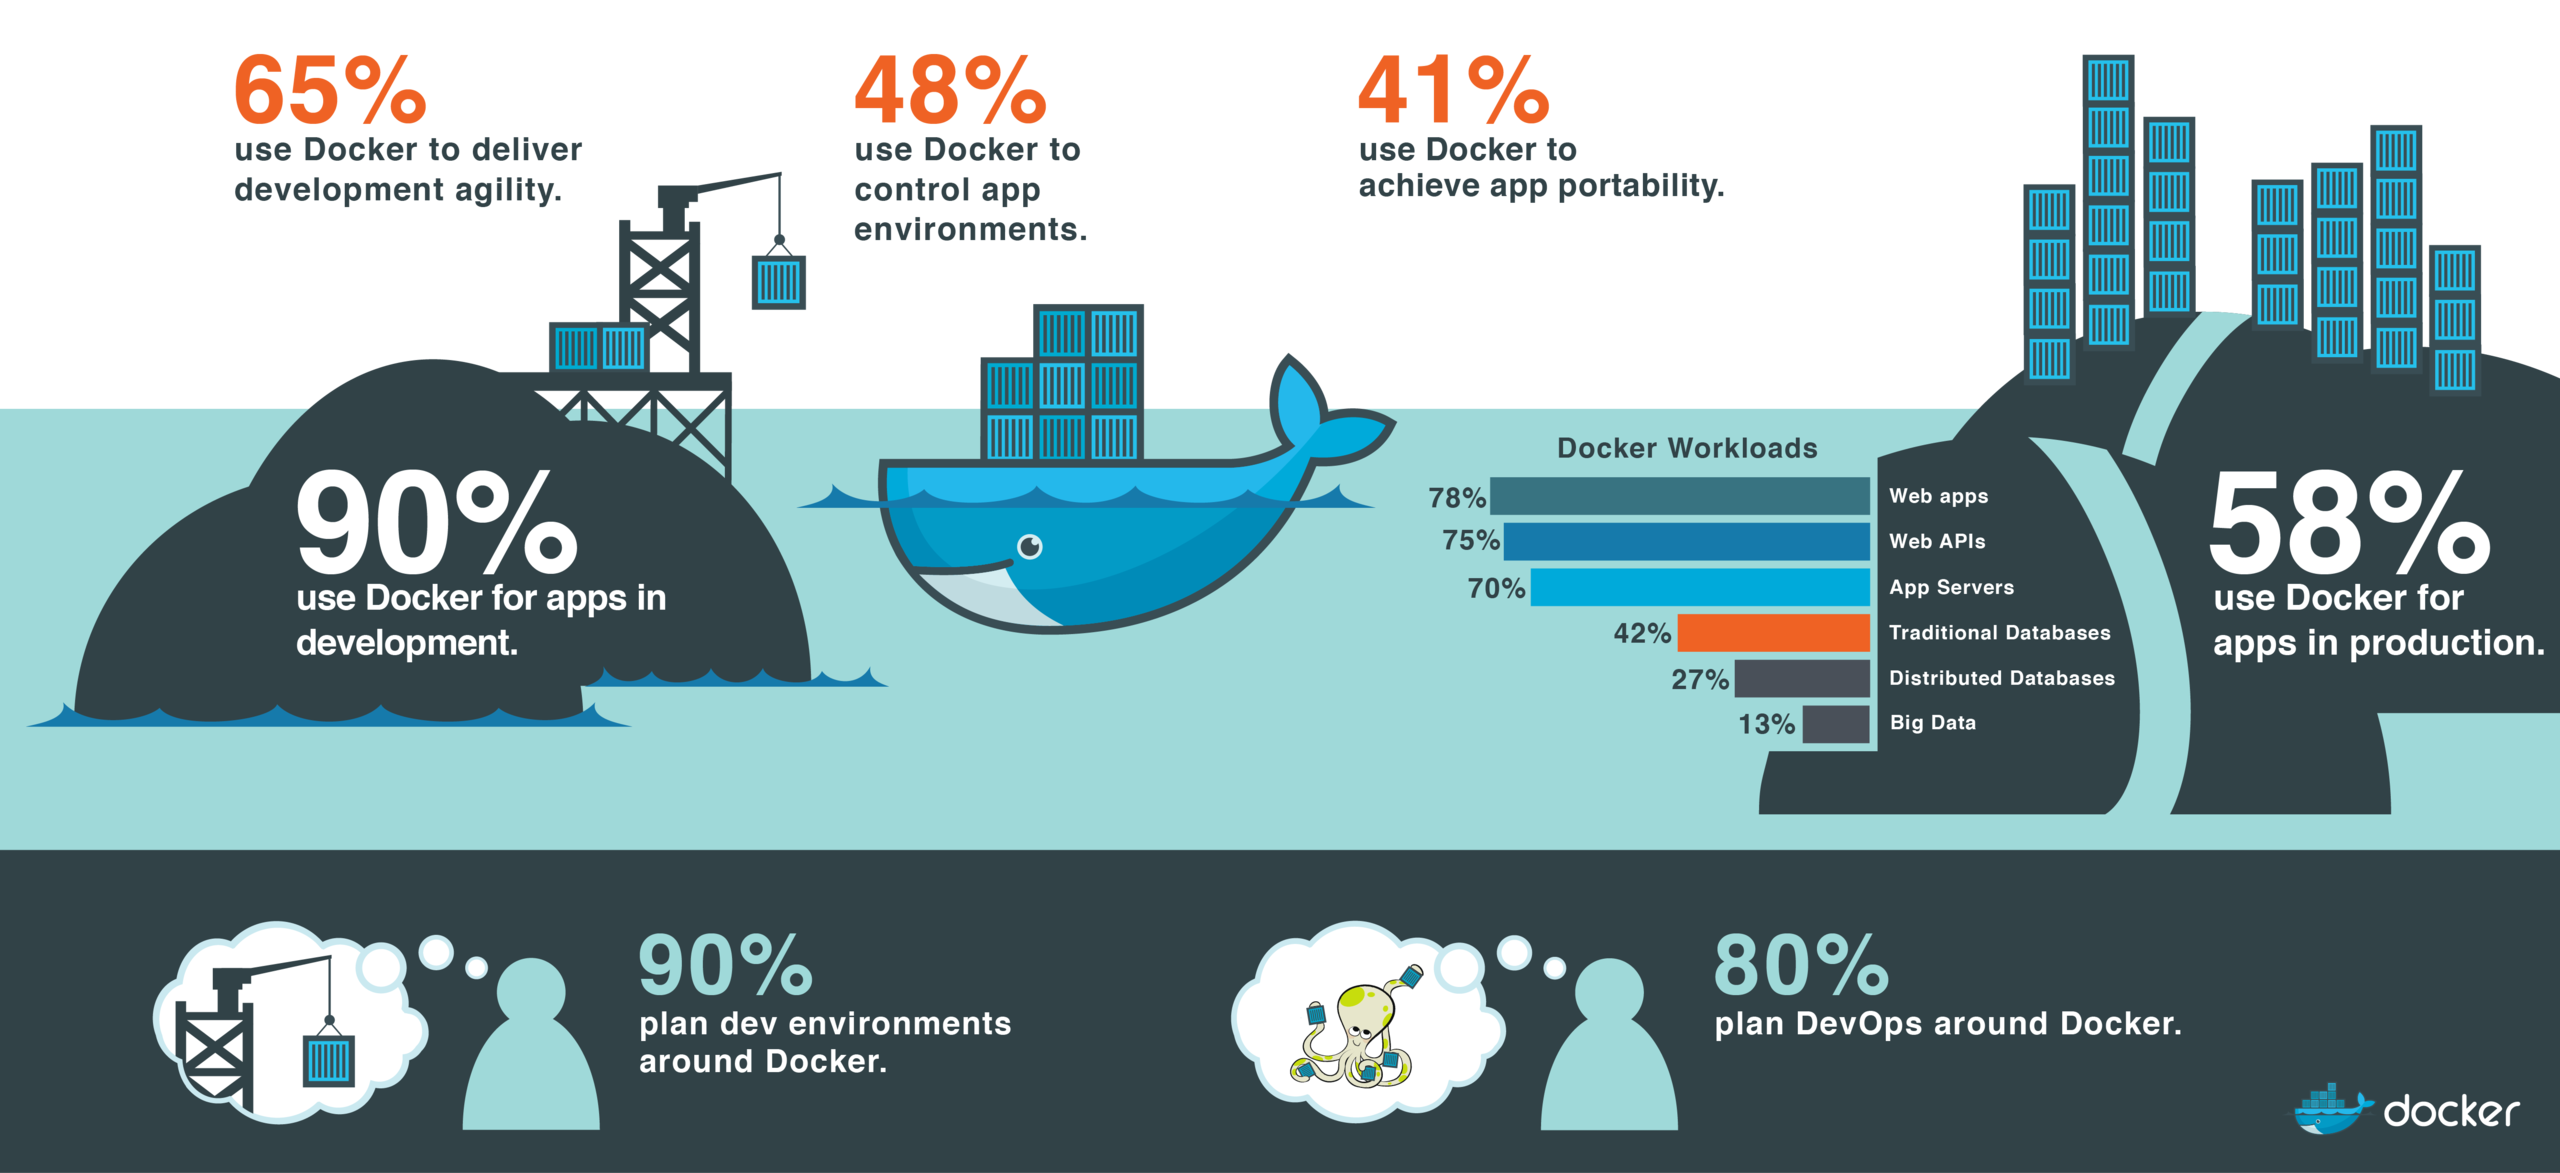
\includegraphics[width=1.0\textwidth]{docker-survey.png}
\caption{Docker Survey Results 2016
}
\end{figure}


\section{Docker Overview}

\URL{https://docs.docker.com/engine/docker-overview/}


\begin{figure}[htb]
\centering
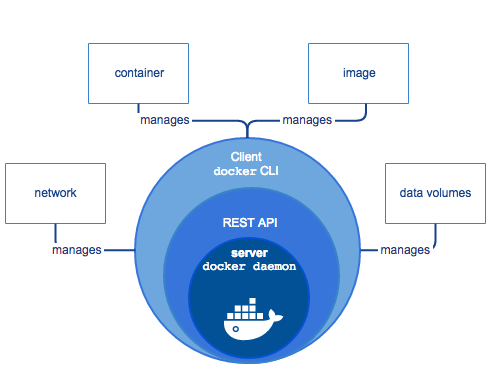
\includegraphics[width=0.5\textwidth]{engine-components-flow.png}
\caption{ Docker Engine Component Flow }
\end{figure}

\begin{figure}[htb]
\centering
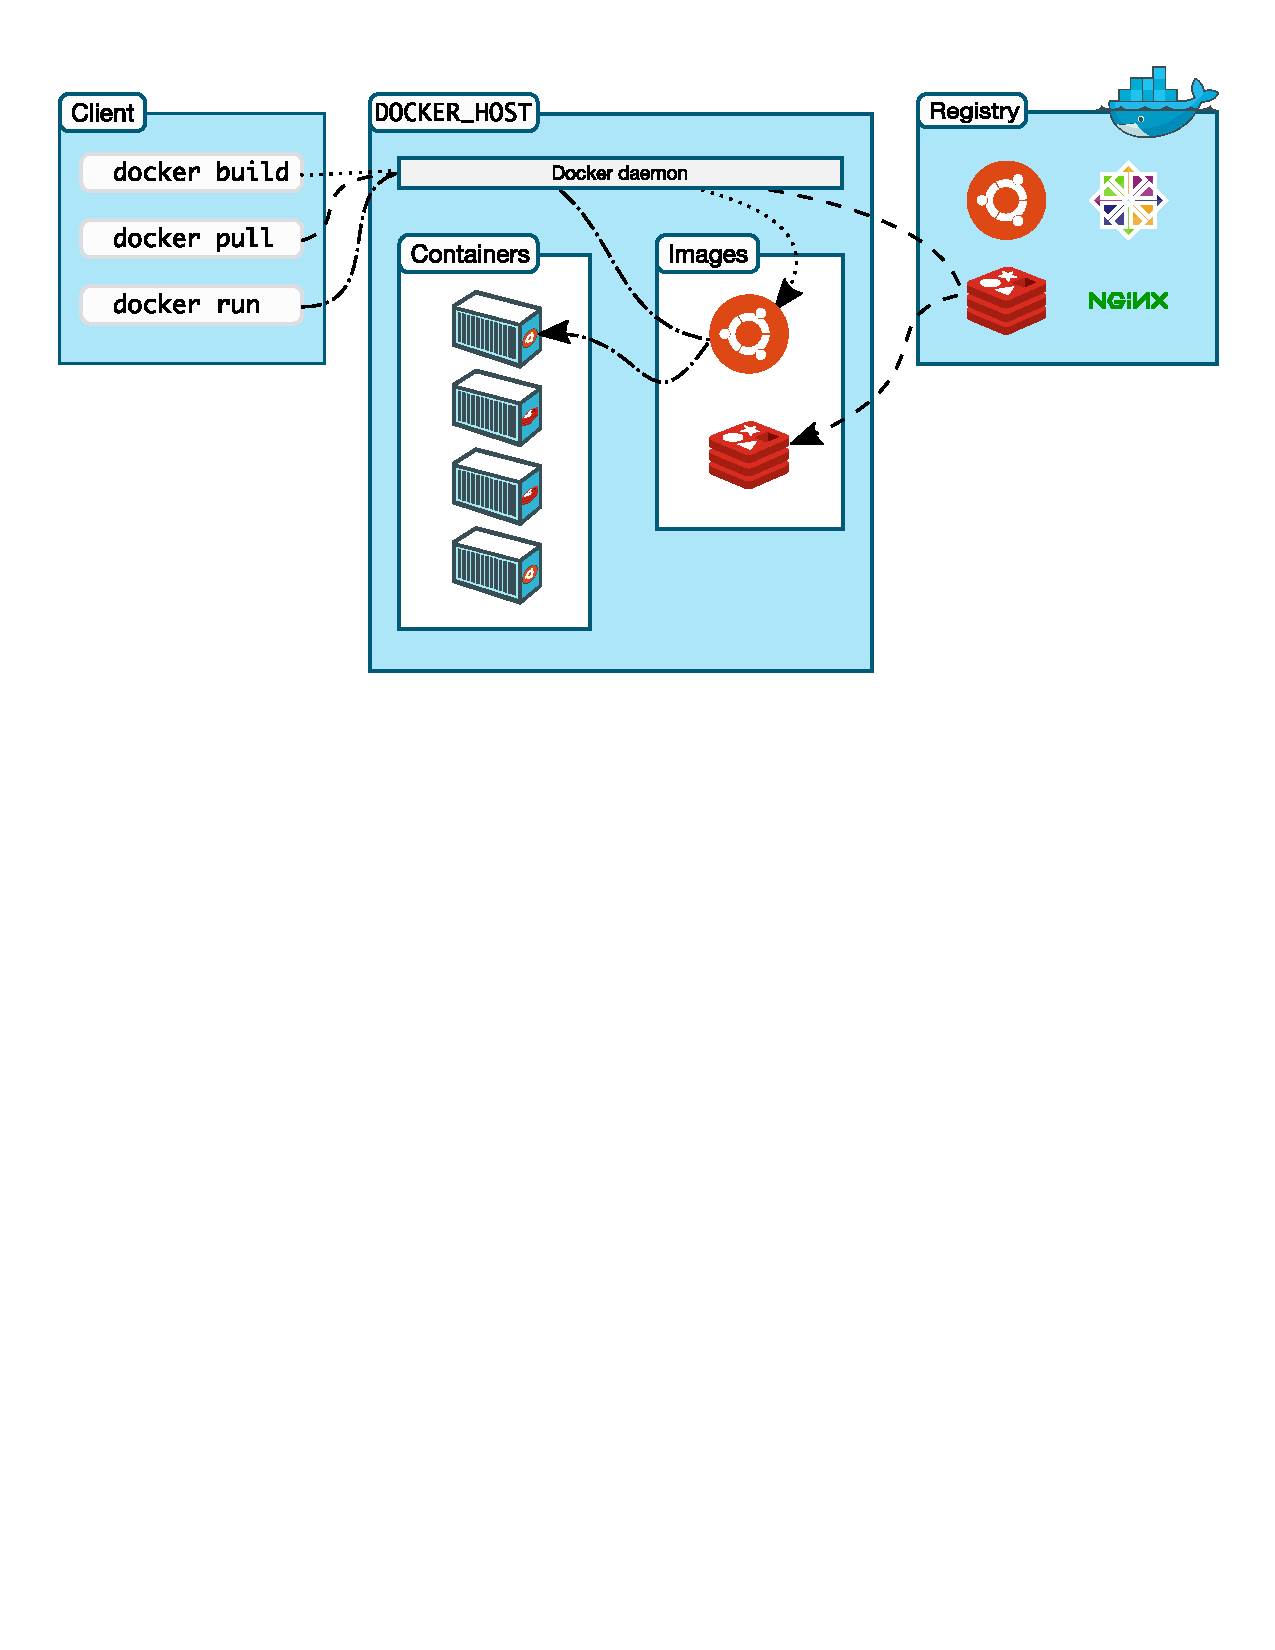
\includegraphics[width=1.0\textwidth]{docker-architecture.pdf}
\caption{ Docker Architecture }
\end{figure}



\section{Container Orchestration Tools: Compare Kubernetes vs Docker Swarm}

\URL{https://platform9.com/blog/compare-kubernetes-vs-docker-swarm/}

\section{Gentle introduction to Containers}

\URL{https://www.slideshare.net/jpetazzo/introduction-docker-linux-containers-lxc}

\section{Tutorialspoint}

\URL{https://www.tutorialspoint.com/docker/index.htm}

\URL{https://www.tutorialspoint.com/docker/docker_tutorial.pdf}

\URL{https://www.tutorialspoint.com/docker/docker_pdf_version.htm}

\section{Tutorial: Docker Swarm on Google Compute Engine}

\URL{https://rominirani.com/docker-swarm-on-google-compute-engine-364765b400ed}

\section{Docker Swarm Tutorial}

https://rominirani.com/docker-swarm-tutorial-b67470cf8872

\section{Spark Cluster}

Scalable Spark Deployment using Kubernetes - Part 8 : Meetup Talk

\URL{http://blog.madhukaraphatak.com/scaling-spark-with-kubernetes-part-1/}
\URL{http://blog.madhukaraphatak.com/scaling-spark-with-kubernetes-part-2/}
\URL{http://blog.madhukaraphatak.com/scaling-spark-with-kubernetes-part-3/}
\URL{http://blog.madhukaraphatak.com/scaling-spark-with-kubernetes-part-4/}
\URL{http://blog.madhukaraphatak.com/scaling-spark-with-kubernetes-part-5/}
\URL{http://blog.madhukaraphatak.com/scaling-spark-with-kubernetes-part-6/}
\URL{http://blog.madhukaraphatak.com/scaling-spark-with-kubernetes-part-7/}
\URL{http://blog.madhukaraphatak.com/scaling-spark-with-kubernetes-part-8/}
\URL{http://blog.madhukaraphatak.com/scaling-spark-with-kubernetes-part-9/}

\chapterimage{pi-cluster.jpg} % Chapter heading image

\chapter{Pi Cluster Form Factor}\label{c:pi-cluster-form-factor}


\section{NAS (1 Pi)}\label{nas-1-pi}

Although a NAS is not really a compute cluster the Pi has used many times to build a
Network Attached Storage (NAS) server. In this configuration a HDD is
attached to the Raspberry and the network features of the Raspberry is
used to access the disk drive via software installed on the PI that
make this easily possible. Many tutorials exists on the Web that help
setting op such a device.

We like to hear from you if you have successfully developed such a NAS
and provide us with such links. Links that may help include:

  \URL{https://hackmypi.com/NASpi.php}


\section{ClusterHat (4 Zero + 1 Pi)}\label{clusterhat-4-zero-1-pi}

The smallest cluster we came across is actually a hybrid cluster in
which 4 Pi zeros attached to a Raspberry Pi 3. Thi sis achieved via an
add on board to the Pi 3 allowing to plug in PI=i Zeros:


  \URL{https://clusterhat.com/}


The Cluster HAT (Hardware Attached on Top) allows to attach 4 Raspberry
Pi Zeros via to be attached to a regular Raspberry PI 3 to simulate a
small cluster.

According to the Web Site it supports the following features:



\begin{itemize}
\item
  USB Gadget Mode: Ethernet and Serial Console.
\item
  Onboard 4 port USB 2.0 hub.
\item
  Raspberry Pi Zeros powered via Controller Pi GPIO (USB optional).
\item
  Individual Raspberry Pi Zero power controlled via * Controller Pi GPIO
  (I2C).
\item
  Connector for Controller Serial Console (FTDI Basic).
\item
  Controller Pi can be rebooted without interrupting power to Pi Zeros
  (network recovers on boot).
\end{itemize}

\begin{figure}
\centering
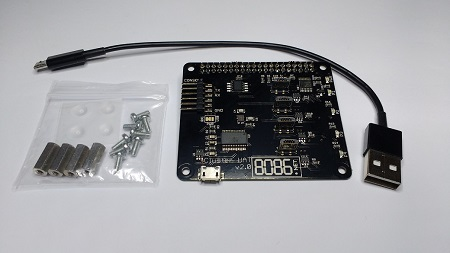
\includegraphics[width=0.5\textwidth]{ClusterHAT-v2-supplied-sm.jpg}
\caption{clusterhat}
\end{figure}



Links:


\URL{https://www.raspberrypi.org/magpi/clusterhat-review-cluster-hat-kit/}{clusterhat
  on raspberrypi.org}


Although this setup seems rather appealing, the issue is with obtaining
Pi Zeros for the regional price of \$5. Typically users can only by one
for that price and must pay shipping. To by more one has to buy a kit
for about \$20. However, for that amount of money it may just be worth
while to get Pi 3's instead of zero's. Nevertheless the formfactor is
rather appealing.

\section{Cluster Case With Cooling (5 Pi)}\label{S:cluster-case-with-cooling-5-pi}

Many instructions on the Web exist describing how to build clusters with
3 or more Pi's. One of the considerations that we have to think about is
that we may run rather demanding applications on such clusters causing
heat issues. To eliminate them we must provide proper cooling. In some
cluster projects cooling is not adequately addressed. Hence we like to
provide an example that discusses in detail how to add a fan and what the
fan has for an impact on the temperature.

\begin{figure}
\centering
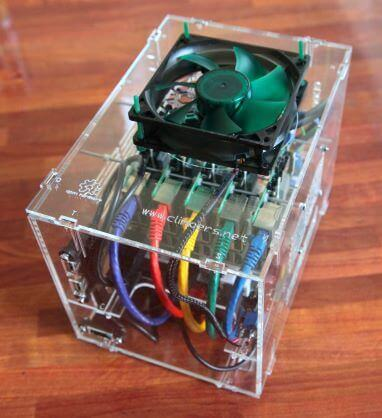
\includegraphics[width=0.5\textwidth]{IMG16_6273_sweb.jpg}
\caption{}
\end{figure}


\URL{http://climbers.net/sbc/add-fan-raspberry-pi/}

\URL{http://climbers.net/sbc/diy-raspberry-pi-3-cluster/}


From the above Web page we find the following information as shown in
Table \ref{F:pi-fan}. From the data in the table it is clear that we
need to keep the Pi from throttling while being in a case by adding a
fan as obvious from experiment No. 2.



\begin{table}[htb]
\caption{Temperature comparision of fan impact}\label{F:pi-fan}
\bigskip
\begin{center}
\begin{tabular}{llllllll}
\hline
No. & Case & Fan & Direction & RPM & Idle & 100\% Load &
Performance\tabularnewline
\hline
1 & no & no & - & - & 41.0C & 75.5C & OK (barely)\tabularnewline
2 & yes & no & - & - & 45.0C & 82.5C & throttles\tabularnewline
3 & yes & 5V & in & unkown & 37.9C & 74.5C & OK (barely)\tabularnewline
4 & yes & 7V & in & 800 & 35.6C & 69.5C & OK\tabularnewline
5 & yes & 12V & in & 1400 & 32.5C & 61.1C & OK\tabularnewline
6 & yes & 7V & out & 800 & 34.5C & 66.4C & OK\tabularnewline
\hline
\end{tabular}
\end{center}
\end{table}




\section{Bitscope Case (40 Pi)}\label{bitscope-case-40-pi}

A company from Australia called BitScope Designs offers a number of
cases that leverage their Pi Blade boards allowing up to four Pis to be
put together and sharing the same power supply. The blades are shown in
Figure b.1. The rack to place 10 of them is shown in Figure b.2.

\begin{figure}
\centering
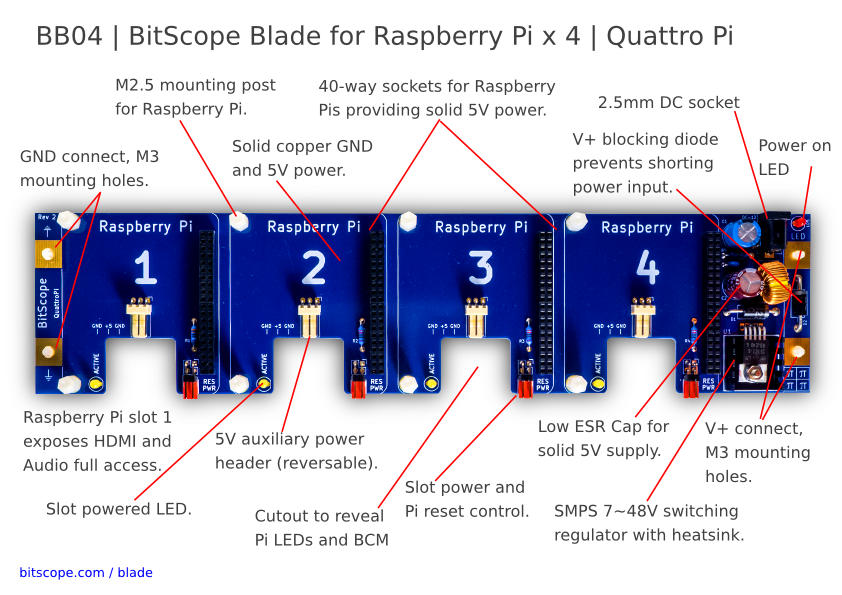
\includegraphics[width=0.3\textwidth]{04.jpg}
\caption{Bitscope blade for 4 Pi's.}
\end{figure}


\begin{figure}
\centering
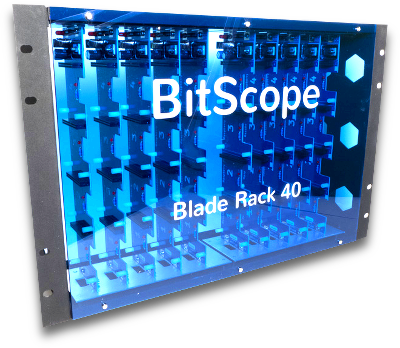
\includegraphics[width=0.3\textwidth]{br40a.png}
\caption{40 Pi Blade rack.}
\end{figure}


The cost of the balde rack is \$ 795.45 + \$60.00 shipping + import tax.
This may originally sound expensive when compared to a single case,
however as we can store 40 Pis in them and they can share the
power-supply and reduce cabeling we think this case is quite interesting
overall due to its price-point of \$20 per Pi.



\section{Bitscope Cluster (144 Pi)}\label{bitscope-cluster-144-pi}

Together with LANL a new cluster module that holds 144 Pis is developed.
This sytem is targeted to be placed into a rack to create a large Pi
cluster. The cost for such a module is about \$15K. Figure
\ref{F:pi-mod-1} shows the
module and Figure \ref{F:pi-mod-2} shows how multiple modules can be placed into a
single rack.

\begin{figure}
\centering
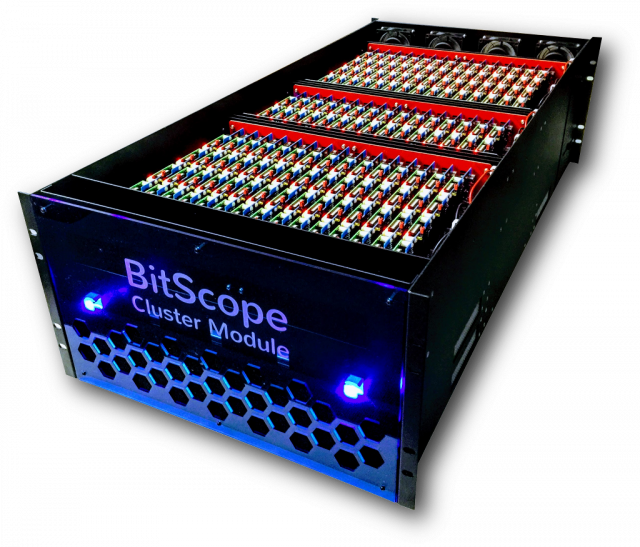
\includegraphics[width=0.5\textwidth]{cluster-module.png}
\caption{Bitscope 144 cluster module.}\label{F:pi-mod-1}
\end{figure}

\begin{figure}
\centering
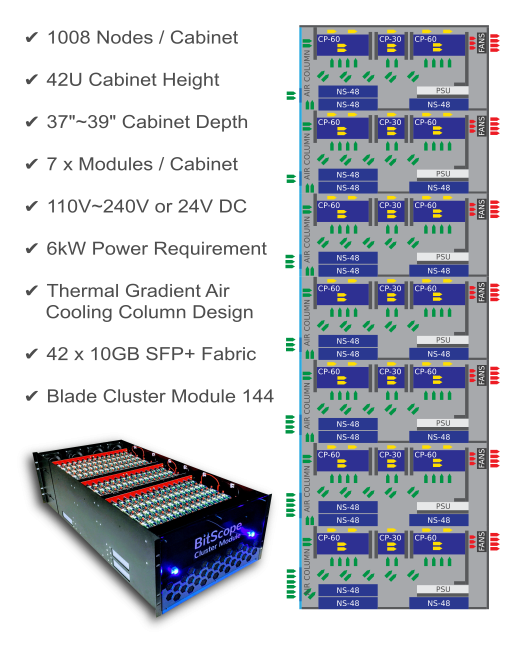
\includegraphics[width=0.5\textwidth]{rack-overview.png}
\caption{Rack placement of multiple Bitscope 144 cluster modules.}\label{F:pi-mod-2}
\end{figure}




\subsection{Links}\label{links}

\URL{https://cluster.bitscope.com/solutions}
\URL{https://www.pcper.com/news/General-Tech/BitScope-Unveils-Raspberry-Pi-Cluster-2880-CPU-Cores-LANL-HPC-RD}
\URL{http://my.bitscope.com/store/}
\URL{http://my.bitscope.com/store/?p=view\&i=item+7}
\URL{http://www.newark.com/bitscope/bb04b/quattro-pi-board-raspberry-pi/dp/95Y0643}
\URL{http://linuxgizmos.com/rpi-expansion-boards-support-up-to-40-pi-clusters/}



\section{Build Your Own 5 Node Pi CLuster}

To experiment with building an elementary cluster one does not need to
have a big budget. Such clusters are often dedicated to research tasks
and are bound into security protocols that do not allow direct
access. Instead it is possible to build such a cluster based on
Raspberry PI's yourself if you are willing to spend the money or if
you have access to PI's that you may loan from your department.

Table \ref{T:picluster-partslist} lists one such possible parts list
that will allow you to build a cluster for up to 5 nodes. However make
sure to buy at least 3 Raspberry PI's with the appropriate memory. At
minimum we recommend you get the 32GB SD card. We do not recommend any
smaller as otherwise you will run out of memory. Additionally, you can
add memory and disks on te USB ports. If you attach a HDD, make sure
it has an external power supply and do not drive it from the USB power
as otherwise the PI becomes unstable.  A fan is at this time not yet
included.

Naturally it is possible to modify the parts list and adapt. If you
find better parts let us know. We have not included any case and you
are welcome to share your suggestions with the class. For a case we
are looking also for a good solution for a fan.

We suggest that when you build the cluster to do it on a table with a
large white paper or board, or a tablecloth and take pictures of the
various stages of the build so we can include it in this document.

Initially we just put rasbian as Operating system on the SD cards and
test out each PI. To do so you will naturally need an SD card writer
that you can hook up to your computer if it does not have one. As you
will have to potentially do this more than once it is not recommended
to buy an SD card with the OS on it. Buy the SD card writer instead so
you can redo the flashing of the card when needed. In addition to the
SD card you need a USB mouse and keyboard and a monitor or TV with
HDMMI port.

Locate setup instructions and write  a tutorial in markdown that we
will include here once it is finished. The tutorial is to be managed
on github.

\TODO{Class: check the network hub if it is a good choice as the one we
  originally chose could not be brought in sufficient quantity.}

\begin{table}[htb]

\caption{Parts list for a Pi cluster, remember you need at least 3
  Raspberry Pis}\label{T:picluster-partslist}
\bigskip


\resizebox{\textwidth}{!}{%
\begin{tabular}{rp{13cm}p{1cm}}
  \hline
  Price   &  Description & URL          \\
  \hline
  \hline
  \$29.99 & 
            Anker 60W 6-Port USB Wall Charger, PowerPort 6 for iPhone 7 / 6s /
            Plus, iPad Pro / Air 2 / mini, Galaxy S7 / S6 / Edge /
            Plus, Note 5 / 4, LG, Nexus, HTC and More  
                         & 
                           \href{https://www.amazon.com/Anker-6-Port-Charger-PowerPort-iPhone/dp/B00P933OJC/ref=pd\_sim\_107\_70?\_encoding=UTF8\&psc=1\&refRID=B1S6V5G0CTJ9NH5G0CRT}{link}
  \\

  \$8.90  & 
            Cat 6 Ethernet Cable 1 ft White ( 6 Pack ) – Flat Internet Network
            Cable – Jadaol Cat 6 Computer Cable short - Cat6 Ethernet
            Patch Lan Cable With &
                                   \href{https://www.amazon.com/Cat-Ethernet-Cable-White-Pack/dp/B01IQWGI0O/ref=sr\_1\_1?s=electronics\&ie=UTF8\&qid=1513699717\&sr=1-1\&keywords=Cat+6+Ethernet+Cable+1+ft+White+\%28+6+Pack+\%29+\%E2\%80\%93+Flat+Internet+Network+Cable+\%E2\%80\%93+Jadaol+Cat+6+Computer+Cable+short+-+Cat6+Ethernet+Patch+Lan+Cable+With\%E2\%80\%A6}{link}  \\

  $^{(1)}$ \$19.99 &  D-link 8-Port Unmanaged Gigabit Switch
            (GO-SW-8G)   & 
                           \href{https://www.amazon.com/D-link-8-Port-Unmanaged-Gigabit-GO-SW-8G/dp/B008PC1MSO}{link}      \\


  \$10.49 &  SanDisk Ultra 32GB microSDHC UHS-I Card with
            Adapter, Grey/Red, Standard Packaging
            (SDSQUNC-032G-GN6MA)
                         & 
                           \href{https://www.amazon.com/SanDisk-microSDHC-Standard-Packaging-SDSQUNC-032G-GN6MA/dp/B010Q57T02/ref=sr\_1\_10?s=pc\&rps=1\&ie=UTF8\&qid=1498443283\&sr=1-10\&refinements=p\_85:2470955011,p\_n\_feature\_two\_browse-bin:6518304011,p\_n\_feature\_keywords\_two\_browse-bin:5947557011}{link}       \\

  \$8.59  & Short USB Cable, OKRAY 10 Pack Colorful Micro
            USB 2.0 Charging Data Sync Cable Cord for
            Samsung, Android Phone and Tablet, Nexus, HTC,
            Nokia, LG, Sony, Many Digital Cameras-0.66ft
            (7.87 Inch) & 
                          \href{https://www.amazon.com/OKRAY-Colorful-Charging-Samsung-Cameras-0-66ft/dp/B00R5GZJR6/ref=sr\_1\_6?s=pc\&ie=UTF8\&qid=1498447476\&sr=1-6\&keywords=micro+usb+cable+1ft}{link}         \\


  \$7.69    & 50 Pcs M2 x 20mm + 5mm Hex Hexagonal Threaded
              Spacer Support
                         & 
                           \href{https://www.amazon.com/20mm-Hexagonal-Threaded-Spacer-Support/dp/B00FH8AB8Q/ref=sr\_1\_9?s=industrial\&ie=UTF8\&qid=1513700337\&sr=1-9\&keywords=hex+spacers+m2+20mm}{link}
  \\

  \$7.99  & Easycargo 15 pcs Raspberry Pi Heatsink Aluminum
            + Copper + 3M 8810 thermal conductive adhesive
            tape for cooling cooler Raspberry Pi 3, Pi 2,
            Pi Model B+
                         & 
                           \href{https://www.amazon.com/Easycargo-Raspberry-Heatsink-Aluminum-conductive/dp/B07217N5LS/ref=sr\_1\_3?s=industrial\&ie=UTF8\&qid=1513700498\&sr=1-3\&keywords=raspberry+pi+3}{link}
  \\

  \$34.49 & Raspberry Pi 3 Model B Motherboard  (you need at least 3 of them)   & 
                                                                                  \href{https://www.amazon.com/Raspberry-Pi-RASPBERRYPI3-MODB-1GB-Model-Motherboard/dp/B01CD5VC92}{link}
  \\

 $^{(2)}$ \$59.99 & 1TB drive   & \href{http://wdlabs.wd.com/products/wd-pidrive-berryboot-edition/}{link}    \\

  \$15.19 & 64GB flash  & \href{https://www.wdc.com/products/wdlabs/wd-pidrive-foundation-edition.html\#WD3750LMCW}{link} \\

  \$6.99  & HDMI Cable, Rankie 2-Pack 6FT Latest Standard
            HDMI 2.0 HDTV Cable - Supports Ethernet, 3D, 4K
            and Audio Return (Black) - R1108
                         & 
                           \href{https://www.amazon.com/Cable-Rankie-2-Pack-Latest-Standard/dp/B00Z07XQ4A/ref=sr\_1\_6?s=wireless\&ie=UTF8\&qid=1513782649\&sr=1-6\&keywords=hdmi+cable+6ft}{link}         \\

  \$12.99  & AUKEY USB C Adapter, USB C to USB 3.0 Adapter
             Aluminum 2 Pack for Samsung Note 8 S8 S8+,
             Google Pixel 2 XL, MacBook Pro, Nexus 6P 5X, LG
             G5 V20 (Gray)
                         & 
                           \href{https://www.amazon.com/Cat-Ethernet-Cable-White-Pack/dp/B01IQWGI0O/ref=pd\_sim\_147\_2?\_encoding=UTF8\&psc=1\&refRID=FZZ7E36666EJPDTH7B6A}{link}     \\

\$19.19 & For Raspberry Pi 3 2 TFT LCD Display, kuman 3.5
   Inch 480x320 TFT Touch Screen Monitor for
   Raspberry Pi Model B B+ A+ A Module SPI
   Interface with Touch Pen SC06
     & 
\href{https://www.amazon.com/Raspberry-Display-kuman-480x320-Interface/dp/B01CNJVG8K/ref=sr\_1\_1?s=electronics\&ie=UTF8\&qid=1513783748\&sr=1-1\&keywords=pi+3+lcd+screen+3.5in}{link} \\
\hline
\end{tabular}
}
\smallskip

{\footnotesize (1) items were replaced with similar item}\\
{\footnotesize (2) item was not avialable}

\end{table}



\subsection{Exercise}\label{E:cluster-pi}

In case you do not have access to multiple PIs conduct the Single Pi experiment.

\section{Single Pi}


You have been presented in Section
\ref{S:cluster-case-with-cooling-5-pi} with a table that compares
tempreatures. Your task is to identify issues with the experiment and
the table.  Furthermore we like you to rerun a temperature experiment
in the entire class.

\TODO{Gregor: Add IoT section and PI configuration}

\begin{enumerate}
\item
  Get a PI3 modeL B, an HDMI cable, a power supply, a case. Such a
  configuration is listed in the IoT section. 
\item
  Buy or manufacture a case of your choice. You can use a 3d-printer
  if you have one available.
\item
  Conduct a temperature experiment.
\end{enumerate}

Exercises:


\begin{exercise}
\label{E:Exercise.Pi.Single.1} What temperature measurement is missing from the
  table. 
\end{exercise}

\begin{exercise}
\label{E:.Pi.Single.2} How would you create an experiment under {\em load}.
\end{exercise}

\begin{exercise}
\label{E:.Pi.Single.3} How would you create an experiment to which all
  students in different classes could contribute their values? Can the
  cloud be used?
\end{exercise}

\begin{exercise}
\label{E:.Pi.Single.4} Collect the information from all class members
  using cloud services.
\end{exercise}

\begin{exercise}
\label{E:.Pi.Single.5} Identify who to use the VPN server so you
  can use your Laptop instead of a TV or computer monitor. Write a tutorial.
\end{exercise}


Discussion of this assignment is to be executed openly in
class. Points will be issued only once the class agrees upon an
experiment.

This exercise is not only to learn about the behaviour of the Pi, but
also about how to coordinate experiments with a large number of
students.

\section{Small Cluster Single Pi}

In this set of exercises we will be building a small Raspberry Pi
cluster. All of you will have to do Exercise.Pi.Cluster.Build, as well
as one of the tasks related to Swarm, kubernetes or Spark.

It is important that you write down all steps very carefully as you
are expected to use the steps to develop an automated deployment. For
your cluster. Your tutorial will be tested by other groups and easy of
installation completness, and correctness will be evaluated.  Teams
that find issues and improve deployment tutorials will receive points.
TA's will also replicate these steps to identify a fair evaluation
without bias.


\begin{exercise}

\label{E:.Pi.Cluster.Build} Build groups of up to 5 people. Make a
  plan on what needs to be done to build the cluster and develop a
  schedule. Include in this plan (a) obtaining the material the
  hardware build, (b) the installation of the operating system (c) the
  testing of the system (d) familiarizing with the OS.
\end{exercise}

\begin{exercise}

\label{E:.Pi.Cluster.DockerSwarm} Install a docker Swarm cluster on your
  PI. Develop a tutorial in markdown and mind plagiarism. Contribute your tutorial
  to this document to get acknowledged and credit. Work with others in
  class to coordinate a single tutorial.
\end{exercise}

\begin{exercise}

\label{E:.Pi.Cluster.Kubernetes} Install a kubernetes cluster on your
  PI. Develop a tutorial in markdown and mind plagiarism. Contribute your tutorial
  to this document to get acknowledged and credit. Work with others in
  class to coordinate a single tutorial.
  
\label{E:.Pi.Cluster.Spark} Install a spark cluster on your
  PI. Develop a tutorial in markdown and mind plagiarism. Contribute your tutorial
  to this document to get acknowledged and credit. Work with others in
  class to coordinate a single tutorial.
\end{exercise}




%

\chapter{Sentient Architecture}

\FILENAME\

\begin{figure}
\centering
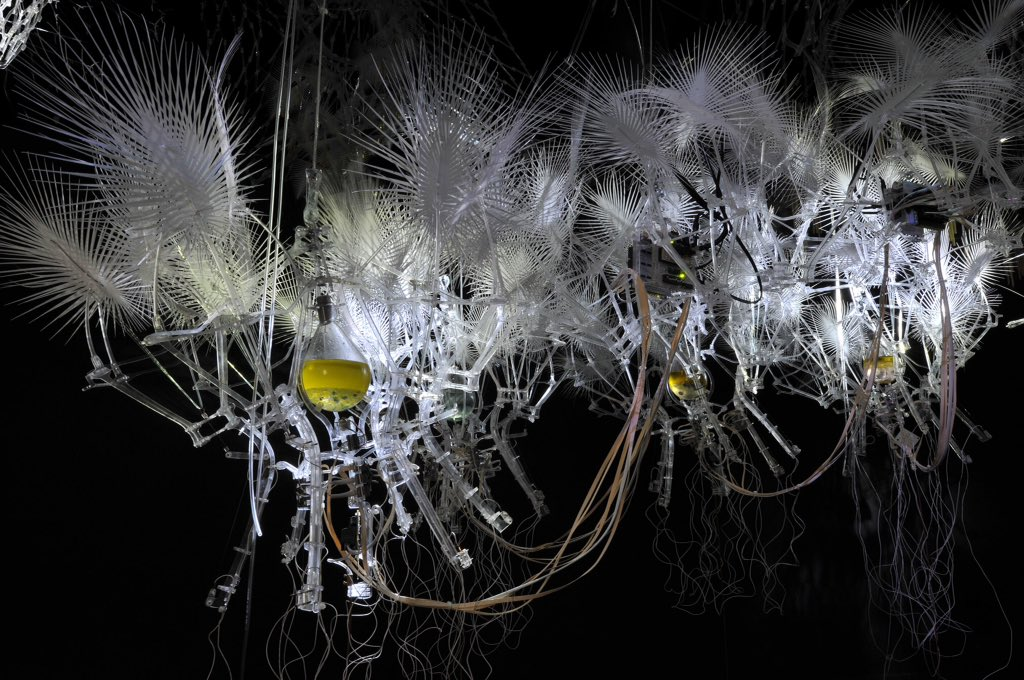
\includegraphics[width=\columnwidth]{images/sentient.jpeg}
\caption{Sentinent Architecture: Source: \url{https://nicolatriscott.files.wordpress.com/2016/03/caaqt-euyam-jpm.jpg}} 
\end{figure}

\section{Introduction}

What is it

\section{Existing Deployments}

list	existing deployments

\section{Impact}

why is it important

not only science, 

\section{Integration into Cloud Computing and Big Data}

how dos it for to cloud computing and big data (Gregor can do that)


\section{Development}
S Architecture in practice


\subsection{Snowwhite and the Seven$^{+1}$ Dwarfs}

The ISE department at Indiana University has obtained eight dendrites
that were assambled by a number of students so they can be used in
class and in research projects. These dendrites can be accessed in
Smith Research Center and allow students and faculty members to
experiment with them. They are bare dendrites and have no
electronics on them. Hence, you will need a hardware device to
interact with.

The reason we named them \textit{Snowwhite and the Seven$^{+1}$ Dwarfs}
is based on the fact that the dendrites are white, and they need to be
interact with  somone. Beacuse of the white color we name the controll
unit snowwhite. The dendrites that are interacting with it are called
dwarfs as this just fits to the name snowwhite. As we actually have 8
and not 7 we added $^{+1}$.


We do not recommend to directly attach the
wires to boards, as they will draw too much power and destroy the
boards. Instead you will need a relay that you controll that itself
controlls the dendrite These can be:

\begin{description}

\item[Arduino:] These boards very simple but provide relative good
  protection of the output links. The disadvantage is that its
  interface is in C.

\item[Teensy] Whatever is now on it TBD

\item[Raspberry Pi] We recommend to use a Raspberry Pi as it has a
  great operating system and is more suited for additional analysis of
  data within an Edge Computing network than the other two choices. It
  also allows you to use python which is clearly a pluss as most of
  the material presented here are in Python.

\end{description}


\begin{figure}
\centering
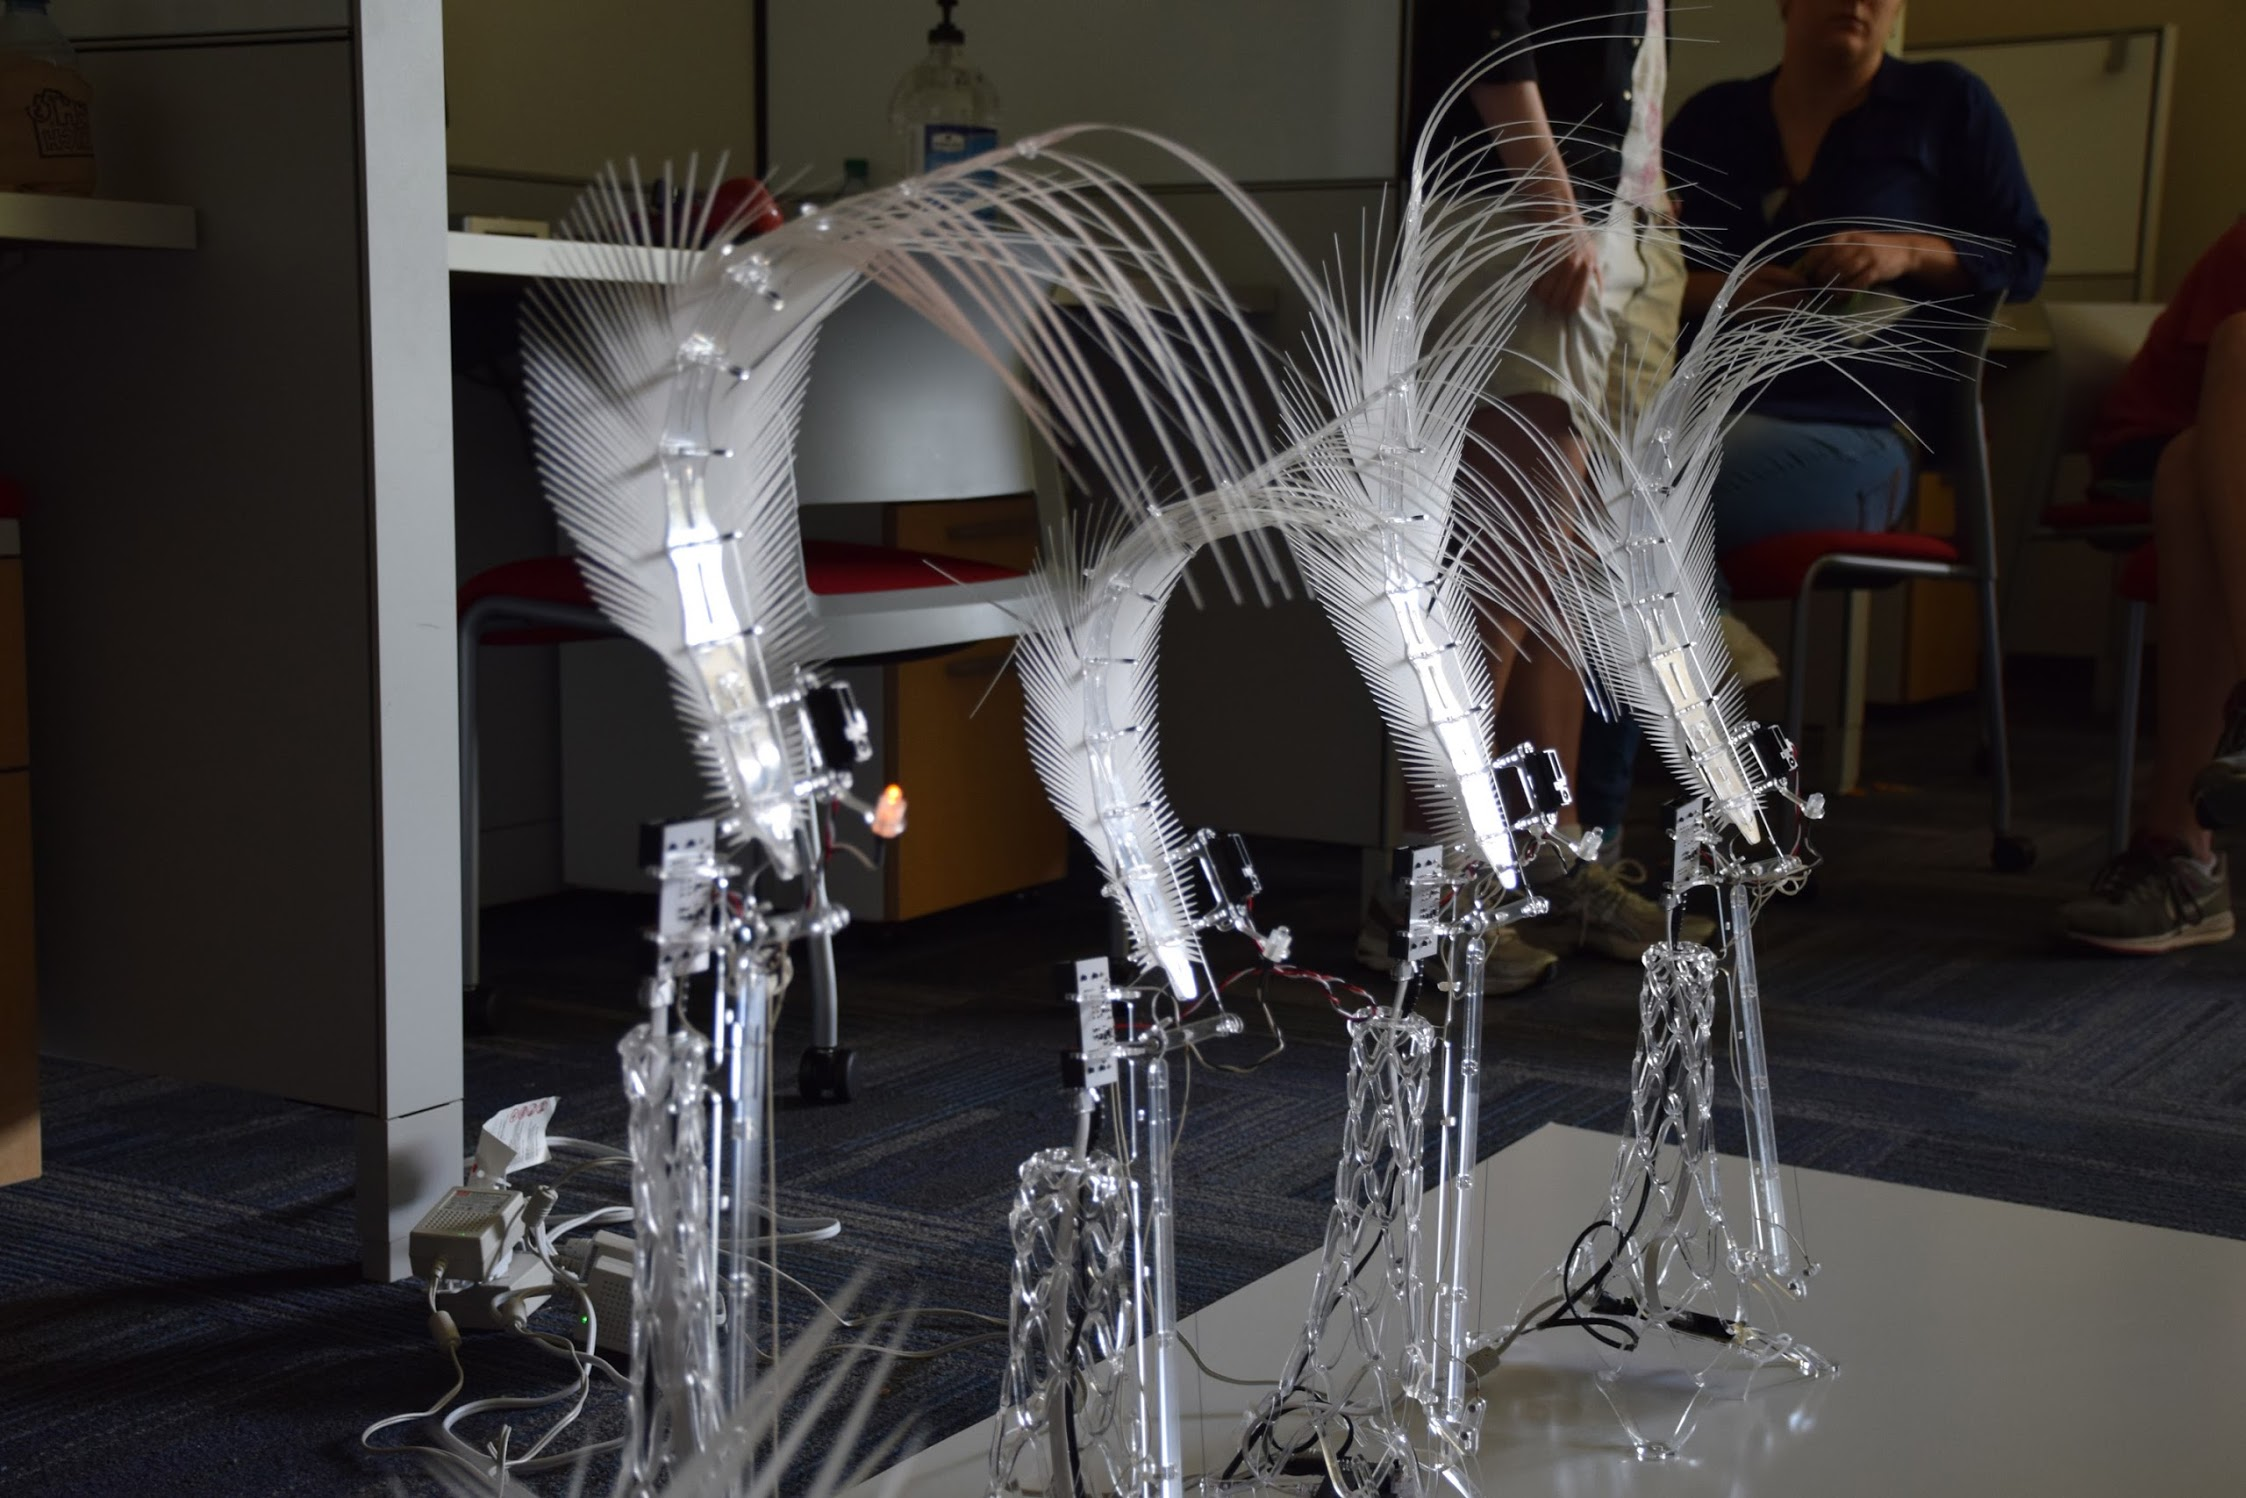
\includegraphics[width=\columnwidth]{images/snowwhite.jpg}
\caption{Snowwhite and the Seven$^{+1}$  Dwarfs}
\label{F:snowwhite}
\end{figure}


\subsection{Liddy Hall Installation}

architecture drawing


\section{Sentinent Cloudmesh}

	Gregor provides introduction to cloudmesh (probably just pointer to other section)

	Gregor provides introduction to cloudmesh.pi 

	Introduction to parallel programming in python (TBD)

	Towards the Cloudmesh Parallel S development environment


\paragraph{Snowwhite and the Seven$^{+1}$ Dwarfs}

Test environment (8 dendrites)

\paragraph{Liddy Hall}

Andreas dsecribes how we program them 

(Andreas provides)


than we use cloudmesh to interface with them, maybe we need to just
show how we integrate them into mqtt (this is snowhwite) and than we  
can progrem them from another pi

	Test environment Liddy hall 

\section{Alternative Boards}

\subsection{Mega 2560}

``The MEGA 2560 is designed for more complex projects. With 54 digital
I/O pins, 16 analog inputs and a larger space for your sketch it is
the recommended board for 3D printers and robotics projects. This
gives your projects plenty of room and opportunities.'' 
\url{https://store.arduino.cc/usa/arduino-mega-2560-rev3}
A nice case such as the one offered at Amazon will provide good
protection \url{https://www.amazon.com/Eleduino-Arduino-Mega-2560-Enclosure/dp/B016QE46RQ}


\begin{figure}
\centering
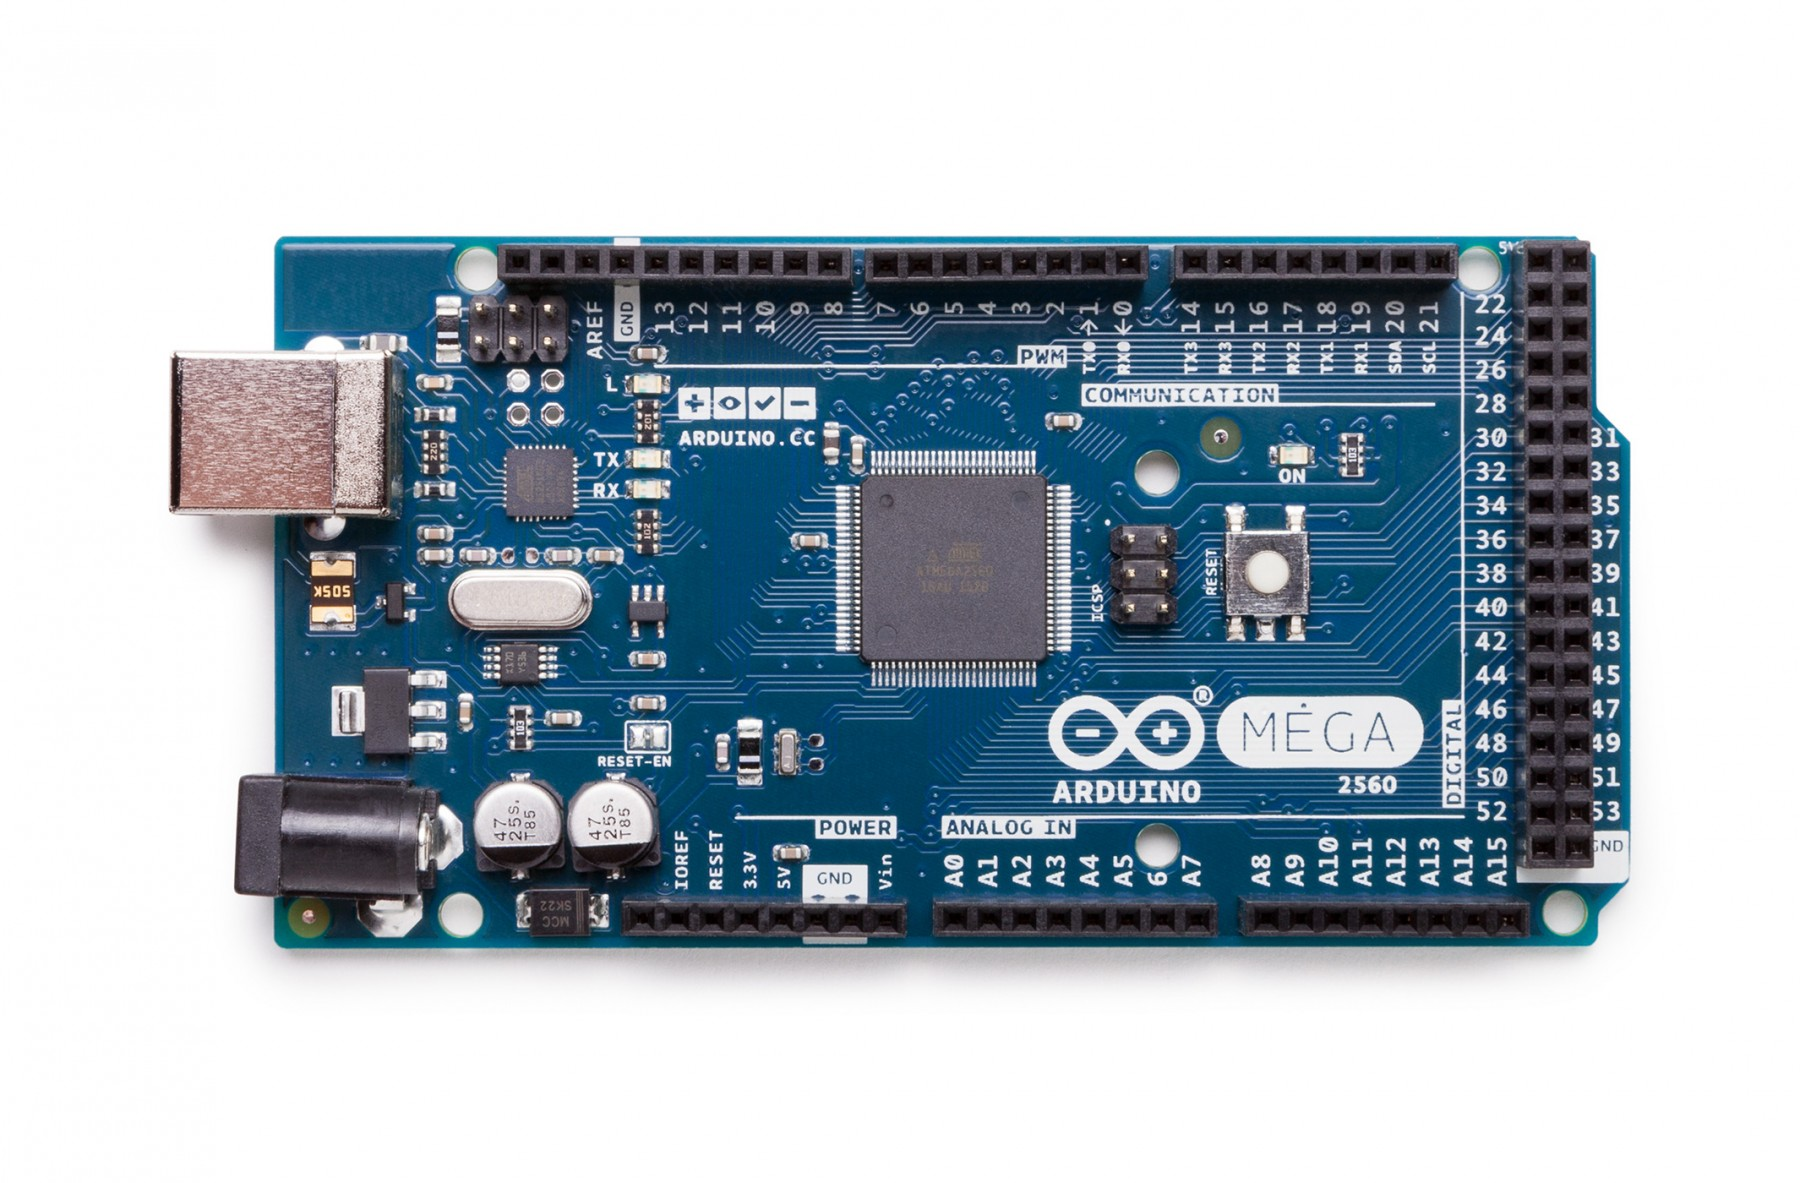
\includegraphics[width=0.25\columnwidth]{images/mega2560.jpg}
\caption{MEGA 2560}
\label{F:mega2560}
\end{figure}


\subsection{Programming with Teensy}

``The Teensy is a complete USB-based microcontroller development
system, in a very small footprint, capable of implementing many types
of projects. All programming is done via the USB port.'' Source: \url{https://www.pjrc.com/teensy/}

Current state of programming (whateverthey have)

Which version



\section{Exercises}

\begin{description}

\item[Sentinent.1] Build dendrite. In this excersise you will be
  building a dendrite that you can add to the available pool of dendrites.
\item[Sentinent.2.1] Develop cloudmesh sensor/actuary. In this excersise
  you will be developing an actuator ar sensor interface in object
  oriented programming methodology. You can see many examples in
  cloudmesh.py on github,com. You will pick a sensor you have access
  to and that is not already included in cloudmesh.pi. 
\item[Sentinent.2.2] If you do
  prefer using another board, the option may exist do develp an
  interface for the sensor or actuator for this device. If OO
  programming is not available for that board, a clean design based on
  functions must be provided. However we believe this is mor complex
  than using the Pi. 
\item[Sentinent.3.1] Develop an mqtt based event publisher and
  subscription service. Use first LEDs to test your service before you
  hook up relays and dendrites.
\item[Sentinent.3.2] Hook up the dendrites to mqtt and controll them
\item[Sentinent.4] Develop sensors that interact with the dendrites
\item[Sentient.5] Explore the Page at
  \url{https://www.intorobotics.com/alternative-arduino-boards/} that
  lists a number of PI/Arduino alteranative boards provide a non
  plagiarized table for this chapter and evaluate which could be
  viable alternatives. If you have one of them we like you to provide
  a documentation on how to integrate them with the dendrites.

\end{description}

 



%----------------------------------------------------------------------------------------

\cite{www-sharelatex}

%%%%%%%%%%%%%%%%%%%%%%%%%%%%%%%%%%%%%%%%%%%%%%%%%%%%%%%%%%%%%%%%%%%%%%
\chapterimage{water.png} 
\chapter*{Bibliography}
%%%%%%%%%%%%%%%%%%%%%%%%%%%%%%%%%%%%%%%%%%%%%%%%%%%%%%%%%%%%%%%%%%%%%%
\addcontentsline{toc}{chapter}{\textcolor{ocre}{Bibliography}}

%------------------------------------------------

%\section*{Articles}
%\addcontentsline{toc}{section}{Articles}
%\printbibliography[heading=bibempty,type=article]

%------------------------------------------------

%\section*{Books}
%\addcontentsline{toc}{section}{Books}
%\printbibliography[heading=bibempty,type=book]

\section*{References}
\printbibliography[heading=bibempty]


%%%%%%%%%%%%%%%%%%%%%%%%%%%%%%%%%%%%%%%%%%%%%%%%%%%%%%%%%%%%%%%%%%%%%%
%	INDEX
%%%%%%%%%%%%%%%%%%%%%%%%%%%%%%%%%%%%%%%%%%%%%%%%%%%%%%%%%%%%%%%%%%%%%%

\cleardoublepage
\phantomsection
\setlength{\columnsep}{0.75cm}
\addcontentsline{toc}{chapter}{\textcolor{ocre}{Index}}
\printindex


\end{document}
